\pagebreak

\thispagestyle{empty}

\movetoevenpage
\thispagestyle{empty}
\begin{absolutelynopagebreak}
\begin{vplace}
\begin{figure}[H]
\begin{adjustwidth}{-1.40cm}{}
  \centering
  \vspace*{-2.4cm}
  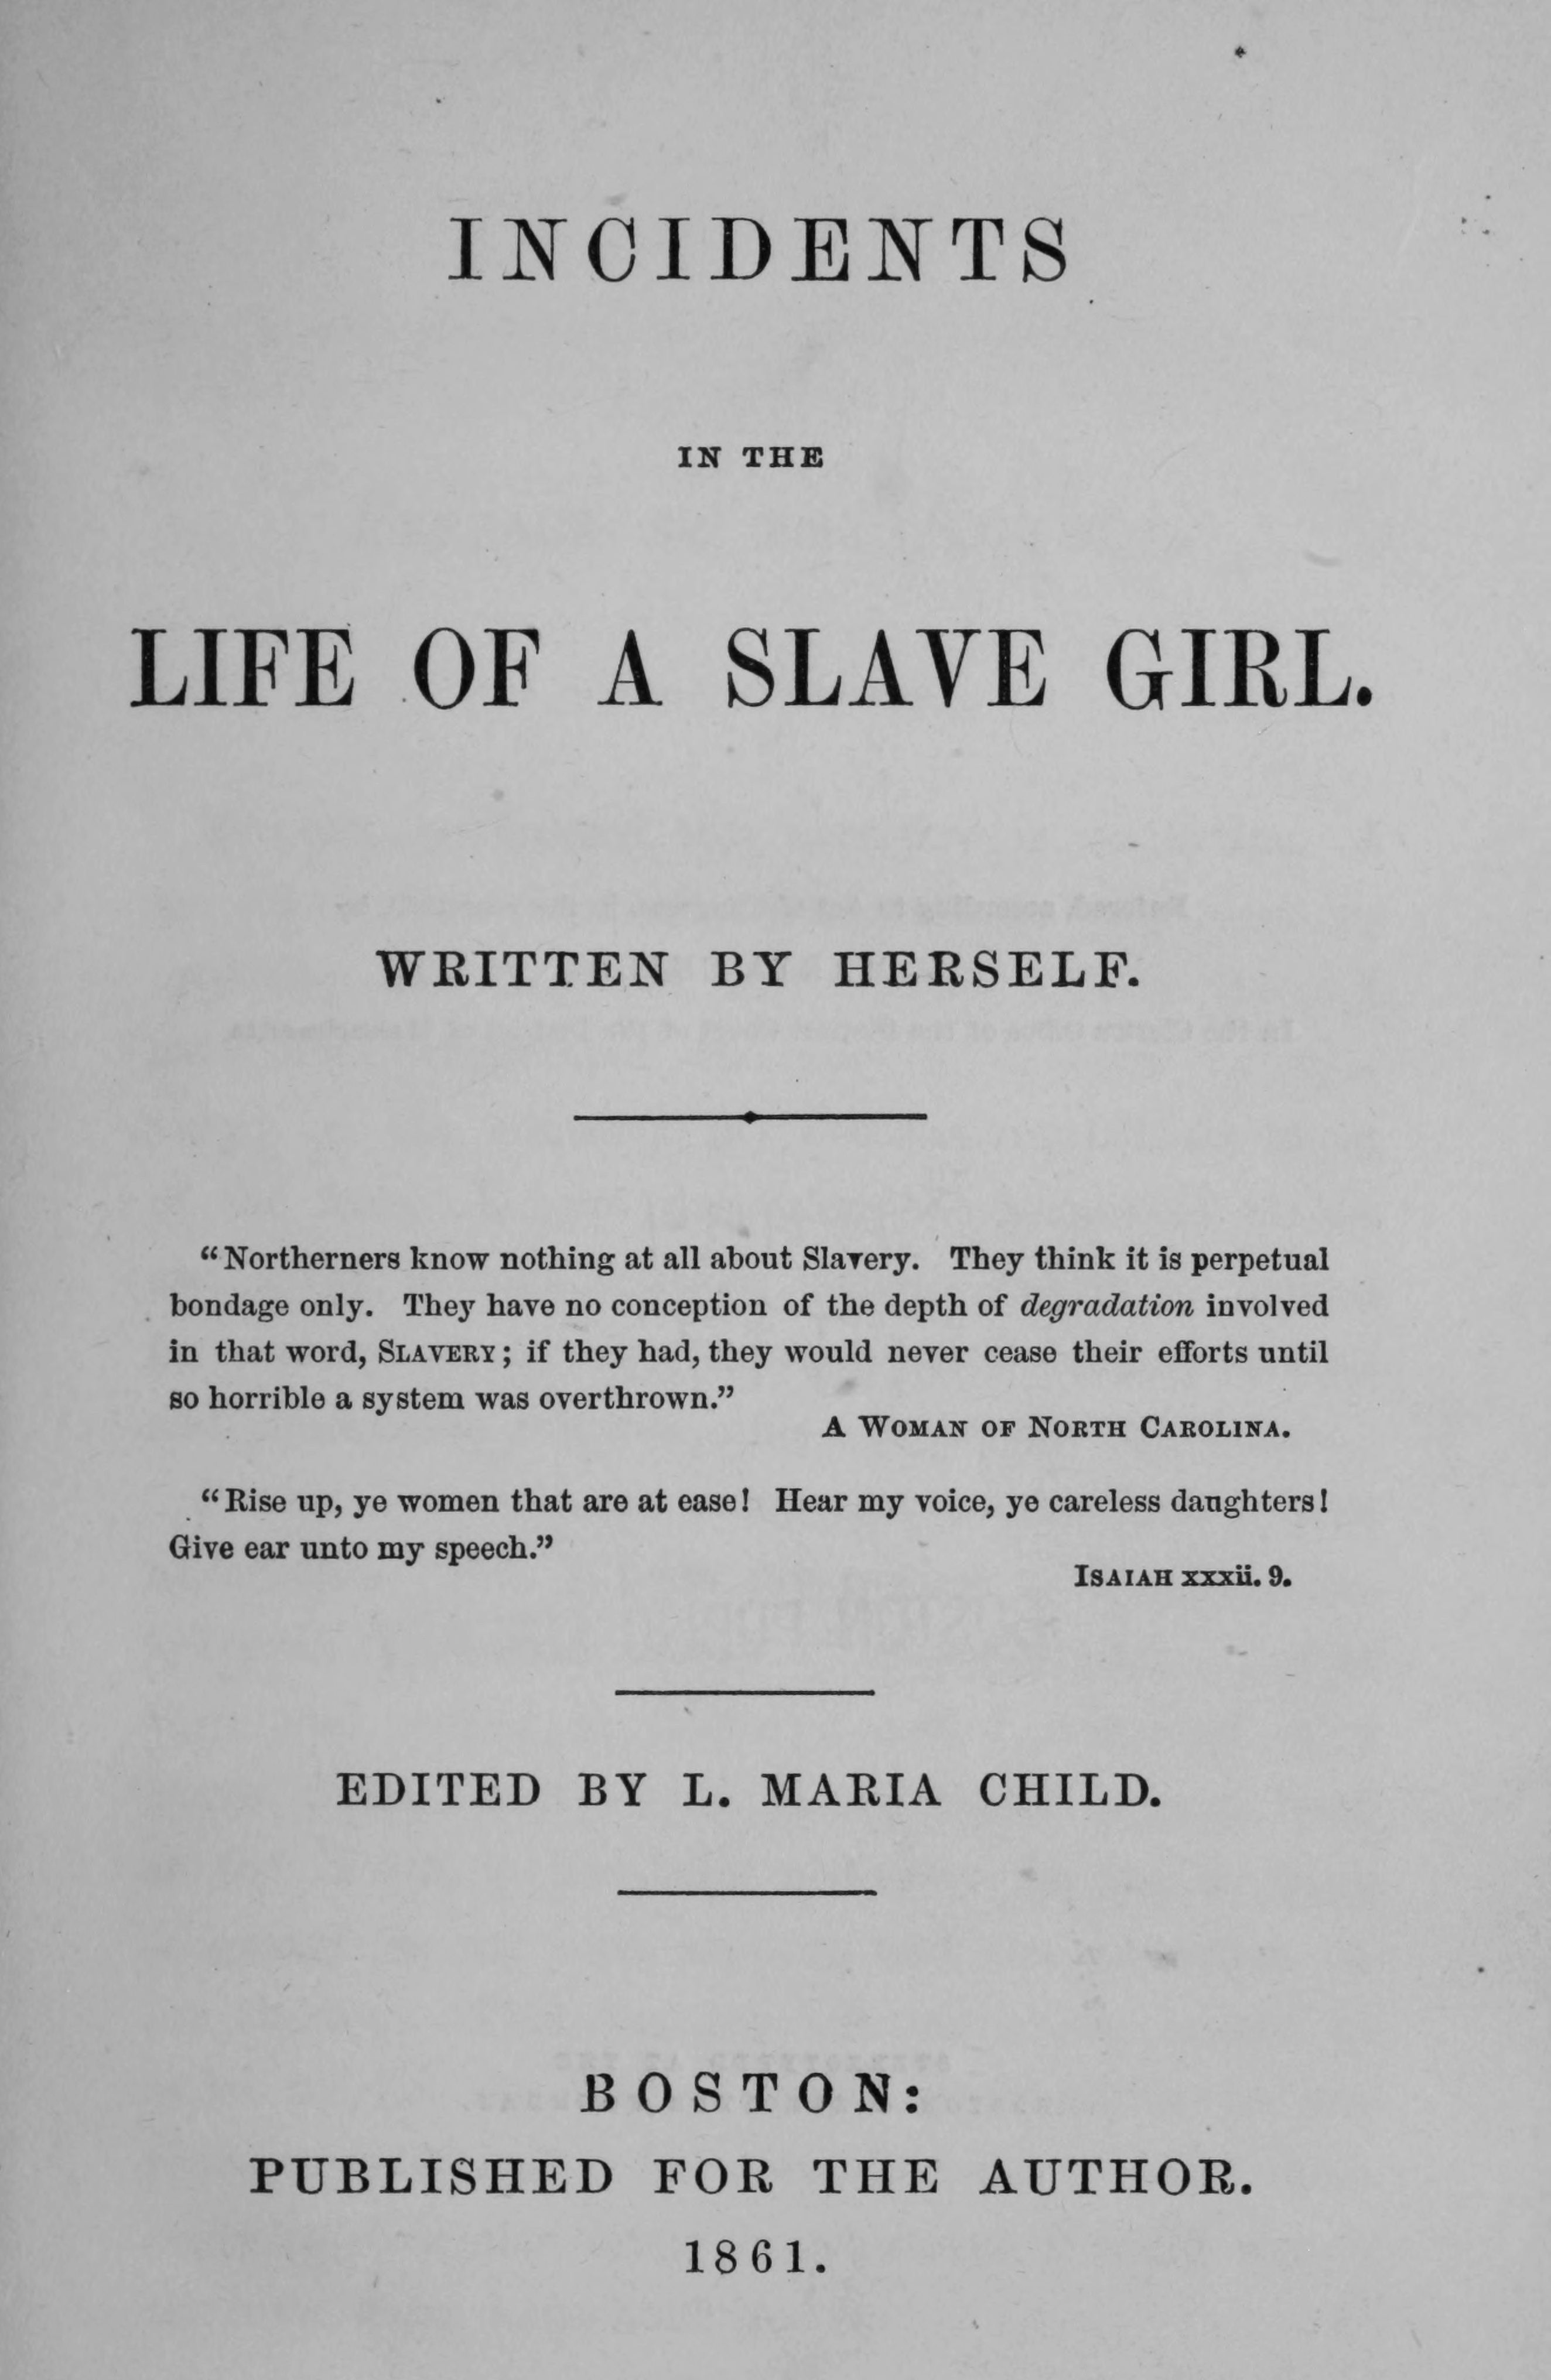
\includegraphics[width=125mm]{./imgs/front.jpg}  
  %\hfill
\end{adjustwidth}
  \caption{Frontispício da primeira edição da autobiografia de Harriet Jacobs, publicada em Boston em 1861.}
\end{figure}
\end{vplace}

\thispagestyle{empty}
\end{absolutelynopagebreak}

\addcontentsline{toc}{part}{Incidentes da vida de uma escrava}
\part*{Incidentes da vida de uma escrava, escritos por ela mesma}

\chapter*{}

\thispagestyle{empty}
\vspace*{\fill}

\epigraph{\emph{Os nortistas não sabem nada sobre a
Escravidão. Eles imaginam que é apenas uma servidão perpétua. Eles não
fazem ideia da degradação abismal que envolve essa palavra,
escravidão. Se tivessem, nunca cessariam seus esforços até a derrocada
de um sistema tão horrível.}}{\textsc{uma mulher da carolina do norte}}

\epigraph{\emph{Levantai"-vos, mulheres, que estais
sossegadas, e ouvi a minha voz; e vós, filhas, que estais tão seguras,
inclinai os ouvidos às minhas palavras.}}{\textsc{isaías 32:9}}

\chapter*{Prefácio da autora}
\addcontentsline{toc}{chapter}{Prefácio da autora}
\hedramarkboth{Prefácio da autora}{}

A leitora pode ficar segura de que esta
narrativa não é ficcional. Estou ciente de que algumas de minhas
aventuras podem parecer incríveis; ainda assim, elas são estritamente
verdadeiras. Não exagerei os males infligidos pela Escravidão; pelo
contrário, minhas descrições não estão à altura dos fatos. Ocultei os
nomes dos lugares e dei às personagens nomes fictícios. Não tenho por
que fazer segredo em benefício próprio, mas considerei que esse modo de
agir seria uma bondade e uma consideração para com outros.

Gostaria de ser mais competente na
tarefa que assumi, mas confio que minhas leitoras escusarão minhas
deficiências à luz das circunstâncias. Nasci e fui criada na Escravidão
e morei em um Estado Escravista por vinte e sete anos. Desde que cheguei
ao norte, me foi necessário trabalhar arduamente para o meu próprio
sustento e para a educação dos meus filhos. Isso não me deixou tempo
livre para compensar a perda das primeiras oportunidades de educação, e
também me forçou a escrever estas páginas em intervalos irregulares,
sempre que conseguia achar uma hora entre os deveres domésticos.

Quando cheguei à Filadélfia, o Bispo
Paine me aconselhou a publicar um breve relato da minha vida, mas minha
resposta foi que eu não teria a competência necessária para esse
empreendimento. Embora minha mente tenha se aperfeiçoado desde então, minha
opinião continua a mesma; ainda assim, confio que meus motivos
compensarão o que poderia parecer presunção de minha parte. Não escrevi
minhas experiências para chamar a atenção para mim mesma; pelo
contrário, teria sido mais agradável continuar em silêncio sobre minha
própria história. Também não pretendo fazer com que a leitora simpatize
comigo por causa do que sofri. Desejo apenas e ardentemente fazer com
que as mulheres do norte entendam a condição de dois milhões de mulheres
do sul que ainda estão em ferros, sofrendo o que sofri, e a maioria
delas muito mais. Quero agregar meu testemunho às penas mais capazes e
ajudar a convencer o povo dos Estados Livres do que é a Escravidão de
fato. É apenas por experiência que se entende as profundezas, o negrume,
a podridão desse poço de abominações. Que a bênção de Deus caia sobre
esse esforço imperfeito em nome do meu povo perseguido!

\chapter*{Introdução à primeira edição}
\addcontentsline{toc}{chapter}{Introdução à primeira edição
\medskip}
\hedramarkboth{Introdução à primeira edição}{L. Maria Child}

\begin{flushright}
\versal{L. MARIA CHILD}
\end{flushright}

Conheço pessoalmente a autora da
autobiografia a seguir e sua conversa e seus modos me inspiram
confiança. Ela passou boa parte
dos últimos dezessete anos morando com uma família distinta de Nova York
e se comportou de tal forma a conquistar o mais alto grau da sua estima.
Esse fato é o bastante, sem mais credenciais sobre a sua índole. Creio
que aqueles que a conhecem não ficarão predispostos a duvidar da sua
veracidade, apesar de alguns incidentes da sua história serem mais
românticos do que os de uma obra de ficção.

Revisei o manuscrito a seu pedido, mas
minhas alterações foram realizadas principalmente para fins de
condensação e organização. Não adicionei nada aos incidentes nem alterei
o significado de suas observações extremamente pertinentes. Com raras
exceções, tanto as ideias quanto o linguajar são dela. Podei alguns
excessos, mas além disso não tive nenhum motivo para alterar o modo
vívido e dramático como ela conta a própria história. Os nomes das
pessoas e dos lugares me são conhecidos, mas os oculto com bons motivos.

Naturalmente, provocará surpresa que
uma mulher criada no seio da Escravidão saiba escrever tão bem, mas as
circunstâncias explicam o fato. Em primeiro lugar, a natureza a dotou de
grande perspicácia. Segundo, a senhora com a qual ela morou até os doze
anos de idade era uma pessoa bondosa, tendo ensinado a autora a ler e a
escrever. Terceiro, ela encontrou circunstâncias favoráveis após chegar
ao norte, travando contato frequente com pessoas inteligentes que se
interessavam pelo seu bem"-estar e estavam dispostas a lhe oferecer
oportunidades para o autoaperfeiçoamento.

Sei muito bem que muitos me acusarão de
falta de decoro por apresentar estas páginas ao público, pois as
experiências dessa mulher inteligente e sofredora pertencem a uma
categoria que alguns chamariam de assuntos delicados, e outros de
indelicados. Essa fase peculiar da Escravidão normalmente se mantém
oculta, mas o público merece conhecer esses traços monstruosos, então
assumo a responsabilidade de desvelá"-la. Faço isso pelo bem das minhas
irmãs cativas, que sofrem males tão terríveis que nossas orelhas são
delicadas demais para escutar. Assim ajo na esperança de inspirar nas
mulheres conscientes e escrupulosas do norte o senso do seu dever no
exercício da influência moral na questão da Escravidão em todas as
ocasiões possíveis. Tomo essa decisão na esperança de que todos os
homens que lerem esta narrativa jurarão solenemente perante a Deus que,
na medida que tiverem o poder de impedi"-lo,
nenhum fugitivo da Escravidão \enlargethispage{\textheight}
jamais será enviado de volta para padecer naquele antro abominável de
corrupção e crueldade.


\chapter*{Infância}
\addcontentsline{toc}{chapter}{Infância}
\hedramarkboth{ Infância}{}

Nasci escrava, mas nunca soube disso
até passarem seis anos de uma infância feliz. Meu pai era um
carpinteiro, considerado tão inteligente e habilidoso nessa profissão
que, quando edifícios fora do comum precisavam ser construídos, ele era
chamado de pontos distantes para ser o líder dos trabalhadores. Sob a
condição de pagar à sua senhora duzentos dólares ao ano e sustentar a si
mesmo, ela permitia que ele exercesse sua profissão e administrasse sua
própria vida. Seu grande desejo era comprar os filhos, mas apesar de ter
diversas oferecido seu dinheiro suado para tanto, ele nunca teve
sucesso. A tez dos meus pais era um tom claro de amarelo"-acastanhado e
os dois eram chamados de mulatos. Eles moravam juntos em um lar
confortável e, apesar de sermos todos escravos, eu era tão
carinhosamente protegida que jamais sonhava ser uma peça de mercadoria,
confiada a eles para proteção, sujeita a ser pedida de volta a qualquer
momento. Eu tinha um irmão dois anos mais novo, William, uma criança
inteligente e afetuosa. Meu outro grande tesouro era minha avó materna,
uma mulher incrível em diversos aspectos. Ela era filha de um fazendeiro
da Carolina do Sul que, ao morrer, libertara a mãe dela e os três
filhos, dando"-lhes dinheiro suficiente para ir a St.\,Augustine, onde
tinham parentes. Isso ocorreu durante a Guerra Revolucionária; eles
foram capturados no caminho, levados de volta e vendidos a compradores
diferentes. Essa era a história que minha avó costumava contar, mas não
lembro de todos os detalhes. Ela era muito menina quando foi capturada e
vendida para o gerente de um grande hotel. Muito ouvi ela contar sobre
as dificuldades que sofreu na infância. Contudo, à medida que foi
crescendo, ela demonstrou tamanha inteligência e tamanha fidelidade que
seu senhor e senhora foram forçados a perceber que seria do seu
interesse tomar muito cuidado de uma propriedade tão valiosa quanto ela.
Minha avó se tornou indispensável na residência, atuando em todas as
funções, de cozinheira e costureira até a ama de leite. Ela recebia
muitos elogios pelos pratos que preparava, e seus biscoitos ficaram tão
famosos na vizinhança que muita gente os cobiçava. Em consequência dessa
busca constante, ela pediu à sua senhora permissão para assar biscoitos
à noite, depois que todo o serviço da casa estivesse pronto; e ela
obteve a permissão, desde que usasse o lucro para vestir a si mesma e
aos filhos. Sob essas condições, após trabalhar duro o dia inteiro para
a senhora, ela começou a preparar suas fornadas da meia"-noite, auxiliada
pelos dois filhos mais velhos. O negócio foi rentável; a cada ano ela
poupava um pouco, sempre economizando em um fundo para a compra dos
filhos. Quando seu senhor morreu, a propriedade foi dividida entre seus
herdeiros. O dote da viúva era o hotel, que ela continuou a administrar.
Minha avó continuou a ser escrava a seu serviço, mas seus filhos foram
divididos entre os filhos do senhor. Como ela tinha cinco, Benjamin, o
mais jovem, foi vendido para que cada um dos herdeiros recebesse uma
porção igual de cada dólar e cada centavo. A diferença entre as nossas
idades era tão pouca que ele mais parecia meu irmão do que meu tio.
Benjamin era um rapaz bonito e inteligente, e quase branco, pois herdara
a tez que derivava dos ancestrais anglo"-saxões de minha avó. Apesar de
ter apenas dez anos, ele obteve o preço de 720 dólares. Sua venda foi um
golpe terrível para a minha avó, mas ela era uma mulher naturalmente
cheia de esperança e passou a trabalhar com energia redobrada, confiando
que um dia seria capaz de comprar alguns dos filhos. Ela havia guardado
300 dólares, que sua senhora um dia pediu de empréstimo, prometendo
devolver em breve. O leitor provavelmente sabe que nenhuma promessa ou
palavra escrita dada um escravo é vinculante. De acordo com as leis
sulistas, o escravo, por \emph{ser} propriedade, não pode \emph{ter}
propriedades. Quando minha avó emprestou seu dinheiro suado à senhora,
ela estava confiando unicamente na honra desta. A honra de um escravista
perante uma escrava!

A essa avó devo inúmeros confortos. Meu
irmão Willie e eu sempre recebíamos porções dos biscoitos, bolos e
compotas que ela fazia para vender. Quando deixamos de ser crianças,
passamos a dever a ela por serviços muito mais importantes.

Essas foram as circunstâncias
anormalmente fortuitas da minha primeira infância. Quando tinha seis
anos, minha mãe morreu; foi então que descobri, pelas conversas ao meu
redor, que era escrava. A senhora
da minha mãe era a filha da senhora da minha avó. Ela era irmã de
criação da minha mãe; ambas foram alimentadas no seio da minha avó. Na
verdade, minha mãe fora desmamada aos três meses de idade para que a
filha da senhora pudesse se alimentar o suficiente. Elas brincavam
juntas quando crianças e, depois de adultas, minha mãe se tornou a
criada fiel da irmã de criação mais branca. No leito de morte, ela ouviu
da senhora a promessa de que seus filhos nunca passariam necessidade;
enquanto viveu, ela cumpriu sua palavra. Todos falavam com afeto da
minha falecida mãe, que fora escrava apenas em nome, mas que tinha
natureza nobre e feminina. Eu chorei por ela, e minha mente infantil se
preocupava com a ideia de quem passaria a cuidar de mim e do meu
irmãozinho. Fui informada que moraria com a senhora, e o que encontrei
foi um lar feliz. Nenhum dever trabalhoso ou desagradável me era
imposto. Minha senhora era tão bondosa comigo que sempre ficava contente
em atender seus pedidos e orgulhosa em trabalhar por ela tanto quanto
minha juventude permitia. Eu passava horas sentada ao seu lado,
costurando incansavelmente, com meu coração tão livre de preocupações
quanto qualquer criança branca que nascera livre. Quando ela achava que
eu estava cansada, me mandava sair para correr e pular; e assim eu ia,
para colher flores ou frutinhas para decorar a sala.
Foram dias felizes, felizes demais
para durar. A criança escrava não pensava no amanhã, mas logo surgiu a
desgraça que sempre aguarda todo o ser humano nascido para ser
propriedade alheia.

Quando eu tinha quase doze anos de
idade, minha boa senhora adoeceu e morreu. Enquanto assistia seu rosto
empalidecer e seus olhos nublarem, como eu rezava no fundo do coração
para que ela sobrevivesse! Eu a amava, pois ela fora quase uma mãe para
mim. Minhas orações não foram atendidas. Ela morreu e foi enterrada no
adro da igreja, onde todos os dias minhas lágrimas caíam sobre o seu
túmulo.

Fui mandada para a casa da minha avó
para passar uma semana. Agora eu já tinha idade o suficiente para
começar a pensar no futuro, e me perguntava constantemente o que fariam
comigo. Tinha certeza de que nunca encontraria outra senhora tão bondosa
quanto a que morrera. Ela prometera à minha mãe no leito de morte que
nada nunca faltaria aos filhos; quando me lembrava disso, e das muitas
demonstrações do afeto que ela tinha por mim, era inevitável nutrir a
esperança de que ela teria me libertado. Meus amigos tinham quase
certeza de que seria assim. Eles achavam que ela deveria ter me
libertado, considerando o amor e o serviço fiel de minha mãe. Mas, ah!
Todos sabemos que a memória de uma escrava fiel nada vale para salvar
seus filhos do leiloeiro.

Após um breve período de suspense, o
testamento da minha senhora foi aberto e então descobrimos que ela havia
me deixado para a filha da irmã, uma menina de cinco anos. Assim
desapareceram nossas esperanças. Minha senhora me ensinara os preceitos
da Palavra de Deus: ``Amarás o teu próximo como a ti mesmo''. ``Assim,
em tudo, façam aos outros o que vocês querem que eles lhes façam''. Mas
eu era sua escrava, imagino que ela não reconhecia em mim um próximo. Eu
daria tudo para apagar da minha memória essa grande ofensa. Quando
criança, eu amava minha senhora; e agora, rememorando os dias felizes
que passei com ela, tento pensar com menos amargura sobre esse ato de
injustiça. Enquanto estava com ela, ela me ensinou a ler e a escrever; e
por esse privilégio, tão raramente concedido a um escravo, eu abençoo
sua memória.

Ela
possuía poucos escravos e, ao morrer, estes foram todos distribuídos
entre seus parentes. Cinco deles eram filhos da minha avó e haviam
compartilhado do mesmo leite que nutrira os filhos da sua mãe. Apesar
dos longos anos de serviço fiel prestado pela minha avó para seus
proprietários, nenhum dos seus filhos escapou do leilão. Nenhuma dessas
máquinas que respiram o sopro de Deus vale mais, aos olhos de seus
senhores, do que o algodão no campo ou os cavalos no estábulo.

\chapter*{O novo senhor e a nova senhora}
\addcontentsline{toc}{chapter}{O novo senhor e a nova senhora}
\hedramarkboth{ O novo senhor e a nova senhora}{}

O Dr.\,Flint, um médico da vizinhança,
havia casado com a irmã da minha senhora, e agora eu era propriedade da
sua filhinha. Não foi sem queixumes que me preparei para meu novo lar; e
o que aumentava minha infelicidade era o fato de que meu irmão William
fora comprado pela mesma família. Meu pai, pela sua natureza e também
pelo hábito de realizar negócios como um mecânico de grande habilidade,
tinha mais sentimentos de homem livre do que era comum entre os
escravos. Meu irmão era um menino orgulhoso e, sendo criado sob tais
influências, odiava continuamente o nome de senhor e de senhora. Um dia,
quando seu pai e sua senhora o chamaram ao mesmo tempo, ele hesitou
entre os dois, confuso sobre qual dos dois tinha o direito maior à sua
obediência. Ele finalmente concluiu que deveria ir para a sua senhora.
Quando meu pai o repreendeu por isso, ele respondeu:

--- Vocês dois me chamaram e eu não sabia quem eu devia procurar
primeiro.

--- Você é \emph{meu} filho --- nosso
pai respondeu. --- Quando eu chamo, você deve vir imediatamente, mesmo
que tenha que cruzar fogo e água.

Pobre Willie! Ele estava prestes a
aprender sua primeira lição de obediência a um senhor. Nossa avó tentou
nos animar com palavras otimistas, e estas encontraram eco nos corações
crédulos da juventude.

Quando entramos em nosso novo lar,
fomos recebidos por olhares frios, palavras frias e modos frios. Ficamos
felizes quando a noite chegou. Deitada em minha cama estreita, eu chorei
e gemi, me sentindo sozinha e desconsolada.

Eu estava lá havia quase um ano quando
uma amiga muito querida foi enterrada. Enquanto a terra caía sobre o
caixão da única filha, ouvi sua mãe soluçar e comecei a me afastar da
cova, sentindo gratidão para ainda ter quem amar. Foi quando encontrei
minha avó.

--- Vem comigo, Linda.

Pelo tom de voz, eu sabia que algo triste acontecera. Ela me afastou do
resto das pessoas e anunciou:

--- Minha filha, seu pai está morto.

Morto! Era inacreditável. Ele morrera tão de repente, eu nem sabia que
ele estava doente. Fui para a casa com a minha avó. Meu coração se
rebelou contra Deus, que havia me tirado mãe, pai, senhora e amiga. A
boa avó tentou me confortar.

--- Quem sabe os planos de Deus? Talvez tenha sido bondade poupá"-los do
tempo ruim que está por vir.

Anos depois, ainda penso muito nisso. Ela prometera ser mãe para os
netos, enquanto lhe fosse permitido; fortalecida pelo seu amor, voltei
para a casa do meu senhor. Achei que teria permissão de ir até a casa do
meu pai na manhã seguinte, mas recebi a ordem de buscar flores para
decorar a casa da minha senhora para uma festa naquela noite. Passei o
dia colhendo e engrinaldando flores enquanto o cadáver do meu pai
descansava a menos de uma milha de distância. E meus donos lá se
importavam com isso? Ele era uma reles propriedade. Além do mais, eles
achavam que ele havia mimado os filhos, ensinando"-os a achar que eram
seres humanos. Era uma doutrina blasfema para um escravo ensinar,
presunçosa da parte dele e perigosa para os senhores de escravos.

No dia seguinte, acompanhei seus restos
até a cova humilde ao lado daquela onde repousava minha mãe querida.
Havia quem conhecesse o valor de meu pai e respeitasse sua memória.

Agora meu novo lar parecia mais
melancólico do que nunca. As risadas dos escravinhos eram ríspidas e
cruéis. Era egoísmo meu sentir isso da alegria alheia. Meu irmão andava
com uma cara fechada e séria.

--- Coragem, Willie --- tentei confortá"-lo. --- Dias melhores virão.

--- Você não sabe de nada, Linda ---
ele respondeu. --- Vamos ter que ficar aqui pelo resto da vida. Nunca
vamos ser livres.

Argumentei
que estávamos ficando mais velhos e mais fortes, e que talvez não
demorasse para que pudéssemos alugar nosso próprio tempo. Desse jeito,
ganharíamos dinheiro para comprar nossa liberdade. William declarou que
falar era muito mais fácil do que fazer; além do mais, ele não tinha a
intenção de \emph{comprar} a sua liberdade. O assunto era tema de
controvérsia diária entre nós.

As refeições dos escravos recebiam
pouca atenção na casa do Dr.\,Flint. Se eles conseguiam arranjar alguma
comida enquanto havia, muito bem. Eu não me incomodava em nada nesse
quesito, pois em minhas diversas tarefas eu costumava passar pela casa
da minha avó, onde sempre havia algo de sobra para mim. Frequentemente,
ameaçavam me punir quando parava lá; e minha vó, para evitar que eu me
demorasse, ficava me esperando junto ao portão com algo para me servir
de desjejum ou jantar. É a \emph{ela} que devo todos os meus confortos,
tantos espirituais quanto temporais. Era o trabalho \emph{dela} que
fornecia meu parco guarda"-roupas. Lembro claramente do vestido de
baetilha que a Sra.\,Flint me dava todos os invernos. Como eu odiava
aquilo! Era uma das marcas da escravidão.

Enquanto minha vó ajudava a me
sustentar usando seu dinheiro suado, os trezentos dólares que emprestara
à sua senhora nunca foram devolvidos. Quando a senhora morreu, seu
genro, o Dr.\,Flint, foi escolhido executor do espólio. Quando minha avó
foi solicitar o pagamento do empréstimo, ele respondeu que o espólio
estava insolvente e que a lei proibia o pagamento. Mas a lei não proibia
que ele ficasse com os candelabros de prata que foram comprados com o
dinheiro. Imagino que serão uma herança de família, passados de geração
em geração.

A senhora de minha avó sempre prometera
que, quando morresse, ela seria libertada, e supostamente seu testamento
cumpria tal promessa. Quando o espólio foi executado, entretanto, o Dr.\,Flint disse àquela criada fiel e idosa que, sob as circunstâncias
atuais, seria necessário que ela fosse vendida.

No dia indicado, o anúncio costumeiro
foi postado, proclamando que ocorreria uma ``venda pública de negros,
cavalos, \&\versal{C}.'' O Dr.\,Flint visitou minha avó para informá"-la que não
queria ferir seus sentimentos colocando"-a a leilão, que preferia
liquidá"-la em uma venda privada. Minha avó não se deixou enganar por
essa hipocrisia; ela entendia muito bem que ele estava envergonhado do
que estava fazendo. Ela era uma mulher muito cheia de energia, e se ele
seria vil o suficiente para vendê"-la quando a intenção da sua senhora
era que ela fosse libertada, minha avó estava decidida a deixar isso
claro para o público. Há anos que ela fornecia biscoitos e compotas para
diversas famílias; por consequência, ``Tia Marthy'', como ela era
chamada, era conhecida por todos, e todos que a conheciam respeitavam
sua inteligência e sua índole. Seus longos anos de serviço fiel na
família também eram bem conhecidos, assim como a intenção da sua senhora
de libertá"-la. Quando o dia da venda chegou, ela assumiu seu lugar entre
os escravos, e ao primeiro chamado correu para o palco do leiloeiro.

--- Que vergonha! --- diversas vozes gritaram. --- Quem é que vai vender
\emph{você}, Tia Marthy? Não fique aí! Não é lugar para \emph{você}.

Sem dizer uma palavra, ela ficou onde estava, aguardando seu destino.
Ninguém deu um lance que fosse por ela. Finalmente, uma voz fraquinha
anunciou:

--- Cinquenta dólares.

Era uma senhora solteira de setenta anos, irmã da falecida senhora da
minha avó. Ela havia morado quarenta anos com minha vó sob o mesmo teto,
então sabia a fidelidade com a qual havia servido seus donos e a
crueldade com a qual fora privada de seus direitos e estava decidida a
protegê"-la. O leiloeiro ficou aguardando um lance maior, mas seus
desejos foram respeitados e ninguém deu um segundo lance. Ela não sabia
ler nem escrever e assinou seu nome com uma cruz quando a escritura de
venda foi preparada. Mas de que isso importa, quando o coração dela
transbordava de humanidade? Ela deu à velha criada sua liberdade.

Na época, minha avó tinha apenas
cinquenta anos. Anos trabalhosos haviam corrido desde então, e agora meu
irmão e eu éramos escravos do homem que havia roubado seu dinheiro e que
tentara roubar sua liberdade. Uma das irmãs de minha mãe, chamada de Tia
Nancy, também era escrava na sua família. Ela era uma boa tia, muito
carinhosa, e servia de governanta e camareira para sua senhora. Na
verdade, ela era o começo e o fim de tudo na casa.

A Sra.\,Flint, como muitas mulheres
sulistas, era absolutamente deficiente em termos de energia. Ela não
tinha as forças necessárias para supervisionar a administração da sua
residência; mas seus nervos eram tão fortes que ela conseguia se sentar
na poltrona e assistir uma mulher ser açoitada até o sangue pingar com
cada chicotada. Ela pertencia à igreja, mas aceitar o pão do Senhor não
criava nela uma mentalidade cristã. Se o jantar não era servido no
horário exato no domingo, ela se posicionava na cozinha, esperava até
tudo estar nas travessas e então cuspia nas panelas que haviam sido
usadas para cozinhar. Ela fazia isso para impedir que a cozinheira e os
filhos engrossassem seu jantar com o que sobrara do molho e outros
restos. Os escravos não podiam comer nada além do que ela escolhesse
fornecer. As provisões eram pesadas até o último grama, três vezes ao
dia. Dou minha palavra que ela nunca dava a oportunidade de eles comerem
pão feito da sua farinha. Ela sabia quantos biscoitos se fazia com um
quilo de farinha e exatamente qual deveria ser o tamanho deles.

O Dr.\,Flint era um epicurista. A
cozinheira nunca mandava o jantar para sua mesa sem tremer de medo. Se
algum prato não fosse do seu gosto, ele ordenava que ela fosse açoitada,
ou então a forçava a comer toda a travessa na sua presença. A pobre
criatura faminta não reclamaria de comer, mas não gostava quando seu
senhor enfiava tudo pela sua garganta até engasgar.

Eles tinham um cachorro de estimação
que era um estorvo dentro de casa. A cozinheira recebeu a ordem de fazer
um mingau para a criatura. Ele se recusou a comer e, quando sua cabeça
foi segurada sobre o mingau, a baba caía da sua boca para a bacia. Ele
morreu poucos minutos depois. Quando o Dr.\,Flint chegou, ele disse que o
mingau fora mal preparado e que foi por isso que o animal se recusou a
comer. Ele chamou a cozinheira e forçou"-a a comer o prato. Ele achou que
o estômago da mulher era mais forte do que o do cachorro, mas seu
sofrimento posterior provou que ele estava enganado. Essa pobre mulher
sofria inúmeras crueldades do seu senhor e senhora; às vezes, ela ficava
trancada, longe do seu bebê de colo, por todo o dia e a noite.

Algumas semanas depois que me juntei à
família, um dos escravos da fazenda foi levado à cidade por ordem do seu
senhor. Era quase noite quando ele chegou e o Dr.\,Flint
ordenou que ele fosse levado para
a oficina e amarrado ao barrote, de modo que seus pés mal conseguissem
encostar no chão. Ele ficou nessa situação até o doutor tomar o seu chá.
Nunca vou esquecer daquela noite. Nunca na minha vida eu havia escutado
centenas de golpes serem desferidos, em sucessão, sobre um ser humano.
Seus gemidos patéticos, seus gritos de ``ai, sinhô, não, por favor'',
ecoaram nos meus ouvidos por meses. Havia muitas conjecturas sobre qual
teria sido a causa para essa punição tão terrível. Alguns diziam que o
senhor o acusava de roubar milho; outros, que o escravo brigara com a
esposa, na presença do feitor, e acusara o senhor de ser o pai do seu
filho. Ambos tinham tez escura, mas a criança era bastante alva.

Entrei na oficina na manhã seguinte e
vi que o chicote ainda estava úmido de sangue, assim como a madeira por
todo o chão. O pobre homem sobreviveu, e continuou a brigar com a
mulher. Alguns meses depois, o Dr.\,Flint entregou ambos a um traficante
de escravos. O homem culpado embolsou o valor de ambos e teve a
satisfação de saber que ficariam longe da sua vista. Quando a mãe foi
entregue ao traficante, ela exclamou:?

--- Você \emph{prometeu} me tratar bem.

--- Você deu com a língua nos dentes, sua maldita! --- foi a resposta.

Ela esquecera que era crime para uma escrava contar quem era o pai dos
seus filhos.

A perseguição nesse caso não vem apenas
do senhor. Uma vez, vi uma moça escrava morrer logo após dar à luz uma
criança praticamente branca.

--- Oh, Senhor, me leve! --- ela gritou enquanto agonizava.

Sua senhora estava ao seu lado e se escarneceu dela como um demônio.

--- Está sofrendo, é? --- ela exclamou. --- Que bom. Você merece tudo, e
mais também.

--- O bebê morreu, graças a Deus --- a
mãe da menina disse. --- E espero que minha pobrezinha não demore para
chegar ao Paraíso também.

--- Paraíso! --- a senhora retrucou.
--- Não há lugar por lá para esse tipo ou do bastardo dela.

A pobre mãe se virou, soluçando, então
a filha moribunda a chamou baixinho. Quando ela se inclinou ouvi a
menina dizer:

--- Não chore assim, mamãe. Deus sabe de tudo, e \versal{ELE} vai ter piedade de
mim.

Depois disso, seu sofrimento se
intensificou tanto que a senhora não conseguiu mais permanecer ao seu
lado, mas quando saiu do quarto, o sorriso zombeteiro ainda estava em
seus lábios. Sete filhos a chamavam de mãe. A pobre negra tinha uma só,
cujos olhos ela viu se fecharem na morte, agradecendo a Deus por lhe
salvar da grande amargura que era a vida.

\chapter*{O dia de ano novo dos escravos}
\addcontentsline{toc}{chapter}{O dia de ano novo dos escravos}
\hedramarkboth{ O dia de ano novo dos escravos}{}


O Dr.\,Flint possuía uma bela residência
na cidade, diversas fazendas e cerca de cinquenta escravos, além de
alugar vários outros todos os anos.

No sul, o dia do contrato é 1º de
janeiro. No dia 2, espera"-se que os escravos se dirijam para seus novos
senhores. Em uma fazenda, eles trabalham até o milho e o algodão estarem
na terra, depois têm dois dias de folga. Alguns senhores oferecem um bom
jantar sob as árvores. Isso feito, eles trabalham até a véspera de
Natal. Se nenhuma acusação mais grave é feita contra eles até lá, eles
recebem mais quatro ou cinco dias de folga, dependendo do que o senhor
ou o feitor achar apropriado. Depois vem a véspera de Ano Novo, quando
os escravos reúnem tudo o que têm, ou melhor, o nada que têm, e esperam
ansiosamente a aurora. Na hora marcada, o campo se enche de homens,
mulheres e crianças, aguardando seu destino ser anunciado como se fossem
criminosos. Todo escravo sabe quem é o senhor mais benevolente, ou o
mais cruel, em um raio de 60 quilômetros.

Nesse dia, é fácil descobrir quem veste
bem e alimenta bem os seus escravos, pois este fica cercado por uma
multidão.

--- Por favor, sinhô, me contrata este ano --- eles imploram. --- Vou
trabalhar \emph{bastante}, sinhô.

Se um escravo não aceita se dirigir até
seu novo senhor, ele é açoitado, ou atirado na cadeia, até consentir em
ir e prometer não fugir durante o ano. Se por acaso mudar de ideia,
acreditando que estaria justificado em violar uma promessa extorquida,
pobre dele se for pego! O açoite é usado até o sangue escorrer aos seus
pés e então os membros enrijecidos são acorrentados, para serem
arrastados pelo campo por dias a fio!

Se sobrevive até o ano seguinte, é
possível que o mesmo homem o alugue novamente, sem mesmo lhe dar a
oportunidade de procurar um novo senhor. Depois que a situação dos
escravos para alugar está resolvida, é a vez daqueles que estão à venda.

Ah, mulheres livres, como vocês são
felizes. Comparem o \emph{seu} dia de Ano Novo com o da pobre escrava!
Para vocês, é uma época agradável, a luz do dia é abençoada. Palavras
amigas são ouvidas onde quer que vá e presentes são trocados em
abundância. Até corações que antes estavam frios se requentam nessa
temporada, lábios antes silenciosos ecoam de volta o ``Feliz Ano Novo''.
Os filhos trazem suas oferendas e erguem os lábios rosados para dar
beijinhos. Eles são seus, e a única mão que poderia roubá"-los de você é
a da morte.

Mas para a mãe escrava o dia de Ano
Novo chega carregado de tristezas especiais. Ela se senta no chão frio
da cabana, cuidando dos filhos que poderão ser todos arrancados de si na
manhã seguinte, e muitas vezes anseia que ela e eles morram antes de o
dia nascer. Ela pode ser uma criatura ignorante, degradada pelo sistema
que a brutalizou desde a infância, mas ainda tem o instinto maternal e
ainda é capaz de sentir as agonias de uma mãe.

Em um desses dias de venda, vi uma mãe
levar sete filhos até o leilão. Ela sabia que \emph{alguns} deles seriam
tirados dela, mas \emph{todos} foram. As crianças foram vendidas a um
traficante negreiro, enquanto a mãe foi comprada por um homem da sua
cidade. Antes da noite cair, todos os filhos estavam longe. Ela implorou
ao traficante que dissesse aonde pretendia levá"-los, mas ele se recusou
a responder. \emph{Como} ele responderia, afinal, quando sabia que iria
vendê"-los um a um, onde quer que obtivesse o melhor preço? Encontrei
essa mãe na rua, e seu rosto cansado e embrutecido ainda vive na minha
mente.

--- Eles se foram! Todos, todos! --- ela contorcia as mãos, agoniada.
--- Por que Deus \emph{não} me mata?

Eu não tinha palavras para confortá"-la. Casos como esse são uma
ocorrência diária, até horária.

Os senhores de escravo têm um método,
peculiar à instituição, de se livrarem dos escravos \emph{velhos},
aqueles cujas vidas se gastaram sob o seu serviço. Conheço uma velha que
serviu seu senhor fielmente por setenta anos. O trabalho árduo e a
doença a deixaram praticamente indefesa e impotente. Seus donos se
mudaram para o Alabama e a velha negra foi deixada para trás, para ser
vendida a qualquer um que desse vinte dólares por ela.

\chapter*{O escravo que ousou se\\ sentir como um homem}
\addcontentsline{toc}{chapter}{O escravo que ousou se sentir como um homem}
\hedramarkboth{ O escravo que ousou\ldots{}}{}

Dois anos haviam se passado desde que
eu chegara à família do Dr.\,Flint, e esses anos haviam me ensinado muito
do conhecimento que vem da experiência, apesar de quase não me darem a
oportunidade de adquirir qualquer outro tipo de conhecimento.

Tanto quanto possível, minha avó fora
uma mãe para seus netos órfãos. Com sua perseverança e dedicação
constante, ela se tornara senhora de um lar acolhedor, onde ficava
cercada de todas as coisas necessárias da vida. Ela teria sido feliz se
os filhos pudessem ter compartilhado desse resultado. Ela ainda tinha
três filhos e dois netos, todos escravos, e se esforçava ao máximo para
nos fazer acreditar que esta era a vontade de Deus: que Ele havia
considerado correto nos colocar sob tais circunstâncias e que, apesar de
elas parecerem difíceis, nós deveríamos rezar para nos contentarmos com
nossa sina.

Era uma bela fé, vinda de uma mãe que
não podia chamar os filhos de seus. Mas eu e Benjamin, seu mais jovem, a
condenávamos. Nosso raciocínio era que a vontade de Deus seria muito
mais que nossa situação se aproximasse da dela. Nós ansiávamos por um
lar como o dela, onde sempre encontrávamos um bálsamo para aplacar
nossas dores. Ela era tão carinhosa, tão solidária! Minha avó sempre nos
recebia com um sorriso e escutava pacientemente enquanto recontávamos
nossas tristezas. Ela falava com tanta esperança que as nuvens se abriam
para o raiar do sol. A casinha tinha um forno enorme para assar pães e
guloseimas para a cidade, e sabíamos que sempre havia uma gostosura
especial guardada para nós.

Mas, ah! Até os encantos do velho forno
não conseguiam nos reconciliar com nosso destino sofrido. Benjamin se
tornara um rapaz alto e bonito, um tipo forte e de movimentos graciosos,
com um espírito muito cheio de coragem e ousadia para um escravo.
William, meu irmão, agora tinha doze anos de idade, mas a mesma aversão
à palavra ``senhor'' que demonstrara quando moleque de sete. Eu era sua
confidente. Ele me procurava com todos os seus problemas. Lembro de um
caso específico. Era uma linda manhã de primavera, e quando observei a
luz do sol dançando à minha frente, sua beleza parecia estar se
escarnecendo da minha tristeza. Meu senhor, cuja natureza agitada,
insaciável e degenerada rondava dia e noite em busca de alguém por
devorar, havia acabado de me deixar. Ele havia proferido palavras
amargas e cruéis, palavras que ardiam como fogo nos ouvidos e no
cérebro. Como eu o desprezava! Como ficaria feliz, pensei, se um dia a
terra se abrisse sob seus pés e o engolisse, livrando o mundo daquela
praga.

Quando ele me disse que eu existia para
que ele me usasse, para obedecer a seus comandos em \emph{tudo}, que eu
não passava de uma escrava cujas vontades deviam se submeter às suas,
meu bracinho nunca se sentiu tão forte quanto naquele momento.

Eu estava tão profundamente absorta
nessa reflexão dolorosa que não vi nem ouvi ninguém entrar até a voz de
William aparecer ao meu lado.

--- Linda, o que te deixa tão triste? Eu te amo. Ah, Linda, como é ruim
esse mundo, não? Todos parecem tão zangados e tão infelizes. Eu queria
ter morrido junto com o nosso pobre pai.

Respondi que nem \emph{todo} mundo
estava zangado ou infeliz, que quem tinha um lar agradável, e amigos
bondosos a quem não tinha medo de amar era feliz. Mas nós, que éramos
escravinhos sem pai nem mãe não tínhamos por que ser felizes. Era
preciso ser bom, talvez isso nos desse algum contentamento.

--- Sim, eu tento ser bom, mas de que
adianta? Estão sempre me incomodando.

A seguir, ele recontou a dificuldade que tivera com o jovem senhor
Nicholas naquela tarde. Ao que parece, o irmão do senhor Nicholas havia
se divertido inventando histórias sobre William. O senhor Nicholas disse
que meu irmão deveria se açoitado, e que era isso o que faria. Ele
tentou, mas William resistiu bravamente. O jovem senhor de escravos, ao
ver que estava sendo derrotado, tentou amarrar as mãos de William atrás
das costas, no que também fracassou. À força de muitos socos e chutes,
William conseguiu escapar com uns meros arranhões.

William continuou seu discurso sobre a
\emph{malvadeza} do jovem senhor; como ele batia nos \emph{pequenos},
mas era um covarde absoluto quando brigava com meninos brancos do
próprio tamanho. Nessas ocasiões, ele sempre saía chispando. William
tinha outras acusações. Uma era que ele esfregava mercúrio nas moedas de
um centavo e mentia que eram de um quarto de dólar para o velho que
cuidava da fruteira. William costumava ser mandado para comprar frutas e
me perguntou seriamente o que deveria fazer nessas circunstâncias.
Respondi que certamente seria errado enganar o velho e que era seu dever
contar sobre as trapaças praticadas pelo jovem senhor. Garanti a ele que
o velho não demoraria a entender tudo e que a história acabaria por ali.
William disse que terminaria com o velho, mas não \emph{consigo}. Ele
disse que não se importava com a dor do açoite, mas odiava a
\emph{ideia} de ser açoitado.

Enquanto o aconselhava a ser bom e
misericordioso, ainda não estava consciente do brilho nos meus próprios
olhos. Era a consciência de minhas próprias falhas que me forçava a
preservar, se possível, alguma centelha que fosse da natureza bondosa
que Deus concedera a meu irmão. Eu não passara quatorze anos vivendo sob
a escravidão por nada. Eu havia sentido, visto e ouvido o suficiente
para ler os caráteres e questionar os motivos de quem me cercava. A
guerra da minha vida começara e, apesar de ser uma das criaturas mais
indefesas jamais criadas, decidi que nunca seria derrotada. Pobre de
mim!

Se havia algo de puro e iluminado no
mundo para mim, era no coração de Benjamin, mas também em outro, a quem
amava com todo o ardor do primeiro amor de uma menina. Meu dono sabia
disso, e estava sempre em busca de uma nova maneira de me deixar
desolada. Ele não recorria às punições corporais, mas ainda se valia de
toda a tirania e mesquinharia que a engenhosidade humana era capaz de
produzir.

Lembro da primeira vez que fui punida.
Era o mês de fevereiro. Minha avó havia recolhido meus sapatos velhos e
os substituído por um novo par. Eu estava precisando, pois havia nevado
bastante e a neve ainda continuava a cair. Quando atravessei o quarto da
Sra.\,Flint, o rangido dos meus calçados atormentaram seus nervos
refinados. Ela me chamou e perguntou o que eu tinha que fazia um barulho
tão horrendo. Respondi que eram meus sapatos novos.

--- Pois tire"-os --- ela mandou. --- E se botar de novo, vou atirá"-los
na lareira.

Eu retirei os sapatos, e as meias
também, e então ela deu a ordem que eu fosse até um lugar bem distante
para cumprir uma missão. Enquanto andava pela neve, meus pés descalços
formigavam. Naquela noite, fiquei bastante rouca, e fui para a cama
pensando que no dia seguinte estaria doente, talvez até morta. Que
tristeza não tive quando acordei em excelente estado!

Eu imaginei que se morresse, ou ficasse
acamada por algum tempo, minha senhora sentiria uma pontada de remorso
por ter odiado tanto a ``diabinha'', como ela me chamava. Foi a minha
ignorância sobre essa senhora que produzia esses devaneios
extravagantes.

Ocasionalmente, alguém oferecia ao Dr.\,Flint um alto preço por mim, mas ele sempre dava a mesma resposta:

--- Ela não me pertence. É propriedade da minha filha, eu não tenho a
direito de vendê"-la.

Que homem honesto! Minha jovem senhora ainda era uma criança e eu não
tinha como buscar sua proteção. Eu a amava, e meu afeto era
correspondido. Uma vez ouvi seu pai mencionar o carinho que ela tinha
por mim, então sua esposa respondeu imediatamente que era fruto do medo.
Isso criou uma dúvida desagradável em mim. A criança estava fingindo
algo que não sentia? Ou a mãe tinha ciúmes do bocadinho de amor que ela
me dava. Concluí que a segunda alternativa devia estar correta.

--- Não pode ser, criancinhas são sempre honestas --- disse para mim
mesma.

Uma tarde, enquanto costurava, senti
uma depressão profunda. Minha senhora andava me acusando de um agravo,
algo do qual jurava ser absolutamente inocente, mas a expressão de
desprezo nos seus lábios deixava evidente que ela me considerava uma
mentirosa.

Tentei imaginar para que fim Deus me
levava por aquele caminho de espinhos e se dias ainda mais sombrios
ainda não estavam no porvir. Enquanto me perguntava essas coisas, a
porta se abriu lentamente e William entrou no quarto.

--- O que houve desta vez, meu irmão? --- perguntei.

--- Ai, Linda, o Ben e o dono dele se
desentenderam. Foi horrível!

Minha primeira ideia é que Benjamin
estava morto.

--- Não se assuste, Linda --- William disse. --- Vou contar tudo.

Pelo que William contou, o senhor de
Benjamin havia chamado, mas ele não respondera imediatamente à
convocação. Quando chegou, seu senhor estava furioso e começou a
açoitá"-lo. Ele resistiu. Escravo e senhor brigaram até que finalmente o
senhor caiu. Benjamin tinha motivo para ficar com medo, pois havia
atirado ao chão seu próprio senhor, um dos homens mais ricos da cidade.
Fiquei aguardando o resultado ansiosamente.

Naquela noite, eu fui às escondidas
para a casa da minha avó, e Benjamin também fugiu da casa do seu senhor.
Minha avó havia viajado para passar um dia ou dois com uma velha amiga
que morava no interior.

--- Vim para me despedir de você ---
Benjamin disse. --- Estou indo embora.

Perguntei para onde.

--- Para o norte --- ele respondeu.

Olhei para ele, tentando decidir se
estava falando sério. Vi a verdade na sua boca decidida. Implorei que
não fosse, mas ele não deu bola para as minhas palavras. Ele disse que
não era mais menino, que os grilhões ficavam cada dia mais penosos. Ele
levantara a mão contra seu senhor e seria açoitado publicamente por
aquele delito. Adverti que entre estranhos ele enfrentaria a pobreza e
muitas dificuldades. Disse que ele poderia ser pego e trazido de volta,
algo terrível de se imaginar.

Contrariado, ele perguntou se uma vida
livre com pobreza e dificuldades não seria preferível ao nosso
tratamento sob a escravidão.

--- Linda, nós somos cachorros aqui, somos uma bola para chutar, gado,
tudo que há de ruim. Não, eu não vou ficar. Que me peguem. Só se morre
uma vez.

Ele estava certo, mas era difícil abrir
mão dele.

--- Vai --- respondi. --- Vai e parte o coração da sua mãe.

Arrependi"-me das minhas palavras antes
mesmo de dizê"-las.

--- Linda --- ele respondeu, falando em
um tom que eu não havia escutado dele naquela noite. --- \emph{Como}
você diz uma coisa dessas? Pobre mãe! Seja boa para ela Linda. Você
também, prima Fanny.

Prima Fanny era uma amiga que havia
morado alguns anos conosco.

Despedimo"-nos, e aquele meninos bondoso e inteligente, que havia nos
conquistado com tantos atos de amor, desapareceu da nossa vista.

Não é necessário contar como ele
efetuou sua fuga. Basta dizer que ele estava a caminho de Nova York
quando uma tempestade violenta atacou seu navio. O capitão disse que
seria preciso ancorar no porto mais próximo. Isso deixou Benjamin
apavorado, pois ele sabia que sua fuga estaria sendo anunciada em todos
os portos nos arredores da sua cidade. O capitão percebeu seu embaraço.
O navio atracou, os anúncios chamaram a atenção do capitão. Benjamin se
encaixava tão perfeitamente na descrição que o capitão o prendeu e
acorrentou. A tempestade passou e o navio seguiu em direção a Nova York.
Antes de chegar ao porto, Benjamin conseguiu se livrar das correntes e
atirá"-las ao mar. Ele fugiu do navio, mas foi perseguido, capturado e
levado de volta para o seu senhor.

Quando minha avó voltou para casa e
descobriu que seu filho mais novo havia fugido, sua tristeza foi enorme,
mas tudo o que disse, com a sua piedade característica, foi:

--- Seja feita a vontade de Deus.

Todas as manhãs ela perguntava se alguém tinha notícias sobre o seu
menino. Sim, alguém \emph{tinha}. O dono de Benjamin estava se
regozijando com uma carta que anunciava a captura da sua propriedade
humana.

Aquele dia parece ontem, de tão bem que
lembro. Eu vi ele acorrentado, sendo levado pelas ruas até a cadeia. Seu
rosto estava pálido, mas determinado. Ele implorara a um dos marinheiros
para ir até a casa da mãe e pedir que ela não o visitasse. Ele disse que
se visse a tristeza dela, perderia todo o autocontrole. Ela ansiava por
vê"-lo, então foi, mas se escondeu entre a multidão para atender o pedido
do filho.

Não tínhamos permissão para visitá"-lo,
mas conhecíamos o carcereiro havia anos, e ele era um homem de bom
coração. À meia"-noite, ele abriu a porta da cadeia para que minha avó e
eu entrássemos disfarçadas. Quando entramos na cela, som algum
interrompeu o silêncio.

--- Benjamin, Benjamin! --- minha avó sussurrou.

Sem resposta.

--- Benjamin! --- ela balbuciou mais uma vez.

Correntes retiniram. A Lua havia acabado de se erguer no céu, lançando
uma luz incerta entre as grades da janela. Nós duas nos ajoelhamos e
tomamos as mãos frias de Benjamin nas nossas. Não falamos. Soluços foram
ouvidos e os lábios de Benjamin se repartiram, pois sua mãe chorava
sobre o seu pescoço. Como é clara minha memória daquela noite triste!
Mãe e filho conversaram. Ele pediu perdão pelo sofrimento que causara
nela. Ela respondeu que não tinha o que perdoar, que não podia culpá"-lo
por desejar a liberdade. Ele contou que quando foi capturado, saiu
correndo e estava prestes a se atirar no rio quando lembrou \emph{dela}
e desistiu. Ela perguntou se ele não pensou em Deus também. Creio que vi
o rosto dele se enfurecer sob o Luar.

--- Não, não pensei nele. Quando um homem é caçado feito uma fera, ele
esquece que existe Deus, que existe Céu. Ele esquece tudo na luta para
fugir dos cães.

--- Não fale assim, Benjamin --- ela
disse. --- Confie em Deus. Seja humilde, meu filho, e seu senhor vai
perdoá"-lo.

--- Vai me perdoar pelo \emph{quê},
mãe? Por não deixar que ele me trate feito um cachorro? Não! Eu nunca
vou me humilhar para ele. Trabalhei para ele a vida toda em troca de
nada e agora sou pago com açoites e com prisão. Vou ficar aqui até
morrer, ou até ele me vender.

A pobre mãe tremeu ao ouvir aquelas
palavras. Creio que ele percebeu, pois sua voz estava mais calma quando
voltou a falar.

--- Não se preocupe comigo, mãe. Eu não valho a pena --- ele disse. ---
Eu queria ter um pouco da sua bondade. Você aguenta tudo com tanta
paciência, como se achasse que está tudo bem. Eu queria fazer o mesmo.

Ela respondeu que não fora sempre
assim, que um dia fora como ele. Quando os problemas da vida foram
grandes e ela não tinha um braço amigo para apoiar, no entanto, ela
aprendeu a orar a Deus, e ele aliviou seus fardos. Ela implorou que ele
fizesse o mesmo.

Nós ficamos na cadeia do tempo além do
tempo e fomos obrigada a sair às pressas.

Benjamin era prisioneiro havia três
semanas quando minha avó foi interceder por ele junto ao seu senhor. Ele
permanecia inabalável. Benjamin deveria servir de exemplo para o resto
dos seus escravos. Ele ficaria na cadeia até ser domado, ou então seria
vendido, mesmo que por um dólar que fosse. Mais tarde, no entanto, ele
cedeu um pouco. As correntes foram retiradas e nós recebemos permissão
de visitá"-lo.

A comida que ele recebia era
extremamente grosseira, então levávamos uma janta quente para a cadeia
sempre que possível, acompanhada de algum pequeno luxo para o
carcereiro.

Três meses se passaram, sem nenhuma
oportunidade de soltura ou de venda. Um dia, alguém ouviu ele rindo e
cantando. Essa atitude indecorosa foi informada ao seu senhor e o feitor
recebeu a ordem de acorrentá"-lo de volta. Agora ele estava confinado em
um apartamento com outros prisioneiros, todos cobertos em trapos
imundos. Benjamin foi acorrentado junto a eles e logo estava coberto de
insetos. Ele mexeu nas correntes até conseguir se livrar delas, então
atirou"-as pelas grades da janela, pedindo que fossem levadas para o seu
senhor e que este fosse informado que ele estava coberto de bichos.

Essa audácia foi punida com correntes
mais pesadas e a proibição das nossas visitas.

Minha avó continuou a mandar mudas de
roupas limpas. As velhas foram queimadas. Na última noite que o vimos na
cadeia, sua mãe ainda implorou que ele chamasse seu senhor e pedisse
perdão. Não havia persuasão ou argumento que o convencesse a mudar de
ideia.

--- Estou esperando por ele --- Benjamin respondeu calmamente.

O som daquelas correntes nos enchia de
tristeza.

Outros três meses se passaram até
Benjamin sair da prisão. Nós que o amávamos ficamos esperando para dar
um último adeus. Um traficante de escravos o comprara. Você deve se
lembrar do preço pelo qual ele foi vendido quando tinha dez anos. Agora
ele estava com mais de vinte, mas foi vendido por 300 dólares. O senhor
não fora capaz de enxergar seus próprios interesses. O confinamento
prolongado deixara seu rosto pálido demais, seu corpo magro demais; além
disso, o traficante ouvira histórias sobre a sua natureza, que não
considerou apropriada para um escravo. Ele disse que pagaria qualquer
preço se aquele belo rapaz fosse uma moça. Agradecemos a Deus que ele
não era.

Se tivesse visto aquela mãe agarrada ao
filho quando prenderam os ferros em torno dos seus braços, se tivesse
escutado os gemidos desesperadores e visto os olhos vermelhos que
vagavam de rosto em rosto, implorando em vão por misericórdia, se
tivesse testemunhado a mesma cena que eu, você exclamaria \emph{Maldita
seja a Escravidão!} Benjamin, o caçula, o queridinho, se fora para
sempre! Ela não conseguia aceitar. Ela conversara com o traficante para
descobrir se Benjamin não poderia ser comprado. A resposta é que isso
seria impossível, pois ele dera sua palavra de que não o venderia até
sair do estado. Ele prometera não vendê"-lo até chegar a Nova Orleans.

Com o braço forte e a confiança firme,
minha avó começou sua labuta de amor. Benjamin precisava ser libertado.
Se tivesse sucesso, ela sabia que ainda assim eles não ficariam juntos,
mas não havia sacrifício grande demais para ela. Dia e noite ela
trabalhou. O preço do traficante triplicou, mas ela não se desencorajou.

Minha avó contratou um advogado para
escrever para um cavalheiro que ela conhecia em Nova Orleans. Ela
implorou que ele se interessasse por Benjamin, e ele atendeu a seu
pedido de bom grado. Quando ele viu Benjamin e declarou suas intenções,
ele agradeceu, mas disse que preferia esperar um pouco antes de fazer
uma oferta ao traficante. Ele sabia que o homem tentara obter um preço
alto por ele e fracassara todas as vezes. Isso o encorajou a fazer mais
uma tentativa de conquistar sua liberdade. Foi assim que um dia, muito
antes de o sol nascer, Benjamin desapareceu. Ele estava no mar azul, em
um navio com destino a Baltimore.

Dessa vez, seu rosto branco foi uma
vantagem abençoada. Ninguém suspeitava que era o rosto de um escravo; do
contrário, a letra da lei teria sido cumprida e a \emph{coisa} seria
devolvida à escravidão. Mas os céus mais claros são sempre cobertos
pelas nuvens mais negras. Benjamin adoeceu e foi forçado a permanecer
três semanas em Baltimore. Suas forças demoravam para voltar e seu
desejo de continuar a viagem parecia retardar a recuperação. Como
recuperar suas forças sem ar fresco e exercício? Ele decidiu arriscar
uma caminhada. Uma rua lateral foi escolhida, onde ele imaginava que não
encontraria ninguém conhecido.

--- Olá, Ben, meu rapaz! --- uma voz chamou. --- O que você está fazendo
\emph{aqui}?!

Seu primeiro impulso foi correr, mas
suas pernas tremiam tanto que ele não conseguiu se mexer. Ele se virou
para o confrontar o antagonista e encontrou, veja só, o vizinho do seu
antigo senhor! Ele achou que estava tudo acabado, mas não foi isso o que
aconteceu. Aquele homem era um milagre. Ele possuía uma boa quantidade
de escravos, mas não era totalmente surdo àquele relógio místico cujo
tique"-taque raramente se escuta no peito do escravista.

--- Ben, você está doente. Ora, mas
mais parece um fantasma. Acho que lhe dei um susto. Está tudo bem, eu
não vou encostar em você. Você passou por uma grande dificuldade, Ben,
mas pode continuar sua vida sem se preocupar comigo. Meu conselho é ir
embora desse lugar rapidinho, no entanto, pois vários cavalheiros da
nossa cidade estão por aqui.

O vizinho então descreveu o caminho mais próximo e mais seguro até Nova
York e completou:

--- Ficarei feliz em contar para a sua mãe que nos vimos. Adeus, Ben.

Benjamin se afastou, seu coração cheio
de gratidão, surpreso que a cidade que tanto odiava guardasse aquela
joia, uma joia que merecia um seio mais puro para decorar.

Esse cavalheiro nascera no norte, mas
havia se casado com uma dama sulista. Quando voltou, ele disse à minha
avó que havia visto seu filho e contou sobre o serviço que prestara.

Benjamin chegou a Nova York com
segurança e decidiu parar por ali até recuperar suas forças o suficiente
para seguir em frente. Por acaso, o único filho que sobrara para minha
avó viajara até a cidade a negócios para sua senhora. Graças à
providência divina, os irmãos se encontraram. Foi um momento feliz.

--- Ah, Phil! --- Benjamin exclamou. --- Cheguei, finalmente.

Benjamin contou como havia quase morrido tão perto do solo livre e como
rezara para que sobrevivesse o suficiente para respirar o ar da
liberdade por um minuto que fosse. Ele disse que agora a vida valia
alguma coisa e que não queria morrer. Na cadeia, ele não dera valor à
vida e ficara tentado a dar cabo dela, mas algo, ele não sabia o que, o
impedira. Talvez tenha sido o medo. Ele ouvira aqueles que professam a
religião declarar que quem mata a si mesmo não alcança o Paraíso; como a
vida fora muito quente na terra, ele não desejava dar continuidade a
essa situação na outra vida.

--- Se eu morrer agora, graças a Deus, morrerei um homem livre! --- ele
exclamou.

Benjamin implorou a tio Phillip que não
voltasse para o sul, que ficasse e trabalhasse com ele até terem
dinheiro o suficiente para comprar quem ficara para trás. Seu irmão
disse que a mãe morreria se ele a desertasse naquele momento difícil.
Ela havia empenhado sua casa e, com muita dificuldade, juntado dinheiro
para comprá"-lo. Ele aceitaria ser comprado?

--- Não, nunca! --- ele respondeu. ---
Você acha, Phil, que agora que estou tão longe das garras deles eu vou
dar um centavo que seja para aquela gente? Não! E você acha que eu vou
expulsar nossa mãe de casa na velhice? Que eu deixaria ela pagar todo
aquele dinheiro suado por mim e nunca mais me ver? Você sabe que ela vai
ficar no sul enquanto os outros filhos forem escravos. É uma mãe tão
boa! Diga para ela comprar \emph{você}, Phil. Você é um conforto para
ela, eu sou só um problema. E Linda, pobre Linda, o que vai ser dela?
Phil, você não sabe o que é a vida dela. Ela me contou um pouco, e como
eu queria que o velho Flint morresse, ou fosse um homem melhor. Quando
eu estava na cadeia, ele perguntou se ela não queria que \emph{ele}
pedisse que meu senhor me perdoasse e me levasse para casa de volta. Ela
disse que não, que eu não queria voltar. Ele ficou brabo e disse que nós
somos todos iguais. Nunca odiei meu próprio senhor a metade do que odeio
aquele homem. Existem muitos senhores de escravos piores do que o meu,
mas nem por isso eu vou ser escravo dele.

Enquanto estava doente, Benjamin
precisara vender quase todas as roupas que tinha para pagar suas
despesas, mas nunca se desfez do brochezinho que prendi no seu peito
quando nos despedimos. Era o objeto mais valioso que eu possuía, e não
imaginava ninguém mais digno de vesti"-lo. Ele ainda o usava.

Seu irmão arranjou roupas e lhe deu
todo o dinheiro que tinha.

Eles se despediram com os olhos cheios
de lágrimas.

--- Phil, estou me despedindo de toda a minha família --- Benjamin
disse, virando"-se para trás.

E ele estava certo. Nunca mais o vimos.

Tio Phillip voltou, e suas primeiras
palavras quando entrou em casa foram:

--- Mãe, Ben está livre! Eu vi ele em Nova York.

Ela olhou para ele com um ar de espanto.

--- Mãe, você não acredita em mim? --- ele disse, colocando a mão sobre
os ombros dela.

--- Deus seja louvado! --- ela exclamou, erguendo os braços para o alto.
--- Graças a Deus!

Ela caiu de joelhos e se pôs a rezar, emocionada, depois fez com que
Phillip se sentasse e repetisse cada palavra que havia trocado com
Benjamin. Ele contou tudo, ocultando apenas o quanto o caçula parecera
pálido e doente. Por que incomodá"-la quando ela não poderia fazer nada
pelo filho?

A velha corajosa seguiu trabalhando, na
esperança de salvar os outros filhos. Após algum tempo, ela conseguiu
comprar Phillip. Ela pagou 800 dólares e voltou para casa com o
documento precioso que garantia sua liberdade. Felizes, mãe e filho
sentaram"-se junto à lareira naquela noite, contando como estavam
orgulhosos um do outro e como provariam para o mundo que sabiam cuidar
de si mesmos, pois sempre haviam cuidado dos outros. Todos concluímos
dizendo:

--- Quem está \emph{disposto} a ser escravo, que seja escravo.

\chapter*{As provações da mocidade}
\addcontentsline{toc}{chapter}{As provações da mocidade}
\hedramarkboth{ As provações da mocidade}{}

Durante os meus primeiros anos de
serviço na família do Dr.\,Flint, me acostumei a compartilhar alguns dos
pequenos prazeres concedidos aos filhos da minha senhora. Isso me
parecia apenas certo, mas eu ficava grata, e tentava fazer por merecer
essa bondade cumprindo fielmente meus deveres. Mas agora eu entrava no
meu décimo"-quinto ano, uma época triste na vida de uma escrava. Meu
senhor começou a sussurrar palavras perversas no meu ouvido. Por mais
jovem que fosse, eu não tinha como permanecer ignorante sobre o seu
significado. Eu tentei tratá"-las com indiferença ou desprezo. A idade do
meu senhor, minha extrema juventude e o medo de que sua conduta fosse
relatada para minha avó fez com que continuasse esse tratamento por
muitos meses. Ele era um homem astuto e recorria a inúmeros estratagemas
para atingir seus objetivos. Às vezes, ele tinha um comportamento
tempestuoso e aterrorador que fazia suas vítimas tremer; em outras,
assumia uma gentileza que devia considerar convincente. Dos dois, eu
preferia os humores tempestuosos, por mais trêmulas que me deixassem.
Ele tentava de tudo para corromper os princípios de pureza que minha avó
inculcara. Ele povoava minha jovem mente com imagens impuras, coisas que
apenas um monstro vil seria capaz de imaginar. Eu fugia dele cheia de
ódio e nojo. Mas ele era meu senhor. Eu era forçada a morar com ele sob
o mesmo teto, onde via um homem quarenta anos mais velho violando os
mandamentos mais sagrados da natureza. Ele me dizia que eu era
propriedade sua, que devia me submeter a ele em tudo. Minha alma se
revoltava contra essa tirania. Mas onde eu poderia buscar proteção? Não
importa se a jovem escrava é negra como ébano ou alva como sua senhora.
Em ambos os casos, não há um pingo de lei para protegê"-la de insultos,
de violência, até da morte, todos infligidos por demônios em forma de
homem. A senhora, que deveria proteger a vítima indefesa, tem apenas
dois sentimentos para ela, o ciúme e a fúria. A degradação, os agravos,
os vícios que nascem da escravidão são maiores do que a minha capacidade
de descrevê"-los. Eles são maiores do que você gostaria de acreditar.
Se dessem ouvidos a metade das
verdades que contam sobre os milhões de indefesos que sofrem sob a
servidão cruel, vocês no norte não ajudariam a forjar os grilhões. Vocês
se recusariam a fazer para o senhor de escravos, no próprio solo, o
trabalho cruel que os cães treinados e os brancos servis fazem por ele
no sul.

Os anos sempre trazem pecado e tristeza
o bastante para todos; na escravidão, entretanto, a aurora da vida é
enegrecida por essas sombras. Mesmo a criancinha, acostumada a atender
sua senhora e os filhos, aprende antes dos doze anos de idade por que
sua senhora odeia essa escrava ou aquela. Talvez a mãe da própria
criança seja uma das odiadas. Ela escuta os furiosos ataques de ciúmes e
acaba por entender qual é a causa. Ela se torna uma conhecedora precoce
da maldade e logo aprende a temer quando escuta os passos do seu senhor.
Ela é forçada a entender que não é mais uma criança. Se Deus lhe
concedeu o dom da beleza, esta será sua grande maldição. O que provoca
admiração na mulher branca apenas acelera a degradação da escrava. Eu
sei que muitas são tão brutalizadas pela escravidão que sequer sentem a
humilhação da sua posição, mas muitas escravas o sentem vivamente e
tremem com a lembrança. Não consigo expressar tudo o que sofri na
presença desses agravos, nem o quanto eles ainda me ferem em
retrospecto. Meu senhor me procurava a todo momento, me lembrando que eu
pertencia a ele e jurando pelo céu e pela terra que me forçaria a me
submeter. Se eu saía para respirar um pouco de ar fresco após um dia de
trabalho incessante, seus passos me perseguiam. Se me ajoelhava perante
o túmulo da minha mãe, sua sombra caía sobre mim mesmo ali. O coração
leve que a natureza me dera ficara pesado com maus augúrios. Os outros
escravos na casa do meu senhor perceberam a mudança. Muito tinham pena
de mim, mas nenhum ousava indagar o motivo. Eles não precisavam
perguntar. Todos conheciam muito bem as práticas pecaminosas que
ocorriam sob aquele teto, e estavam cientes de que falar delas era uma
ofensa que nunca deixava de ser punida.

Eu ansiava por um confidente. Eu teria
dado tudo para descansar a cabeça no seio fiel da minha avó e confessar
a ela todos os meus problemas, mas o Dr.\,Flint jurou que me mataria se
não preservasse o silêncio do túmulo. Além do mais, apesar da minha avó
ser tudo para mim, eu tinha por ela um certo medo, não apenas amor. Eu
me acostumara a olhar para ela com um respeito que beirava a reverência.
Eu era muito jovem e sentia vergonha de contar a ela coisas tão impuras,
especialmente por saber que ela era muito severa nesses assuntos. Para
completar, ela era mulher muito energética. Seu comportamento era
estranhamento calmo, mas quando sua indignação se inflamava, não era
fácil acalmá"-la de volta. Segundo me contaram, uma vez ela correu atrás
de um cavalheiro branco brandindo uma pistola carregada depois que ele
insultou uma das suas filhas. Eu morria de medo das consequências de uma
explosão dessas; tanto o orgulho quanto o medo me mantinham em silêncio.
Apesar de não confessar nada para minha avó, e até mesmo fugir das suas
perguntas e da sua atenção vigilante, sua presença na vizinhança me
oferecia alguma proteção. Apesar de ela ter sido escrava, o Dr.\,Flint
tinha medo dela. Ele temia suas reprimendas ferozes. Além do mais, ela
era conhecida de muita gente e tinha muitos clientes, então ele não
queria revelar sua vilania para o público. Era sorte minha não morar em
uma fazenda distante, mas sim em uma cidade pequena o suficiente para
todos os habitantes conhecerem as vidas uns dos outros. Por piores que
fossem as leis e os costumes da sociedade escravista, o doutor, por ser
um profissional, considerava prudente preservar uma imagem pública de
decência.

Ah, quantas noites e dias de medo e
tristeza aquele homem me causou! Leitora, não é para provocar simpatia
por mim mesma que conto honestamente tudo o que sofri na escravidão.
Conto minha história para inflamar a compaixão nos seus corações pelas
minhas irmãs que ainda estão no cativeiro, sofrendo como um dia eu
sofri.

Uma vez, vi duas lindas criancinhas
brincando. Uma era branca e muito alva; a outra era sua escrava, e
também sua irmã. Quando vi as duas se abraçando e escutei seus risos de
alegria, virei o rosto entristecida para fugir daquela imagem bonita. Eu
previa a desgraça inevitável que cairia sobre o coração da escravinha.
Eu sabia que logo suas risadas se transformariam em suspiros. A criança
branca cresceu e se tornou uma mulher ainda mais bela. De menina a
mulher, seu caminho foi ladeado de flores e coberto de um sol
ensolarado. Sequer um dia de sua vida fora nublado quando o sol se
ergueu na sua manhã de núpcias.

Como aqueles anos trataram sua irmã
escrava, a amiguinha da infância? Ela também era linda, mas as flores e
o sol do amor não se abriram para ela. Seu destino foi o pecado, a
vergonha e a miséria, a taça que sua raça perseguida é forçada a beber.

Em vista disso, por que vocês se calam,
ó homens e mulheres livres do norte? Por que suas línguas travam na
defesa do que é certo? Como eu queria ser mais capaz! Mas meu coração é
pesado e minha pena é fraca! Há homens e mulheres nobres que clamam por
nós, que lutam para ajudar aqueles que não podem fazer nada por si
mesmos. Deus os abençoe! Deus lhes dê força e coragem para continuar!
Deus abençoe a todos que batalham em prol da causa da humanidade!

\chapter*{A senhora ciumenta}
\addcontentsline{toc}{chapter}{A senhora ciumenta}
\hedramarkboth{ A senhora ciumenta}{}

Eu preferia dez mil vezes que meus
filhos fossem os miseráveis famintos da Irlanda do que os escravos mais
mimados da América. Eu preferia gastar minha vida trabalhando nos
algodoais até a cova se abrir para o meu descanso do que morar com um
senhor sem princípios e uma senhora ciumenta. O lar do criminoso na
penitenciária seria preferível. Ele ainda pode se arrepender e rejeitar
os erros do passado para encontrar a paz, mas a escrava favorita não tem
como fazer o mesmo. A ela não é permitido defender suas qualidades.
Tentar ser virtuosa é considerado um crime.

A Sra.\,Flint conhecia a natureza do
marido desde antes de eu nascer. Ela poderia ter usado esse conhecimento
para aconselhar e proteger as jovens e as inocentes entre as suas
escravas, mas para estas ela não tinha simpatia alguma. Eram todas
objetos da sua malevolência e suspeita constante. Ela vigiava o marido
com vigilância incessante, mas ele sabia muito bem como se evadir. O que
não encontrava oportunidade para colocar em palavras, ele expressava em
sinais. Ele inventou muito mais do que se ensina nos asilos para
surdos"-mudos. Eu os deixava passar, como se não entendesse o que
significavam, e muitos foram os xingamentos e ameaças que recebi pela
minha estupidez. Um dia, ele me pegou tentando aprender a escrever. Ele
franziu o cenho, como estivesse descontente, mas creio que chegou à
conclusão de que essa conquista poderia ajudá"-lo em seu esquema
favorito. Não demorou para que bilhetes começassem a ser colocados na
minha mão.

--- Eu não consigo lê"-los, senhor --- eu respondia quando os devolvia.

--- Não consegue? Então é melhor eu ler para você --- ele retrucava.

Ele sempre terminava a leitura perguntando se eu entendia. Às vezes, ele
reclamava do calor na sala de chá e nos mandava servir seu jantar em uma
mesinha na varanda. Ele se sentava com um sorriso de satisfação e me
mandava ficar parada ao seu lado para espantar as moscas, depois
começava a comer lentamente, pausando entre cada bocada. Esses
intervalos eram utilizados para descrever a felicidade que eu estava
sendo tola em desperdiçar e para me ameaçar com as penas que resultariam
da minha desobediência obstinada. Ele se gabava da tolerância que
exercia comigo e me lembrava que sua paciência tinha limites. Quando eu
conseguia evitar as oportunidades para essas conversas em casa, ele me
chamava ao seu escritório com alguma missão. Quando chegava lá, eu era
obrigada a escutar o linguajar que ele considerava apropriado usar
comigo. Às vezes, eu expressava meu desprezo tão abertamente que ele
ficava violentamente furioso e eu não entendia por que ele não me batia.
Situado como estava, ele provavelmente acreditava que a paciência seria
a melhor política, mas a coisa foi piorando mais e mais a cada dia.
Desesperada, eu disse a ele que pediria a minha avó que me protegesse.
Ele me ameaçou de morte, e de coisas piores que a morte, se eu
reclamasse para ela. Por mais estranho que pareça, não me desesperei.
Minha personalidade era naturalmente animada e eu sempre tinha a
esperança de encontrar algum jeito de escapar das suas garras. Como
muitas pobres escravas antes de mim, eu confiava que alguns fios de
alegria ainda seriam tecidos na trama negra do meu destino.

Eu entrara no meu décimo"-sexto ano, e a
cada dia ficava mais evidente que a minha presença era intolerável para
a Sra.\,Flint. Ela e o marido trocavam farpas com frequência. Ele nunca
me punira pessoalmente e não permitia que ninguém mais me punisse. Nesse
aspecto, ela nunca se satisfez, mas quando ficava enfurecida, não havia
palavra vil demais para lançar contra mim. E eu, a quem ela detestava
com tanta amargura, tinha muito mais piedade por ela do que ele, cujo
dever era lhe dar uma vida feliz. Nunca fiz nada contra ela, nem desejei
fazer nenhum mal para ela, e uma única palavra bondosa que ela me
oferecesse teria me colocado de joelhos aos seus pés.

Após diversas brigas entre o doutor e
sua esposa, ele anunciou sua intenção de levar a filha mais jovem, então
com quatro anos de idade, para dormir nos seus aposentos. Seria
necessário que uma criada dormisse no mesmo quarto, para estar por perto
caso a criança acordasse. Eu fui selecionada para essa função e
informada por que motivo a mudança fora realizada. Mantendo"-me sempre à
vista de outras pessoas tanto quanto possível durante o dia, eu havia
conseguido escapar do meu senhor, apesar de uma lâmina ser sempre
colocada contra minha garganta para me forçar a alterar essa política. À
noite, eu dormia ao lado da minha tia"-avó, onde me sentia segura. Ele
era prudente demais para entrar no quarto dela, uma velha senhora que
estava na família havia muitos anos. Além disso, por ser um homem casado
e um profissional, ele considerava necessário manter as aparências até
certo ponto. Mas ele decidira remover o obstáculo que atrapalhava seus
esquemas e achava que o planejamento tivera sucesso em evitar qualquer
suspeita. Ele sabia muito bem o valor que eu dava para o refúgio ao lado
da minha velha tia e estava decidido a me roubá"-lo. Na primeira noite, o
doutor ficou sozinho com a menina no quarto. Na manhã seguinte, me
mandaram assumir meu posto de ama na noite seguinte. A Providência
intercedeu em meu favor. Durante o dia, a Sra.\,Flint ouviu falar sobre a
nova situação. O resultado foi uma explosão, e eu muito me alegrei ao
escutar sua fúria.

Após algum tempo, minha senhora mandou
que eu fosse até o seu quarto.

--- Você sabia que vai ter que dormir no quarto do doutor? --- foi a
primeira pergunta que ela me fez.

--- Sim, senhora.

--- Quem lhe disse?

--- Meu senhor.

--- Vai falar a verdade em todas as
suas respostas?

--- Sim, senhora.

--- Então me diga, para que possa ser
perdoada: é inocente do que eu lhe acusei?

--- Sim, eu sou.

Ela me entregou uma Bíblia.

--- Coloque a mão no coração, beije este livro sagrado e jure perante a
Deus que está falando a verdade.

Fiz o juramento exigido de consciência
limpa.

--- Você tomou a palavra sagrada de
Deus para professar inocência. Se me enganou com isso, cuidado! Agora
pegue esse banquinho, sente"-se, olhe diretamente nos meus olhos e me
conte tudo o que aconteceu entre você e o senhor.

Fiz como ela mandou. Enquanto
prosseguia com a minha narrativa, ela mudava de cor com frequência,
chorava, às vezes gemia. Ela falava em tons tão tristes que eu me
comovia com o seu pesar. Meus olhos se encheram de lágrima, mas logo me
convenci de que suas emoções nasciam da raiva e do orgulho ferido. Ela
sentia que seus votos de casamento haviam sido profanados, que sua
dignidade fora insultada, mas não tinha compaixão alguma pela pobre
vítima da perfídia do marido. Ela se lamuriava e se considerava uma
mártir, mas era incapaz de se solidarizar com a condição de vergonha e
miséria da escrava indefesa e infeliz à sua frente. Mas talvez ela ainda
tivesse algum sentimento por mim, pois quando a conferência terminou,
ela falou com bondade e prometeu me proteger. Essas garantias teriam me
reconfortado muito mais se eu pudesse depositar alguma confiança nelas,
mas minhas experiências com a escravidão haviam me deixado cheia de
desconfiança. Ela não era uma mulher muito refinada e tinha pouco
controle sobre suas paixões. Eu era alvo do seu ciúme e, por
consequência, do seu ódio, e sabia que não podia esperar bondade ou
confiança dela nas circunstâncias em que me encontrava. Eu não tinha
como culpá"-la. As esposas dos escravistas têm os mesmos sentimentos que
qualquer outra mulher na mesma situação. O fogo dentro dela fora aceso
com meras fagulhas, mas agora a chama era tão intensa que o doutor foi
obrigado a abandonar seus planos.

Eu sabia que acendera a tocha e
esperava sofrer por isso depois, mas também me sentia grata demais à
minha senhora pelo auxílio que me prestara para me importar com isso. A
partir de então, ela fez com que eu dormisse no quarto ao lado do seu.
Lá eu seria objeto da sua atenção especial, ainda que não do seu
conforto especial, pois ela passou muitas noites insones em vigília. Às
vezes, quando acordava, eu a via inclinada sobre mim. Em outras, ela
cochichava no meu ouvido, como se fosse o marido falando comigo, e
tentava escutar qual seria a minha resposta. Nessas ocasiões, se me
acordava, ela fugia discretamente, mas na manhã seguinte dizia que eu
estava falando dormindo e perguntava com quem era a conversa.
Finalmente, comecei a temer pela minha vida. Ela fora muito ameaçada; a
leitora pode imaginar, melhor do que eu posso descrever, a sensação
desagradável produzida quando alguém acorda no meio da madrugada e
descobre uma mulher ciumenta pairando sobre si. A experiência era
terrível, mas meu medo é que ela seria substituída por outra pior ainda.

Minha senhora foi se cansando das
vigílias, que não se provaram satisfatórias. Ela decidiu mudar de
tática. Agora ela tentava o truque de acusar meu senhor do crime, na
minha presença, e dar meu nome como autora da acusação.

--- Não acredito --- ele respondeu, o que me deixou espantada. --- Mas
se ela disse isso, foi porque você a torturou para me atacar.

Torturada para atacá"-lo! Ora, Satã não teria dificuldade alguma para
determinar a cor da alma desse homem! Eu sabia o que ele queria com essa
falsidade: me mostrar que eu não teria nada a ganhar buscando a proteção
da minha senhora, que todo o poder ainda estava nas suas mãos. Eu tinha
pena da Sra.\,Flint. Ela era uma segunda esposa, muitos anos mais jovem
que o marido, e o facínora grisalho testaria a paciência de mulher muito
melhores e mais sábias. Ela estava completamente derrotada e não sabia
como proceder. Ela não hesitaria em me castigar pelo meu suposto falso
testemunho, mas, como já expliquei, o doutor nunca permitia que ninguém
me açoitasse. O velho pecador era um homem político. A aplicação da
chibata poderia levar a gritos que o deixariam exposto aos olhos dos
filhos e dos netos. Ah, como eu me alegrava de morar em uma cidade onde
todos os habitantes se conheciam! Se morasse em uma fazenda remota, ou
estivesse perdida entre a multidão de uma cidade grande, eu não estaria
mais viva hoje.

Os segredos da escravidão são ocultados
como os da Inquisição. Meu senhor era, até onde sei, pai de onze
escravos e escravas. Mas as mães por acaso ousavam dizer quem era o pai
dos seus filhos? Os outros escravos ousavam mencionar o fato, exceto aos
sussurros e apenas entre si? Jamais! Todos sabiam muito bem qual seria a
consequência terrível dessas ações.

Minha avó não conseguia ignorar coisas
que provocavam suas suspeitas. Ela estava preocupada comigo e tentou me
comprar de diversas maneiras diferentes, mas a mesma resposta imutável
era sempre repetida: ``Linda não \emph{me} pertence. Ela é propriedade
da minha filha e eu não tenho o direito legal de vendê"-la''. Que homem
escrupuloso! Ele tinha escrúpulos demais para me \emph{vender}, mas não
tinha escrúpulo nenhum para cometer um agravo muito maior contra a
menina indefesa, propriedade de sua filhinha, que fora colocada sob a
sua proteção. Às vezes, meu algoz perguntava se eu gostaria de ser
vendida. Eu respondia que preferia ser vendida a qualquer um do que
levar a vida que levava. Nessas ocasiões, ele assumia ares de estar
extremamente ofendido e me admoestava por ser tão ingrata.

--- Eu não a trouxe para dentro de casa, não fiz de você companheira dos
meus próprios filhos? --- ele dizia. --- \emph{Eu} já lhe tratei feito
uma crioula? Nunca deixei que ninguém lhe punisse, nem mesmo para
agradar sua senhora. E essa é a recompensa que eu mereço, sua ingrata?!

Eu respondia que ele tinha seus próprios motivos para me salvar dos
castigos e que o comportamento que ele adotara fazia com que minha
senhora me odiasse e me perseguisse.

--- Pobrezinha! Não chore, não chore! --- ele dizia quando eu chorava.
--- Vou fazer as pazes entre você e a senhora, me deixe apenas organizar
tudo ao meu próprio jeito. Pobrezinha! Que bobinha, não sabe o que é
para o seu próprio bem. Eu trataria você tão bem, você seria uma dama.
Agora vai, vai e pensa em tudo o que prometi.

Eu pensei mesmo.

Leitora, eu não estou pintando retratos
imaginários dos lares sulistas, estou contando a mais pura verdade.
Mas quando as vítimas fogem da
fera selvagem chamada Escravidão, os nortistas consentem em atuar como
cães de caça e arrastam a pobre fugitiva de volta para o seu covil,
``cheios de ossos e de todo tipo de imundície''. Não, mais do que isso,
eles não apenas consentem, eles se orgulham de dar as mãos de suas
filhas em casamento para os escravistas. As pobres meninas têm ideias
românticas sobre um clima ensolarado e árvores em flor que protegem a
casa feliz durante todo o ano. Que decepção elas estão fadadas a ter! A
jovem esposa logo aprende que o marido em cujas mãos ela colocou sua
felicidade não tem nenhuma consideração pelos votos de casamento.
Crianças de toda e qualquer tez brincam com seus próprios bebês brancos
e ela sabe muito bem qual é a sua origem. Os ciúmes e o ódio adentram o
lar florido e o despojam da ternura.

Muitas mulheres sulistas casam sabendo
que o marido é pai de diversos escravinhos. Elas não se incomodam com
isso. Para elas, essas crianças são propriedade, a serem vendidas e
compradas como os porcos da fazenda, e é raro que não os informem desse
fato assim que possível, colocando"-os nas mãos de um traficante e
tirando"-os de vista. Fico feliz em dizer que existem, contudo, algumas
exceções honrosas.

Eu mesma conheço duas esposas sulistas
que exortaram seus maridos a libertar os escravos com os quais tinham
algum ``parentesco'', pedido este que foi concedido. Esses maridos
coraram perante a nobreza superior da índole de suas esposas. Elas
apenas os aconselharam a fazer aquilo que era seu dever, mas o fato
conquistou seu respeito e tornou sua conduta mais exemplar. O segredo se
acabou e a confiança tomou o lugar da suspeita.

Ainda que essa instituição maléfica
embote o senso moral, mesmo nas mulheres brancas, a níveis
aterroradores, este não está totalmente extinto. Muito ouvi senhoras
sulistas dizerem desses senhores: ``Não só ele não vê que é uma desgraça
ser pai desses crioulinhos, ele não tem vergonha de se dizer donos
deles. Ora, essas coisas não deviam ser toleradas em uma sociedade
decente!''

\chapter*{O amado}
\addcontentsline{toc}{chapter}{O amado}
\hedramarkboth{ O amado}{}

Por que algum escravo ama? Por que
permitir que o coração se entrelace com objetos que podem ser arrancados
a qualquer momento pela mão da violência? Quando as separações ocorrem
pela mão da morte, o fiel pode se resignar e dizer ``Seja feita a vossa
vontade, ó Senhor!'' Mas quando é a mão impiedosa do homem que dá o
golpe, independente da miséria que causa, é difícil se manter submisso.
Não era assim que eu raciocinava quando era menina. A juventude é como
é. Eu amei e me entreguei à esperança de que as nuvens negras ao meu
redor deixariam passar um raio de sol. Eu esquecera que na minha terra
natal, as sombras são densas demais para que a luz consiga penetrar. É
uma terra:

\begin{verse}
Where laughter is not mirth, nor thought the mind,\\
Nor words a language, nor e'en men mankind;\\
Where cries reply to curses, shrieks to blows.\\
And each is tortured in his separate hell.\footnotemark
\end{verse}
\footnotetext{Tradução: ``Onde o riso não é felicidade, nem as ideias, a mente,/ Nem palavras, um idioma, nem mesmo homens,
humanidade;/ Onde gritos respondem a maldições, gritos a golpes./ E
cada um é torturado no seu próprio inferno.'' De \emph{The Lament
of Tasso}, parte \versal{IV}, do poeta inglês Lord Byron.}

Na nossa vizinhança morava um jovem
carpinteiro de cor, nascido de mãe livre. Quando criança, éramos amigos,
e nos encontrávamos com frequência depois disso. Desenvolvemos um afeto
mútuo e ele me propôs em casamento. Eu o amava com toda a paixão do
primeiro amor de uma menina. Mas quando refletia que era escrava e que
as leis não sancionariam tal casamento, meu coração se partia no meu
peito. Meu amado queria me comprar, mas eu sabia que o Dr.\,Flint era
obstinado demais e arbitrário demais para consentir com esse plano.
Dele, com certeza podia esperar uma oposição ferrenha, enquanto minha
senhora não teria nenhuma esperança para me oferecer. Ela ficaria
felicíssima de se livrar de mim, mas não desse modo. O fardo que pesava
sobre si seria aliviado se ela pudesse me vender para algum estado
distante, mas se me casasse perto de casa, continuaria igualmente nas
mãos do seu marido, pois o marido de uma escrava não tem como
protegê"-la. Além do mais, minha senhora, como muitas outras, parecia
acreditar que os escravos não têm direito a formar seus próprios laços
familiares, que foram criados meramente para atender à família da
senhora. Uma vez, ouvi ela xingar uma jovem escrava que contara que um
homem de cor queria tomá"-la como esposa.

--- Eu vou esfolar você de cima a baixo se ouvir menção a esse assunto
de novo --- ela disse. --- Você imagina que vou deixá"-la cuidar dos
\emph{meus} filhos junto com os filhos daquele crioulo.

A menina a quem ela disse isso tinha um filho mulato, obviamente não
reconhecido pelo pai. O pobre negro que a amava teria tido orgulho em
reconhecer seus filhos indefesos.

Um turbilhão de ideias e ansiedades
ocupava minha cabeça. Eu não sabia o que fazer. Acima de tudo, eu
desejava poupar meu amado dos insultos que lancinavam minha própria
alma. Conversei sobre o assunto com minha avó e contei a ela parte dos
meus medos. Não ousei contar sobre os piores. Ela suspeitava fazia muito
tempo que havia algo de errado, mas eu sabia que se confirmasse suas
suspeitas, o resultado seria uma tempestade que destruiria todas as
minhas esperanças.

Esse sonho de amor fora meu grande
apoio durante muitas provações, eu não podia correr o risco de ele se
dissipar de repente. Na nossa vizinhança morava uma senhora, grande
amiga do Dr.\,Flint, que visitava a casa com frequência. Eu tinha muito
respeito por ela, que por sua vez sempre manifestara simpatia por mim.
Minha avó achava que ela teria bastante influência junto ao doutor. Eu
procurei essa senhora e contei minha história. Disse a ela que sabia que
o fato de meu amado ser um homem livre representaria uma forte objeção,
mas ele queria me comprar; se o Dr.\,Flint consentisse com esse acordo,
eu tinha certeza de que ele estaria disposto a pagar qualquer preço
razoável por mim. Ela sabia que a Sra.\,Flint não gostava de mim, então
tentei sugerir que minha senhora talvez gostasse da ideia da venda, pois
isso a livraria de mim. A senhora foi bondosa e solidária e prometeu
fazer todo o possível para promover meus desejos. Ela teve uma conversa
com o doutor e creio que defendeu minha causa com veemência, mas sem
nenhum resultado.

Como eu temia meu senhor agora! Eu
esperava ser chamada por ele a cada minuto, mas o dia passou e eu não
ouvi nada dele. Na manhã seguinte, recebi uma mensagem: ``O senhor quer
vê"-la no escritório''. A porta estava aberta, então fiquei por um
instante observando aquele homem odioso que dizia ter o direito de me
governar em corpo e alma. Entrei, tentando parecer calma. Não queria que
ele percebesse como meu coração estava apertado. Ele me encarou com uma
expressão que parecia dizer ``eu podia matar essa menina aqui e agora''.
Quando ele finalmente rompeu o silêncio, foi um alívio para nós dois.

--- Então você quer casar, é? E com um
crioulo livre.

--- Sim, senhor.

--- Bem, então eu já vou convencê"-la de
que eu é que sou o seu senhor, não esse crioulo de quem gosta tanto. Se
você \emph{precisa} de um marido, pode escolher um dos meus escravos.

Que bela situação seria essa, ser
esposa de um dos escravos \emph{dele}, mesmo que meu coração tivesse
algum interesse!

--- O senhor não supõe que uma escrava
pode ter alguma preferência na hora de escolher um marido? --- respondi.
--- Todos os homens são iguais para ela?

--- Você ama esse crioulo? --- ele
perguntou abruptamente.

--- Sim, senhor.

--- Que ousadia! --- ele exclamou,
enfurecido, e então fez uma pausa. --- Eu imaginava que você tinha mais
apreço por si mesma, que estava acima dos insultos desses filhotinhos.

--- Se ele é um filhotinho, então eu
sou uma filhotinha, pois nós dois somos da raça negra. É correto e
honroso que nós dois nos amemos. O homem que o senhor chama de
filhotinho nunca me insultou, e ele não me amaria se não acreditasse que
sou uma mulher virtuosa.

Ele saltou sobre mim como um tigre e
desferiu um golpe que me deixou atordoada. Era a primeira vez que ele me
batia e o medo não permitiu que eu controlasse minha raiva. Quando me
recuperei um pouco dos seus efeitos, exclamei:

--- Você me bateu por responder honestamente. Eu te odeio!

Ficamos em silêncio por alguns minutos.
Talvez ele estivesse decidindo qual seria minha punição, talvez quisesse
me dar tempo para refletir sobre o que eu tinha dito e a quem tinha
dito.

--- Você sabe o que acabou de dizer? --- ele perguntou afinal.

--- Sim, senhor, mas o seu tratamento
me levou a isso.

--- Você não sabe que eu tenho o
direito de fazer com você o que bem entender? Até matar, se quiser?

--- O senhor tentou me matar, e eu
queria que tivesse conseguido, mas não tem o direito de fazer o que bem
entender comigo.

--- Silêncio! --- ele exclamou,
ribombante. --- Céus, menina, você está esquecendo quem é! Está louca?
Se está, então vou fazer recobrar os sentidos. Você acha que algum outro
dono toleraria o que eu tolerei esta manhã? Muitos senhores teriam
matado você na mesma hora. Está querendo ser mandada para a cadeia com
essa insolência.

--- Eu sei que fui desrespeitosa,
senhor --- respondi. --- Mas foi o senhor que me levou a isso, não tive
como evitar. Quanto à cadeia, lá eu teria mais paz do que aqui.

--- Você merece ir para lá e ser
tratada de tal forma a esquecer o que significa a palavra \emph{paz}.
Faria bem para você, arrancaria um pouco dessas suas presunções. Mas
ainda não estou preparado para mandá"-la para lá, apesar de toda a
ingratidão com minha bondade e a minha paciência. Você é uma peste na
minha vida. Eu quis fazer você feliz, mas fui pago com a ingratidão mais
baixa. Apesar de demonstrar que não sabe valorizar a minha bondade,
ainda vou ser leniente com você, Linda. Vou dar mais uma chance de se
redimir. Se você se comportar e fizer o que eu mando, vou perdoá"-la e
tratá"-la como sempre tratei. Se me desobedecer, no entanto, vou dar o
castigo que daria ao pior escravo da fazenda. Nunca mencione o nome
desse rapaz na minha frente de novo. Se eu descobrir que está falando
com ele, vou açoitar os dois, e se pegá"-lo nas minhas propriedades, vou
pegar uma espingarda e atirar nele como faria com qualquer cachorro.
Está ouvindo o que eu digo? Vou lhe dar uma lição sobre casamento e
crioulos livres! Agora vá, vá e que essa seja a última vez que
conversamos sobre esse assunto.

Leitora, você já odiou? Espero que não.
Eu odiei apenas uma vez, e espero nunca odiar de novo. Alguém disse que
é ``a atmosfera do inferno'', e creio que é verdade.

O doutor passou uma quinzena sem falar
comigo. Ele pretendia me humilhar, fazer com que me sentisse desgraçada
por receber um tratamento honroso vindo de um homem de cor respeitável,
dando preferência a ele e não às baixezas de um homem branco. Seus
lábios podiam se recusar, mas seus olhos eram loquazes. Nenhum animal
jamais vigiou sua presa com mais afinco do que ele me vigiava. Ele sabia
que eu escrevia, apesar de não conseguir me forçar a ler suas cartas,
então agora o preocupava a ideia de que eu podia estar trocando
mensagens com outro homem. Após algum tempo, ele se cansou do silêncio,
para o meu desgosto. Uma manhã, enquanto atravessava o salão para sair
de casa, ele deu um jeito de colocar um bilhete na minha mão. Achei
melhor ler o que dizia e me poupar o tormento de ele ler para mim. O
bilhete expressava arrependimento pelo golpe que ele me dera e me
lembrava que a culpa pelo acontecido era totalmente minha. Ele esperava
que eu estivesse convencida do mal que fazia a mim mesma ao incorrer no
seu desgosto. Ele escreveu que havia decidido ir à Louisiana, que
levaria diversos escravos consigo e que pretendia me incluir entre eles.
Minha senhora permaneceria onde estava, de modo que eu não teria nada a
temer nesse sentido. Se eu fizesse por merecer as suas bondades, ele me
garantia que elas seriam abundantes. Por fim, ele me implorava para
refletir sobre a questão e dar minha resposta no dia seguinte.

Na manhã seguinte, fui chamada para
levar uma tesoura até o seu quarto. Coloquei"-a sobre a mesa, junto com a
carta. Ele achou que era a minha resposta e não me chamou de volta.
Segui meu dia como sempre, acompanhando minha jovem senhora até a
escola. Ele me encontrou no caminho e mandou que passasse no seu
escritório no caminho de volta. Quando entrei, ele me mostrou a carta e
perguntou por que eu não respondera.

--- Eu sou propriedade da sua filha, então estou no seu poder para ser
mandada ou levada onde o senhor bem entender --- respondi.

Ele disse que estava muito contente em me encontrar tão disposta a
partir e que a viagem ocorreria no começo do outono. Ele tinha uma
clientela considerável na cidade e eu achava que ele havia inventado a
história só para me assustar. Fosse como fosse, eu estava decidida a
nunca ir com ele para a Louisiana.

O verão passou e, no começo do outono,
o filho mais velho do Dr.\,Flint foi enviado à Louisiana para analisar a
região, com a ideia de emigrar. A notícia não me perturbou. Eu sabia
muito bem que não seria mandada com \emph{ele}. Que eu não fora enviada
para a fazenda até então se devia ao fato de o filho estar lá. Ele tinha
ciúmes do filho, e os ciúmes do feitor o impediram de me mandar de
castigo para o campo. É tão estranho que eu não tivesse orgulho desses
protetores? Quanto ao feitor, eu tinha menos respeito pelo homem do que
teria por um cão de caça.

O jovem Sr.\,Flint não voltou com uma
impressão favorável sobre a Louisiana, então nunca mais ouvi falar sobre
o plano. Logo depois, meu amado me encontrou na esquina e eu parei para
conversarmos. Quando olhei para cima, vi meu senhor nos observando da
janela. Corri para casa, tremendo de medo. Fui chamada imediatamente
para o seu quarto. Ele me recebeu com um tapa.

--- Para quando está marcado o casamento? --- ele escarneceu, seguido de
uma enxurrada de xingamentos e impropérios.

Como ficava grata por meu amado ser um homem livre! Que bom que meu
tirano não podia açoitá"-lo por conversar comigo na rua!

Eu não parava de remoer como tudo
aquilo iria terminar. Não havia esperança de que o doutor consentisse em
me vender sob condição alguma. Ele tinha uma vontade de ferro e estava
determinado a me manter e me conquistar. Meu amado era um homem
inteligente e religioso. Mesmo que pudesse obter permissão para me casar
enquanto era escrava, o casamento não lhe daria nenhum poder para me
proteger do meu senhor. Ele ficaria profundamente infeliz se
testemunhasse todos os insultos aos quais estaria sujeita. E se
tivéssemos filhos, eu sabia que eles precisariam ``seguir a condição da
mãe''. Que mancha terrível no coração de um pai livre e inteligente!
Pelo bem \emph{dele}, decidi que não poderia ligar seu destino à minha
própria sina infeliz. Ele iria fazer uma viagem a Savannah, para
resolver a questão de uma pequena propriedade deixada por um tio; fiz um
esforço enorme para conter meus sentimentos e implorei que ele não
voltasse. Aconselhei"-o a se mudar para um dos Estados Livres, onde sua
língua não seria prisioneira de ninguém e onde sua inteligência seria
valorizada. Quando partiu, ele ainda esperava que um dia seria possível
me comprar. Comigo, o lampião da esperança se apagou. O sonho da minha
mocidade acabou. Eu estava sozinha e desconsolada.

Nem tudo estava perdido. Eu ainda tinha
minha avó e meu irmão carinhoso. Quando ele colocava os braços sobre
meus ombros e olhava nos meus olhos, como que para enxergar ali as
aflições que eu não ousava contar, eu sentia que ainda tinha um amor no
mundo. Mas mesmo essa emoção agradável sofria quando eu lembrava que ele
poderia ser arrancado de mim a qualquer momento por um capricho do meu
senhor. Se ele soubesse o quanto nos amávamos, creio que teria adorado
nos separar. Nós dois costumávamos planejar juntos como iríamos para o
norte. Mas, como William disse, essas coisas são mais fáceis de dizer do
que de fazer. Meus movimentos estavam sob vigília constante e não
tínhamos como obter dinheiro para custear nossas despesas. Quanto à
nossa avó, ela era absolutamente contrária à ideia de qualquer um dos
filhos adotar esse projeto. Ela não esquecera de tudo o que o pobre
Benjamin sofrera e temia que se outro filho tentasse fugir, o destino
seria o mesmo, ou ainda pior. Para mim, nada parecia mais terrível do
que minha vida atual.

--- William \emph{precisa} ser livre --- eu dizia para mim mesma. ---
Ele vai ir para o norte, e eu vou atrás.

Muitas irmãs escravas fizeram os mesmos planos que~eu.

\chapter*{O que ensinam os escravos\\ sobre o norte}
\addcontentsline{toc}{chapter}{O que ensinam os escravos sobre o norte}
\hedramarkboth{ O que ensinam os escravos\ldots{}}{}


Os escravistas se orgulham de ser
homens honrados, mas quem escuta as mentiras absurdas que contam para os
seus escravos perderia qualquer respeito pela sua veracidade. Estou
sendo muito direta. Perdão. Não tenho como usar um termo mais ameno.
Quando eles visitam o norte e voltam para casa, eles contam aos seus
escravos sobre os fugitivos que encontraram e dizem que estão em
condições absolutamente deploráveis. Uma vez, um senhor de escravos me
disse que vira uma fugitiva amiga minha em Nova York e que ela implorara
a ele que a levasse de volta para o seu senhor, pois estava literalmente
morrendo de fome, que muitas vezes só conseguia comer uma batata fria
por dia, e que em outras não arranjava nada. Ele disse que a recusara,
pois sabia que seu senhor não ficaria grato se ele trouxesse uma
miserável naquele estado para dentro da sua casa.

--- Esse é o castigo que ela arranjou para si mesma, fugindo de um
senhor tão bondoso --- ele completou.

A história era completamente falsa.
Mais tarde, fiquei com essa amiga em Nova York e suas circunstâncias
eram confortáveis. Ela jamais pensara em nada parecido com a ideia de
querer voltar à escravidão. Muitos escravos acreditam nessas histórias e
acham que não vale a pena trocar a escravidão por uma espécie tão penosa
de liberdade. É difícil convencê"-los de que a liberdade lhes daria
alguma utilidade e permitiria que protegessem suas esposas e seus
filhos. Se os pagãos dessa nossa terra cristã recebessem as mesmas
lições que alguns hindus, eles não pensariam o mesmo. Eles saberiam que
a liberdade vale mais do que a vida, eles começariam a entender suas
próprias capacidades e se esforçariam para se tornar homens e mulheres.

Mas enquanto os Estados Livres mantêm
uma lei que lança os fugitivos de volta à escravidão, como é que os
escravos vão poder tomar essa decisão? Alguns tentam proteger as
mulheres e as filhas dos insultos dos senhores, mas aqueles que possuem
tais sentimentos estão em vantagem sobre a massa geral dos escravos.
Eles foram parcialmente civilizados e cristianizados por circunstâncias
favoráveis. Alguns ousam até \emph{expressar} esses sentimentos para os
seus senhores. Ah, se houvesse mais deles!

Algumas pobres criaturas são tão
brutalizadas pela chibata que se afastam discretamente para dar aos seus
senhores livre acesso às suas esposas e filhas. Você acha que isso é
prova que o homem negro pertence a uma ordem inferior de criaturas? O
que seria de \emph{você}, se tivesse nascido e sido criado escravo, com
gerações de escravos nos seus antepassados?
Eu admito que o homem negro
\emph{é} inferior. Mas o que o deixa assim? É a ignorância na qual os
homens brancos o forçam a viver; é a tortura do açoite que arranca sua
hombridade; são os cães ferozes do sul, e os cães humanos igualmente
cruéis do norte, que cumprem a Lei do Escravo Fugitivo. São \emph{eles}
que fazem o trabalho.

Os cavalheiros sulistas se deleitam em
expressar o mais absoluto desprezo pelos Yankees, enquanto estes
consentem em fazer as piores vilezas por eles, aquilo que os cães de
caça ferozes e os desprezados caçadores de negros são empregados para
fazerem no sul. Quando os sulistas visitam o norte, eles são recebidos
com orgulho e honrarias; mas o nortista não é bem"-vindo ao sul da linha
Mason"-Dixon a menos que suprima todas suas ideias e sentimentos que vão
de encontro à ``instituição peculiar''. Não basta ficar em silêncio. Os
escravistas não se contentam a menos que obtenham um grau ainda maior de
subserviência, no que geralmente são atendidos. Eles respeitam o
nortista por isso? Não creio. Até os escravos desprezam ``os nortistas
com princípios sulistas'', e essa é a classe que eles mais encontram.
Quando se mudam para o sul, os nortistas demonstram ser excelentes
pupilos. Eles logo absorvem os sentimentos e as disposições dos vizinhos
e quase sempre superam seus mestres. Dos dois, eles são famosamente os
senhores mais rigorosos.

Eles parecem satisfazer suas
consciências com a doutrina de que Deus criou os africanos para serem
escravos. Que calúnia contra o nosso Pai, que ``de um só sangue fez toda
a geração dos homens''! E além do mais, \emph{quem} são os africanos?
Quem seria capaz de medir a quantidade de sangue anglo"-saxão que corre
pelas veias dos escravos americanos?

Antes falei sobre o esforço que os
escravistas fazem para dar aos seus escravos uma opinião negativa sobre
o norte; apesar disso, os escravos inteligentes sabem que têm muitos
amigos nos Estados Livres. Até os mais ignorantes têm algumas ideias
confusas sobre isso. Eles sabiam que eu sabia ler, então muitos me
perguntavam se vira nos jornais alguma coisa sobre os brancos lá no
norte que estavam tentando arranjar a liberdade para eles. Alguns
acreditavam que os abolicionistas já haviam conquistado a sua liberdade
e que ela estava estabelecida por lei, mas que seus senhores impediam a
lei de ser aplicada. Uma mulher me implorou para arranjar um jornal e
ler para ela. Segundo ela, seu marido havia dito que o povo negro havia
mandado uma mensagem para a rainha da 'Mérica que eles eram todos
escravos e que ela não acreditou, mas foi a Washington falar com o
presidente. Os dois brigaram, então ela desembainhou sua espada e jurou
que ele a ajudaria a libertar os escravos.

Aquela pobre ignorante achava que a
América era governada por uma Rainha, a quem o Presidente estava
subordinada. Eu queria que o Presidente se subordinasse à Rainha
Justiça.

\chapter*{Retratos de escravistas da vizinhança}
\addcontentsline{toc}{chapter}{Retratos de escravistas da vizinhança}
\hedramarkboth{ Retratos de escravistas\ldots{}}{}

Na nossa região morava um fazendeiro
que chamarei de Sr.\,Litch. Ele era um homem grosseiro e sem educação,
mas muito rico. Ele tinha seiscentos escravos, muitos dos quais não
conhecia de vista. Sua fazenda gigante era administrada por feitores
muito bem"-pagos. Ela continha uma cadeia e um pelourinho e todas as
crueldades perpetradas naquele lugar ocorriam sem que ninguém as
comentasse. Ele era tão bem protegido pelas suas enormes riquezas que
jamais precisava responder pelos seus crimes, nem mesmo por assassinato.

O Sr.\,Litch aplicava uma ampla
variedade de castigos. Um dos favoritos era amarrar uma corda ao redor
do corpo do escravo e suspendê"-lo do chão, então acender uma fogueira
acima dele e suspender um pedaço de carne de porco bem gorda. Enquanto
ela cozinhava, a gordura escaldante corria sobre a carne nua. Na sua
própria fazenda, ele exigia a mais absoluta obediência ao oitavo
mandamento, mas depredar os vizinhos seria permitido, desde que o
culpado conseguisse não ser detectado e não levantasse suspeitos. Se um
vizinho acusava qualquer um dos seus escravos de roubo, ele era
rechaçado e repreendido pelo fazendeiro, que lhe garantia que seus
escravos tinham o suficiente de tudo o que queriam em casa e não tinham
motivo nenhum para roubar. Assim que o vizinho virava as costas, o
acusado era açoitado pela sua falta de discrição. Se um escravo roubava
meio quilo de carne ou um celamim de milho que fosse e era descoberto,
este era acorrentado e feito prisioneiro até seu corpo definhar sob o
efeito da fome e do sofrimento.

Uma vez, uma inundação arrastou a adega
e o defumadouro da fazenda por vários quilômetros. Alguns escravos foram
atrás e guardaram para si pedaços de carne e garrafas de vinho. Dois
foram descobertos com um presunto e um pouco de bebida nas suas cabanas.
Os dois foram chamados pelo seu senhor. Sem uma só palavra, ambos foram
derrubados a porretadas. Uma caixa grosseira serviu de caixão, um buraco
no chão serviu para o funeral que se dá a um cão. Nada mais foi dito.

O assassinato era uma ocorrência tão
comum na sua fazenda que ele tinha medo de ficar sozinho à noite. Talvez
tivesse medo de fantasmas.

Seu irmão não era igualmente rico, mas
pelo menos era igualmente cruel. Seus cães de caça eram muito bem
treinados. O canil era o terror dos escravos. Eles eram soltos em um
carreiro e, se o alcançavam, literalmente arrancavam a carne dos seus
ossos. Quando esse escravista morreu, seus gritos e gemidos foram tão
terríveis que até seus amigos ficaram apavorados. Suas últimas palavras
foram: ``Estou indo para o inferno, me enterre com o meu dinheiro''.

Depois de morto, seus olhos
permaneceram abertos. Para pressionar as pálpebras, foram colocados dois
dólares de prata sobre elas, e as duas moedas foram enterradas com ele.
Por causa disso, começou a correr um boato de que o seu caixão estava
cheio de dinheiro. Três vezes a cova foi aberta e o caixão arrastado
para fora. Na última vez, o corpo foi encontrado no chão, sendo picado
por um bando de abutres. Ele foi reenterrado e uma vigia organizada em
torno do túmulo. Os culpados nunca foram descobertos.

A crueldade é contagiosa nas
comunidades pouco civilizadas. Uma noite, o Sr.\,Conant, vizinho do Sr.\,Litch, voltou da cidade parcialmente inebriado. Seu criado pessoal o
ofendeu de alguma forma. Ele foi despido de todas as roupas, exceto a
camisa, açoitado e amarrado a uma árvore enorme que ficava em frente à
casa. Era uma noite chuvosa de inverno e soprava um vento terrível. Os
galhos da árvore tremiam sob a saraiva. Um membro da família, temendo
que o criado morreria de frio, implorou que ele fosse retirado, mas o
senhor não cedeu. O criado permaneceu ali por três horas e, quando foi
solto, estava mais morto do que vivo. Outro escravo, que havia roubado
um porco do seu senhor para saciar sua fome, recebeu castigos medonhos.
Desesperado, ele tentou fugir. Ao fim de três quilômetros, no entanto,
ele estava tão tonto com a perda de sangue que achou que estava
morrendo. Ele era casado e quis ver a esposa uma última vez. Ele estava
mal demais para caminhar, então voltou toda aquela distância de quatro.
Quando chegou à casa do senhor, era noite, e ele não tinha forças para
se erguer e abrir o portão. Ele gemeu e tentou pedir ajuda. Eu tinha uma
amiga que morava com a família. Finalmente, ela escutou o chamado, então
saiu e encontrou o homem prostrado junto ao portão. Ela correu de volta
para pedir ajuda e dois homens retornaram com ela. Os dois o carregaram
para dentro e o deitaram no chão. As costas da camisa eram uma
gigantesca mancha de sangue coagulado. Minha amiga precisou usar banha
para soltá"-la da pele em carne viva. Ela fez um curativo, deu uma bebida
gelada e deixou"-o descansando. O senhor disse que ele merecia mais cem
chicotadas. Quando seu trabalho foi roubado dele, o homem roubara comida
para saciar sua fome. Esse foi o seu crime.

Outra vizinha era a Sra.\,Wade. Nas suas
terras, não havia hora do dia em que a chibata descansasse. Seu trabalho
começava com o nascer do sol e não terminava até muito depois do cair da
noite. O celeiro era sua câmara de tortura favorito. Lá, ela açoitava os
escravos com a força de um homem.

--- A casa da sinhá é um inferno --- uma velha escrava dela me disse uma
vez. --- Acho que nunca vou sair. Eu rezo noite e dia pra morrê.

A senhora morreu antes da velha e,
moribunda, implorou ao marido que não deixasse nenhum dos escravos olhar
para ela depois que morresse. Uma escrava que amamentara os seus filhos,
e que ainda tinha uma criança em seus cuidados, aguardou sua
oportunidade e entrou com ela às escondidas no quarto onde estava a
senhora morta. A escrava olhou para o corpo por algum tempo e então deu
dois tapas no rosto.

--- \emph{Agora} o diabo te pegou! --- ela exclamou enquanto desferia os
golpes.

Mas ela esquecera que a criança estava assistindo tudo. A menina estava
aprendendo a falar.

--- Eu vi a mamãe, e a babá bateu nela assim, ó --- a criança disse para
o pai, dando um tapinha no próprio rosto.

O senhor ficou espantado. Ele não conseguia imaginar como a criada
conseguira ter acesso ao quarto onde estava o corpo, pois a porta ficava
trancada. Ele questionou a escrava, que confessou que a menina falara a
verdade e contou como obtivera a chave. Essa escrava foi vendida para o
estado da Geórgia.

Na infância, eu conheci uma escrava
muito valiosa chamada Charity. Eu a adorava, assim como todas as
crianças. Sua jovem senhora se casou e levou"-a para a Louisiana. Ela
tinha um menino chamado James que foi vendido para um senhor bondoso,
mas este contraiu dívidas e James foi vendido para um senhor muito rico,
mas famoso pela sua crueldade. Sob este homem, ele se criou recebendo o
tratamento que se dá a um cão. Após um castigo particularmente grave,
para se salvar das novas chicotadas com as quais era ameaçado, James
fugiu para a floresta. Ele estava em um estado terrível, retalhado pelo
açoite, seminu, faminto, sem ter como arranjar um naco de pão sequer.

Algumas semanas após a fuga, ele foi
capturado, amarrado e levado de volta para a fazenda do senhor. Esse
homem considerava que o castigo na sua cadeia, a pão e água, após
centenas de chicotadas, era leve demais para o delito do pobre escravo.
Assim, depois que o feitor o açoitou até se dar por satisfeito, ele
decidiu colocá"-lo entre os rolos do descaroçador de algodão, para que
ficasse ali o mesmo tempo que ficara na floresta. A criatura miserável
foi arrebentada da cabeça aos pés com o chicote, depois lavada com
salmoura para que a carne não gangrenasse e se recuperasse mais cedo do
que o normal. Depois ele foi colocado dentro do descaroçador, que foi
fechado e trancado. Ele tinha espaço apenas para virar de lado quando
não conseguia se deitar de costas. Toda manhã, um escravo era mandado
até a máquina com um pedaço de pão e uma tigela de água, colocados ao
alcance do pobre rapaz. O escravo tinha ordens, sob o risco de castigos
terríveis, de não falar com ele.

Quatro dias se passaram e o escravo
continuou a levar o pão e a água. Na segunda manhã, o pão havia
desaparecido, mas a água não fora tocada. Depois de quatro dias e cinco
noites no descaroçador, o escravo informou seu senhor que a água não
fora usada por quatro manhãs e que um fedor horrível emanava do lugar. O
feitor foi mandado para examinar a situação. Quando a máquina foi
aberta, o cadáver ali dentro estava parcialmente devorado por ratos e
insetos. Talvez os ratos que comeram o pão tenham mordiscado o corpo
antes da vida se esvair. Pobre Charity! Minha avó e eu muito nos
perguntamos como seu coração carinhoso receberia a notícia, ou mesmo se
ela sequer ouviria sobre o assassinato do filho. Nós conhecíamos seu
marido e sabíamos que James era seu par em termos de inteligência e
hombridade. Eram qualidades que tornavam tão difícil para ele ser
escravo em uma fazenda. O corpo foi atirado em uma caixa grosseira e
enterrado com menos emoção do que costuma ser expressada por um cachorro
velho. Ninguém fez perguntas. Ele era um escravo, o sentimento geral era
que o senhor tinha o direito de fazer o que bem entendia com a sua
propriedade. E \emph{ele} lá se importava com o valor de um escravo? Ele
tinha centenas. Quando terminavam o trabalho diário, eles precisavam
correr para comer seus bocadinhos e apagar seus nós de pinho antes das
nove horas, quando o feitor fazia sua patrulha. Ele entrava em todas as
cabanas para garantir que os homens e suas mulheres haviam se deitado
juntos, para que os homens fatigados não pegassem no sono junto à
chaminé e ficassem ali até o berrante chamá"-los para o trabalho de
manhã. As mulheres eram consideradas inúteis, a menos que aumentassem
continuamente o rebanho de seus donos. Elas eram colocadas no mesmo
nível que animais. Esse mesmo senhor de escravos deu um tiro na cabeça
de uma mulher que havia fugido e sido levada de volta. Ninguém o
responsabilizou pelo fato. Se um escravo resistia ao açoite, os cães de
caça eram soltos sobre ele, para arrancar a carne dos seus ossos. O
escravista que fazia essas coisas era um homem altamente educado e
considerado por todos um perfeito cavalheiro. Ele também gozava do
título e prestígio de cristão, ainda que Satã nunca tenha tido um
seguidor mais fiel.

Eu poderia contar sobre senhores de
escravos mais cruéis do que esses. Eles não são exceções à regra geral.
Não digo que não existem senhores de escravos benevolentes. Essas
personalidades existem, apesar das influências degenerativas ao seu
redor. Mas eles são ``raros como as visitações dos anjos''.

Conheci uma jovem senhora que era um
desses espécimes raros. Ela era órfã e herdara como escravos uma mulher
e seus seis filhos. O pai destes era um homem livre. A família tinha uma
casa própria confortável onde pais e filhos moravam juntos. A mãe e a
filha mais velha atendiam a senhora durante o dia e voltavam para sua
casa, que ficava dentro da propriedade, com o cair da noite. A senhora
era muito devota e havia alguma realidade na sua religião. Ela ensinou
os escravos a levar vidas puras e queria que gozassem dos frutos do
próprio esforço. A religião \emph{dela} não era um traje que se coloca
no domingo, para ser guardado até o próximo domingo. A filha mais velha
da mãe escrava foi prometida em casamento a um liberto; um dia antes do
casamento, a boa senhora a alforriou para que o casamento pudesse
receber a sanção da \emph{lei}.

Supostamente, essa jovem possuía um
afeto não correspondido por um homem que havia decidido se casar por
dinheiro. Após algum tempo, um tio rico dela veio a falecer, deixando
seis mil dólares para seus dois filhos com uma mulher de cor e o
restante da propriedade para a sobrinha órfã. O metal logo atraiu o ímã.
A senhora e sua bolsa pesada passaram às suas mãos. Ela se ofereceu para
alforriar os escravos, dizendo que o casamento poderia levar a mudanças
inesperadas no destino deles e que ela queria garantir a sua felicidade.
Os escravos recusaram sua liberdade, dizendo que ela sempre fora sua
melhor amiga e que não ficariam felizes se não pudessem acompanhá"-la
aonde fosse. Não fiquei surpresa. Eu os via bastante na sua casinha
confortável e sabia que não havia uma família mais feliz em toda a
cidade. Eles nunca haviam sentido a escravidão e só se convenceram da
sua realidade quando foi tarde demais.

Quando o novo senhor reivindicou essa
família como sua propriedade, o pai ficou furioso e foi procurar a
senhora em busca de proteção.

--- Não tem nada que eu possa fazer por vocês agora, Harry --- ela
respondeu. --- Eu não tenho mais o poder que tinha uma semana atrás.
Consegui obter a liberdade da sua esposa, mas não a dos seus filhos.

O pai infeliz jurou que ninguém tiraria seus filhos. Ele os escondeu na
floresta por alguns dias, mas eles foram descobertos e capturados. O pai
foi colocado na cadeia, os dois meninos mais velhos foram vendidos para
a Geórgia. Uma menininha, pequena demais para ter alguma serventia para
o senhor foi deixada com a mãe infeliz. As outras três foram levadas
para a fazenda do senhor e a mais velha logo se tornou mãe. Quando olhou
para a criança, a mulher do escravista derramou lágrimas de amargura.
Ela sabia que o próprio marido violara a pureza que ela tomara tanto
cuidado para inculcar. A escrava teve um segundo filho do senhor, que
então a vendeu, junto com os filhos, para o irmão. Ela teve mais dois
filhos com o irmão e então foi vendida de novo. A segunda irmã
enlouqueceu. A vida que era forçada a levar a destruiu. A terceira foi
mãe de cinco filhos. Antes do nascimento do quarto, a senhora devota
morreu. Até o último instante, ela fez pelos escravos todas as
gentilezas que suas circunstâncias infelizes permitiam. Ela faleceu em
paz, feliz de poder fechar os olhos para uma vida que fora desgraçada
pelo homem que amava.

Esse homem desperdiçou a fortuna que
recebera e tentou restabelecer suas finanças com um segundo casamento.
Contudo, tendo se recolhido após uma noite de bebedeira e devassidão,
ele foi encontrado morto na manhã seguinte. Ele era chamado de um bom
senhor de escravos, pois alimentava e vestia seus escravos melhor do que
os outros e a chibata estalava menos na sua fazenda do que nas de muitos
outros. Se não fosse pela escravidão, ele teria sido um homem melhor e
sua esposa, uma mulher mais feliz.

Não há caneta que consiga oferecer uma
descrição adequada da corrupção disseminada pela escravidão. A moça
escrava é criada em uma atmosfera de medo e libidinosidade, tendo como
professores o chicote e os palavrões do senhor e de seus filhos. Quando
tem quatorze ou quinze anos, seu dono, ou os filhos dele, ou feitor, ou
talvez todos, começam a suborná"-la com presentes. Se estes não cumprem
seu objetivo, a comida lhe é negada ou então ela é açoitada até se
submeter à vontade deles. Uma mãe ou avó devota ou uma senhora bondosa
pode ter lhe inculcado princípios religiosos; ela pode ter um namorado
cujo respeito e a paz de espírito ela tem em alta estima; ou os velhacos
que têm poder sobre ela podem ser particularmente repugnantes. Mas a
resistência é inútil.

\begin{verse}
\quad [\ldots{}] The poor worm\\
Shall prove her contest vain. Life's little day\\
\quad Shall pass, and she is gone!\footnotemark
\end{verse}
\footnotetext{Tradução: ``A pobre minhoca/ Provará que
sua disputa é em vão. O breve dia da vida/ Passará, e ela consigo!''
De \emph{Elfrida}, do poeta inglês William Mason.}

Os filhos do senhor de escravos são,
obviamente, contaminados desde pequenos pelas influências iníquas ao seu
redor. As filhas do senhor nem sempre escapam. Retribuições severas caem
sobre ele pelos males que faz às filhas dos escravos. As filhas brancas
desde cedo escutam seus pais brigando por causa de uma escrava ou de
outra. Sua curiosidade é despertada e ela logo descobre a causa. Elas
são servidas pelas jovens escravas que seu pai corrompeu e escutam
conversas que nunca deveriam alcançar seus ouvidos de menina, ou os de
qualquer um. Elas sabem apenas que as escravas mulheres estão sujeitas à
autoridade do seu pai em todas as coisas e, em alguns casos, exercem a
mesma autoridade sobre os escravos homens. Eu própria vi o senhor de uma
dessas famílias esconder o rosto de vergonha, pois toda a vizinhança
sabia que sua filha havia selecionado um dos piores escravos da fazenda
para ser o pai do seu primeiro neto. Ela não fez suas investidas entre
seus pares, ou mesmo entre os criados mais inteligentes do pai. Ela
selecionou o mais brutalizado, aquele sobre o qual poderia exercer sua
autoridade sem o menor medo de ser descoberta. O pai, alucinado de
fúria, buscou extrair sua vingança do negro; mas a filha, prevendo a
explosão que estava prestes a ocorrer, lhe dera a alforria e o mandara
para fora do estado.

Nesses casos, o bebê é sufocado, ou
então mandado para onde jamais será visto por quem conhece a sua
história. Mas se ele tem um \emph{pai} branco, não uma mãe, a criança é
criada desavergonhadamente para o mercado. Se é uma menina, já indiquei
claramente qual será o seu destino inevitável.

Pode acreditar no que estou dizendo,
pois escrevo apenas sobre o que conheço pessoalmente. Eu passei vinte e
um anos naquela gaiola de aves obscenas. Posso testemunhar, por
experiência e observação próprias, que a escravidão é uma maldição para
os brancos, não só para os negros. Ela produz pais cruéis e sensuais,
cria filhos violentos e libidinosos, contamina as filhas e desespera as
esposas. Quanto à raça negra, seria preciso uma pena melhor do que a
minha para descrever os extremos do seu sofrimento e as profundezas da
sua degradação.

Mas poucos senhores de escravos parecem
estar cientes da ruína moral generalizada que esse sistema perverso
ocasiona. Eles falam da praga que assola a safra de algodão, não a que
destrói as almas dos próprios filhos.

Se quiser se convencer totalmente das
abominações da escravidão, vá até uma fazenda sulista e diga que é
traficante de negros. Ninguém vai esconder nada, você verá e escutará
coisas que vão parecer impossíveis entre seres humanos com almas
imortais.

\chapter*{Uma passagem perigosa na\\ vida da jovem escrava}
\addcontentsline{toc}{chapter}{Uma passagem perigosa na vida da jovem escrava}
\hedramarkboth{ Uma passagem perigosa\ldots{}}{}

Depois que meu amado se foi, o Dr.\,Flint tramou um novo plano. Ele parecia acreditar que meu medo da minha
senhora era seu grande obstáculo. Em um tom de grande gentileza, ele me
informou que iria construir uma casinha para mim, em um lugar isolado, a
seis quilômetros da cidade. Fiquei arrepiada, mas fui forçada a seguir
escutando enquanto ele falava sobre suas intenções de me dar minha
própria casa e me transformar em uma dama. Até então eu havia escapado
desse destino terrível porque estava em meio a mais gente. Minha avó já
havia trocado farpas com o meu senhor por minha causa. Ela não fizera
rodeios para dizer o que pensava do seu caráter e que havia uma fofoca
considerável na vizinhança sobre o nosso caso, ao qual o ciúme
escancarado da Sra.\,Flint não deixava de contribuir. Quando meu senhor
disse que iria construir uma casa para mim, e que poderia fazê"-lo sem
muitos gastos ou despesas, minha esperança foi que algo aconteceria para
frustrar os seus planos, mas logo ouvi a notícia de que a construção já
havia começado. Jurei ao Criador que nunca entraria nela, que preferia
trabalhar no campo de sol a sol, que preferia viver e morrer na cadeia
do que me arrastar, um dia depois do outro, por aquela morte em vida.
Estava decidida que o senhor que eu tanto odiava e desprezava, que havia
aniquilado todo o potencial da minha juventude e transformado minha vida
em um deserto, não iria derrotar sua vítima após um embate tão
prolongado. Eu faria tudo e de tudo para derrotá"-lo. Mas o que eu faria?
O que \emph{poderia} fazer? Pensei e pensei até ficar desesperada e
mergulhar no abismo.

E agora, leitora, chego a um período
infeliz da minha vida, algo que esqueceria se pudesse. A lembrança me
enche de tristeza e vergonha. A narrativa se torna difícil, mas prometi
falar a verdade, e é o que tentarei fazer honestamente, custe o que
custar. Não tentarei me proteger atrás da defesa de que fui forçada por
um senhor, pois não foi isso que aconteceu.
Também não posso alegar ignorância
ou irreflexão. Meu senhor havia passado anos dando o máximo de si para
poluir minha mente com imagens perversas e destruir os princípios de
pureza inculcados pela minha avó e pela boa senhora da minha infância.
As influências da escravidão haviam tido o mesmo efeito em mim que têm
nas outras meninas; elas me tornaram uma conhecedora prematura dos males
do mundo. Eu sabia o que estava fazendo, e o fiz de forma calculista e
deliberada.

Ah, felizes são vocês, mulheres, cuja
pureza foi resguardada desde a infância, que tiveram a liberdade de
escolher o alvo das suas afeições, cujos lares são protegidos pela lei!
Não julguem a pobre escrava aflita com tanta severidade! Se a escravidão
tivesse sido abolida, eu também teria casado com o homem que escolhi,
teria meu lar protegido pelas leis e teria sido poupada da tarefa
dolorosa de confessar o que estou prestes a contar, mas todas as minhas
chances foram destruídas pela escravidão. Eu queria me manter pura e,
sob as circunstâncias mais adversas, tentei ao máximo preservar meu
autorrespeito. Mas eu me debatia sozinha nas garras do demônio
Escravidão, um monstro que se mostrou forte demais para mim. Eu me
sentia abandonada por Deus e pelos homens, como se todos os meus
esforços estivessem fadados ao fracasso, e fui imprudente no meu
desespero.

Eu contei que as perseguições do Dr.\,Flint e o ciúme da sua esposa haviam dado origem a fofocas na
vizinhança. Acontece que um cavalheiro branco e solteiro obteve algum
conhecimento sobre as circunstâncias nas quais eu me encontrava. Ele
conhecia minha avó e muitas vezes conversava comigo na rua. Ele se
interessou por mim e começou a fazer perguntas sobre o meu senhor, que
eu respondia em parte. Ele expressou bastante solidariedade, assim como
o desejo de me ajudar. Ele buscava continuamente novas oportunidades de
me encontrar e me escrevia com muita frequência. Eu era uma pobre moça
escrava de apenas quinze anos de idade.

Receber tanta atenção de uma pessoa
superior era, obviamente, muito lisonjeiro, pois a natureza humana é
igual para todos. Eu também me sentia grata pela sua solidariedade e
encorajada pelas palavras bondosas que tinha para me oferecer. Parecia
ótimo ter um amigo como ele. De pouco em pouco, um sentimento de ternura
foi crescendo no meu coração. Ele era um cavalheiro educado e eloquente;
infelizmente, eloquente até demais para a pobre escravinha que
depositava sua confiança nele. É claro que eu percebi aonde tudo isso
ia. Eu conhecia o abismo intransponível entre nós, mas ser objeto de
interesse para um homem que não é casado e não é seu senhor é motivo de
orgulho e emoção para uma escrava, desde que sua situação infeliz a
tenha deixado capaz de se orgulhar e se emocionar. Parece menos
degradante se entregar do que se submeter à força. Há algo próximo da
liberdade em ter um amante que não pode controlá"-la, exceto por tudo o
que tem a ganhar com carinho e afeto. O senhor pode tratá"-la com toda a
grosseria que quiser e você não ousa falar; além disso, o mal não parece
tão grave quando cometido com um homem solteiro, em comparação com
aquele que tem uma mulher que seria ofendida. Pode ser um sofisma, mas a
escravidão confunde todos os princípios da moralidade e, mais do que
isso, torna sua prática impossível.

Quando descobri que meu senhor começara
a construir de verdade a cabana isolada, outros sentimentos se
misturaram com as emoções que descrevi. Vingança e interesse frio se
somaram à vaidade enaltecida e à gratidão sincera pela sua bondade. Eu
sabia que nada deixaria o Dr.\,Flint mais enfurecido do que saber que
gostava de outro e isso seria um triunfo contra o meu tirano, mesmo que
pequeno. Achei que ele se vingaria de mim me vendendo e tinha certeza
que meu amigo, o Sr.\,Sands, me compraria. Ele era um homem mais generoso
e emotivo do que meu senhor e eu achava que, com ele, minha liberdade
não seria difícil de extrair. A crise do meu destino estava tão próxima
que fiquei desesperada. Eu tremia de pensar que seria mãe de crianças
que seriam propriedade do meu velho tirano. Eu sabia que assim que
tivesse um novo capricho, suas vítimas eram vendidas para um comprador
distante, especialmente se haviam tido filhos. Eu vira diversas mulheres
vendidas ainda com bebês nos braços. Ele nunca permitia que seus filhos
com as escravas permanecessem muito tempo à vista da esposa ou de si
mesmo. De um homem que não era meu senhor, seria possível pedir que meus
filhos recebessem um bom sustento e, nesse caso, tinha certeza que
obteria essa benesse. Também tinha certeza de que eles seriam
libertados. Remoendo todas essas ideias e sem enxergar outra maneira de
escapar da sina que tanto temia, tomei uma medida impulsiva. Apiede"-se
de mim, ó leitora virtuosa, e me perdoe! Você não sabe o que é ser
escrava, totalmente desprotegida pela lei e pelos costumes, reduzida à
condição de propriedade pela legislação, totalmente sujeita às vontades
de outrem. Você nunca exauriu sua engenhosidade tentando evitar as
armadilhas e fugindo das garras de um tirano odiado, nunca tremeu ao som
dos seus passos ou o tom da sua voz. Eu sei que estava errada. Ninguém
sabe disso melhor do que eu. A memória dolorosa e humilhante me
assombrará até o fim da vida. Mas quando relembro os eventos da minha
vida calmamente, sinto que a escrava não deveria ser julgada pelos
mesmos padrões que os outros.

Os meses foram passando. Tive muitas
horas de infelicidade. Em segredo, eu chorava a tristeza que estava
causando para a minha vó, que tanto tentara me proteger dos males. Eu
sabia que era seu grande conforto na velhice e que era uma fonte de
orgulho para ela saber que eu não me degradara, ao contrário da maioria
dos escravos. Eu queria confessar a ela que não merecia mais o seu amor,
mas não conseguia proferir as palavras terríveis.

Quanto ao Dr.\,Flint, eu tinha um
sentimento de satisfação e triunfo com a ideia de contar para
\emph{ele}. De tempos em tempos, ele me contava sobre seus planos e
arranjos e eu ficava em silêncio. Finalmente, ele chegou e me disse que
a cabana estava completa e me mandou ir até lá. Eu disse que jamais
entraria nela.

--- Já ouvi o que chega dessa conversa --- ele disse. --- Você vai, nem
que seja a força, e vai ficar lá.

--- Não vou ir nunca --- respondi. ---
Daqui a alguns meses eu vou ser mãe.

Ele me olhou pasmado e então deixou a
casa sem dizer uma palavra. Achei que ficaria feliz quando triunfasse
sobre ele, mas agora que a verdade viera à tona e meus parentes ouviriam
a história, eu me senti péssima. Por mais humildes que fossem suas
circunstâncias, eles se orgulhavam da minha boa natureza. Como é que eu
os olharia nos olhos agora? Meu autorrespeito estava destruído! Eu havia
decidido que seria virtuosa, apesar de escrava. Havia dito ``Que venha a
tempestade! Vou enfrentá"-la até morrer''. E agora, como estava
humilhada!

Fui até minha avó. Meus lábios se
moveram para confessar, mas as palavras se prenderam na minha garganta.
Sentei"-me à sombra de uma árvore junto à sua porta e comecei a costurar.
Creio que ela viu que havia algo de estranho comigo. A mãe de escravos é
sempre muito vigilante. Ela sabe que não há segurança para os seus
filhos. Depois que eles passam dos doze anos, ela passa todos os dias à
espera de problemas, o que leva a diversas perguntas. Se a menina tem
uma natureza sensível, a timidez impede que ela dê respostas honestas, e
essas boas intenções têm a tendência de afastá"-la dos conselhos
maternais. Foi quando apareceu minha senhora, enlouquecida, e fez
acusações sobre o seu marido. Minha avó, que já suspeitava de algo,
acreditou no que ela disse.

--- Linda! Como é que isso foi acontecer? --- ela exclamou. --- Eu
preferia ver você morta do que como está agora. Que desgraça para a sua
falecida mãe.

Ela arrancou dos meus dedos a aliança de casamento da minha mãe e o
dedal de prata.

--- Fora! --- ela continuou. --- E nunca mais volte para esta casa.

Suas admoestações foram tão inflamadas que não tive como responder.
Minha única resposta foi verter lágrimas, lágrimas amargas como só havia
chorado uma vez. Ergui"-me da cadeira, mas caí de volta aos soluços. Ela
não falou comigo, mas as lágrimas corriam pelo rosto enrugado, e em mim
ardiam como fogo. Ela sempre fora tão boa para mim! \emph{Tão} boa! Eu
ansiava por me atirar aos seus pés e contar toda a verdade! Mas ela me
mandou ir embora e nunca mais voltar. Após alguns minutos, reuni minhas
forças e comecei a obedecê"-la. A leitora não imagina o que senti ao
fechar o portãozinho que eu abria com uma mão tão ansiosa na infância!
Ele se fechou atrás de mim com um som que eu jamais escutara antes.

Aonde eu iria? Tinha medo de voltar
para o meu senhor. Saí caminhando a esmo, sem me importar para onde ia
ou o que seria de mim. Após caminhar seis ou sete quilômetros, a fadiga
me forçou a parar. Sentei"-me sobre o cepo de uma árvore. As estrelas
reluziam entre as copas acima de mim. Como elas riam de mim, com aquela
luz calma e brilhante! As horas foram passando e, sentada naquele lugar,
senti uma friagem e uma doença mortal me sobrepujando. Deitei no chão,
minha mente dominada por ideias horrendas. Eu rezava para morrer, mas a
oração não foi atendida. Finalmente, com grande esforço, me ergui e
segui caminhando mais um pouco, até a casa de uma mulher que fora amiga
da minha mãe. Quando eu contei por que estava ali, ela me ofereceu
palavras de conforto, mas eu estava inconsolável. Eu achei que seria
possível suportar minha vergonha se ao menos pudesse me reconciliar com
a minha avó. Como eu queria abrir meu coração para ela. Eu pensava que
se ela conhecesse o estado real da situação e tudo o que eu aguentara
nos últimos anos, talvez pudesse me julgar com menos severidade. Minha
amiga me aconselhou a mandar chamá"-la. Foi o que fiz, mas vários dias
passaram antes dela aparecer. Ela teria me abandonado por completo? Não.
Ela veio afinal. Eu me ajoelhei aos seus pés e contei tudo o que havia
envenenado minha vida até então: há quanto tempo era perseguida, como
não via nenhuma escapatória, o desespero que sentira em um momento de
aflição. Ela escutou em silêncio. Eu disse que suportaria qualquer
coisa, que faria qualquer coisa, se um dia tivesse a esperança de
receber o seu perdão. Implorei que ela se apiedasse de mim, pela memória
da minha falecida mãe. E ela se apiedou. Ela não disse ``eu te perdoo'',
mas seus olhos se encheram de lágrima e de carinho. Ela descansou sua
mão idosa sobre a minha cabeça e murmurou:

--- Pobrezinha! Pobrezinha!

\chapter*{O novo laço com a vida}
\addcontentsline{toc}{chapter}{O novo laço com a vida}
\hedramarkboth{ O novo laço com a vida}{}

Voltei para a casa da minha avó. Ela
teve uma conversa com o Sr.\,Sands. Quando perguntou por que ele não
podia ter deixado em paz sua última cordeirinha, sua menina dos olhos,
se não havia tantas outras escravas que não se importavam com o próprio
caráter, ele não ofereceu resposta, apenas palavras de simpatia e
encorajamento. Ele prometeu cuidar do meu filho e me comprar, fossem
quais fossem as condições.

Eu não encontrava o Dr.\,Flint havia
cinco dias. Eu não o via desde que fizera meu juramento. Ele falou da
desgraça que havia criado para mim mesma, do pecado que cometera contra
o meu senhor e da humilhação que causara para a avó anciã. Ele sugeriu
que, se tivesse aceitado suas propostas, ele, enquanto médico, poderia
me poupar de ser descoberta. Ele até se dignou a ter pena de mim. Ele
não teria como me oferecer uma taça mais amarga do que essa. Ele, cuja
perseguição fora a causa do meu pecado!

--- Linda, apesar de você sempre ter
sido desaforada comigo, gosto de você e vou perdoá"-la se obedecer aos
meus desejos. Diga se o rapaz com o qual queria casar é o pai do seu
filho. Se você me enganar, vai arder no fogo do inferno.

Eu não sentia o mesmo orgulho de antes.
Minha arma mais poderosa contra ele não existia mais. Eu me rebaixara
aos meus próprios olhos e decidi não suportar esse abuso em silêncio.
Mas quando ele falou com tanto desprezo de um homem amado que sempre me
tratara de forma honrosa, quando lembrei que se não fosse por \emph{ele}
eu seria uma esposa virtuosa, livre e feliz, perdi minha paciência.

--- Eu pequei contra Deus e contra mim mesma --- respondi. --- Mas não
contra o senhor.

--- Maldita! --- ele murmurou com os
dentes cerrados e então se aproximou com uma fúria descontrolada. ---
Menina teimosa! Vou moer seus ossos até virarem farinha! Você está se
metendo com algum salafrário sem"-vergonha. Sua desmiolada, acredita em
qualquer um que não dá a mínima para você. O futuro vai acertar as
contas entre nós. Hoje você está cega, mas um dia vai se convencer de
que o seu senhor era o seu melhor amigo. Minha leniência com você é
prova disso. Eu poderia ter dado mil castigos, poderia tê"-la açoitado
até morrer. Mas eu queria você viva, queria melhorar a sua situação.
Ninguém mais tem como. Você é minha escrava. A sua senhora está enojada
com essa conduta e proíbe que volte para casa, então você pode ficar
morando aqui por enquanto. Mas eu vou visitar bastante. Amanhã estarei
de volta.

Ele chegou com o cenho franzido,
indicando um estado mental de insatisfação. Após perguntar sobre a minha
saúde, ele quis saber se estava pagando pela estadia e quem me visitava.
A seguir, disse que ele havia negligenciado o seu dever e que, por ser
médico, deveria ter me explicado certas coisas. O que veio depois foi
uma conversa que teria deixado corada a mulher mais desavergonhada. Ele
me mandou ficar de pé à sua frente. Obedeci.

--- Exijo saber se o pai da criança é branco ou negro.

Eu hesitei.

--- Responda neste instante! --- ele exclamou.

Respondi. Ele saltou sobre mim como um lobo e agarrou meu braço como se
estivesse prestes a quebrá"-lo.

--- Você o ama? --- ele sibilou.

--- Fico grata por não desprezá"-lo ---
respondi.

Ele ergueu a mão para me atacar, mas
então baixou"-a de novo. Não sei o que o levou a se segurar. Ele se
sentou e ficou os lábios apertados.

--- Eu vim para fazer uma proposta amigável --- ele disse afinal. ---
Mas a sua ingratidão me irrita além da conta. Você rejeita todas as
minhas boas intenções. Não sei como é que ainda não a matei.

E então ele se ergueu de novo, como se quisesse me bater.

--- Vou perdoar esse agravo e essa
insolência com uma condição --- ele continuou. --- A partir de agora,
você não se comunicará de forma alguma com o pai do seu filho. Você não
pode pedir nem receber nada dele. Eu vou cuidar de você e da criança. É
melhor me prometer isso agora mesmo e não esperar até que ele a
abandone. É o último ato de misericórdia que farei por você.

Eu disse algo sobre não querer que meu
filho fosse sustentado por um homem que havia o amaldiçoado, e a mim
também. Ele respondeu que uma mulher que se rebaixara ao meu nível não
podia esperar mais nada. Ele perguntou uma última vez se eu aceitaria
sua bondade. Respondi que não.

--- Muito bem, então sofra as
consequências dos seus desvios. Nunca me peça ajuda. Você é minha
escrava e sempre será minha escrava. Nunca vou vendê"-la, pode contar com
isso.

A esperança morreu no meu coração
quando ele fechou a porta. Eu calculara que a fúria o levaria a me
vender para um traficante, pois sabia que o pai do meu filho estava
preparado para me comprar.

Mais ou menos nessa época, meu tio
Phillip deveria voltar de viagem. Um dia antes da sua partida, eu fora
madrinha de casamento de um amigo. Meu coração estava aflito, mas meu
rosto sorridente ocultava tudo. Apenas um ano havia se passado, mas como
foram terríveis as mudanças naquele período! Meu coração se acinzentara
de tristeza. As vidas que reluzem sob o sol e as que se deitam em
lágrimas recebem sua coloração das circunstâncias. Nenhum de nós sabe o
que cada ano trará.

Eu não me alegrei quando recebi a
notícia de que meu tia havia chegado. Ele queria me ver, apesar de saber
o que acontecera. A princípio, eu o evitei, mas depois consenti que
viesse até o meu quarto. Ele me tratou como sempre fizera. Ah, como o
meu coração se partiu quando senti suas lágrimas no meu rosto ardente!
Relembrei as palavras da minha avó: ``Talvez tenha sido bondade poupar
sua mãe e pai do tempo ruim que está por vir''. Agora meu coração
decepcionado podia rezar a Deus que ela estivesse certa. Mas por que,
pensei, meus parentes um dia tiveram esperanças para mim? O que poderia
me salvar da sina normal das escravas? Muitas outras, mais belas e
inteligentes do que eu, haviam sofrido destinos semelhantes, ou até
muito piores. Que esperança eles tinham de que eu poderia escapar?

Meu tio passou pouco tempo conosco, o
que não me desgostou. Eu estava doente demais, em mente e espírito, para
gozar da companhia de amigos como sempre fizera. Passei semanas sem
conseguir da cama. Nenhum médico poderia me atender além do meu senhor,
a quem eu me recusava a chamar. Finalmente, alarmados com a minha piora,
eles o chamaram. Eu estava muito fraca e nervosa e, assim que ele entrou
no quarto, comecei a gritar. Eles o informaram que meu estado era
crítico. Ele não tinha nenhum desejo de acelerar minha partida para o
próximo mundo, então se retirou.

Quando o bebê nasceu, me disseram que
era prematuro. Pesava só 1,8 kg, mas Deus deixou que sobrevivesse. Ouvi
o doutor dizer que eu não sobreviveria até o nascer do sol. Muito eu
orara pela morte, mas agora não queria morrer, a menos que meu filho
morresse também. Muitas semanas se passaram antes que eu conseguisse
sair da cama. Eu havia me transformado em um farrapo, uma sombra do que
fora. Pelo próximo ano, era raro que um dia se passasse sem que eu
sentisse febre ou calafrios. Meu bebê também era doente. Seus bracinhos
e perninhas doíam o tempo inteiro. O Dr.\,Flint continuou a visitar e
cuidar da minha saúde, sem nunca deixar de me lembrar que meu filho
fazia crescer seu rebanho de escravos.

Eu estava fraca demais para brigar com
ele e tive que escutar tudo em silêncio. Suas visitas eram menos
frequentes, mas seu espírito inquieto não conseguia sossegar. Meu irmão
trabalhava no seu consultório e era forçado a me trazer bilhetes e
mensagens frequentes. William era um rapaz inteligente, muito útil para
o doutor. Ele aprendera a misturar medicamentos, a sangrar e aplicar
ventosas. Ele também aprendera sozinho a ler e a escrever. Eu tinha
orgulho do meu irmão, e o velho doutor suspeitava disso. Um dia, após
várias semanas sem vê"-lo, ouvi seus passos se aproximando da porta. Eu
temia o encontro, então me escondi. Ele perguntou por mim, obviamente,
mas ninguém me achava. Ele voltou para o consultório e despachou William
com um bilhete. O rosto do meu irmão corou de raiva quando ele me
entregou o papel.

--- Você não me odeia, Linda, por trazer essas coisas?

Respondi que não podia culpá"-lo, pois era um escravo, forçado a obedecer
às vontades do seu senhor. O bilhete me mandava ir até o consultório.
Fui. Ele quis saber onde estava quando ele visitou. Respondi que estava
em casa. Ele ficou encolerizado e disse que sabia que era mentira minha,
então começou a discursar sobre seus assuntos de sempre: meus crimes
contra ele, minha ingratidão pela sua paciência. As leis e regras do
mundo foram repetidas e eu fui dispensada. Fiquei humilhada em saber que
meu irmão estava ao meu lado, tendo que escutar palavras que se dizem
apenas a um escravo. Pobrezinho! Ele não podia fazer nada para me
defender, mas eu ainda vi as lágrimas que ele tanto se esforçava para
segurar. A expressão de sentimentos deixou o doutor irritado. Não havia
nada que William fizesse que o agradasse. Uma manhã, ele não chegou ao
consultório na hora costumeira, o que deu ao senhor a oportunidade de
desopilar. William foi mandado para a cadeia. No dia seguinte, meu irmão
mandou um traficante até o doutor, pedindo que fosse vendido. O senhor
ficou enfurecido com o que chamou de sua insolência. Ele disse que o
havia colocado lá para refletir sobre seu mau comportamento, mas que ele
claramente não estava dando nenhum sinal de arrependimento. O doutor
passou os dois dias seguintes se incomodando para achar alguém que
fizesse os trabalhos necessários no consultório, mas tudo dava errado
sem William por perto. Meu irmão foi solto e o doutor mandou que
reassumisse seu posto, após muitas ameaças sobre o que aconteceria se
não tomasse cuidado com a sua conduta no futuro.

Com o passar dos meses, a saúde do meu
filho foi melhorando. Quando tinha um ano, ele era chamado de lindo.
Aquela pequena videira estava deitando suas raízes no fundo da minha
existência, apesar de seu carinho e seu apego provocarem uma mistura de
dor e amor dentro de mim. Quando minha depressão era profunda, eu
encontrava conforto nos seus sorrisos. Eu adorava assistir suas sonecas,
mas uma nuvem negra sempre pairava sobre o meu prazer. Era impossível
esquecer que ele era um escravo. Às vezes, eu queria que ele morresse
ainda pequeno. Deus me testou. Meu pequenino adoeceu. Seus olhos
reluzentes ficaram nublados, seus pezinhos e mãozinhas ficaram tão
gelados que era como se a morte já os tivesse alcançado. Eu rezara pela
sua morte, mas nunca tanto quanto agora rezava pela sua vida, e minhas
orações foram atendidas. Ah, mas que piada, uma mãe escrava tentando
rezar pela vida do filho moribundo! A morte é melhor do que a
escravidão. Era triste pensar que eu não tinha um sobrenome para dar ao
meu filho. O pai era carinhoso com o bebê e o tratava muito bem sempre
que tinha a oportunidade de encontrá"-lo. Ele não se opunha à ideia de
que o menino tivesse seu nome, mas meu filho não teria o direito de
exigi"-lo; e se eu desse esse nome, meu senhor consideraria a decisão um
novo crime, uma nova insolência, talvez um motivo para se vingar usando
o menino. Ah, muitas presas peçonhentas tem a serpente da Escravidão!

\chapter*{O medo de uma insurreição}
\addcontentsline{toc}{chapter}{O medo de uma insurreição}
\hedramarkboth{ O medo de uma insurreição}{}

Não muito tempo depois, estourou a
insurreição de Nat Turner,\footnote{A Rebelião de Nat Turner, em agosto
  de 1831, foi uma revolta escrava liderada pelo pregador
  Nat Turner (1800--1831). Os rebeldes mataram cerca de 60
  pessoas antes de a revolta ser derrotada, e as milícias brancas
  mataram mais de 120 negros livres e cativos em retaliação. Após a
  rebelião, diversos estados sulistas sancionaram leis restringindo os
  direitos da população negra, tanto livre quanto escravizada.} e a
notícia causou uma comoção geral na nossa cidade. Que estranho esse
pânico quando os escravos eram todos tão ``felizes e contentes''! Mas
foi o que aconteceu.

É costume passar a milícia em revista
uma vez ao ano. Nessa ocasião, todos os homens brancos aparecem com seus
mosquetes em punho. Os cidadãos e os supostos cavalheiros campestres
vestiam uniformes militares. Os brancos pobres assumem seus postos
usando as roupas de sempre, alguns sem sapatos, outros sem chapéu. A
ocasião célebre já havia passado, então quando os escravos foram
informados que as tropas seriam reunidas novamente, o efeito foi
surpresa e alegria. Pobres criaturas! Elas achavam que teriam um dia de
folga. Fui informada sobre a situação real e repassei o conhecimento
para os poucos nos quais confiava. Eu teria me alegrado em proclamá"-la
para todos os escravos, mas não ousava fazê"-lo. Nem todos mereciam
confiança, tamanho é o poder do açoite cruciante.

Antes da madrugada terminar, a cidade
já estava se enchendo de gente vinda de todo lugar em um raio de 30
quilômetros. Eu sabia que as casas seriam vasculhadas e esperava que o
serviço ficaria nas mãos de rufiões e dos brancos pobres. Nada incomoda
tanto essa gente quanto ver pessoas de cor levando uma vida de conforto
e respeitabilidade, então tomei um cuidado especial para me preparar
para eles. Arrumei a casa da minha avó o quanto pude. Coloquei colchas
brancas nas camas e decorei alguns dos quartos com flores. Quando tudo
estava terminado, sentei junto à janela para assistir a cena. Bem ao
longe, eu enxergava um bando de soldados maltrapilhos. Tambores e
flautas tocavam uma música marcial. Os homens eram divididos em
companhias de dezesseis, cada uma das quais liderada por um capitão. As
ordens foram distribuídas e os batedores selvagens saíram correndo para
todos os lados, atrás de todo rosto negro que pudessem encontrar.

Era uma excelente oportunidade para os
brancos de classe mais baixa, que não tinham seus próprios negros para
castigar. Eles se deleitavam com essa chance de exercer sua breve
autoridade e demonstrar sua subserviência aos senhores de escravos, sem
refletir que o poder que subjugava a gente de cor também os mantinha
presos na pobreza, ignorância e degradação moral. Quem jamais
testemunhou cenas como essa mal pode acreditar no que sei que sofreram
naquela ocasião homens, mulheres e crianças inocentes, contra os quais
não havia base para a menor suspeita. As pessoas de cor e escravos que
moravam nas partes mais remotas da cidade foram particularmente
atingidas. Em alguns casos, os milicianos espalharam pólvora e munição
nas suas roupas e então mandaram outros grupos para encontrá"-las,
criando provas de que suas vítimas estavam planejando uma insurreição.
Homens, mulheres e crianças foram açoitados até o sangue empoçar aos
seus pés. Alguns receberam quinhentas chibatadas; outros tiveram as mãos
e os pés amarrados e foram torturados com batedores de roupa, que deixam
bolhas horríveis na pele. As moradias das pessoas de cor, a menos que
protegidas por algum branco influente que estivesse por perto, foram
roubadas, com os assaltantes levando as roupas e tudo mais que achassem
que valia a pena. Essas criaturas insensíveis passaram o dia indo de
casa em casa, feito uma tropa de demônios, aterrorizando e atormentando
os fracos e indefesos. À noite, eles formavam patrulhas e atacavam
qualquer pessoa de cor que escolhessem, dando vazão às suas vontades
brutais. Muitas mulheres se esconderam no mato e nos pântanos para não
ficarem no seu caminho. Se algum pai ou marido falava sobre esses
ultrajes, ele era amarrado ao pelourinho e castigado cruelmente por
contar mentiras sobre homens brancos. A consternação era universal. Não
havia duas pessoas com uma gota de cor no rosto que ousassem conversar
onde alguém os visse.

Eu não tinha nenhum medo concreto
quanto à nossa própria residência, pois estávamos em meio a famílias
brancas que nos protegeriam. Estávamos prontos para receber os soldados
assim que chegassem. Não demorou para ouvirmos os passos pesados e o
burburinho das vozes. A porta foi aberta com um empurrão e eles saltaram
para dentro como uma matilha de lobos famintos, agarrando tudo o que
viam. Todas as caixas, baús, armários e cantos foram sujeitadas a uma
inspeção minuciosa. Em uma das gavetas, uma caixa que continha moedinhas
de prata foi pilhada imediatamente. Quando apareci para pegá"-la de
volta, um dos soldados se virou para mim furioso e disse:

--- Por quiéqui cê tá nos seguino? Tá achano que os branco tão aqui pra
roubá?

--- Vocês vieram fazer uma busca ---
respondi. --- Mas agora já olharam essa caixa, então eu vou ficar com
ela por favor.

Naquele momento, avistei um cavalheiro
branco que simpatizava conosco e chamei o seu nome, pedindo que ele
fizesse a gentileza de ficar conosco até a busca ser encerrada. Ele me
atendeu prontamente. Sua chegada provocou uma visita do capitão da
companhia, cuja função era montar guarda no lado de fora e garantir que
nenhum dos moradores saísse. O oficial nessa ocasião era o Sr.\,Litch, o
escravista rico que mencionei na descrição dos fazendeiros vizinhos,
infame pela sua crueldade. Ele achava que sujar suas mãos com a busca
estava aquém da sua classe, então apenas dava ordens; se algum pedaço de
papel escrito era descoberto, seus seguidores ignorantes levavam o
material até ele, pois nenhum sabia ler.

Minha avó tinha um baú enorme, cheio de
toalhas de mesa e roupas de cama. Quando este foi aberto, ouviram"-se
vários gritos de surpresa.

--- Onde é que esses crioulo duma figa arranjaram essa montanheira di
pano e di talha dimesa?

Minha avó, encorajada pela presença do
nosso protetor branco, respondeu:

--- Podem ter certeza que não foi roubando da casa de \emph{vocês}.

--- Ó só, nega véia --- anunciou um
homem de aparência sombria e maltrapilha. --- Cê se acha grandes coisa
só pur causa dessa tralha toda, mas os branco é que devia tê tudo isso.

Seu discurso foi interrompido por um
griteiro:

--- Pegamu eles!

--- Pegamu eles!

--- Essa marela duma figa tem carta!

Houve um correria até a suposta carta
que, após a leitura, se revelou ser alguns versos que uma amiga havia me
escrito e dos quais eu me descuidara enquanto guardava tudo. Quando o
capitão os informou sobre o conteúdo, os soldados pareceram muito
decepcionados. Ele me perguntou quem os escrevera. Respondi que foi uma
amiga.

--- Você consegue lê"-los? --- ele perguntou.

Quando respondi que sim, ele soltou um palavrão, esbravejou e rasgou o
papel em pedacinhos.

--- Traga"-me todas as suas cartas! --- ele ordenou.

Respondi que não tinha nenhuma.

--- Não tenha medo --- ele continuou, sugestivo. --- Pode trazer todas
para mim. Ninguém vai machucá"-la.

Vendo que eu não dava sinal de obedecê"-lo, seu tom agradável deu lugar a
xingamentos e ameaças.

--- Quem é que escreve para você? Crioulos meio livres,~é?

--- Ah, não --- respondi. --- A maioria das minhas cartas quem manda são
brancos. Alguns pedem que eu as queime depois de ler, outras eu destruo
sem ler.

Uma exclamação de surpresa de alguns
membros da companhia interrompeu nossa conversa, pois haviam acabado de
descobrir as colheres de prata que ornamentavam um aparador à moda
antiga. Minha avó tinha o costume de produzir compotas de frutas para
muitas senhoras da cidade e preparar jantares para festas; por
consequência, ela possuía diversas jarras de conserva em casa. O armário
que continha esses itens foi invadido a seguir e seu conteúdo saboreado.
Um dos soldados, que se refestelava nos potes, deu um tapinha no ombro
do colega e disse:

--- Óia só! Mas craro que os crioulo querem matá os branco tudo, tão
viveno de servas! {[}querendo dizer ``conservas''{]}

--- Vocês não foram mandados aqui atrás de sobremesas --- eu disse,
estendendo minha mão para pegar o pote de volta.

--- E por que nós \emph{fomos}
mandados? --- o capitão retrucou, encrespando"-se para cima de mim, mas
eu desconversei.

A busca foi completada e nada foi
encontrado dentro de casa que nos condenasse. A seguir, os soldados
partiram para o jardim, onde derrubaram todos os arbustos e parreiras,
sem mais sucesso. O capitão reuniu seus homens e, após uma breve
consulta, deu a ordem de marchar. Enquanto passavam pelo portão, o
capitão se virou e lançou uma praga contra a casa. Ele disse que ela
deveria ser queimada e que cada um dos moradores deveria receber trinta
e nove chibatadas. Tivemos muita sorte nessa ocasião, pois não perdemos
nada além de algumas peças de vestuário.

No fim da tarde, a turbulência
aumentou. Os soldados, estimulados pela bebida, cometeram crueldades
ainda piores. Gritos e berros interrompiam nosso silêncio a todo
instante. Eu não ousava ir até a porta, então espiei por baixo da
cortina. Pela janela, vi uma multidão arrastando consigo diversas
pessoas de cor. Cada um dos homens brancos tinha seu mosquete apontado
para alguém, ameaçando"-os de morte se não parassem de gritar. Entre os
prisioneiros, avistei um velho ministro negro muito respeitado. Os
soldados haviam encontrado alguns embrulhos de grão de chumbo na sua
casa, que sua esposa costumava usar como medida na balança. Por esse
crime, ele seria executado no pátio do tribunal. Que belo espetáculo
para um país civilizado! Uma turba de bêbados que se imaginava
administradores da justiça!

Os
membros mais respeitáveis da comunidade exerceram sua influência para
salvar os inocentes que estavam sendo perseguidos e, em diversos casos,
foram bem"-sucedidos ao trancá"-los na cadeia até a comoção se encerrar.
Finalmente, os cidadãos brancos descobriram que suas próprias casas não
estavam seguras da turba sem lei que haviam convocado para proteger,
então reuniram o enxame de bêbados, expulsaram seus membros de volta
para o campo e montaram uma guarda ao redor da cidade.

No dia seguinte, foram formadas
patrulhas para buscar as pessoas de cor que moravam nos arredores da
cidade; ultrajes absolutamente chocantes foram cometidos com a mais
perfeita impunidade. Durante a quinzena seguinte, todos os dias, quando
olhava pela janela, via um cavaleiro trazendo um negro esbaforido
amarrado à sela, forçado pela chibata a acompanhar o cavalo até o pátio
da cadeia. Aqueles que haviam sido açoitados tão impiedosamente que não
conseguiam caminhar eram lavados com salmoura, atirados em uma carroça e
levados à cadeia. Um negro que não tivera coragem de enfrentar o castigo
prometeu fornecer informações sobre a conspiração, mas logo se descobriu
que ele não sabia de nada. Na verdade, ele sequer conhecia o nome de Nat
Turner. Ainda assim, o pobre havia inventado uma história que conseguira
apenas ampliar o seu próprio sofrimento e o das outras pessoas de cor.

As patrulhas diurnas continuaram por
algumas semanas, alternando"-se com uma guarda noturna. Nada foi provado
contra a gente de cor, livre ou cativa. A fúria dos escravistas foi
parcialmente aplacada pela captura de Nat Turner. Os prisioneiros foram
soltos. Os escravos foram mandados para os seus senhores, os livres
receberam permissão para voltar aos seus lares destroçados. As visitas
foram estritamente proibidas nas fazendas. Os escravos imploraram pelo
privilégio de voltar a se reunir na sua igrejinha na floresta, onde
ficava também seu cemitério. A igreja fora construída pelos negros, que
não conheciam felicidade maior do que se reunir ali e cantar seus hinos,
se derramando em orações espontâneas. O pedido foi negado e a igreja foi
demolida. Os escravos receberam a permissão de ir às igrejas dos brancos
e uma parcela das galerias foi separada para o seu uso. Lá, após todos
os outros receberem a comunhão e a bênção ser pronunciada, o ministro
dizia ``podem vir, amigos de cor''. Obedecendo a convocação, eles
compartilhavam do pão e do vinho. Era assim que celebravam o fraco e
humilde Jesus, que dissera ``Deus é Pai e todos vós sois irmãos''.

\chapter*{A igreja e a escravidão}
\addcontentsline{toc}{chapter}{A igreja e a escravidão}
\hedramarkboth{ A igreja e a escravidão}{}

Depois que o pânico causado pela
insurreição de Nat Turner se arrefeceu, os escravistas concluíram que
seria uma boa ideia dar aos escravos instrução religiosa o suficiente
para impedir que assassinassem seus senhores. O clérigo episcopal se
ofereceu para realizar uma segunda celebração para o seu benefício aos
domingos. Os membros de cor da congregação eram poucos, além de muito
respeitáveis, um fato que, suponho, tinha algum peso para ele. A
dificuldade estava em escolher um lugar apropriado para eles fazerem
suas devoções. A igreja metodista e a batista os aceitavam durante a
tarde, mas seus tapetes e almofadas não eram tão ricos quanto os da
igreja episcopal. Por fim, decidiu"-se que eles se reuniriam na casa de
um negro livre que era membro da congregação.

Fui convidada a participar, já que
sabia ler. A tarde de domingo terminou e eu, confiando no véu da noite,
me arrisquei. Eu raramente saía à luz do dia, pois sempre temia um
encontro com o Dr.\,Flint em cada esquina; ele certamente me mandaria de
volta, ou me chamaria para o consultório para perguntar onde arranjara
meu toucado ou alguma outra peça de roupa. Quando o Reverendo Pike
chegou, havia cerca de vinte pessoas presentes. O reverendo cavalheiro
se ajoelhou para orar, depois se sentou e pediu que todos os presentes
que sabiam ler abrissem seus livros enquanto distribuía as passagens que
gostaria que repetissem ou respondessem.

O texto que ele escolheu era ``Vós,
servos, obedecei a vossos senhores segundo a carne, com temor e tremor,
na sinceridade de vosso coração, como a Cristo''.

O Sr.\,Pike, tão devoto, escovou seu
cabelo até deixá"-lo de pé, então começou a discursar em tons altos e
solenes:

--- Escutai, ó servos! Dai ouvidos às minhas palavras. Vós sois
pecadores e rebeldes, vossos corações se enchem de todos os males. É o
demônio que vos tenta. Deus está zangado convosco e há de punir"-vos se
não abandonardes o caminho do mal. Vós que morais na cidade somente
obedeceis à palavra dos vossos senhores apenas quando vigiados. Em vez
de servir seus senhores fielmente, o que é justo e correto aos olhos do
vosso Senhor celestial, vós sois preguiçosos e fugis do trabalho. Deus
vê. Vós mentis. Deus ouve. Em vez de vos dedicar às devoções, vós vos
escondeis para banquetear com as posses do senhor, atirando borras de
café com uma vidente maligna ou lendo a sorte nas cartas de uma velha
bruxa. Vossos senhores podem não descobrir, mas Deus tudo vê e há de
puni"-los. Ah, tamanha é a depravação em vossos corações! Quando o
trabalho do vosso senhor está pronto e vós por acaso vos reunis em
silêncio, pensando sobre a bondade de Deus com criaturas pecadoras como
vós? Não, vós vos altercais, e amarrais saquinhos de sementes para
enterrar sob a soleira para envenenar uns aos outros. Deus vê. Vós vos
escapulis para as tavernas para vender o milho do vosso senhor em troca
de rum para beber. Deus vê. Vós vos escondeis nos becos ou entre os
arbustos para apostar vossos cobres. Vossos senhores podem não
descobrir"-vos, mas Deus vê, e há de punir"-vos. Abandonai o caminho do
pecado e sejais servos fiéis. Obedecei ao velho senhor e ao jovem
senhor, obedecei à velha senhora e à jovem senhora. Quando vós
desobedeceis a vosso senhor terreno, vós ofendeis vosso Senhor
celestial. Vós deveis obedecer aos mandamentos de Deus. Quando sairdes
daqui, não pareis nas esquinas para conversar, mas segui diretamente
para casa e anunciai"-vos para o seu senhor e sua senhora.

A bênção foi pronunciada. Voltamos para
casa achando muita graça do evangelho do irmão Pike, decididos a ouvi"-lo
novamente. Voltei à igreja no domingo seguinte e ouvi praticamente uma
reprise do discurso anterior. Ao final da reunião, o Sr.\,Pike nos
informou que era muito inconveniente nos reunir na casa do nosso amigo e
que ele ficaria muito feliz em nos encontrar na sua própria cozinha às
noites de domingo.

Voltei para casa com o sentimento de
que havia escutado o Reverendo Pike pela última vez. Alguns dos membros
ainda foram para a sua casa, onde descobriram duas velas de sebo na
cozinha; foi a primeira vez, tenho certeza, desde a chegada do atual
ocupante, pois os criados nunca tinham nada além de nós de pinho.
Demorou tanto para que o reverendo cavalheiro descesse da sua sala
confortável que os escravos foram embora para a roda dos metodistas.
Eles nunca estão tão felizes como quando gritam e cantam nas reuniões
religiosas. Muitos são mais sinceros, e mais próximos das portas do Céu
do que santarrões como o Sr.\,Pike e outros cristãos de cara fechada, que
veem samaritanos feridos e passam ao largo.

Em geral, os escravos compõem seus
próprios hinos e canções, sem se preocupar em demasia com o compasso.
Eles gostam de cantar os seguintes versos:

\begin{verse}
Old Satan is one busy ole man;\\
He rolls dem blocks all in my way;\\
But Jesus is my bosom friend;\\
He rolls dem blocks away.

If I had died when I was young,\\
Den how my stam'ring tongue would have sung;\\
But I am ole, and now I stand\\
A narrow chance for to tread dat heavenly land.\footnotemark
\end{verse}
\footnotetext{Tradução: ``O velho Satã é um
véio ocupado;/ Ele rola esses bloco na minha frente;/ Mas Jesus é meu
amigão;/ Ele rola esses bloco pra longe de mim.//
Se eu tivesse morrido jovem,/ Então minha língua presa
teria cantado;/ Mas eu sou véio e aqui estou/ Com pouca chance de
trilhá o terreno celestial.''}

Lembro bem da ocasião em que participei
de uma reunião de classe metodista. Fui para a reunião sentindo um fardo
na alma e sentei"-me ao lado de uma pobre mãe infeliz cujo coração sofria
mais do que meu. O líder de classe era o oficial de justiça da cidade,
um homem que comprava e vendia escravos, que açoitava seus irmãos e
irmãs da igreja no pelourinho, dentro e fora da cadeia. Ele se dispunha
a realizar esse rito cristão onde quer que fosse pelo preço de cinquenta
centavos. Esse irmão de cara branca e coração negro se aproximou de nós
e disse para a mulher aflita:

--- Irmã, conte"-nos como o Senhor mexe com a sua alma. Você ainda o ama
como antes?

Ela se pôs de pé e começou a se
lamuriar:

--- Meu Senhor, meu Deus, me acuda! Meu fardo é mais do que consigo
suportar. Deus se escondeu de mim e me deixou na escuridão e na tristeza
--- ela disse, então bateu no peito e continuou. --- Não sei dizer o que
ainda está aqui! Levaram todos os meus filhos, todos. Semana passada
levaram a última. Só Deus sabe onde venderam ela. Deixaram ela comigo
por dezesseis anos e então\ldots{} Ah! Ah! Orem por ela, irmãos e irmãs!
Eu não tenho mais nada pelo que viver. Deus encurte meu tempo na terra!

Ela se sentou com os braços e pernas
tremendo. Eu vi o líder de classe e oficial de justiça ruborizar
enquanto tentava conter sua risada, erguendo um lenço para o rosto,
tentando ocultar sua diversão daqueles que choravam pela calamidade
daquela pobre mulher. Depois, assumindo um ar mais grave, ele disse para
a mãe aflita:

--- Irmã, reze para o Senhor que todas as manifestações da sua vontade
divina sejam santificadas para o bem da sua pobre alma necessitada!

A congregação começou a entoar um hino,
cantando como se fossem todos livres como os pássaros que gorjeavam à
nossa volta:

\begin{verse}
Ole Satan thought he had a mighty aim;\\
He missed my soul, and caught my sins.\\
Cry Amen, cry Amen, cry Amen to God! 

He took my sins upon his back;\\
Went muttering and grumbling down to hell.\\
Cry Amen, cry Amen, cry Amen to God! 

Ole Satan's church is here below.\\
Up to God's free church I hope to go.\\
Cry Amen, cry Amen, cry Amen to God!\footnotemark
\end{verse}
\footnotetext{Tradução: ``Satã achava que tinha tiro
certo;/ Ele errou minha alma, pegou meus pecados./ Diga Amém, diga
Amém, diga Amém para Deus!//
Ele botou meus pecados nas costas;/ Saiu resmungando e grunhindo até o inferno./ Diga Amém, diga Amém, diga Amém para Deus!//
A igreja de Satã é aqui embaixo;/ Lá para a igreja livre de Deus eu
quero ir./ Diga Amém, diga Amém, diga Amém para Deus!''}

Esses momentos são preciosos para os
pobres escravos. Se os escutassem nessas horas, você poderia imaginar
que são felizes. Mas uma hora de gritos e cantoria bastam para
sustentá"-los durante toda a uma semana de tristeza, uma semana de
trabalho sem salário, sob o medo constante da chibata?

O clérigo episcopal que, desde minhas
primeiras lembranças, sempre fora uma espécie de deus entre os senhores
de escravos, concluiu que precisaria, por sua família ser tão grande, se
mudar para algum lugar onde o dinheiro fosse mais abundante. Seu
substituto foi uma espécie muito diferente de clérigo. A mudança foi
muito bem recebida entre as pessoas de cor.

--- Deus nos mandou um homem bom desta vez --- elas diziam.

Elas o adoravam e seus filhos o corriam atrás dele para receber um
sorriso ou palavras bondosas. Até mesmo os senhores de escravos sentiram
a sua influência. Ele trouxe cinco escravos para a reitoria, que sua
esposa ensinou a ler e escrever e a serem úteis para si e para ela. Logo
que se acomodou, ele passou a dar atenção aos escravos necessitados ao
seu redor, exortando os membros da congregação a cumprir o dever de
estabelecer uma reunião expressamente para eles todos os domingos, com
um sermão adaptado para a sua compreensão. Após inúmeras discussões e
incômodos, finalmente foi concordado que eles poderiam ocupar a galeria
da igreja nas noites de domingo. Muitas pessoas de cor, que até então
não tinham o costume de ir à igreja, agora iam de bom grado ouvir a
pregação do evangelho. Os sermões eram simples e eles entendiam o que
era dito. Além disso, pela primeira vez na vida eles estavam sendo
tratados como seres humanos. Não demorou para que a parte branca da
congregação começasse a ficar insatisfeita. Ele foi acusado de pregar
sermões melhores para os negros do que para os brancos. O clérigo
confessou honestamente que se esforçava mais nos sermões dos negros do
que nos dos brancos, pois os escravos eram criados em tanta ignorância
que era difícil se adaptar ao seu nível de compreensão. Começaram a
surgir desavenças e dissenso entre a congregação. Alguns queriam que as
reuniões dos brancos ocorressem à noite e as dos escravos, à tarde. Em
meio a essas disputas, a esposa dele morreu após uma breve doença. Seus
escravos se reuniram em torno do seu leito de morte, profundamente
entristecidos.

--- Tentei ser boa com vocês e promover a sua felicidade --- ela disse.
--- Se fracassei, não foi por falta de interesse no seu bem"-estar. Não
chorem por mim, mas preparem"-se para os deveres à frente. Eu os deixo
livres e espero que nos encontremos em um mundo melhor.

Os escravos alforriados foram dispensados, tendo recebido algum dinheiro
para que pudessem se estabelecer. A memória daquela mulher
verdadeiramente cristã sempre será abençoada pela gente de cor. Logo
após sua morte, seu marido pregou seu sermão de despedida. Muitas
lágrimas foram derramadas quando ele se foi.

Vários anos depois, ele passou pela
nossa cidade e pregou mais uma vez para a sua antiga congregação. No
sermão da tarde, ele se dirigiu às pessoas de cor.

--- Meus amigos, fico muito feliz em ter a oportunidade de conversar com
vocês novamente. Nos últimos dois anos, tenho lutado para fazer algo
pelas pessoas de cor da minha própria paróquia, mas ainda não tive
sucesso. Sequer preguei um só sermão para eles. Tentem viver de acordo
com a palavra de Deus, meus amigos. A sua pele é mais escura do que a
minha, mas Deus julga os homens pelos seus corações, não pela cor.

Era uma doutrina estranha para um púlpito sulista e uma grande ofensa
para os senhores de escravos. Eles diziam que o clérigo e a esposa
haviam feito seus escravos de bobos e que ele pregava feito um bobo para
os negros.

Eu conhecia um velho negro cuja devoção
e a confiança inocente em Deus eram coisas lindas de se ver. Aos
cinquenta e três anos, ele se converteu à igreja batista. Ele tinha um
desejo profundo de aprender a ler e achava que saberia melhor como
servir a Deus se ao menos conseguisse ler a Bíblia. O homem me procurou
e implorou para que eu o ensinasse. Ele não teria como me pagar, pois
não tinha dinheiro, mas poderia me trazer algumas boas frutas quando
fosse a estação. Perguntei se ele não sabia que isso era contra a ler,
que escravos eram presos e açoitados por ensinarem um ao outro a ler.
Isso encheu seus olhos de lágrimas.

--- Não fique assim, tio Fred --- eu disse. --- Não estou pensando em me
recusar. Só estou falando da lei porque você precisa conhecer o perigo e
ficar de olhos abertos.

Ele achava que poderia me visitar três vezes por semana sem levantar
suspeitas. Escolhi um cantinho discreto, onde nenhum intruso iria
aparecer, e ensinei a ele o alfabeto. Considerando a idade do meu aluno,
seu avanço foi incrível. Assim que aprendeu a ler mais de uma sílaba,
ele queria tentar as palavras da Bíblia. O sorriso feliz que iluminava
seu rosto enchia meu coração de alegria.

--- Queridinha, acho que quano eu lê esse livro bom, vô ficá mais pra
perto de Deus --- ele disse após ler algumas palavras. --- Os branco têm
tudo que é juízo, eles aprende fácir. Num é fácir prum negro véio que
nem eu. Eu só quero lê esse livro aqui pra saber como é o jeito certo de
vivê, daí eu num vô mais tê medo de morrê.

Para encorajá"-lo, falei um pouco sobre
como ele progredira rapidamente.

--- Paciência, menina --- ele respondeu. --- Eu aprendo é meio lento.

Eu não precisava de paciência. A sua
gratidão, e a felicidade que criava, eram mais do que o bastante para me
recompensar pelo incômodo.

Ao final de seis meses, ele havia lido
todo o Novo Testamento e era capaz de encontrar qualquer passagem
desejada nele. Um dia, depois que ele recitou particularmente bem, eu
perguntei:

--- Tio Fred, como é que você aprende a sua lição tão bem?

--- Deus te abençoe, menina --- ele
respondeu. --- Cê nunca me ensina uma lição sem que eu reze pra Deus me
ajudá a entendê o que é que eu tô escreveno e o que é que eu tô leno. E
ele me \emph{ajuda} sim, menina. Deus é grande!

Existem milhares que, assim como o bom
tio Fred, estão sedentos pela água da vida, mas a lei os proíbe as
igrejas os privam. Eles mandam a Bíblia para os pagãos no estrangeiro e
esquecem dos pagãos que estão em casa. Fico feliz em saber que os
missionários alcançam as partes mais sombrias da terra, mas peço que não
ignorem as partes mais sombrias da própria terra. Conversem com os
escravistas americanos como conversam com os selvagens da África. Diga a
\emph{eles} que é errado comprar e vender homens. Dia a eles que é
pecado vender os próprios filhos e uma atrocidade violar as próprias
filhas. Diga a eles que todos os homens são irmãos e que ninguém tem o
direito de esconder do irmão a luz do conhecimento. Diga a eles que
responderão perante Deus por negar a almas sedentas um gole da Fonte da
Vida.

Há homens que ficariam felizes em
realizar esse trabalho missionário, mas, ah!, infelizmente, são poucos.
Eles são odiados pelo sul e seriam expulsos do seu solo, ou atirados em
uma prisão para morrer, como aconteceu com outros antes dele. O campo
está pronto para a colheita, aguardando apenas a chegada dos ceifadores.
Talvez os bisnetos do tio Fred possam receber livremente as dádivas
divinas que ele buscava por meio de subterfúgios, arriscando a prisão e
a chibata.

Os teólogos são cegos ou hipócritas?
Imagino que alguns estão entre os primeiros, outros entre os segundos;
mas creio que se tivessem interesse pelos pobres e os humildes que
deveriam ter, não seria tão \emph{fácil} cegá"-los. Um clérigo que visita
o sul pela primeira vez normalmente tem algum sentimento, por mais vago
que seja, que a escravidão é errada. O escravista suspeita disso e faz o
jogo que lhe convém. A sua conduta é a mais simpática possível, com
conversas sobre teologia e outros temas correlatos. Ele pede que o
reverendo cavalheiro dê sua bênção a uma mesa coberta de luxos. Após o
jantar, ele caminha pelos arredores, onde encontra lindos bosques e
parreiras em flor, assim como as cabanas mais confortáveis dos escravos
domésticos. O sulista o convida a conversar com esses escravos. Ele
pergunta se eles querem ser livres.

--- Ah, não, sinhô --- vem a resposta, que basta para satisfazê"-lo.

Quando volta para casa, ele publica uma ``Visão Sulista sobre a
Escravidão'' e reclama dos exageros dos abolicionistas. Ele garante aos
leitores que esteve no sul e que viu a escravidão com seus próprios
olhos; que ela é uma bela ``instituição patriarcal''; que os escravos
não querem sua liberdade; que têm reuniões de aleluia e outros
privilégios religiosos.

O que é que \emph{ele} sabe dos
coitados famintos que trabalham de sol a sol nas fazendas? Das mães que
gritam pelos filhos, arrancados dos seus braços por traficantes? Das
meninas arrastadas para o lodo moral? Das poças de sangue ao redor do
pelourinho? Dos cães treinados para abocanhar nacos de carne humana? De
homens trancados em descaroçadores de algodão para morrer? O escravista
não mostrou nada disso e os escravos não ousariam contar se ele tivesse
perguntado.

Há
uma diferença enorme entre o cristianismo e a religião do sul. Se um
homem se aproxima da mesa de comunhão e doa seu dinheiro ao tesouro da
igreja, ele é chamado de religioso, mesmo que o preço seja pago em
sangue. Se um pastor tem filhos com uma mulher que não é a sua esposa, a
igreja o demite, desde que ela seja branca; mas se for negra, isso não o
impede de continuar a ser o bom pastor do seu rebanho.

Quando fui informada que o Dr.\,Flint se
tornara membro da igreja episcopal, fiquei bastante surpresa. Eu
imaginava que a religião possuía um efeito purificador na índole dos
homens, mas os piores assédios que sofri vieram depois que ele passou a
comungar dessa fé. A conversão do doutor, um dia após a celebração,
certamente não \emph{me} deu nenhum sinal de que ele ``renunciara Satã e
todas as suas obras''. Quando apareceu com a conversa de sempre, eu o
lembrei que ele acabara de se converter.

--- Sim, Linda --- ele respondeu. --- Foi muito correto da minha parte.
Estou envelhecendo e a minha posição social exige que eu faça isso. Além
do mais, vai dar um fim a essa maldita gritaria. Você também devia ser
membro de uma igreja, Linda.

--- Ela já tem pecadores o bastante ---
retruquei. --- Se tivesse permissão de viver como cristã, isso me
bastaria.

--- Você pode fazer o que eu exijo. Se
for fiel a mim, será tão virtuosa quanto a minha esposa --- ele
respondeu.

Respondi que não era isso que a Bíblia
dizia.

--- Que ousadia, me dar uma lição sobre
essa sua Bíblia dos infernos! --- ele exclamou, rouco de tanta fúria.
--- Quem você pensa que é para me dizer o que quer e o que não quer?
Você é minha negra, eu sou seu senhor e você vai me obedecer.

Não é à toa que os escravos cantam:

\begin{verse}
Ole Satan's church is here below;\\
Up to God's free church I hope to go.\footnotemark
\end{verse}
\footnotetext{Tradução: ``A igreja de Satã
é aqui embaixo;/ Lá para a igreja livre de Deus eu quero ir.''}

\chapter*{Outro laço com a vida}
\addcontentsline{toc}{chapter}{Outro laço com a vida}
\hedramarkboth{ Outro laço com a vida}{}

Eu não entrava na casa do meu senhor
desde o nascimento do meu filho. O velho ficava colérico por eu não
estar ao seu alcance imediato, enquanto sua esposa jurava por tudo o que
há de bom no mundo que me mataria caso eu voltasse, e ele não duvidava
da sua palavra. Às vezes, ele se mantinha afastado por um tempo, então
voltava para renovar o velho discurso esfarrapado sobre a sua paciência
e a minha ingratidão. Ele se esforçava, desnecessariamente, aliás, para
me convencer que eu havia me rebaixado. O velhaco peçonhento não tinha
por que discorrer sobre aquele tema. Eu já me sentia humilhada o
bastante. Meu bebê inocente era testemunha constante da minha vergonha.
Eu me mantinha em desprezo silencioso enquanto ele falava sobre como eu
havia destruído a boa opinião \emph{dele} sobre mim, mas eu vertia
lágrimas de amargura ao saber que não era mais digna de ser respeitada
pelos bons e pelos puros. Ah! Mas a escravidão ainda me prendia em suas
garras venenosas. Eu não tinha nenhuma chance de ser respeitável,
nenhuma oportunidade de levar uma vida melhor.

Às vezes, quando meu senhor descobria
que eu ainda me recusava a aceitar o que chamava de ofertas generosas,
ele ameaçava vender meu filho.

--- Quem sabe assim você aprende a ser humilde --- ele dizia.

Humilde, \emph{eu}! Eu já não estava no
chão? Mas a ameaçava deixava meu coração dilacerado. Eu sabia que a lei
dava a ele o poder de cumprir a ameaça, pois os escravistas haviam sido
espertos o suficiente para declarar que a ``o filho segue a condição da
\emph{mãe}'', não do \emph{pai}, garantindo que a libertinagem não
interferiria com a avareza. Essa reflexão fez com que eu abraçasse meu
filhinho com ainda mais força contra o peito. Minha mente se enchia de
imagens horríveis quando eu lembrava do risco dele cair nas mãos de um
traficante.

--- Ah, meu filho! --- eu dizia, chorando sobre ele. --- Talvez eles o
abandonem para morrer em uma cabana gelada e depois o atirem em um
buraco, como se fosse um cachorro.

Quando o Dr.\,Flint descobriu que eu
seria mãe mais uma vez, ele se exasperou além da conta. Ele saiu de casa
às pressas e voltou com uma tesoura. Eu tinha um cabelo muito bonito e
delicado e ele sempre reclamava do meu orgulho por penteá"-lo com tanto
esmero. Ele cortou meu cabelo rente à cabeça, gritando e esbravejando o
tempo todo. Eu retruquei, ele me bateu. Alguns meses antes, ele havia me
atirado escada abaixo em um acesso de fúria, causando ferimentos tão
graves que passei muitos dias incapaz de me virar na cama.

--- Linda, juro por Deus que nunca levantarei minha mão para você
novamente --- ele dissera então, mas eu sabia que ele esqueceria a
promessa.

Após descobrir minha situação, era como
se ele fosse um demônio das profundezas, sempre agitado. Ele me visitava
todos os dias, me sujeitando a insultos que pena nenhuma poderia
descrever. Eu não os repetiria nem se pudesse; eram muito baixos, muito
revoltantes. Eu tentei manter minha avó sem saber deles o quanto pude. A
vida dela já tinha tristezas o suficiente sem o fardo dos meus próprios
problemas. Quando viu o doutor me tratar com violência e escutou ele
berrar palavrões que deixariam paralisada a língua de qualquer homem, no
entanto, ela não conseguiu mais se conter. Era natural e maternal que
ela tentasse me defender, mas isso só piorou a situação.

Quando me disseram que o bebê
recém"-nascido era uma menina, a dor no meu coração foi maior do que
nunca. A escravidão é terrível para os homens, mas é muito mais terrível
para as mulheres. Além do ônus comum a todos, \emph{elas} ainda têm
agravos e sofrimentos e humilhações especialmente seus.

O Dr.\,Flint jurou que me faria sofrer
até meu último dia por esse novo crime contra \emph{ele}, como o
chamava; e enquanto me teve em seu poder, ele cumpriu sua palavra. No
quarto dia após o nascimento da minha filha, ele entrou no meu quarto de
repente e mandou que eu me levantasse e levasse o bebê até ele. A ama
que cuidava de mim saíra do quarto para preparar um prato e eu estava
sozinha. Não havia nenhuma alternativa. Eu me ergui, peguei o bebê no
colo e atravessei o quarto até onde ele estava.

--- Agora fique aí até eu mandar você voltar! --- ele ordenou.

Minha filha se parecia muito com o pai e com a falecida Sra.\,Sands, sua
avó. Ele percebeu o fato; enquanto estava parada à sua frente, tremendo
de fraqueza, ele despejou sobre mim e sobre a pequenina todos os
xingamentos e palavrões nojentos que conseguia imaginar. Nem a avó no
túmulo escapou das suas grosserias. Em meio àqueles impropérios, eu
desmaiei aos seus pés. Isso fez com que ele recobrasse os sentidos. Ele
tirou a criança dos meus braços, colocou"-a na cama, jogou água fria no
meu rosto, me ergueu e me chacoalhou com toda a força para que eu me
recuperasse antes que alguém entrasse no quarto. Foi então que minha avó
entrou, o que fez com que ele saísse às pressas da casa. Eu sofri as
consequências desse tratamento, mas implorei aos amigos que me deixassem
morrer em vez de mandar chamar o doutor. Não havia nada que eu temesse
tanto quanto a sua presença. Minha vida foi poupada, o que me deixou
contente, pelo bem dos pequeninos. Se não fosse por esses laços com a
vida, eu teria acolhido a liberdade da morte, apesar de ter vivido ainda
por apenas dezenove anos.

Sempre me agoniou saber que meus filhos
não tinham direito legal a um sobrenome. O pai ofereceu o seu, mas,
mesmo que tivesse desejado aceitar a oferta, não ousaria fazê"-lo
enquanto meu senhor vivesse. Além do mais, eu sabia que ele não seria
aceito no seu batismo. Pelo menos a um prenome eles tinham direito,
então foi decidido que meu menino levaria o nome do nosso querido
Benjamin, que agora estava tão longe demais.

Minha avó pertencia à igreja e sempre
desejou ardentemente que as crianças fossem batizadas. Eu sabia que o
Dr.\,Flint nos proibiria e sequer arriscava tentá"-lo. Mas a sorte me
sorriu. Um paciente o chamou para uma consulta fora da cidade e ele foi
forçado a se ausentar no domingo.

--- Chegou a hora --- minha avó anunciou. --- Vamos levar as crianças
para a igreja e pedir para batizá"-las.

Quando entrei na igreja, lembrei"-me da
minha mãe e meu ânimo se moderou. Ali ela me apresentara para o batismo,
sem nenhum motivo para se avergonhar. Ela era casada e tinha os direitos
legais que a escravidão permite aos escravos. Os votos eram sagrados
para \emph{ela}, pelo menos, e ela nunca os violara. Fiquei contente com
a ideia de que ela não estava viva para ver as circunstâncias em que
seus netos eram apresentados para o batismo. Por que a minha sina fora
tão diferente da minha mãe? O senhor \emph{dela} morrera quando ela era
pequena, então ela permaneceu com a senhora até casar. Minha mãe nunca
esteve nas mãos de um senhor, o que permitiu que escapasse dos males que
recaem sobre quase todos os escravos.

Quando meu bebê estava prestes a ser
batizado, a ex"-senhora do meu pai se aproximou e sugeriu que a menina
recebesse o seu nome. A esse prenome adicionei o sobrenome do meu pai,
ao qual ele próprio não tinha nenhum direito legal, pois meu avô paterno
fora um cavalheiro branco. Ah, como se emaranha a genealogia da
escravidão! Eu amava meu pai, mas era uma humilhação ter que dar o seu
nome aos meus filhos.

Quando saí da igreja, a ex"-senhora do
meu pai me convidou para acompanhá"-la até em casa. Lá, ela colocou uma
corrente de ouro ao redor do pescocinho da minha filha. Eu agradeci a
bondade, mas desgostei do emblema. Eu não queria corrente alguma ao
redor da minha filha, mesmo que seus elos fossem de ouro. Como eu rezava
para que ela nunca sentisse o peso das correntes da escravidão, cujo
ferro se crava na alma!

\chapter*{A perseguição continua}
\addcontentsline{toc}{chapter}{A perseguição continua}
\hedramarkboth{ A perseguição continua}{}

Meus filhos cresceram fortes e sadios.
O Dr.\,Flint gostava de olhar para mim e dizer, com um sorriso de
satisfação nos lábios:

--- Esses fedelhos ainda vão me render um belo dinheiro um dia desses.

Pensei comigo mesma que se Deus me
socorresse, eles nunca cairiam nas suas mãos. Eu preferia vê"-los mortos
a entregues a ele. O dinheiro para a minha liberdade e a dos meus filhos
estava a nosso alcance, mas eu em nada me beneficiava dessas
circunstâncias. O Dr.\,Flint amava o dinheiro, mas amava o poder ainda
mais. Após muito conversar, meus amigos decidiram fazer uma nova
tentativa. Um senhor de escravos estava prestes a se mudar para o Texas
e ele foi contratado para me comprar. A oferta começaria em 900 dólares
e poderia subir até 1200. Meu senhor recusou todas.

--- Meu caro, ela não me pertence. Ela é propriedade da minha filha e eu
não tenho o direito de vendê"-lo. Além disso, desconfio que o senhor foi
enviado pelo amante dela. Nesse caso, pode informá"-lo que para ele, ela
não está à venda a qualquer preço, e nem os seus filhos.

O doutor veio me ver no dia seguinte e
meu coração disparou quando ele entrou. Nunca na vida eu vira o velho
com um andar tão majestático. Ele se sentou e me encarou com um olhar de
desprezo fulminante. Meus filhos haviam aprendido a ter medo de ele. A
pequenina apertava os olhos e escondia o rosto nos meus ombros sempre
que o via; Benny, agora com quase cinco anos, costumava perguntar ``Por
que o homem mau vem aqui tantas vezes? Ele quer nos machucar?'' Eu
agarrava meu queridinho nos braços, confiando que ele seria livre antes
de ter idade o suficiente para resolver o mistério. Enquanto o doutor me
observava naquele silêncio mortal, o menino abandonou seu brinquedo e se
aconchegou ao meu lado.

--- Foi abandonada, então? --- meu torturador falou afinal. --- Não mais
do que eu esperava. Eu disse anos atrás, não disse, que ele a trataria
desse jeito. Então ele cansou de você? Rá"-rá"-rá"-rá! A senhora virtuosa
não quer escutar essa história, é? Rá"-rá"-rá"-rá!

Doía ouvi"-lo me chamar de dona da virtude, pois eu não tinha mais como
oferecer minha resposta original.

--- Você está tentando criar uma nova intriga --- ele continuou. --- Seu
novo amante me procurou e se oferecer para comprá"-la, mas estou aqui
para garantir que ele não vai ter sucesso. Você é minha, vai ser minha
pelo resto da vida. Não existe ser humano vivo que vai tirá"-la da
escravidão. Eu teria tirado, mas você rejeitou a minha oferta.

Eu disse que não queria criar nenhuma
intriga, que nunca vira o homem que se oferecera para me comprar.

--- Você está me mentindo? --- ele
exclamou, me arrastando da cadeira. --- Vai me dizer mesmo que nunca viu
aquele homem?

--- É o que estou dizendo --- respondi.

Ele agarrou meu braço e começou a
esbravejar. Ben desatou a chorar e eu mandei que ele fosse até a avó.

--- Não se mexa, seu infeliz! --- ele
gritou.

Meu filho se aproximou de mim e colocou os braços ao meu redor, como se
tentasse me proteger. Foi demais para o meu senhor enfurecido. Ele
agarrou o menino e atirou"-o longe. Eu corri para abraçá"-lo, achando que
estivesse morto.

--- Ainda não! --- o doutor exclamou.
--- Deixe ele aí até acordar.

--- Me solta! Me solta! --- gritei. ---
Me solta ou eu vou chamar todo mundo.

Continuei a me debater até escapar, mas ele me pegou de novo. Alguém
abriu a porta e ele me soltou. Corri para abraçar meu filho desacordado
e, quando me virei, meu torturador havia sumido. Ansiosa, me dobrei
sobre o pequenino, que estava pálido e imóvel; quando seus olhos
castanhos se abriram afinal, eu não sabia se o que sentia era felicidade
ou não. O doutor passou a renovar suas antigas perseguições. Ele
aparecia manhã, tarde e noite. Nunca um namorado ciumento vigiou um
rival com tanto afinco quanto ele vigiou a mim e ao escravista
desconhecido com o qual ele me acusava de criar uma intriga. Quando
minha avó estava fora, ele vasculhava todos os quartos atrás do homem.

Em uma de suas visitas, ele esbarrou em
uma menina que havia vendido para um traficante alguns dias antes.
Segundo o doutor, ele a vendera porque ela se engraçara com o feitor. A
menina havia levado uma vida terrível com ele e ficara feliz de ser
vendida. Ela não tinha mãe nem parentes nas redondezas, tendo sido
arrancada de toda a família anos antes. Alguns amigos haviam dado caução
por ela para que o traficante permitisse que ela passasse com eles o
tempo que restava entre a venda e o arrebanhamento do restante do seu
gado humano. Era um favor concedido muito raramente. Ele pouparia ao
traficante o custo de pagar hospedagem e alimentação para a menina na
prisão. O montante era pequeno, mas de grande importância para o
traficante.

O Dr.\,Flint sempre odiara encontrar um
escravo depois que o vendia. Ele mandou Rose sair de casa, mas como não
era mais o seu senhor, ela não deu importância para o que ele dizia.
Rose, sempre pisoteada, agora estava por cima. Os olhos cinzentos do
doutor arderam de raiva para ela, mas isso era tudo o que ele podia
fazer.

--- Por que é que essa menina está aqui? --- ele exclamou. --- Com que
direito você deixa ela entrar, sabendo que eu a vendi?

--- Esta é casa da minha avó e Rose
veio visitá"-la --- respondi. --- Eu não tenho direito de expulsar
ninguém que venha aqui com um intenções honestas.

Ele me deu o tapa que teria dado em
Rose se ela ainda fosse sua escrava. Minha avó fora atraída pelas vozes
elevadas e entrou na sala a tempo de ver o segundo golpe sendo
desferido. Ela não era mulher para permitir que uma ofensa dessas fosse
cometida na sua própria casa sem receber resposta. O doutor tentou
explicar que eu fora insolente. A indignação da minha avó foi fervendo e
fervendo até finalmente transbordar em palavras.

--- Sai da minha casa! --- ela exclamou. --- Vá para casa, vá cuidar da
sua mulher e dos filhos e você vai ter trabalho que chega sem ter que
ficar em cima da minha família.

Ele atirou o nascimento dos meus filhos
na sua cara e a acusou de aprovar a vida que eu estava levando. Ela
disse que essa vida era forçada pela sua esposa; que não precisava
acusá"-la, pois ele que era o culpado; que ele havia causado todos
aqueles problemas. Ela foi ficando cada vez mais agitada enquanto
falava.

--- Dr.\,Flint, o senhor não tem mais tantos anos pela frente, então
melhor começar a fazer suas orações. Vai precisar de todas elas, e mais
até, para lavar essa sua alma suja.

--- Você sabe com quem está falando?
--- ele exclamou.

--- Sim, eu sei muito bem com quem
estou falando --- ela respondeu.

Ele saiu enfurecido. Olhei para a minha
avó. Nossos olhos se encontraram. A expressão de raiva desaparecera, mas
ela ainda parecia triste e cansada, cansada demais daquele conflito
incessante. Eu me perguntei se aquilo não diminuía o amor que ela tinha
por mim. Se sim, ela nunca demonstrou. Minha avó sempre foi bondosa,
sempre se solidarizou com todas as minhas dificuldades. Aquele lar
humilde teria conhecido paz e contentamento se não fosse pelo demônio
Escravidão.

O inverno passou sem ser perturbado
pelo doutor. A primavera desabrochou e, quando a Natureza recupera sua
beleza, a alma humana também tende a se reanimar. Minhas esperanças
deprimidas se reavivaram com as flores. Voltei a sonhar com a liberdade,
mais pelo bem dos meus filhos do que do meu próprio. Eu planejava e
planejava. Obstáculos se interpunham aos planos. Parecia não haver como
superá"-los, mas eu continuava a sonhar.

O velho ardiloso voltou, mas eu não
estava em casa quando ele apareceu. Uma amiga me convidara para uma
festinha e decidi comparecer para agradá"-la. Fiquei muito constrangida
quando um mensageiro esbaforido apareceu para dizer que o Dr.\,Flint
estava na casa da minha avó e insistia em me ver. Eles não haviam
informado onde eu estava, pois ele teria vindo e feito uma cena na casa
da minha amiga. Eles haviam me enviado um robe escuro, que vesti para
poder correr de volta. Minha velocidade não me salvou; o doutor fora
embora, enfurecido. Eu tinha medo do que aconteceria na manhã seguinte,
mas não tinha como adiá"-la. O dia nasceu quente e límpido. Na primeira
hora, o doutor apareceu e perguntou onde eu estava na noite passada.
Respondi. Ele não acreditou, então mandou alguém até a casa da minha
amiga para determinar a veracidade da resposta. À tarde, ele veio de
novo, desta vez para me garantir que estava convencido de que eu falara
a verdade. Ele parecia estar de muito bom humor e eu me preparei para as
pilhérias que estavam por vir.

--- Imagino que você precisa de um pouco de recreação, mas fico surpresa
em vê"-la entre esses crioulos. Não é lugar para \emph{você}. Por acaso
você tem \emph{permissão} para visitar essa gente?

Eu entendi a ofensa dissimulada contra
o cavalheiro branco que era meu amigo, mas respondi apenas:

--- Fui visitar meus amigos, qualquer companhia que eles escolham vai
ser boa o suficiente para mim.

--- Ando vendo muito pouco você
ultimamente, mas meu interesse continua o mesmo --- ele continuou. ---
Quando disse que não teria mais misericórdia com você, eu me precipitei.
Retiro o que disse. Linda, você quer liberdade para si e para os filhos,
mas só tem como obtê"-la através de mim. Se concordar com o que estou
prestes a propor, vocês todos serão livres. Não deve haver mais nenhuma
comunicação entre você e o pai deles. Eu vou adquirir uma cabana onde
vocês três podem morar juntos. O trabalho vai ser leve, talvez costurar
para a minha família. Pense no que estou oferecendo, Linda: lar e
liberdade! Vamos esquecer o passado. Se fui ríspido com você, a culpa é
da sua obstinação. Você sabe que eu exijo obediência dos meus próprios
filhos, e para mim você ainda é praticamente uma criança.

Ele ficou à espera de uma resposta, mas
eu permaneci em silêncio.

--- Por que não responde? --- ele disse. --- O que mais está esperando?

--- Nada, senhor.

--- Então vai aceitar a minha oferta?

--- Não, senhor.

A fúria do doutor estava prestes a
estourar, mas ele conseguiu se conter.

--- Sua resposta foi impensada. Mas preciso informar que minha proposta
tem dois lados: se rejeitar o lado claro, será forçada a aceitar o
escuro. Se não aceitar minha proposta, você e seus filhos serão mandados
para a fazenda do meu filho, onde vão ficar até a sua jovem senhora se
casar, e seus filhos terão o mesmo destino dos outros crioulinhos. Vou
lhe dar uma semana para pensar.

Ele era esperto, mas eu sabia que não
podia confiar nele. Eu disse que estava preparada para dar minha
resposta.

--- Pois não vou aceitá"-la agora ---
ele respondeu. --- Você é impulsiva demais. Lembre"-se que você e seus
filhos podem ser livres daqui a uma semana se quiser.

Que oportunidade monstruosa para o
futuro dos meus filhos! Eu sabia que a oferta do meu senhor era uma
arapuca, que se caísse nela seria impossível escapar. Quanto à promessa,
eu o conhecia bem demais para achar que se ele me desse uma carta de
alforria, o documento teria algum valor legal. A alternativa era
inevitável. Decidi ir para a fazenda, mas então pensei em como ficaria
totalmente à sua mercê. A ideia era aterroradora. Mesmo que me
ajoelhasse aos seus pés e implorasse para ele me poupar, pelo bem dos
meus filhos, eu sabia que ele apenas me chutaria para um canto e que a
minha fraqueza seria o seu triunfo.

Antes de a semana chegar ao fim, recebi
a notícia de que o jovem Sr.\,Flint estava prestes a se casar com uma
senhora da sua própria laia. Não era difícil prever a posição que eu
ocuparia nessa residência. Uma vez eu fora enviada à fazenda como forma
de punição, mas o medo do filho fez com que o pai me chamasse de volta
sem demora. Eu tomei minha decisão: iria vencer meu senhor e salvar meus
filhos ou morrer tentando. Não contei meus planos a ninguém, pois sabia
que meus amigos tentariam me persuadir do contrário e não queria ferir
seus sentimentos ao rejeitar seus conselhos.

No dia decisivo, o doutor apareceu,
dizendo que esperava que eu tivesse tomado uma decisão inteligente.

--- Estou pronta para ir para a
fazenda, senhor --- respondi.

--- Você já pensou como essa decisão
vai ser importante para os seus filhos?

Respondi que sim.

--- Muito bem. Vá para a fazenda,
maldita seja. Seu menino vai ser colocado para trabalhar e logo vai ser
vendido, e sua menina vai ser criada para ser vendida por um bom preço.
Vão, vão cada um pelo seu caminho! --- ele disse e foi embora, lançando
obscenidades que não devem ser repetidas.

Fiquei plantada onde estava até minha
avó aparecer.

--- Linda, minha filha, o que você disse para ele?

Respondi que estava indo para a
fazenda.

--- Mas você \emph{precisa} ir? Não dá
para fazer alguma coisa?

Respondi que seria inútil tentar, mas
ela me implorou para não desistir. Ela disse que iria ao doutor para
lembrá"-lo de quanto tempo ela servira fielmente à família e como
desmamara o próprio bebê para dar o seio à sua esposa. Ela diria que eu
estava fora da família havia tanto tempo que ninguém daria pela minha
falta, que pagaria pelo meu tempo e que esse dinheiro pagaria por uma
mulher com mais força para enfrentar a situação do que eu tinha.
Implorei para ela não ir.

--- Ele vai \emph{me} escutar, Linda --- ela persistiu.

Ela recebeu o tratamento que eu esperava. O doutor ouviu friamente tudo
o que ela tinha a dizer, mas negou seu pedido. Ele disse que estava
fazendo tudo para o meu próprio bem, que meus sentimentos estavam
absolutamente além dos meus direitos e que na fazenda eu receberia o
tratamento apropriado para o meu comportamento.

Minha avó ficou abatida com a resposta.
Eu tinha esperanças secretas, mas precisava travar minha batalha
sozinha. Eu tinha meu orgulho feminino e meu amor materno pelos meus
filhos, então decidi que a escuridão daquele momento produziria uma
aurora iluminada para os dois. Meu senhor tinha a lei ao seu lado, eu
tinha força de vontade. Ambos têm seu poder.

\chapter*{Cenas na fazenda}
\addcontentsline{toc}{chapter}{Cenas na fazenda}
\hedramarkboth{ Cenas na fazenda}{}

No começo da manhã seguinte, saí da
casa da minha avó levando minha filha pequena. Meu filho estava doente e
ficou para trás. Tive muitas ideias tristes enquanto a carroça
sacolejava pelo caminho. Até então, eu sempre sofrera sozinha, mas agora
minha pequenina seria tratada feito escrava. Quando nos aproximamos da
casa grande, lembrei da outra vez em que fora mandada para lá por
vingança. Tentei imaginar para qual propósito estava sendo mandada dessa
vez, mas não sabia dizer. Decidi obedecer a todas as ordens que
recebesse, até onde mandavam meus deveres, mas por dentro estava
decidida a encurtar minha estadia o quanto pudesse. O Sr.\,Flint estava à
nossa espera e me mandou acompanhá"-lo até o segundo andar para receber
minhas ordens do dia. Minha Ellen foi deixada no andar de baixo, na
cozinha. Era uma mudança forte para ela, que sempre recebera tanta
atenção. Meu jovem senhor disse que ela poderia se entreter no pátio.
Foi bondade da parte dele, pois ele desgostava da menina. Minha tarefa
seria preparar a casa para a chegada da noiva. Em meio a lençóis,
toalhas de mesa, toalhas de banho, cortinas e tapetes, meu cérebro
estava sempre tão ocupado com planos, não menos que meus dedos estavam
com a agulha. Ao meio"-dia, recebi permissão para ver Ellen. Ela havia
chorado até dormir.

--- Estou com ela aqui, logo vou tirar essas ideias da cidade da cabeça
dela --- ouvi o jovem Sr.\,Flint dizer a um vizinho. --- Meu pai tem
parte da culpa por essa besteira toda. Ele devia ter domado a menina
muito tempo atrás.

Essas frases foram ditas para que eu as escutasse, mas teria sido um
sinal de maior hombridade se ele tivesse as dito na minha cara. Ele já
\emph{havia} dito algumas coisas na minha cara que teriam chocado o
vizinho, ou não teriam, se as tivesse escutado, pois a fruta não cai
longe do pé.

Decidi não dar nenhum motivo para ele
me acusar de ser metida, pelo menos em questão de trabalho. Noite e dia
eu trabalhava, com apenas tristeza pela frente. Quando deitava ao lado
da minha filha, eu sentia o quão mais fácil seria deixá"-la morrer do que
ver um senhor castigá"-la do jeito como via ele castigar outros
pequeninos todos os dias. O espírito das mães era tão oprimido pela
chibata que elas apenas assistiam a cena, sem coragem para reclamar.
Quanto eu ainda precisaria sofrer até ficar ``domada'' daquele jeito?

Eu queria parecer o mais contente
possível. Às vezes, tinha a oportunidade de mandar um bilhete para casa,
o que me trazia recordações que dificultavam por algum tempo a tarefa de
permanecer calma e indiferente quanto à minha sina. Apesar dos meus
esforços, eu notava que o Sr.\,Flint me olhava com suspeita. Ellen não
aguentou as provações da sua nova vida. Separada de mim e sem ninguém
para cuidá"-la, ela começou a vagar e em alguns dias chorara até adoecer.
Um dia, ela se sentou sob a janela onde eu estava trabalhando, chorando
um choro cansado que faz o coração de mãe sangrar. Fui obrigada a me
empedernir para suportar a situação. Após algum tempo, o choro parou.
Quando olhei, ela não estava mais lá. Como era perto do meio"-dia, saí
atrás dela. A casa grande tinha uma elevação de pouco mais de meio metro
em relação ao solo. Espiei embaixo da casa e vi ela no meio do espaço,
dormindo profundamente. Engatinhei até ela e trouxe"-a para fora.
Segurando a menina nos meus braços, pensei como seria bom se ela jamais
acordasse, e cheguei a dizê"-lo em voz alta. Tomei um susto quando ouvi
alguém responder:

--- Está falando comigo?

Olhei para cima e vi o Sr.\,Flint ao meu lado. Ele não disse mais nada,
apenas franziu a testa e foi embora. Naquela noite, ele mandou um
biscoito e uma xícara de leite com açúcar para Ellen. A generosidade me
surpreendeu. Mais tarde descobri que naquela tarde ele havia matado uma
serpente que morava embaixo da casa, e imagino que o incidente provocara
aquele momento de bondade inesperada.

Na manhã seguinte, a carroça recebeu um
carregamento de telhas de madeira para a cidade. Coloquei Ellen nela e
mandei a menina para a avó. O Sr.\,Flint disse que eu devia ter pedido a
sua permissão. Respondi que a menina estava doente e precisava de uma
atenção que eu não tinha tempo para dar. Ele deixou passar, pois estava
ciente de que eu havia completado um trabalho considerável em muito
pouco tempo.

Eu estava na fazenda havia três semanas
quando planejei uma visita à minha casa. Precisaria ser à noite, depois
que todos estavam dormindo. Eu estava a dez quilômetros da cidade e a
estrada era terrível. Eu iria acompanhada de um jovem que eu sabia ter o
costume de ir à cidade visitar sua mãe. Uma noite, quando a casa estava
em silêncio, nós dois partimos. O medo dava força às nossas pernas e não
demoramos para completar a jornada. Cheguei à casa da minha avó. O
quarto dela ficava no térreo e, como a noite estava quente, a janela
estava aberta. Chamei e ela acordou. Ela me deixou entrar e fechou a
janela, temendo que algum transeunte me visse. Uma vela foi acesa e a
família inteira se reuniu à minha volta. Alguns sorriam, outros
choravam. Fui olhar para os meus filhos e agradeci a Deus pelo seu sono
feliz. Minhas lágrimas caíram sobre os dois quando me inclinei sobre
eles. Quando tentei ir embora, Benny se mexeu.

--- Mamãe está aqui --- cochichei, voltando para ele.

Após esfregar os olhos com a sua mãozinha, ele acordou, sentou"-se na
cama e me olhou com curiosidade. Convencido de que era eu mesma, ele
exclamou:

--- Mãe! Mãe, cê não morreu, né? Eles não cortaram a tua cabeça lá na
fazenda, né?

Meu tempo se esgotou cedo demais e meu
guia estava à espera. Deitei Benny de volta na cama e sequei suas
lágrimas com a promessa de que voltaria em breve. Voltamos para a
fazenda às pressas. No meio do caminho, encontramos uma companhia
composta de quatro patrulhas. Por sorte, ouvimos os cascos dos cavalos
antes de os avistarmos e tivemos tempo para nos esconder atrás de uma
árvore enorme. As patrulhas passaram, gritando e berrando de um modo que
indicava uma farra recente. Como ficamos gratos que eles não tinham cães
consigo! Apressamos o passo e, quando chegamos na fazenda, escutamos o
barulho do moinho de mão. Os escravos estavam moendo seu milho.
Conseguimos entrar em casa, ainda seguros, antes do berrante os chamar
para o trabalho. Dividi minha comida com meu guia, sabendo que ele
perdera a oportunidade de moer seu milho e ainda precisaria trabalhar o
dia inteiro no campo.

O Sr.\,Flint fazia inspeções frequentes
da casa para garantir que ninguém estava ocioso. A gestão de todo o
trabalho era confiada a mim, pois ele não sabia nada sobre o assunto e
em vez de contratar um superintendente, se contentava com o modo como eu
organizava tudo. Ele insistira diversas vezes com o pai que seria
necessário me levar para a fazenda para assumir o comando dos seus
negócios e produzir roupas para os escravos, mas o velho o conhecia bem
demais para consentir com essa situação.

Depois
que eu estava trabalhando na fazenda havia um mês, a tia"-avó do Sr.\,Flint veio visitá"-lo. Essa era a senhora gentil que pagara cinquenta
dólares pela minha avó para alforriá"-la quando ela foi colocada a
leilão. Minha avó adorava essa senhora, a quem todos chamávamos de Dona
Fanny. Ela costumava tomar chá conosco. Nessas ocasiões, a mesa era
coberta com uma toalha branca de neve, as colheres de prata e xícaras de
porcelana eram retiradas do aparador à moda antiga e eram servidos
bolinhos ingleses quentinhos, tostas e doces deliciosos. Minha avó
possuía duas vacas e a Dona Fanny adorava a nata fresca, que
invariavelmente declarava ser a melhor da cidade. As duas velhinhas se
adoravam. Elas trabalhavam juntas e conversavam; às vezes, rememorando
os tempos de antigamente, seus óculos nublavam com as lágrimas e
precisavam ser tirados do rosto. Quando a Dona Fanny se despedia de nós,
sua bolsa estava recheada com os melhores bolos da minha avó, e todos
sempre pediam que voltasse logo.

Antes, a esposa do Dr.\,Flint também
vinha tomar chá conosco e seus filhos eram mandados para se banquetear
com a excelente culinária da ``Tia Marthy''. Depois que me tornei objeto
de ciúmes e repulsa, no entanto, ela ficou braba com a minha avó por
abrigar a mim e meus filhos. A Sra.\,Flint sequer a cumprimentava na rua.
Isso feria os sentimentos da minha avó, que não conseguia guardar rancor
contra uma mulher que ela aleitara quando bebê. A esposa do doutor teria
ficado feliz em impedir nossos encontros com a Dona Fanny se pudesse,
mas felizmente a velha senhora não dependia da bondade dos Flints. Ela
tinha o suficiente para ser independente, o que é muito mais do que
qualquer caridade pode dar, por mais pródiga que seja.

Dona Fanny era uma pessoa muita querida
do meu passado e fiquei feliz em encontrá"-la na fazenda. O calor do seu
coração grande e leal fez a casa parecer mais agradável enquanto ela
visitava. Ela ficou uma semana e nós tivemos várias conversas. Ela disse
que o objetivo principal da visita era ver como eu estava sendo tratada
e se algo podia ser feito por mim. Ela perguntou se poderia me ajudar de
alguma maneira. Respondi que achava que não. Ela se condoeu de mim do
seu jeito especial, dizendo que queria que eu e toda a família da minha
avó estivéssemos descansando nos nossos túmulos, pois só então ela
deixaria de se preocupar conosco. Aquela boa alma mal sonhava que eu
estava planejando dar essa paz a ela com relação a mim e meus filhos,
não com a morte, mas conquistando nossa liberdade.

Várias e várias vezes percorri aqueles
vinte quilômetros sombrios até a cidade e de volta, sempre meditando
sobre a busca de algum meio de fuga para mim e meus filhos. Meus amigos
fizeram todos os esforços que a sua engenhosidade permitiu para tentar
efetuar nossa compra, mas seus planos foram infrutíferos. O Dr.\,Flint
era desconfiado e estava decidido a não abrir mão de nós. Eu poderia ter
fugido sozinha, mas era mais pelos meus filhos indefesos do que por mim
mesma que eu ansiava pela liberdade. Eu teria pago qualquer preço por
essa dádiva, mas não ao custo de deixá"-los na escravidão. Cada provação
que enfrentei, cada sacrifício que fiz por eles, deixou"-os mais perto do
meu coração e renovou minha coragem para combater as ondas sombrias que
tentavam me afogar na noite eterna de tempestades.

As seis semanas estavam quase no fim e
logo a noiva do Sr.\,Flint assumiria o controle do seu novo lar. Os
arranjos estavam todos terminados e o Sr.\,Flint disse que eu me saíra
bem. Ele esperava sair de casa no sábado e voltar com a noiva na
quarta"-feira seguinte. Após receber diversas ordens dele, pedi permissão
para passar o domingo na cidade. Ele me concedeu, e fiquei grata pelo
favor. Era a primeira vez que pedia algo a ele e pretendia que fosse a
última. Eu precisava de mais de uma noite para realizar o projeto que
tinha em vista, mas o domingo livre me daria a oportunidade. Passei o
dia com a minha avó. Nunca um dia mais calmo ou mais lindo jamais desceu
dos céus. Para mim, foi um dia de emoções conflituosas. Talvez fosse o
último dia que eu passaria sob aquele teto querido! Talvez fossem as
últimas conversas que eu teria com a amiga fiel que amei durante toda a
vida! Talvez fosse a última vez que estaria junto com meus filhos! Bem,
melhor assim, pensei, do que eles serem escravos. Eu conhecia a sina que
aguardava minha linda bebezinha escravidão e estava decidida a salvá"-la
disso ou morrer tentando. Fui até os túmulos dos meus pobres pais fazer
essa promessa, no cemitério dos escravos. ``Ali os maus cessam de
perturbar; e ali repousam os cansados. Ali os presos juntamente
repousam, e não ouvem a voz do exator. Ali está o pequeno e o grande, e
o servo livre de seu senhor.'' Ajoelhei"-me junto aos túmulos dos meus
pais e agradeci a Deus, como já fizera antes tantas vezes, que eles não
viveram para testemunhar minhas provações ou chorar meus pecados. Eu
recebera a bênção da minha mãe quando ela morreu; em muitas horas de
dificuldade eu parecia ouvir sua voz, às vezes me admoestando, às vezes
sussurrando palavras carinhosas no meu coração machucado. Muitas
lágrimas de amargura eu verti pensando que quando partir deste mundo,
meus filhos não poderão lembrar de mim com a mesma satisfação com a qual
eu lembrava da minha mãe.

O cemitério ficava na floresta e o
crepúsculo estava chegando. Nada interrompia o silêncio mortal além do
gorjeio ocasional de um pássaro. Meu espírito ficou assombrado com a
solenidade da cena. Eu frequentava o lugar havia mais de dez anos, mas
ele nunca me parecera tão sagrado quanto agora. Um cepo negro no alto do
túmulo da minha mãe era tudo o que sobrava da árvore que meu pai
plantara. O seu túmulo era marcado por uma pequena prancha de madeira
com o seu nome, mas a inscrição estava quase apagada. Ajoelhei"-me e
beijei as letras e então orei a Deus pedindo orientação e apoio no passo
perigoso que estava prestes a dar. Quando passei pelas ruínas do antigo
templo, onde os escravos se reuniam para fazer suas devoções antes da
época do Nat Turner, eu parecia ouvir a voz do meu pai vindo de dentro,
mandando não me deter até alcançar a liberdade ou a sepultura. Segui em
frente com minha esperança redobrada. Minha fé em Deus fora fortalecida
por aquela oração entre os túmulos.

Meu plano era me esconder na casa de
uma amiga e ficar lá algumas semanas até a busca terminar. Minha
esperança era que o doutor se desanimaria e, por medo de perder meu
valor e depois também descobrir meus filhos entre os desaparecidos,
consentiria em nos vender; e eu sabia de alguém que nos compraria. Eu
fizera todo o possível para deixar meus filhos em situação confortável
durante o tempo que eu esperava permanecer separada deles. Eu estava
arrumando minhas coisas quando minha avó entrou no quarto e perguntou o
que eu estava fazendo.

--- Estou colocando minhas coisas em ordem --- respondi.

Tentei parecer alegre, mas seu olhar vigilante detectou algo sob a
superfície. Ela se aproximou e pediu que eu me sentasse.

--- Linda, você quer matar a sua velha avó? --- ela perguntou, olhando
seriamente para mim. --- Está querendo abandonar os seus filhinhos
indefesos? Eu estou velha, não posso fazer pelos seus bebês tudo o que
fiz por você.

Respondi que se eu fosse embora, talvez
seu pai conseguisse obter sua liberdade.

--- Ah, minha filha, não confie demais
nele. Defenda seus filhos, sofra com eles até a morte. Ninguém respeita
uma mãe que abandona os filhos. Se deixá"-los para trás, nunca vai ter um
momento de felicidade na vida. Se for embora, o pouco de vida que tenho
pela frente vai ser de desespero. Vão achar você e trazer de volta, e o
sofrimento vai ser terrível. Lembre"-se do pobre do Benjamin. Desista,
Linda. Tente aguentar mais um pouco. As coisas podem acabar melhores do
que a gente espera.

Minha coragem me desertou em vista da
tristeza que traria para aquele velho coração, tão cheio de fé e amor.
Prometi que tentaria por mais algum tempo e que não tiraria nada da casa
dela sem que ela soubesse.

Sempre que as crianças subiam no meu
joelho ou descansavam a cabeça no meu colo, ela dizia:

--- Pobrezinhas! O que vocês fariam sem uma mãe? Ela não ama vocês que
nem eu.

E depois ela os abraçava bem apertado, como que para me censurar pela
minha falta de afeto, mas sempre sabendo que eu os amava mais do que a
própria vida. Eu dormi com ela naquela noite pela última vez. A
lembrança me assombraria por anos a fio.

Na segunda"-feira eu voltei à fazenda e
me ocupei das preparações para o grande dia. A quarta"-feira chegou. Era
um dia lindo, os rostos dos escravos brilhavam como o sol. As pobres
criaturas estavam felizes. Eles esperavam presentinhos da noiva e
torciam por dias melhores sob a nova administração. Eu não tinha a mesma
esperança para eles. Eu sabia que as jovens esposas dos senhores de
escravos costumam imaginar que a melhor maneira de estabelecer e manter
sua autoridade e importância é pela crueldade, e nada do que ouvira
falar sobre a jovem Sra.\,Flint me levava a esperar que o seu governo
seria menos rigoroso do que o do senhor e o do feitor. A raça negra é,
sem dúvida nenhuma, o povo mais alegre e clemente na face da terra. Que
seus senhores dormem tranquilos se deve à superabundância do seu
coração, embora tenham menos piedade do sofrimento dos negros do que
teriam por um cavalo ou um cachorro.

Junto com os outros, recebi marido e
mulher na porta de entrada. Ela era uma menina bonita e delicada e corou
de emoção ao ver seu novo lar. Eu imaginei que ela devia estar tendo
visões de um futuro feliz. A ideia me deixou triste, pois sabia que logo
as nuvens obstruiriam o sol. Ela examinou cada detalhe da casa e me
disse que estava extática com os arranjos que eu fizera. Eu temia que a
outra Sra.\,Flint tivesse tentado envenenado a nora contra mim e fiz o
possível para agradá"-la.

Tudo correu bem até a hora do jantar.
Eu não me importei com a vergonha de servir um jantar, pela primeira vez
na vida, tanto quanto o incômodo de encontrar o Dr.\,Flint e sua esposa,
que estariam entre os convidados. Era um mistério por que a Sra.\,Flint
não havia visitado a fazenda durante todo o período em que eu trabalhei
para colocar a casa em ordem. Eu não a encontrava pessoalmente havia
cinco anos e não tinha nenhum desejo de vê"-la agora. Ela era uma mulher
religiosa e sem dúvida nenhuma considerava minha posição atual uma
resposta especial às suas orações. Nada a agradaria mais do que me ver
humilhada e aviltada. Eu estava bem onde ela me queria: nas mãos de um
senhor rígido e sem princípios. Ela não falou comigo quando se sentou à
mesa, mas seu sorriso de triunfo e satisfação quando entreguei seu prato
foi mais eloquente do que qualquer palavra. O velho doutor não foi tão
discreto nas suas expressões. Ele me mandou de um lado para o outro e
dava uma ênfase peculiar quando enunciava as palavras ``sua
\emph{senhora}''. Fui treinada e disciplinada feito um soldado em
desgraça. Quando tudo terminou e a última chave foi girada, corri para o
meu travesseiro, grata que Deus havia escolhido um momento de descanso
para os fracos.

No dia seguinte, minha nova senhora
começou a dirigir a casa. Eu não fui exatamente nomeada criada de
serviços gerais, mas meu dever seria fazer tudo o que mandasse. A noite
de segunda"-feira chegou, sempre um período agitado. Nessa noite, os
escravos recebem sua ração de comida semanal: um quilo e meio de carne,
um celamim de milho, talvez uma dúzia de arenques para cada homem; para
as mulheres, metade da carne, um celamim de milho e o mesmo número de
arenques; e metade da ração das mulheres para as crianças de mais de
doze anos. A carne era cortada e pesada pelo capataz dos trabalhadores
braçais e empilhada em pranchas em frente ao defumadouro. Depois, o
segundo capataz ia para trás do prédio e quando o primeiro gritava
``quem leva esse pedaço de carne?'', ele respondia gritando o nome de
alguém. O método era aplicado para impedir qualquer parcialidade na
distribuição da carne. A jovem senhora veio assistir como tudo era feito
na sua plantação e logo deu uma amostra da sua índole. Entre os que
esperavam a sua ração estava um escravo bastante idoso, que servira a
família Flint fielmente por três gerações. Quando ele foi pegar seu
pedaço de carne, coxeando até o capataz, a senhora disse que ele era
velho demais para ganhar comida, que quando os crioulos ficam velhos
demais para trabalhar eles deviam era pastar grama. Pobre velho! Ele
sofreu muito antes de descansar na sepultura.

Minha senhora e eu nos demos muito bem.
Ao final da semana, a Sra.\,Flint mais velha fez outra visita, passando
bastante tempo a portas fechadas com a nora. Eu tinha minhas suspeitas
sobre qual era o tema da conferência. A esposa do velho doutor ficara
sabendo que eu poderia deixar a fazenda sob uma condição e desejava
ardentemente me manter onde estava. Se tivesse confiado em mim como eu
merecia, ela não teria por que temer que eu aceitasse a condição.

--- Não deixe de mandá"-los trazer assim que possível --- ela disse para
a nora enquanto entrava na carruagem para voltar para casa.

Meu coração estava vigilante e conclui imediatamente que ela estava
falando dos meus filhos. O doutor veio no dia seguinte. Quando entrei na
sala para arrumar a mesa para o chá, escutei ele dizendo:

--- Não espere mais. Traga"-os amanhã.

O plano estava claro. Eles achavam que manter meus filhos ali me
prenderia ao lugar e que aquele seria um excelente local para nos domar
e nos sujeitar à submissão abjeta que era nossa sina de escravos. Depois
que o doutor foi embora, a casa recebeu a visita de um cavalheiro que
sempre demonstrara simpatia para com a minha avó e a sua família. O Sr.\,Flint o levou para passear pela fazenda e mostrar os resultados do
trabalho de homens e mulheres que não eram pagos, não tinham o que
vestir e mal tinham o que comer. A plantação de algodão era a única
coisa em que conseguiam pensar; ela foi devidamente admirada e o
cavalheiro voltou com espécimes para mostrar para os amigos. Recebi a
ordem de levar água para lavar as mãos.

--- Linda, o que você está achando do seu novo lar? --- ele me perguntou
enquanto realizava a tarefa.

Respondi que gostava tanto quanto tinha imaginado.

--- Eles acham que você não está contente, amanhã vão trazer seus filhos
para ficar aqui com você. Estou com pena de você, Linda, espero que seja
bem tratada.

Saí correndo da sala, sem poder agradecê"-lo. Minhas suspeitas estavam
corretas. Meus filhos seriam levados para a fazenda para serem
``domados''.

Até hoje sou grata ao cavalheiro que me
deu essa informação oportuna. Ela me encorajou a agir imediatamente.

\chapter*{A fuga}
\addcontentsline{toc}{chapter}{A fuga}
\hedramarkboth{ A fuga}{}

O Sr.\,Flint estava enfrentando uma
escassez de criadas domésticas e, para não me perder, estava controlando
sua malícia. Eu realizava o trabalho com capricho, apesar de, claro, não
voluntariamente. Era evidente que eles temiam que eu os abandonasse. O
Sr.\,Flint queria que eu dormisse na casa grande, não nos aposentos dos
criados. Sua esposa concordava com a ideia, mas disse que eu não deveria
levar minha cama para dentro de casa, pois iria espalhar penas sobre o
seu tapete. Quando fui para lá, soube que eles jamais pensariam em algo
como fornecer uma cama, qualquer que fosse, para mim e meus pequenos.
Assim, eu carregava minha própria cama, mas agora estava proibida de
usá"-la. Fiz como mandaram. Agora que tinha certeza de que meus filhos
seriam colocados nas suas mãos para reforçar seu poder sobre mim,
entretanto, decidi abandoná"-los naquela mesma noite. Lembrei"-me da
tristeza que a decisão traria para minha avó querida, mas nada menos que
a liberdade dos meus filhos me induziria a ignorar seus conselhos.
Dediquei"-me ao trabalho noturno com a mão trêmula. O Sr.\,Flint me chamou
duas vezes da porta do quarto para perguntar por que a casa ainda não
fora fechada. Respondi que ainda não havia terminado meu trabalho.

--- Você já teve tempo suficiente --- ele disse. --- Cuidado com essas
suas respostas!

Fechei todas as janelas, tranquei todas
as portas e subi até o terceiro andar, onde esperaria a chegada da
meia"-noite. Como foram compridas essas horas, como foram fervorosas
minhas preces para que Deus não me abandonasse nessa hora da mais
extrema necessidade! Eu estava prestes a arriscar tudo numa aposta só; e
se eu perdesse, ah, o que seria de mim e dos meus pobres filhos? Eles
sofreriam tanto por minha culpa.

À meia"-noite e meia, comecei a descer
discretamente. Parei no segundo andar, pensando ter ouvido um barulho.
Fui tateando até a sala de estar e olhei pela janela. A noite era tão
intensamente negra que eu não enxergava nada. Ergui a janela suavemente
e saltei para fora. Uma chuva grossa estava caindo e a escuridão me
deixava perdida. Atirei"-me de joelhos e sussurrei uma oração rápida a
Deus, pedindo que me guiasse e me protegesse. Tateei até a estrada e
então corri feito um raio até a cidade. Quando cheguei na casa da minha
avó, não ousava encontrá"-la. Ela diria ``Linda, você está me matando'',
e eu sabia que isso acabaria com a minha coragem. Bati baixinho na
janela do quarto ocupado por uma mulher que morava na casa havia alguns
anos. Eu sabia que ela era uma amiga fiel e guardaria meu segredo.

--- Sally, eu fugi --- sussurrei quando ela finalmente abriu a janela.
--- Me deixa entrar, rápido.

--- Pelamor de Deus, não --- ela disse baixinho enquanto abria a porta.
--- Sua avó está tentano comprá você e os menino. O Sr.\,Sands apareceu
semana passada. Ele disse que ia viajá a negócio, mas queria que ela
continuasse tentano comprá você e os menino e que ia ajudá tudo que
pudesse. Não foge não, Linda. Sua avó já está vexada com probrema que
chegue.

--- Sally, eles vão levar meus filhos
para a fazenda amanhã e nunca vão vendê"-los a ninguém enquanto me
tiverem nas mãos --- respondi. --- Você ainda me aconselha a voltar?

--- Não, mia fia --- ela respondeu. ---
Quano virem que cê se foi embora, num vão querê as criança pra se
incomodá, mas onde é que cê vai se escondê? Eles conhece essa casa até o
úrtimo tiquinho.

Informei a ela que tinha um esconderijo
e que por ora era melhor que ela não soubesse nada além disso. Pedi que
ela fosse até o meu quarto assim que o sol raiasse, tirasse todas as
roupas do meu baú e as enfiasse no seu, pois sabia que o Sr.\,Flint e o
oficial de justiça fariam uma busca no meu quarto sem demora. Meu medo
era que ver meus filhos seria demais para o meu coração pesado, mas
seria impossível encarar o futuro incerto sem vê"-los uma última vez. Eu
me inclinei sobre a cama onde meu Benny e a pequena Ellen estavam
deitados. Pobrezinhos! Sem pai e sem mãe! Lembrei"-me do pai deles
naquele instante. Ele queria ser bom para os dois, mas eles não eram
tudo para ele como eram para o meu coração de mulher. Ajoelhei"-me e
rezei pelos inocentezinhos, depois dei um beijo suave em cada um e dei
as costas.

Quando estava prestes a abrir a porta
da rua, Sally colocou a mão no meu ombro.

--- Linda, onde é que cê vai assim sozinha? Me deixa chamá seu tio.

--- Não, Sally --- respondi. --- Não
quero que ninguém se complique por minha conta.

Fui embora sob a chuva e a escuridão.
Corri até chegar à casa da amiga que iria me esconder.

No começo da manhã, o Sr.\,Flint
apareceu na casa da minha avó, perguntando por mim. Ela respondeu que
não me vira e que achava que eu estava na fazenda.

--- Você não sabe nada da fuga dela? --- ele perguntou, observando o
rosto dela atentamente.

Minha avó garantiu que não sabia nada.

--- Ela fugiu ontem de noite sem a menor provocação. Nós a tratamos
muito bem. Minha mulher gostava dela. Logo ela vai ser achada e levada
de volta. Os filhos dela estão com você?

Minha avó respondeu que sim.

--- Fico feliz em saber --- ele continuou. --- Se estão aqui, ela não
pode estar longe. Se eu descobrir que algum dos meus crioulos teve
alguma coisa a ver com essa maldita história, eles vão levar quinhentas
chibatadas cada um.

Com isso, ele começou a se dirigir para a casa do pai, mas antes se
virou para uma última tentativa de persuasão.

--- Se ela voltar, os filhos vão poder morar com ela.

A notícia fez o velho doutor berrar e
gritar furiosamente. Foi um dia agitado para eles. A casa da minha avó
foi vasculhada de cima a baixo. Como meu baú estava vazio, eles
concluíram que eu havia levado minhas roupas comigo. Antes das dez
horas, cada barco e navio com destino para o norte foi revistado
completamente e a lei sobre dar refúgio a fugitivos foi lida para todos
os passageiros e tripulantes. À noite, uma vigia foi organizada na
cidade. Sabendo como minha avó estaria aflita, eu queria mandar um
recado, mas era impossível. Todo mundo que entrava ou saía da sua casa
estava sob a mais estrita vigilância. O doutor disse que levaria meus
filhos se ela não se responsabilizasse por eles, o que ela fez, óbvia e
alegremente. O dia seguinte foi destinado a mais buscas. Antes do fim da
tarde, o seguinte anúncio foi postado em cada esquina e cada lugar
público em um raio de vários quilômetros:

\begin{quote}
\versal{RECOMPENSA} \$300! Fugiu do signatário
uma mulata inteligente e esperta de nome Linda, 21 anos, 1,63 cm de
altura. Olhos castanhos, cabelo preto que tende a cachear, mas pode ser
alisado. Tem uma cárie em um dos dentes da frente. Sabe ler e escrever e
provavelmente tentará fugir para os Estados Livres. Todas as pessoas são
proibidas pela lei de proteger ou empregar tal escrava. \$150 serão
dados a quem capturá"-la no estado, \$300 se ela for capturada fora do
estado e entregue a mim ou levada à cadeia.

\hfill{}\emph{Dr.\,Flint.} \enlargethispage{\baselineskip} 
\end{quote}

\chapter*{Meses de perigo}
\addcontentsline{toc}{chapter}{Meses de perigo}
\hedramarkboth{ Meses de perigo}{}

A busca por mim continuou com mais
perseverança do que eu esperava. Comecei a achar que a fuga seria
impossível. Fiquei extremamente ansiosa, temendo implicar a amiga que me
acolhera. Eu sabia que as consequências seriam terríveis e, por mais
medo que tinha de ser pega, mesmo isso parecia melhor do que fazer com
que uma inocente sofresse pela bondade que demonstrara. Após uma semana
em meio a um suspense terrível, meus perseguidores chegaram tão próximos
que concluí que eles haviam me rastreado e identificado meu esconderijo.
Fugi da casa e me escondi em um matagal cerrado, onde fiquei, agoniada
de medo, por duas horas. De repente, alguma espécie de réptil se prendeu
à minha perna. Aterrorada, dei um golpe que soltou a mordida, mas eu não
tinha como saber se havia matado o bicho ou não; estava tão escuro que
eu não conseguia saber o que era, apenas que era gelado e pegajoso. A
dor que senti logo indicou que a mordida era peçonhenta. Fui forçada a
abandonar meu novo esconderijo e ir tateando de volta para a casa. A dor
se intensificara e minha amiga se assustou com o meu rosto angustiado.
Pedi que ela preparasse um cataplasma de cinzas mornas e vinagres e
aplicasse à minha perna, que já estava bastante inchada. A aplicação
aliviou um pouco a dor, mas em nada afetou o inchaço. O terror de ficar
aleijada era maior do que a dor física que precisei suportar. Minha
amiga perguntou a uma anciã que cuidava dos escravos como tratar a
mordida de uma cobra ou lagarto. A mulher respondeu que ela deveria
mergulhar uma dúzia de moedas de cobre em vinagre da noite para o dia e
aplicar o vinagre pobre às partes inflamadas.\footnote{O veneno de cobra
é um ácido poderoso, neutralizado por álcalis poderosos, como potassa,
amônia, etc. Os índios costumam aplicar cinzas úmidas ou mergulhar o
membro em lixívia forte. Os homens brancos contratados para construir
ferrovias em locais com muitas cobras levam frascos de amônia consigo
para usar como antídoto. [Nota da 1ª edição]}

Com muito cuidado, eu conseguira mandar
alguns recados para os meus parentes. Eles estavam sofrendo ameaças
terríveis e não viam nenhuma esperança para a minha fuga. Seu conselho
era que voltasse para o meu senhor, pedisse seu perdão e deixasse ele me
fazer de exemplo. Mas essas sugestões não me influenciavam. Quando dei
início a essa aventura, decidi que jamais voltaria, sem me importar com
o que pudesse acontecer. ``Liberdade ou morte'', esse era o meu lema.
Quando minha amiga deu um jeito de informar meus parentes sobre a
situação dolorosa em que me encontrava nas últimas vinte e quatro horas,
eles pararam de falar sobre voltar para o meu senhor. Algo precisava ser
feito, e rápido, mas eles não sabiam a quem recorrer. Deus em sua
misericórdia apresentou uma amiga de verdade.

Entre as senhoras que conheciam minha
avó havia uma que remontava à infância e que sempre fora muito sua
amiga. Ela também conhecera minha mãe e seus filhos e tinha um forte
interesse por eles. Nesse momento de crise, ela foi ver minha avó, como
fazia com frequência, e observou a expressão triste e preocupada no
rosto do amigo. A senhora perguntou se ela sabia onde Linda estava e se
estava segura. Minha avó balançou a cabeça, sem responder.

--- Ora, Tia Martha --- disse essa senhora bondosa. --- Pode me contar.
Quem sabe eu não posso ajudar.

O marido dessa senhora possuía muitos escravos e costumava comprar e
vender escravos. Ela também tinha diversos escravos em seu próprio nome,
mas os tratava com gentileza e jamais permitia que nenhum deles fosse
vendido. Ela era diferente da maioria das mulheres dos escravistas.
Minha avó olhou para ela com toda a sinceridade. Algo naquele rosto
dizia ``confie em mim!'', e ela confiou. A senhora escutou atentamente
os detalhes da minha história e ficou pensativa por um tempo.

--- Tia Martha, estou com pena de vocês duas --- ela disse afinal. ---
Se você acha que Linda ainda tem alguma chance de chegar aos Estados
Livres, posso escondê"-la por algum tempo. Mas antes você precisa jurar
solenemente que o meu nome jamais será mencionado. Se a notícia se
espalhasse, eu e minha família seríamos arruinadas. Ninguém na minha
casa pode saber, exceto a cozinheira. Ela é tão fiel, eu confiaria minha
vida a ela, e eu sei que ela gosta da Linda também. É risco grande, mas
tenho fé de que vai dar tudo certo. Mande um recado para Linda, diga
para ela se preparar assim que escurecer, antes das patrulhas saírem.
Vou mandar as criadas saírem e a Betty vai ir buscar Linda.

O lugar para o encontro foi designado e concordado. Minha avó não
conseguia agradecer à senhora por aquele gesto de nobreza; dominada
pelas emoções, ela caiu de joelhos e começou a soluçar feito uma
criança.

Recebi a mensagem de deixar a casa da
minha amiga a tal hora e ir para tal lugar, onde outra amiga estaria
esperando por mim. Por uma questão de prudência, nenhum nome foi
mencionado. Eu não tinha como conjecturar quem eu deveria encontrar ou
aonde iria. Eu não gostava de andar assim, às cegas, mas não tinha
escolha. Permanecer onde estava seria impossível. Reuni a coragem para
enfrentar o que viesse de pior, me disfarcei e fui até o local
escolhido. Minha amiga Betty estava lá, a última pessoa que esperava
encontrar. Seguimos às pressas, em silêncio. A dor na minha perna era
tão intensa que eu parecia sempre prestes a cair, mas o medo me dava
forças. Chegamos à casa e entramos sem sermos observadas.

--- Queridinha, agora cê tá segura --- foram suas primeiras palavras.
--- Aqueles diacho de gente num vão fazê busca \emph{nessa} casa, não.
Quando cê chegá no esconderijo da sinhá, eu levo uma janta bem
quentinha. Depois desse medo todo, cê deve tá é precisano.

Por causa da sua profissão, Betty achava que comer era a coisa mais
importante da vida. Mal ela sabia que meu coração estava pesado demais
para me importar com o jantar.

A senhora veio nos ver e me levou até o
andar de cima, onde havia um quartinho acima dos seus próprios
aposentos.

--- Aqui você vai segura, linda. Eu uso esse quartinho para guardar
coisas que não estão em uso. As meninas não estão acostumadas a serem
mandadas aqui e não vão suspeitar de nada, a menos que ouçam algum
barulho. Eu deixo ele sempre trancado e a Betty vai tomar conta da
chave. Mas é preciso tomar muito cuidado, pelo meu bem e pelo seu. Você
não pode contar meu segredo a ninguém, ou seria o fim para mim e a minha
família. Vou manter as meninas ocupadas pela manhã para Betty conseguir
lhe trazer o desjejum, mas ela não vai ter como voltar aqui até a noite.
Eu virei às vezes. Coragem, Linda. Tenho esperança de que essa situação
não vai se estender por muito tempo.

Betty apareceu com a ``janta bem quentinha'' e a senhora correu até o
térreo para cuidar de tudo até a cozinheira voltou. Meu coração estava
transbordando de gratidão! As palavras ficaram presas na minha garganta,
mas eu ainda podia beijar os pés da minha benfeitora. Que Deus abençoe
sua alma para todo o sempre por aquele ato de cristandade feminina!

Fui dormir aquela noite me sentindo a
escrava mais sortuda da cidade. O sol nasceu e encheu minha cela de luz.
Agradeci ao Pai celestial pela segurança daquele refúgio. De frente para
a janela ficava uma pilha de leitos de penas. Deitada sobre eles, eu
ficava perfeitamente oculta e conseguia avistar a rua pela qual o Dr.\,Flint passava a caminho do seu consultório. Ansiosa como estava, tive
uma certa satisfação quando o enxerguei. Por ora, eu estava levando a
melhor, e me regozijei com isso. Como culpar os escravos por terem
astúcia? Eles são sempre forçados a recorrer a ela. É a única arma dos
fracos e oprimidos contra a força dos seus tiranos.

Todos os dias eu torcia pela notícia de
que meu senhor havia vendido meus filhos, pois sabia quem estava de
prontidão para comprá"-los. Mas o Dr.\,Flint se importava muito mais com
vingança do que com dinheiro. Meu irmão William e sua tia haviam servido
sua família fielmente por vinte anos, mas meu Benny e Ellen, que tinha
pouco mais de dois anos, foram atirados na cadeia na tentativa de forçar
meus parentes a fornecer alguma informação sobre mim. Ele jurou que
minha avó nunca os veria até eu ser trazida de volta. Esses fatos foram
escondidos de mim por vários dias. Quando ouvi que meus pequeninos
estavam em uma cadeia suja, meu primeiro impulso foi correr para eles.
Eu estava enfrentando todos aqueles perigos pela liberdade dos dois, mas
então seria a causa da morte deles? A ideia era angustiante. Minha
benfeitora tentou me reconfortar, dizendo que minha tia cuidaria bem das
crianças enquanto elas estavam na cadeia. Mas minha dor só piorava com a
ideia de que uma tia velha e bondosa, que sempre fora tão boa para os
filhos órfãos da irmã, ficaria trancada na prisão pelo único crime de
amar a família. Imagino que meus amigos temiam uma atitude impensada da
minha parte, sabendo que minha vida girava em torno dos meus filhos.
Recebi um bilhete de William, meu irmão. A mensagem, praticamente
ilegível, dizia o seguinte: ``Cara irmã, onde quer que esteja, imploro
que não venha para cá. Estamos todos muito melhores do que você. Se
vier, vai ser a ruína de todos nós. Eles vão forçá"-la a contar onde
estava ou então vão matá"-la. Aceite o conselho dos amigos; se não pelo
meu bem e dos seus filhos, pelo menos por aqueles que sofreriam''.

Pobre William! Ele também deve sofrer
por ser meu irmão. Aceitei seu conselho e permaneci calada. Minha tia
foi tirada da cadeia ao final do mês, pois a Sra.\,Flint não podia mais
ficar sem ela. A senhora estava cansada de ser a própria governanta. Era
muito cansativo mandar fazer seu almoço e comê"-lo também. Meus filhos
ficaram na cadeia, onde William fazia todo o possível para garantir o
seu conforto. Betty as visitava às vezes e me trazia notícias. Ela não
tinha permissão para entrar na cadeia, mas William as erguia até as
grades da janela enquanto minha amiga conversava com os pequenos. Quando
ela repetia suas tagarelices e contava como eles queriam ver a mamãe,
minhas lágrimas corriam.

--- Meu Deus, fia! --- a velha Betty exclamava. --- Que é que cê tá
chorano? Esses piqueno vão te matá. Num tenha coração de galinha assim
não! Desse jeito nunca que cê vai sorvivê nesse mundão.

Pobre criatura! Ela atravessara os anos
sem ter filhos, sem nunca ter pequeninos para apertar os braços ao redor
do seu pescoço, nunca teve olhinhos para encarar os seus, vozes docinhas
para chamá"-la de mãe, bebês para apertar contra o coração sabendo que
mesmo em ferros haveria um motivo para viver. Como ela seria capaz de
entender os meus sentimentos? O marido de Betty adorava criancinhas e se
perguntava por que Deus lhe negara essa felicidade. Ele estava muito
triste quando contou a Betty a notícia de que Ellen fora tirada da
cadeia e levada para a casa do Dr.\,Flint. A menina sofrera de sarampo
logo antes de ser levada para a cadeia e a doença afetara seus olhos. O
doutor a levara para casa para cuidar dela. Meus filhos sempre tiveram
medo do doutor e da esposa e nunca haviam entrado na sua casa. A
pobrezinha chorou o dia inteiro, gritando que queria ser levada de volta
para a prisão. Os instintos da infância fiéis. Ela sabia que, na cadeia,
era amada. Seus berros e soluços incomodaram a Sra.\,Flint, então antes
de a noite cair ela chamou um dos escravos e disse:

--- Toma, Bill, leva essa pirralha de volta para a cadeia. Não aguento
esse barulho. Se ficasse quieta, eu ia querer ficar com essa diabinha.
Ela daria uma bela camareira para a minha filha quando crescesse. Se bem
que, se ficasse aqui, com esse rosto branco acho que eu ia acabar
matando ou mimando a menina. Espero que o doutor venda os dois para bem
longe, até onde a água e o vento os carregue. Quanto à mãe, sua senhoria
logo vai descobrir o que ganha quem foge. Ela não ama os filhos nem o
que uma vaca ama um bezerro. Se amasse, teria voltado muito tempo atrás
para tirá"-los da cadeia e nos poupar desses gastos e dessa incomodação.
Aquela vagabunda imprestável! Quando for pega, vai ficar na cadeia por
seis meses, em ferros, e depois vai ser vendida para um canavial. Ainda
vou ver essa menina domada. O que é que está fazendo aí parado, Bill?
Por que não foi embora logo com a pirralha? E, olha bem, não quero
nenhum crioulo falando com ela na rua!

Quando me contaram essa conversa, sorri
com a ideia de a Sra.\,Flint dizendo que iria matar minha filha ou
mimá"-la. Não havia perigo nenhum da segunda opção, pensei comigo mesma.
Sempre considerei uma providência divina que Ellen tenha berrado até ser
levada de volta para a cadeia.

Naquela mesma noite, o Dr.\,Flint foi
chamado para atender um paciente e não voltou até quase o fim da
madrugada. Passando pela casa da minha avó, ele viu uma luz acesa e
pensou consigo mesmo: ``Talvez tenha alguma coisa a ver com Linda''. Ele
bateu, a porta se abriu.

--- Por que vocês estão de pé tão cedo? --- ele perguntou. --- Vi a luz
acesa, pensei em parar e contar que acabo de descobrir onde Linda está.
Sei onde posso colocar minhas mãos nela, vou tê"-la de volta antes das
doze horas.

Quando ele se virou, minha avó e meu tio se entreolharam ansiosos. Eles
não sabiam se aquele era ou não apenas mais um dos truques do doutor
para assustá"-los. Na sua incerteza, eles acharam que seria melhor
transmitir um recado para Betty, minha amiga. Sem querer amedrontar sua
senhora, Betty decidiu resolver meu caso ela mesmo. Ela veio até mim e
me mandou me levantar e me vestir sem demora. Corremos escada abaixo,
atravessamos o jardim e fomos para cozinha. Lá, ela trancou a porta e
ergueu uma tábua do piso. Uma pele de búfalo e um pedaço de tapete
estavam espalhados no chão para mim e ela ainda atirou uma colcha para
me cobrir.

--- Ficaí inté eu sabê se eles sabe mesmo docê. Tão dizeno que vão pegá
ocê até as doze. Se eles \emph{sabia} mesmo onde cê tava, \emph{agora}
num sabem mais. Vai sê é uma deceção, isso é tudo qu'eu vô dizê. Se
viére mexê nas \emph{mias} coisa, essa criôla véia aqui vai dá é uma
lição das boa!

Deitada na minha cama rasa, eu tinha espaço apenas para levar minhas
mãos ao rosto e não deixar a poeira cair nos meus olhos, pois Betty
caminhava sobre mim vinte vezes por hora, indo da cômoda para a lareira.
Quando estava sozinha, eu a ouvia pronunciando anátemas sobre o Dr.\,Flint e toda a sua tribo. De quando em quando eu a ouvia dar uma risada
e dizer:

--- A criôla véia é que foi mais esperta dessa vez.

Quando as criadas estavam por perto, ela tinha truques e artimanhas para
fazê"-las falar, permitindo que eu escutasse o que elas tinham a dizer.
Betty repetia as histórias que ouvira sobre eu estar aqui, ali ou acolá.
A isso as criadas respondiam que eu não era boba de ficar por perto, que
a essa altura eu já estava na Filadélfia ou em Nova York. Quando todos
estavam dormindo nas suas camas, Betty ergueu a tábua para mim.

--- Sai, mia fia, pode saí. Eles num sabe nada de nada sobre ocê. Era
tudo mentira dos branco pra deixá os criôlo cum medo.

Alguns dias após essa aventura, tomei
um susto muito pior. Sentada no mais absoluto silêncio no meu retiro
sobre as escadas, minha mente começou a ter visões de alegria. Pensei
que o Dr.\,Flint logo se desanimaria e ficaria disposto a vender meus
filhos, pois teria perdido qualquer esperança de usá"-los para efetuar
minha descoberta. Eu sabia quem estava preparado para comprá"-los. De
repente, escutei uma voz que congelou meu sangue. O som me era familiar,
pois era terrível demais para que eu não fosse capaz de reconhecer
imediatamente meu antigo senhor. Ele estava dentro de casa, então
concluí que ele viera me capturar. Olhei ao meu redor, aterrorizada. Não
havia como fugir. A voz se afastou. Imaginei que o oficial de justiça
estava com ele e que estavam prestes a vasculhar a casa. No meu pavor,
não me esqueci de todos os problemas que estaria causando para a minha
generosa benfeitora. Era como se eu tivesse nascido para trazer
tristezas a todos que aceitavam minha amizade, e essa seria a gota mais
amarga no cálice de amargura da minha vida. Após algum tempo, ouvi uma
passada se aproximando e a chave abriu a minha fechadura. Apoiei"-me
contra a parede para não cair. Quando ousei erguer os olhos, encontrei
minha benfeitora, sozinha. Fiquei chocada demais para falar, apenas
deixei meu corpo cair para o chão.

--- Achei que você ouviria a voz do seu
senhor --- ela disse. --- Sabendo que ficaria aterrorizada, vim dizer
que não há nada a temer. Você pode até dar uma boa risada às custas
daquele velho cavalheiro. Ele tem tanta certeza de que você está em Nova
York que veio tomar quinhentos dólares emprestados para sair à sua
procura. Minha irmã tinha algum dinheiro para emprestar a juros. Ele fez
o empréstimo e pretende partir em direção a Nova York esta noite. Por
ora, então, você está segura. O doutor vai apenas aliviar seus bolsos
caçando o passarinho que deixou para trás.

\chapter*{Os filhos são vendidos}
\addcontentsline{toc}{chapter}{Os filhos são vendidos}
\hedramarkboth{ Os filhos são vendidos}{}

O doutor voltou de Nova York,
obviamente sem ter realizado seu objetivo. Ele dispendera uma soma
considerável e estava bastante desanimado. Meu irmão e as crianças
estavam na cadeia havia dois meses, o que também representava uma
despesa. Meus amigos acharam que seria o momento certo para se
aproveitar do seu desânimo. O Sr.\,Sands mandou um especulador para
oferecer 900 dólares por William, meu irmão, e 800 pelas duas crianças.
Eram preços altos para escravos na época, mas a oferta foi rejeitada. Se
fosse apenas uma questão de dinheiro, o doutor teria vendido qualquer
menino da idade de Benny por 200 dólares, mas ele não aceitava abrir mão
da capacidade de se vingar. Mas suas finanças estavam apertadas, então
ele ficou remoendo a questão. Ele sabia que se pudesse manter Ellen até
a menina fazer quinze anos, poderia vendê"-la por um alto preço, mas
presumo que ele decidiu que ela poderia morrer ou ser roubada. Seja como
for, ele chegou à conclusão de que seria melhor aceitar a oferta do
traficante. O doutor o encontrou na rua e perguntou quando iria embora
da cidade.

--- Hoje às dez horas --- o homem respondeu.

--- Ah, tão cedo? --- o doutor disse. --- Tenho refletido sobre a sua
proposta e concluí que posso deixá"-lo levar os negros se fecharmos em
1900 dólares.

Após um pouco de pechincha, o traficante concordou com as condições. Ele
queria que a escritura de venda fosse redigida e assinada imediatamente,
pois tinha muitos afazeres ainda no pouco tempo em que permaneceria na
cidade. O doutor foi até a cadeia e disse a William que o aceitaria de
volta em seu serviço se prometesse se comportar, mas este respondeu que
preferia ser vendido.

--- E você \emph{vai} ser vendido, seu salafrário ingrato! --- o doutor
exclamou.

Menos de uma hora depois, o dinheiro foi pago, os documentos foram
assinados, selados e entregues e meu irmão e meus filhos estavam nas
mãos do traficante.

Foi uma transação apressada e, depois
de concluída, a cautela característica do doutor voltou à tona.

--- Meu senhor, estou à sua procura para colocá"-lo sob uma obrigação de
mil dólares de não vender nenhum desses crioulos neste estado.

--- O senhor chegou tarde --- o traficante respondeu. --- Nossa
negociação está encerrada.

Na verdade, ele já os vendera ao Sr.\,Sands, mas não mencionou o fato. O
doutor exigiu que ele colocasse ferros ``naquele safado do Bill'' e
evitasse a rua principal quando saísse da cidade com a turma. O
traficante fora instruído secretamente a concordar com os seus desejos.
Minha boa tia idosa foi à cadeia para se despedir das crianças,
imaginando"-as propriedade do especulador e que nunca as veria novamente.
Quando colocou Benny no colo, o menino disse:

--- Tia Nancy, quero mostrar uma coisa.

Ele a levou até a porta e mostrou uma longa linha de riscos na madeira.

--- Tio Will me ensinou a contar. Fiz um risco para cada dia que fiquei
aqui, e foram sessenta dias. É bastante tempo, mas agora o especulador
vai levar eu e Ellen embora. Ele é um homem mau. É errado tirar os netos
da avó. Eu quero a minha mãe.

Minha avó ficara sabendo que as
crianças lhe seriam devolvidas, mas lhe pediram que agisse como se
realmente estivessem sido levadas embora. Assim, ela arrumou uma trouxa
de roupas e foi até a cadeia. Quando chegou, ela encontrou William
algemado à turma e as crianças na carroça do traficante. A cena era
próxima demais da realidade e ela temeu que poderia haver algum engano
ou armadilha em jogo. Ela desmaiou e foi levada para casa.

Quando a carroça parou na frente do
hotel, vários cavalheiros saíram e se ofereceram para comprar William,
mas o traficante recusou suas ofertas sem responder que ele já havia
sido vendido. E agora era chegada a hora de angústia para aquele rebanho
de seres humanos, conduzidos feito gado para serem vendidos e levados ao
desconhecido. Maridos eram separados de mulheres, pais de filhos, para
nunca mais se encontrarem neste lado do túmulo. Viam"-se mãos sendo
torcidas, ouviam"-se gritos de desespero.

O Dr.\,Flint teve a suprema satisfação
de ver a carroça sair da cidade, enquanto a Sra.\,Flint teve a
gratificação de imaginar que meus filhos estavam indo ``até onde a água
e o vento os carregasse''. De acordo com o que foi concordado, meu tio
seguiu a carroça por alguns quilômetros, até chegarem a uma fazenda
abandonada.

--- Você é um rapaz danado de esperto --- o traficante disse enquanto
retirava os ferros de William. --- Queria eu ser seu dono. Os
cavalheiros que queriam comprá"-lo disseram que você é inteligente e
honesto e que eu devia achar era um bom lar para você. Aposto que amanhã
o seu velho senhor vai gritar e berrar e dizer que é um velho abobado de
vender as crianças. Acho que nunca vai pegar a mãezinha deles de volta,
não. Ela já deve ter deixado um rastro até o norte, isso sim. Adeus, meu
velho. Lembre"-se que eu fiz um favor, hein? Para me pagar, é só
convencer todas as bonitinhas a irem comigo no próximo outono. Vai ser
minha última viagem. Essa história de vender crioulos é um mau negócio
para quem não tem coração de pedra. Vamos lá, rapaziada!

E com isso, a turma seguiu em frente, Deus sabe para onde.

Por mais que despreze e deteste toda a
classe dos traficantes de escravos, os quais considero as criaturas mais
vis e nojentas da terra, é preciso fazer justiça a esse homem e dizer
que ele parecia ter algum sentimento humano em si. Ele simpatizou com
William na cadeia e quis comprá"-lo. Quando ouviu a história dos meus
filhos, ele se dispôs a ajudar a tirá"-los das mãos do Dr.\,Flint, sem
mesmo cobrar os honorários costumeiros.

Meu tio arranjou uma carroça e levou
William e as crianças de volta para a cidade. A casa da minha avó foi
uma alegria só! As cortinas foram cerradas e as velas, acesas. A avó
feliz apertava os pequeninos contra o peito. Eles a abraçavam e
beijavam, apertavam suas mãos e gritavam. Ela se ajoelhou e proferiu uma
das orações emocionadas para agradecer a Deus. O pai compareceu à
ocasião; apesar de o ``parentesco'' que havia entre ele e meus filhos
pouco influenciar os corações ou as consciências dos escravistas, ele
deve ter vivenciado alguns momentos de pura felicidade ao testemunhar a
felicidade que produzira.

Eu não participei da celebração daquela
noite. Os eventos do dia não eram do meu conhecimento. E agora vou
contar algo que aconteceu comigo, apesar de a leitora achar, talvez, que
o caso ilustra a superstição dos escravos. Eu estava sentada no meu
lugar de costume, junto à janela, onde podia ouvir muito do que se dizia
na rua sem jamais ser vista. A família havia ido dormir e a casa estava
em silêncio. Eu estava sentada, pensando nos meus filhos, quando ouvi
alguns acordes. Uma banda de seresteiros tocava ``Lar, Doce Lar'' sob a
janela. Escutei aquilo até os sons não parecerem mais música, mas sim o
choro de crianças. Meu coração estava prestes a explodir. Antes estava
sentada, mas agora me ajoelhei. Um raio de luar caía à minha frente e a
forma dos meus dois filhos apareceu sob a luz. Eles desapareceram, mas
eu os vira claramente. Alguns chamarão isso de sonho, outros de visão.
Não sei como explicar, mas o fato deixou uma impressão forte em mim e eu
tive certeza de que algo havia acontecido com os meus pequeninos.

Eu não via Betty desde a manhã, mas
agora a escutei virando a chave discretamente na fechadura. Assim que
entrou, eu me agarrei a ela e implorei que me contasse se meus filhos
estavam mortos ou se haviam sido vendidos, pois eu enxergara seus
espíritos no meu quarto e tinha certeza de que algo havia acontecido com
eles.

--- Meu Deus, fia --- ela respondeu, colocando os braços ao meu redor.
--- Cê tá de histérica. Dêxa que hoje eu durmo co'cê, se não cê vai fazê
baruio e arruiná a sinhá. Alguma coisa mexeu co'cê. Quando cê pará de
chorá a gente pode conversá. As criança tão tudo bem, e numa felicidade
só. Eu vi elas, vi sim. Isso já chega? Carma, fia, fica quieta! Desse
jeito vão ouvi ocê.

Tentei obedecê"-la. Ela se deitou e logo estava dormindo, mas não havia
sono que fechasse minhas pálpebras.

Quando o sol nasceu, Betty se levantou
e correu para a cozinha. As horas foram passando e a visão daquela noite
recorria constantemente em meus pensamentos. Após algum tempo, ouvi as
vozes de duas mulheres na entrada. Uma eu reconheci como pertencendo à
criada. A outra disse:

--- Sabia que os filhos da Linda Brent foram vendidos para um
especulador ontem? Tão dizendo que o véio sinhô Flint ficou feliz de ver
elas pelas costas, mas também que elas estão de volta de novo. Deve ser
tudo coisa do pai deles. Dizem que ele comprou o William também. Meu
Deus! O véio sinhô Flint vai ficar danado de brabo! Eu vou lá na Tia
Marthy saber dessa história.

Mordi meu lábio até o sangue escorrer
tentando segurar um grito. Meus filhos estavam com a avó ou o
especulador os levara? O suspense era terrível. Será que Betty não viria
\emph{nunca} para me contar a verdade? Quando finalmente chegou, repeti
ansiosamente tudo o que escutara. Um sorriso amplo e brilhante se abriu
no rosto da mulher.

--- Meu Deus, que boba cê é, mia fia! Eu já ia contá tudo isso. As
menina tão comeno o desjum e a sinhá disse que ela é que ia
contá\ldots{} mas pobrezinha do'cê! Não tá certo deixá ocê esperano
desse jeito, então eu ia contá. Irmão, criança, o pai comprou eles
todos! Eu rolei de rir pensando no sinhô Flint. Ai meu Deus, como o véio
vai \emph{gritá}! Passaro a perna nele dessa vez, se passaro, mas é mió
eu í duma vez, se não aquelas menina vão pegá é \emph{eu}.

Betty foi embora rindo.

--- Será mesmo verdade que meus filhos estão livres? --- eu disse para
mim mesma. --- Então não sofri por eles em vão. Graças a Deus!

Enorme foi a surpresa quando se soube
que meus filhos seriam devolvidos à avó. A notícia se espalhou pela
cidade e muitas gentilezas foram expressadas para os pequeninos.

O Dr.\,Flint foi até a casa da minha avó
para determinar quem era o novo dono dos meus filhos. Ela o informou.

--- Era o que eu esperava --- ele respondeu. --- Fico feliz de saber.
Recebi notícias sobre Linda, logo vou ter ela de volta. Não se dê ao
trabalho de esperar um dia ver \emph{ela} livre. Ela vai ser minha
escrava enquanto eu viver e escrava dos meus filhos depois que eu
morrer. Se um dia eu descobrir que você ou Phillip tiveram alguma coisa
com a fuga dela, eu mato ele. Se encontrar William na rua, e ele ousar
me olhar nos olhos, pode saber que vou açoitá"-lo até não poder mais. E
tire esses pirralhos da minha vista!

Quando se virou para ir embora, minha
avó disse algo para lembrá"-lo do seu passado. Ele olhou de volta como
quem ficaria feliz de derrubá"-la no mesmo instante.

Eu tive meu momento de alegria e
gratidão. Foi a primeira vez desde a infância que sentia a felicidade
verdadeira. Eu ouvi as ameaças do velho doutor, mas elas não tinham mais
a mesma capacidade de me incomodar. A nuvem mais negra que pendia sobre
a minha vida se dissipara. A escravidão poderia fazer de tudo comigo,
mas não poderia mais colocar meus filhos em ferros. Se eu fosse feita
prisioneira, ainda assim meus pequeninos estariam a salvo. Foi bom para
mim que meu coração inocente acreditou em tudo o que foi prometido pelo
bem dos dois, pois é sempre melhor confiar do que duvidar.

\chapter*{Novos perigos}
\addcontentsline{toc}{chapter}{Novos perigos}
\hedramarkboth{ Novos perigos}{}

O doutor, mais exasperado do que nunca,
tentou extrair sua vingança dos meus parentes. Ele mandou prender meu
tio Phillip, acusado de me auxiliar na minha fuga. Meu tio foi levado ao
tribunal, onde jurou honestamente que não sabia nada da minha intenção
de fugir e que não me via desde que eu abandonara a fazenda do meu
senhor. A seguir, o doutor exigiu de meu tio uma fiança de 500 dólares
sob a promessa de que ele não teria mais nada comigo. Diversos
cavalheiros se ofereceram para ser seus fiadores, mas o Sr.\,Sands disse
que seria melhor voltar para a cadeia, pois ele faria com que pudesse
sair sem dar fiança.

A notícia da sua prisão foi transmitida
para a minha avó, que a repassou para Betty. A bondade do seu coração
fez com que ela me escondesse mais uma vez sob o piso; enquanto
caminhava de um lado para o outro, cumprindo seus deveres culinários,
ela dava todos os sinais de estar falando sozinha, mas com a intenção de
que eu ouvisse tudo o que estava acontecendo. Minha esperança era que a
prisão do meu tio durasse apenas alguns dias, mas minha ansiedade
continuava forte. Achei provável que o Dr.\,Flint não poupasse esforços
para provocá"-lo e insultá"-lo e temia que meu tio perdesse o controle e
respondesse de alguma forma que pudesse ser interpretada como um agravo
passível de punição; como eu bem sabia, sua palavra não valeria nada
contra a de um branco no tribunal. A busca por mim foi retomada. Algo
havia levantado a suspeita de que eu estava por perto. Fizeram uma busca
na casa onde me encontrava. Ouvi os passos e as vozes. À noite, enquanto
todos dormiam, Betty veio me libertar do meu cárcere. O susto que
tomara, a postura restrita e a umidade do solo me deixaram doente por
vários dias. Meu tio logo foi tirado da prisão, mas os movimentos de
todos os meus parentes e de todos os nossos amigos estavam sob
vigilância constante.

Todos enxergávamos que eu não podia
continuar por muito tempo onde estava. Eu já ficara mais tempo do que
pretendia e sabia que minha presença era uma fonte de ansiedade perpétua
para minha gentil benfeitora. Durante esse período, meus amigos haviam
formado diversos planos para a minha fuga, mas a vigilância extrema dos
meus algozes impossibilitava que os colocassem em prática.

Uma manhã, tomei um susto quando
escutei alguém tentando entrar no meu quarto. Várias chaves foram
experimentadas, mas nenhuma abriu a porta. Deduzi imediatamente que
seria uma das criadas e concluí que ela deve ter ouvido algum barulho no
quarto ou percebido a entrada de Betty. Quando minha amiga apareceu na
hora de costume, contei o que acontecera.

--- Eu sei quem é que foi. Pode apostá, foi aquela Jenny. Aquela criôla
tem o diabo no corpo.

Sugeri que ela poderia ter visto ou escutado alguma coisa que provocara
a sua curiosidade.

--- Sshh, mia fia! --- Betty exclamou.
--- Ela num viu nada e num ouviu nada. Ela só tá é de suspeita, só isso.
Ela qué sabê quem foi que cortô e custurô o meu vestido, mas ela nunca é
que vai sabê. Pode confiá. Vô pedi pra sinhá dá um jeito nela.

--- Betty, eu preciso embora daqui esta
noite --- eu disse após um momento de reflexão.

--- Faz o que acha certo, mia pobre. Eu
tava morreno de medo dessa criôla achá ocê mais cedo ô mais tarde.

Ela relatou o incidente à sua senhora e
recebeu a ordem de manter Jenny ocupada na cozinha até conseguir falar
com meu tio Phillip. Ele disse que mandaria um amigo até mim naquela
mesma noite. Ela disse a ele que queria que eu fosse para o norte, pois
permanecer na vizinhança seria extremamente perigoso para mim.
Infelizmente, ir para o norte não era fácil para alguém na minha
situação. Para abrir o meu caminho o quanto pôde, ela foi passar o dia
com o irmão no interior e levou Jenny consigo. Ela tinha medo de me
visitar para se despedir, mas deixou um recado carinhoso com Betty. Eu
escutei sua carruagem se afastando da porta e nunca mais vi aquela
mulher, que tão generosamente cuidara de uma fugitiva trêmula à sua
porta! Apesar de senhora de escravos, até hoje dou graças a ela!

Eu não fazia a mínima ideia de aonde
estava indo. Betty me levara uma mala cheia de roupas de marinheiro:
casaco, calças e um chapéu alcatroado. Ela me entregou um pacotinho,
dizendo que eu poderia precisar dele aonde estava indo.

--- Eu tô pra \emph{lá} de feliz que cê vai pras banda livre! --- ela
exclamou com alegria. --- Não se esquece da véia Betty. Quem sabe eu num
apareço um dia desses.

Tentei expressar minha gratidão por
toda a sua bondade, mas ela me interrompeu.

--- Eu não quer que cê me agradeça, querida. Foi uma felicidade ajudá
ocê e eu rezo pra Deus abri o caminho pr'ocê. Eu vô co'cê até o portão
de baixo. Coloca as mão nos bolso e anda toda frôxa, assim que nem os
marinhero.

Ela ficou satisfeita com a minha
atuação. Junto ao portão, encontrei Peter à minha espera. Eu conhecia
esse jovem negro havia muitos anos. Ele fora aprendiz do meu pai e
sempre demonstrara ter bom caráter. Eu não tinha medo de confiar nele.
Betty se despediu de mim às pressas e nós fomos embora.

--- Coragem, Linda --- disse meu amigo Peter. --- Eu tenho uma adaga,
homem nenhum vai levá"-la de mim sem passar por cima do meu cadáver.

Fazia muito tempo que eu não caminhava
na rua e o ar fresco me reanimou. Também era agradável escutar uma voz
humana falando mais alto do que um sussurro. Passei por várias pessoas
conhecidas, mas nenhuma me reconheceu sob o disfarce. Por dentro, eu
rezava, pelo bem de Peter e do meu próprio, que nada o levasse a sacar
sua adaga. Fomos caminhando até chegarmos ao cais. O marido de minha tia
Nancy era um marinheiro, e considerou"-se necessário que ele
compartilhasse do nosso segredo. Ele me levou a bordo do seu bote, remou
até um navio próximo e me ergueu até ele. Nós três éramos os únicos
ocupantes da embarcação. Agora arrisquei perguntar o que eles propunham
fazer comigo. A resposta foi que eu permaneceria a bordo durante a
madrugada e depois eles me esconderiam no Pântano das Cobras até meu tio
Phillip preparar um esconderijo para mim. Se o navio estivesse se
dirigindo para o norte, de nada me adiantaria, pois certamente seria
revistado. Por volta das quatro da manhã, nos sentamos no bote mais uma
vez e remamos cinco quilômetros até o pântano. Meu medo de cobra
aumentara desde a picada venenosa que recebera e eu fiquei apavorada com
a ideia de entrar nesse esconderijo. Mas eu não estava em posição de
escolher, então aceitei agradecida o melhor que meus pobres amigos
perseguidos tinham a oferecer.

Peter desceu primeiro e usou seu facão
para abrir caminho entre uma infinidade de bambus e roseiras. Ele
voltou, me tomou nos braços e me carregou até uma clareira entre os
bambus. Antes de chegarmos até ela, estávamos cobertos de centenas de
mosquitos. Em menos de uma hora, os insetos haviam envenenado minha pele
até me transformarem em uma criatura patética. Com o aumento da
claridade, comecei a ver uma cobra depois da outra rastejando à nossa
volta. Eu estava acostumada a ver cobras desde pequena, mas essas eram
maiores do que qualquer uma que eu já havia visto. Até hoje tremo de
pensar naquela manhã. Com o cair da noite, o número de cobras aumentou
tanto que éramos constantemente forçados a bater nelas com paus para que
não se arrastassem sobre nós. Os bambus eram tão altos e tão densos que
era impossível ver além de uma pequena distância. Logo antes de
escurecer, arranjamos um lugar para descansar mais perto da entrada do
pântano, pois temíamos perder o caminho de volta ao bote. Não demorou
para que ouvíssemos o bater dos remos e um assobio baixo, que era o
sinal combinado. Corremos para dentro do bote e remamos de volta ao
navio. Foi uma noite terrível: o calor do pântano, os mosquitos e o medo
constante das cobras haviam me deixado ardendo de febre. Eu acabara de
cair no sono quando eles me acordaram para dizer que era hora de voltar
para aquele pântano horroroso. Mal tive coragem para me erguer, mas
mesmo aquelas cobras enormes e peçonhentas eram menos aterroradoras para
a minha imaginação do que os homens brancos daquela comunidade que se
dizia civilizada. Dessa vez, Peter levou um pouco de tabaco para queimar
e afastar os mosquitos. A fumaça teve o efeito desejado, mas me deixou
nauseada e com uma forte dor de cabeça. Quando escureceu, voltamos para
o navio. Eu ficara tão doente durante o dia que Peter declarou que eu
iria para casa naquela noite mesmo que o diabo em pessoa estivesse de
patrulha. Eles me contaram que um esconderijo fora preparado para mim na
casa da minha avó. Eu não conseguia imaginar como seria possível me
esconder na casa dela, onde cada cantinho era conhecido da família
Flint. Eles responderam que eu precisava esperar para ver. O bote foi
levado de volta à costa e nós seguimos impávidos até a casa da minha
avó. Eu estava vestindo minha roupa de marinheiro e havia escurecido o
rosto com carvão. Passei por diversas pessoas que conhecia. O pai dos
meus filhos chegou tão perto de mim que meu braço roçou contra o dele,
mas ele não fazia ideia de quem eu era.

--- É melhor você aproveitar ao máximo
essa caminhada --- meu amigo Peter disse, --- pois não terá outra tão
cedo.

Achei que a sua voz parecia triste. Foi
bondade dele esconder de mim o buraco sombrio que seria meu lar por
muito, muito tempo.

\chapter*{A brecha do refúgio}
\addcontentsline{toc}{chapter}{A brecha do refúgio}
\hedramarkboth{ A brecha do refúgio}{}

Um barraquinho fora construído junto à
casa da minha avó alguns anos antes, com tábuas sobre os barrotes no
alto da estrutura. Entre essas tábuas e o telhado ficava uma mansarda
minúscula, nunca ocupada por nada além de ratos e camundongos. Era um
alpendre coberto apenas de telhas de madeira, seguindo o costume sulista
para esse tipo de edifício. A mansarda tinha apenas três metros de
largura por dois de comprimento. A parte mais alta tinha um metro de
altura, inclinando"-se abruptamente até as tábuas soltas. Não havia
nenhuma entrada de luz ou ar. Meu tio Phillip, que era carpinteiro,
havia usado toda a sua habilidade para fabricar um alçapão oculto que se
conectava com o depósito. Ele fizera isso enquanto eu aguardava no
pântano. O depósito dava para uma varanda. Fui levada até esse buraco
assim que entrei na casa. O ar era sufocante; a escuridão, absoluta. Uma
cama fora preparada sobre o piso. Eu podia dormir confortavelmente
deitada de lado, mas a inclinação era tão súbita que eu não tinha como
me virar para o outro sem me chocar com o telhado. Os ratos e
camundongos corriam sobre a minha cama; mas eu estava cansada e dormi o
sono dos miseráveis quando a tormenta que os assola termina de passar. A
manhã chegou. Eu só sabia dela pelos barulhos que escutava, pois dia e
noite eram idênticos dentro do meu refúgio. Eu ansiava por ar mais até
do que por luz. Mas eu não estava totalmente privada de conforto, pois
escutava as vozes dos meus filhos. Havia alegria e havia tristeza
naquele som. Minhas lágrimas corriam. Como eu tinha saudades de
conversar com eles! Eu estava ansiosa pela chance de olhar nos seus
rostos, mas não havia buraco ou fenda pelo qual pudesse espiar. Essa
escuridão constante era opressora. Era horrível ficar sentada ou deitada
naquele espaço apertado, um dia depois do outro, sem um facho de luz
sequer. Contudo, eu ainda teria escolhido essa sina no lugar da
escravidão, por mais que a minha vida de escrava fosse considerada fácil
pelos brancos, como era de fato em comparação com a de muitos outros.
Eu nunca fui forçada cruelmente a
trabalhar até a exaustão, nunca fui lacerada com um chicote da cabeça
aos pés, nunca fui tão espancada e esfolada que não conseguia me virar
de um lado para o outro, nunca tive os tendões do calcanhar cortados
para impedir minha fuga, nunca fui acorrentada a um tronco e forçada a
arrastá"-lo enquanto trabalhava no campo de sol a sol, nunca fui marcada
com ferro em brasa ou abocanhada por cachorros. Pelo contrário, sempre
fui tratada com bondade e bem cuidada até cair nas mãos do Dr.\,Flint.
Até então, eu nunca desejara a liberdade. Mas apesar de a minha vida sob
a escravidão ter sido relativamente livre de adversidades, Deus tenha
piedade da mulher que é forçada a levar tal vida!

Minha comida era passada através do
alçapão que meu tio inventara; minha avó, meu tio Phillip e tia Nancy
aproveitavam todas as oportunidades que podiam para subir até ela e
conversar comigo junto à abertura. Obviamente, isso não era seguro
durante o dia. Tudo precisava ser feito na escuridão. Eu não tinha como
me mover com as costas eretas, mas me arrastava pelo esconderijo como
forma de exercício. Um dia, bati de cabeça contra alguma coisa e
descobri uma pua. Meu tio deixara a ferramenta presa onde estava quando
fez o alçapão. Fiquei tão feliz quanto Robinson Crusoé teria ficado ao
encontrar esse tesouro. Ele me deu uma ideia feliz.

--- Agora eu vou ter luz --- eu disse para mim mesma. --- Agora vou ver
meus filhos.

Não ousei começar o trabalho durante o dia, por medo de atrair a atenção
de alguém. Em vez disso, fui tateando até encontrar o lado que dava para
a rua, onde poderia ver meus filhos com frequência, então prendi a pua e
esperei o sol se por. Usando a pua, fiz três linhas de furos, uma em
cima da outra, depois broqueei os interstícios entre elas. Com isso, foi
possível produzir um buraco de cerca de 2,5 cm de largura por 2,5 cm de
altura. Fiquei sentada junto a ele até a madrugada, aproveitando o
pouquinho de ar fresco que soprava por ali. De manhã, fiquei à espera
dos meus filhos. A primeira pessoa que vi passar na rua foi o Dr.\,Flint.
Tive um arrepio e uma superstição de que aquilo era um mau sinal. Vários
rostos conhecidos passaram também. Finalmente, escutei a alegria de
risadas infantis e logo dois rostinhos lindos estavam olhando para cima,
como se soubessem onde eu estava e toda a alegria que me comunicavam.
Ah, como eu ansiava para \emph{contar} a eles onde eu estava!

Agora minha condição era um pouco
melhor. Ainda assim, passei semanas sendo atormentada por centenas de
insetinhos vermelhos, afiados como agulhas, que perfuravam minha pele e
causavam uma queimação insuportável. Minha avó gentil me deu chás
aromáticos e remédios refrescantes até que finalmente consegui me livrar
deles. O calor do meu refúgio era intenso, pois nada além das telhas
fininhas de madeira me protegiam do calor lancinante do verão. Mas eu
tinha meus consolos. Através da brecha que eu abrira, era possível
observar meus filhos e, quando estavam perto o suficiente, escutar sua
conversa. Tia Nancy me trazia todas as notícias que escutava na casa do
Dr.\,Flint. Por ela, descobri que o doutor escreva para uma mulher de cor
em Nova York, que nascera e fora criada na nossa vizinhança e que
respirara sua atmosfera doentia. Ele ofereceu a ela uma recompensa se
pudesse obter alguma informação sobre mim. Não sei qual foi a natureza
da sua resposta, mas ele logo partiu para Nova York às pressas, dizendo
para a família que tinha negócios importantes na cidade. Eu o espiei
passando na rua, à caminho do vapor. Era uma grande satisfação ter
quilômetros de mar e terra entre nós, mesmo que só por algum tempo, e
uma satisfação maior ainda saber que ele acreditava que eu estava nos
Estados Livres. Meu cantinho pareceu menos triste depois disso. Ele
voltou, assim como fizera da viagem anterior a Nova York, sem obter
nenhuma informação satisfatória. Quando passou pela nossa casa na manhã
seguinte, Benny estava parado junto ao portão. Ele ouvira dizer que o
doutor fora me procurar.

--- Dr.\,Flint, o senhor trouxe a minha mãe para casa? --- ele chamou.
--- Eu quero ver ela.

--- Saia da minha frente, seu safadinho dos diabos! --- o doutor
exclamou, batendo com o pé no chão enfurecido. --- Se não sair, vou
cortar essa sua cabeça.

Benny correu para dentro de casa,
aterrorizado.

--- Você não pode me botar na cadeia de novo, eu não sou mais seu.

Ainda bem que o vento não deixou as palavras chegarem aos ouvidos do
doutor. Contei à minha avó sobre o ocorrido quando tivemos nossa próxima
conversa junto ao alçapão e implorei a ela que não deixasse meus filhos
serem impertinentes com aquele velho colérico.

O outono chegou, trazendo consigo uma
temperatura mais branda. Meus olhos estavam acostumados à falta de luz,
e segurando meu livro ou o trabalho em uma determinada posição junto à
abertura, era possível ler e costurar. Era um grande alívio para a
monotonia tediosa da minha vida. Quando o inverno chegou, no entanto, o
frio penetrou o telhadinho de madeira e eu fiquei congelada. Os invernos
no sul não são tão compridos ou tão fortes quanto os das latitudes mais
ao norte, mas as casas não são construídas para proteger seus habitantes
do frio, e meu esconderijo era especialmente desprovido de confortos.
Minha avó tinha a bondade de me trazer cobertores e bebidas quentes.
Muitas vezes, eu era forçada a passar o dia deitada na cama para me
manter confortável, mas todas as minhas precauções não foram o
suficiente para impedir que meus ombros e pés se enregelassem. Ah, como
eram longos e sombrios aqueles dias, sem nenhum objeto no qual fixar
meus olhos, sem pensamentos para ocupar minha mente além do passado
opressor e o futuro incerto! Eu ficava grata quando o dia era ameno o
suficiente para que eu me enrolar em um cobertor e sentar junto à brecha
para assistir os transeuntes na rua. Os sulistas têm o hábito de parar
para conversar na rua, então escutei diversas conversas que não eram
destinadas aos meus ouvidos. Escutei caçadores de escravos planejando
como pegariam algum pobre fugitivo. Diversas vezes, escutei alusões ao
Dr.\,Flint, a mim mesma e à história dos meus filhos, que podiam estar
brincando no portão.

--- Eu não mexeria meu dedo mindinho para pegar ela, que é propriedade
do Dr.\,Flint --- alguém dizia.

--- Eu pegaria \emph{qualquer} crioulo por essa recompensa --- outro
dizia. --- Um homem tem direito às suas posses, mesmo que seja um
estúpido dos diabos.

Muitos expressavam a opinião de que eu estaria nos Estados Livres. Muito
raramente, alguém sugeria que eu poderia estar na vizinhança. Se
recaísse a menor suspeita sobre a casa da minha avó, ela teria sido
incendiada, mas era o último lugar que alguém imaginava. Contudo, não
havia nenhum outro lugar sob o jugo da escravidão que poderia me
oferecer um esconderijo tão bom quanto aquele.

O Dr.\,Flint e sua família tentaram
inúmeras vezes usar lisonjas e subornos para convencer meus filhos a
contar algo que haviam escutado sobre mim. Um dia, o doutor os levou a
uma loja e se ofereceu para comprar pecinhas de prata e lenços coloridos
se eles contassem onde a mãe estava. Ellen fugiu dele e se recusou a
falar, mas Benny respondeu:

--- Dr.\,Flint, eu não sei onde a minha mãe está. Acho que está em Nova
York. Quando o senhor for lá de novo, eu queria que pedisse para ela
voltar, pois eu quero vê"-la. Mas se botá"-la na cadeia, ou dizer que vai
cortar a cabeça dela, eu vou dizer para ela voltar para lá na mesma
hora.

\chapter*{Celebração de Natal}
\addcontentsline{toc}{chapter}{Celebração de Natal}
\hedramarkboth{ Celebração de Natal}{}

O Natal se aproximava. Minha avó me
levou materiais e eu me ocupei na produção de novas roupas e brinquedos
para os meus filhos. Se o dia do contrato não estivesse se aproximando,
deixando muitas famílias temerosas da probabilidade de separação no
futuro próximo, o Natal seria uma ocasião feliz para os pobres escravos.
Até as mães escravas tentam alegrar os corações dos seus pequeninos
nessa época. Os sapatinhos de Natal de Benny e Ellen se encheram de
presentes. Sua mãe prisioneira não teve o privilégio de testemunhar sua
surpresa e alegria com o fato, mas ainda tive o prazer de espiá"-los na
rua, saindo com seus novos trajes. Ouvi Benny perguntar a um amiguinho
se Papai Noel havia trazido alguma coisa.

--- Sim --- o menino respondeu, --- mas Papai Noel não é um homem de
verdade. São as mães das crianças que botam coisas nos sapatinhos.

--- Não, não pode ser --- Benny respondeu. --- Papai Noel trouxe essas
roupas novas para mim e para a Ellen, mas a minha mãe foi embora faz
tempo.

Como eu queria contar a ele que era sua
mãe que costurara aquelas peças e que muitas lágrimas foram derramadas
sobre a roupa enquanto ela trabalhava!

Todas as crianças acordam cedo na manhã
de Natal para ver os Johnkannaus.\footnote{Jonkonnu (também chamado de
  Johnkannaus, John Coonah e John Canoe) era uma celebração natalina das
  comunidades escravas na Carolina do Norte, oriunda do Caribe.} Sem
eles, o Natal perderia sua maior atração. Eles são companhias de
escravos das fazendas, geralmente da classe mais baixo. Uma rede,
coberta de inúmeras tiras coloridas, é atirada sobre dois homens
atléticos que vestem robes de chita . Rabos de vaca são amarrados às
suas costas, enquanto suas cabeças são decoradas com chifres. Uma caixa
coberta de carneira, chamada de gumbo, vira instrumento de percussão
para uma dúzia de homens, enquanto outros tocam triângulos e queixadas,
marcando o ritmo para bandos de dançarinos. O grupo passa o mês anterior
compondo canções que são entoadas na ocasião. Essas companhias, com cem
membros cada, aparecem no começo da manhã e têm permissão para ir até o
meio"-dia pedindo esmolas e contribuições. Nenhuma porta deixa de ser
visitada quando tem a mínima chance de fornecer uma moedinha ou um copo
de rum. Os membros não bebem enquanto estão se apresentando, apenas
levam o rum para casa em garrafões para fazer uma farra. Essas doações
de Natal muitas vezes chegam a vinte ou trinta dólares. É raro que algum
branco, adulto ou criança, se recuse a oferecer alguma ninharia que
seja. Quem se recusa é presenteado com a seguinte canção:

\begin{verse}
Poor massa, so dey say;\\
Down in de heel, so dey say;\\
Got no money, so dey say;\\
Not one shillin, so dey say;\\
God A'mighty bress you, so dey say.\footnotemark
\end{verse}
\footnotetext{Tradução: ``Pobre sinhô, é o que dizem;/ Está no inferno, é o que dizem;/ Não tem dinheiro, é o que dizem;/ Nem um xelim, é o que dizem;/ Deus abençoe, é o que dizem.''}

O Natal é um dia de festa, tanto para
os brancos quanto para as pessoas de cor. Os escravos que têm sorte o
suficiente para guardar alguns xelins sempre os gastam com um bom
jantar; além disso, muitos porcos e perus são capturados sem que ninguém
peça licença. Aqueles que não conseguem obter esses animais cozinham
gambás ou guaxinins, que permitem o preparo de alguns pratos apetitosos.
Minha avó criava porcos e galinhas para vender e tinha o costume de
assar um peru e um porco para a ceia de Natal.

Nessa ocasião, fui avisada para me
manter extremamente quieta, pois dois convidados iriam comparecer. Um
deles era o oficial de justiça da cidade, o outro um homem de cor livre
que tentava se passar por branco e que estava sempre disposto a fazer
qualquer coisa para ser bem visto pelos brancos. Minha avó tinha um
motivo para convidá"-los. Ela fez questão de levá"-los por toda a casa,
com todos os quartos do primeiro andar abertos para que eles entrassem e
saíssem; após o jantar, eles foram convidados ao segundo andar para
observarem um belo sabiá"-da"-praia que meu tio havia acabado de trazer
para casa. Esses quartos também foram todos abertos para que eles
pudessem observá"-los. Quando os escutei conversando na varanda, meu
coração quase ficou paralisado no meu peito. Eu sabia que esse homem de
cor havia passado muitas noites à minha caça. Todos sabiam que ele tinha
o sangue de um pai escravo nas veias, mas para se passar por branco, ele
estava sempre disposto a beijar os pés dos escravistas. Como eu o
desprezava! Quanto ao oficial de justiça, esse não tinha nada de
dissimulado. Os deveres do seu cargo eram sórdidos, mas ele era superior
ao companheiro na medida em que não fingia ser algo que não era.
Qualquer homem branco que tivesse capital o suficiente para comprar um
escravo teria se considerado humilhado em se tornar oficial de justiça,
mas o cargo permitia ao ocupante o exercício de alguma autoridade. Se
encontrava um escravo na rua após as nove horas, ele podia castigá"-lo o
quanto quisesse, e este era um privilégio cobiçado. Quando os convidados
estavam prestes a partir, minha avó deu a cada um dele um pouco da sua
sobremesa de presente para suas esposas. Pela brecha, enxerguei os dois
saindo pelo portão e fiquei contente em vê"-lo se fechar atrás deles.
Assim foi meu primeiro Natal no esconderijo.

\chapter*{Ainda na prisão}
\addcontentsline{toc}{chapter}{Ainda na prisão}
\hedramarkboth{ Ainda na prisão}{}

Quando a primavera voltou e eu pude
observar o cantinho verde que a brecha revelava, me perguntei quantos
outros verões e invernos eu estaria condenada a passar daquele jeito. Eu
ansiava por respirar bastante ar fresco, esticar minhas pernas com
câimbras, ter espaço para ficar de pé com as costas eretas, sentir a
terra sob os meus pés mais uma vez. Meus parentes estavam sempre em
busca de uma oportunidade para eu fugir, mas nenhuma parecia prática, ou
mesmo minimamente segura. Quando o calor do verão voltou a assolar, a
terebintina pingava do telhado fino e caía sobre a minha cabeça.

Durante aquelas longas noites, eu
ficava agitada por falta de ar e não tinha como me virar. A única
compensação era que a atmosfera ficava tão pesada e sufocante que nem
mesmo os mosquitos se rebaixavam a zumbir lá dentro. Por mais que
detestasse o Dr.\,Flint, seria difícil desejar a ele um castigo pior,
neste mundo ou no próximo, do que sofrer tudo o que sofri em um só
verão. Entretanto, as leis permitiam a \emph{ele} respirar ar fresco,
enquanto eu, inocente de qualquer crime, ficava presa no esconderijo,
meu único meio de evitar as crueldades que a lei permitia que ele me
infligisse! Não sei o que manteve a chama da vida acesa dentro de mim.
Várias e várias vezes, pensei que não demoraria a morrer, mas então
comecei a ver as folhas de outono revoando pelo céu e senti o toque de
mais um inverno. No verão, as tempestades mais terríveis se tornavam
aceitáveis, pois a chuva escorria pelo telhado e eu recolhia minha cama
para que a água refrescasse as tábuas quentes sob ela. Mais perto do fim
da estação, as tempestades deixavam minhas roupas encharcadas, o que não
era nada confortável quando o tempo esfriava. As tempestades mais amenas
eu conseguia evitar preenchendo as fendas e trincas com estopa.

Mas por mais desconfortável que fosse a
minha situação, eu podia espiar um pouco do que acontecia na rua, o que
me deixava grata pelo meu esconderijo miserável. Um dia, eu vi uma
escrava passar pelo nosso portão resmungando ``é dele mesmo, ele pode
matar se quiser''. Minha avó contou a história da mulher. Sua senhora
vira o seu bebê pela primeira vez naquele dia e, nos traços do rosto
alvo da criança, enxergara uma semelhança com o marido. Ela expulsou a
escrava e a criança e as proibiu de voltar. A escrava procurou seu
senhor e contou o que acontecera. Ele prometeu conversar com a senhora e
acertar a situação. No dia seguinte, ela e o bebê foram vendidos para um
traficante da Geórgia.

Outra vez, vi uma mulher correndo
desesperada, perseguida por dois homens. Ela era uma escrava, a ama de
leite dos filhos da senhora. Por algum delito trivial, sua senhora
ordenara que ela fosse despida e açoitada. Para fugir da degradação e da
tortura, ela se atirou no rio e usou a morte para dar fim ao seu
sofrimento.

O senador Brown,\footnote{Albert
  Gallatin Brown (1813--1880) foi congressista estadual e federal,
  governador do Mississippi e senador da União (1854--1861) e da
  Confederação (1862--1865). Brown foi um defensor ferrenho da manutenção e
  expansão nacional e internacional da escravidão, afirmando que
  ``espalharia as bênçãos da escravidão, como a religião do nosso Senhor
  Divino, aos confins da terra''.} do Mississippi, não podia ignorar
muitos fatos como esse, pois são uma ocorrência frequente em todos os
estados do Sul. Ainda assim, ele se apresentou perante o Congresso dos
Estados Unidos e declarou que a escravidão era ``uma grande bênção
moral, social e política; uma bênção para o senhor e uma bênção para o
escravo!''

Sofri muito mais durante o segundo
inverno que durante o primeiro. Meus braços e pernas ficavam
entorpecidos pela falta de atividade e o frio produzia câimbras fortes.
Eu tinha uma sensação dolorosíssima de frio na cabeça; até mesmo meu
rosto e minha língua se enrijeceram e eu perdi a capacidade de fala.
Obviamente, sob tais circunstâncias seria impossível chamar um médico.
Meu irmão William veio e fez por mim tudo o que pôde. Tio Phillip também
me cuidou com muito carinho, e até minha pobre avó subia e descia ao
refúgio para saber se eu demonstrava algum sinal de estar voltando à
vida. Minha consciência foi restaurada por um copo de água fria no
rosto; eu estava deitada sobre o braço do meu irmão, que se inclinava
sobre o meu corpo com lágrimas nos olhos. Mais tarde, ele me disse que
achou que eu estava morrendo, pois passara dezesseis horas desacordadas.
A seguir, comecei a ter delírios e corri um grande risco de expor minha
presença e trair meus amigos. Para impedir que isso acontecesse, eles me
derrubaram com remédios. Permaneci seis semanas acamada, com o corpo
cansado e o coração doente. Como obter assistência média era a grande
questão. William finalmente conseguiu visitar um médico da escola
thompsoniana\footnote{Samuel Thomson (1769--1843), botânico autodidata
  americano, fundou um sistema de medicina alternativa popular durante o
  século \versal{XIX}.} e disse que estava sofrendo de todas as minhas dores e
sintomas. Ele voltou para casa com ervas, raízes e um unguento. Uma das
ordens mais importantes seria esfregar o unguento junto à lareira, mas
como é que iríamos acender um fogo dentro do meu refugiozinho? Primeiro
tentamos usar carvão de lenha em um forninho, mas a fumaça não tinha por
onde escapar e o experimento quase custou minha vida. Depois, carvões já
acesos foram levados em uma panela de ferro e colocados sobre tijolos.
Eu estava tão fraca, e não aproveitava o calor de uma boa fogueira havia
tanto tempo, que aqueles carvõezinhos me fizeram chorar. Creio que os
remédios fizeram algum bem, mas minha recuperação foi bastante lenta.
Tantos dias deitadas, pensamentos sombrios começaram a passar pela minha
mente. Tentei ser grata pela minha cela, por mais triste e miserável que
fosse, e até amá"-la, pois era parte do preço que precisaria pagar pela
salvação dos meus filhos. Às vezes, eu pensava que Deus era um Pai
piedoso que perdoaria meus pecados depois de tanto sofrimento. Outras,
parecia a vontade divina não ter justiça nem piedade. Eu perguntava por
que ele permitia a maldição da escravatura e por que eu fora tão
perseguida e injustiçada desde menina. Essas ideias assumiram a forma de
um mistério que até hoje não se esclareceu para minha alma, mas confio
que as respostas me serão dadas na próxima vida.

Em meio à minha doença, minha avó
sucumbiu ao peso, à ansiedade e ao trabalho. A ideia de perder aquela
que sempre fora minha melhor amiga e uma mãe para os meus filhos foi a
provação mais difícil que enfrentei até então. Ah, como eu rezei por sua
recuperação. Como era difícil não poder cuidar dela, que por tanto tempo
e com tanto carinho cuidara de mim!

Um dia, os gritos de uma criança me
deram força o suficiente para me arrastar até a fenda, onde vi meu filho
coberto de sangue. Um cachorro feroz, que normalmente ficava
acorrentado, havia abocanhado o menino. Um médico foi chamado e eu ouvi
os gritos e gemidos do menino enquanto davam pontos na ferida. Ah, que
tortura para um coração de mãe escutar tudo aquilo sem poder correr até
o filho!

Mas a infância é como um dia de
primavera, alternando sol e chuva. Antes de o sol se pôr, Benny estava
alegre e contente, fazendo ameaças contra o cachorro; e grande foi sua
felicidade quando o doutor veio no dia seguinte e contou que o cachorro
havia mordido outro menino e fora abatido com um tiro. Benny se
recuperou dos ferimentos, mas demorou muito até voltar a caminhar.

Quando a doença da minha avó se tornou
conhecida, muitas senhoras suas clientes foram visitá"-la com pequenos
presentes e perguntaram se ela tinha tudo de que precisava. Uma noite,
Tia Nancy pediu permissão para cuidar da mãe doente.

--- Não vejo nenhuma necessidade de você ir --- a Sr.\,Flint respondeu.
--- Não posso ficar sem você.

Mas quando descobriu que as outras senhoras da vizinhança estavam sendo
tão atenciosas, a Sra.\,Flint, não desejando ser superada em caridade
cristã, também decidiu exercer sua magnífica condescendência e ficar
junto ao leito da mulher que tanto a amara na infância e que em troca
recebera agravos tão nefastos. Ela pareceu surpresa por ver minha avó
tão doente e admoestou tio Phillip por não ter mandado chamar o Dr.\,Flint. Ela própria chamou o marido imediatamente, que apareceu. Por mais
segura que estivesse no meu refúgio, eu teria ficado apavorada se
soubesse que ele estava tão perto. O doutor declarou que a situação da
minha avó era extremamente crítica e disse que caso seu médico
assistente concordasse, ele a visitaria mais vezes. Ninguém queria vê"-lo
entrando e saindo da casa a qualquer hora do dia e não estávamos
dispostos a lhe dar a chance de cobrar uma conta onerosa no final da
história.

Quando a Sra.\,Flint foi embora, Sally
contou a ela por que Benny estava mancando, ou seja, que um cachorro o
mordera.

--- Ainda bem --- ela respondeu. --- Devia ter matado ele. Seria uma boa
notícia para mandar para a mãe dele. O dia \emph{dela} vai chegar. O
cachorro ainda vai pegar \emph{ela} um dia desses.

Com essas palavras cristãs, ela e o marido foram embora e, para a minha
grande satisfação, não voltaram mais.

Meu tio Phillip provocou um sentimento
de gratidão e alegria inexpressável quando me informou que a crise
passara e minha avó sobreviveria. Agora podia dizer, do fundo do
coração:

--- Deus é misericordioso. Ele me poupou da angústia de ter causado a
morte dela.

\chapter*{O candidato ao Congresso}
\addcontentsline{toc}{chapter}{O candidato ao Congresso}
\hedramarkboth{ O candidato ao Congresso}{}

O verão havia quase terminado quando o
Dr.\,Flint fez uma terceira visita a Nova York atrás de mim. Dois
candidatos concorriam a uma vaga no Congresso e ele voltou a tempo de
votar. O pai dos meus filhos era o candidato do Partido Whig. Até então,
o doutor sempre fora um Whig ferrenho, mas agora aplicara todas as suas
energias à derrota do Sr.\,Sands. Ele convidou grandes grupos de homens
para almoços à sombra das suas árvores, sempre regados a muito rum e
conhaque. Se algum pobre coitado afogava o cérebro no prato e decidia
abrir seu coração para os convivas, proclamando que não pretendia votar
na chapa Democrata, ele era expulso sem qualquer cerimônia.

O doutor gastou sua bebida em vão. O
Sr.\,Sands foi eleito, um evento que ocasionou em mim uma certa angústia.
Ele não havia alforriado meus filhos e, se morresse, os dois ficariam à
mercê dos seus herdeiros. Duas vozezinhas que estavam sempre chegando
aos meus ouvidos pareciam implorar para não deixar que o pai fosse
embora sem tentar garantir a sua liberdade. Muitos anos haviam passado
desde que eu conversara com ele. Eu não o via desde a noite em que
passamos um pelo outro e ele não me reconheceu sob o disfarce de
marinheiro. Imaginei que ele faria uma visita antes de partir e diria
algo para a minha avó sobre as crianças, então tomei uma decisão sobre o
que fazer.

Um dia antes da sua partida para
Washington, arranjei para que, no final da tarde, eu pudesse sair do meu
esconderijo e ir para o depósito no andar de baixo. Eu estava tão
entrevada que foi muito difícil me arrastar de um canto para o outro.
Quando cheguei ao depósito, meus tornozelos não aguentaram e eu
simplesmente desabei no chão, exausta. Parecia que nunca conseguiria
usar meus braços ou pernas de novo. Mas o objetivo que tinha em vista
bastou para reunir todas as minhas forças. Fui me arrastando de quatro
até a janela e, escondida atrás de um barril, esperei pela sua chegada.
O relógio deu nove badaladas e eu sabia que o vapor partiria entre as
dez e as onze. Minhas esperanças estavam se esvaindo, mas então ouvi sua
voz.

--- Espere um momento, quero ver tia Martha --- escutei ele dizendo para
alguém. Quando ele saiu, eu disse enquanto passava pela janela

--- Espere um instante, deixe eu falar pelos meus filhos.

Ele tomou um susto, hesitou, depois saiu pelo portão. Fechei a persiana
que havia deixado entreaberta e me escondi atrás do barril de novo. Eu
havia sofrido muito, mas poucas vezes sentira uma dor mais amarga do que
naquele instante. Meus filhos eram tão desimportantes para ele assim? E
ele se importava tão pouco com sua mãe miserável que não estava disposto
a parar um instante para ouvi"-la implorar por eles? Minha mente estava
tão dominada por lembranças dolorosas que esqueci que não havia
enganchado a persiana até ouvir alguém a abrindo. Ergui os olhos. Ele
voltara.

--- Quem me chamou? --- ele disse baixinho.

--- Fui eu --- respondi.

--- Ah, Linda, eu reconheci sua voz, mas fiquei com medo de responder.
Meu amigo podia ter escutado. Por que você veio até aqui? Você não está
se arriscando demais entrando nesta casa? É loucura eles deixarem você
fazer isso. Daqui a pouco vão me mandar notícia de que vocês estão todos
arruinados.

Eu não queria envolvê"-lo na questão e informá"-lo onde ficava meu
esconderijo, então disse apenas:

--- Achei que você viria se despedir da minha avó, então vim conversar
sobre a alforria dos meus filhos. Muita coisa pode mudar nos seis meses
em que você vai estar em Washington, não parece certo expô"-los ao risco
dessas mudanças. Não quero nada para mim mesma, tudo o que peço é que
liberte meus filhos, ou autorize algum amigo a fazê"-lo, antes de partir.

Ele prometeu que o faria e também
expressou sua prontidão para fazer as preparações necessárias para que
eu fosse comprada.

Ouvi passos se aproximarem e fechei a
persiana às pressas. Eu queria me arrastar de volta para a minha toca
sem que a família soubesse o que fizera, pois sabia que considerariam
minha ação por demais imprudente. Mas ele voltou para dentro de casa
para dizer à minha avó que falara comigo no depósito e implorar a ela
que não permitisse que eu passasse a noite na casa. Ele disse que minha
presença ali era o ápice da loucura e que todos acabariam arruinados com
certeza. Por sorte, ele estava com muita pressa para esperar pela
resposta ou minha querida avó teria contado toda a história.

Tentei voltar para o meu refúgio, mas
subir se revelou mais difícil do que fora descer. Agora que minha missão
estava cumprida, a pouca força que me sustentara até aquele momento se
esvaiu e eu desabei no chão, inerte. Minha avó, assustada com o risco
que eu havia corrido, entrou no depósito no escuro e trancou a porta
atrás de si.

--- Linda, onde está você --- ela
cochichou.

--- Eu estou aqui na janela ---
respondi. --- Não podia deixá"-lo ir embora sem alforriar as crianças.
Quem sabe o que vai acontecer?

--- Calma, minha filha, calma. Você não
pode ficar aqui embaixo nem mais um minuto. Você errou, mas não posso
culpá"-la, pobrezinha!

Contei a ela que não teria como voltar sem ajuda e que ela precisaria
chamar meu tio. Tio Phillip veio e a piedade o impediu de me admoestar.
Ele me carregou de volta para o meu calabouço, colocou"-me gentilmente
sobre a cama, me deu um remédio e perguntou se havia mais alguma coisa
que pudesse fazer por mim. Depois disso ele foi embora, me deixando
apenas com meus pensamentos, tão vazio de estrelas quanto a escuridão
absoluta à minha volta.

Meus amigos temiam que eu me aleijasse
para sempre. Estava tão cansada dos longos anos de cativeiro que, se não
pela esperança de cuidar dos meus filhos, teria ficado grata em morrer.
Pelo bem deles, no entanto, perseverava em continuar.

\chapter*{Competição de esperteza}
\addcontentsline{toc}{chapter}{Competição de esperteza}
\hedramarkboth{ Competição de esperteza}{}

O Dr.\,Flint não desistira de mim. De
quando em quando, ele dizia para minha avó que eu ainda voltaria um dia
e me entregaria voluntariamente; e que quando isso acontecesse, eu
poderia ser comprada pelos meus parentes ou por quem quer que fosse. Eu
conhecia a sua natureza matreira bem demais para não enxergar a arapuca
que ele estava armando para mim, o que todos os meus amigos também
entendiam. Eu decidia jogar a minha esperteza contra a dele. Para
fazê"-lo acreditar que estava em Nova York, pensei em escrever uma carta
datada daquela cidade. Chamei meu amigo Peter e perguntei se ele
conhecia algum marinheiro confiável que levaria essa carta a Nova York e
a postaria de lá. Ele disse que conhecia um a quem confiaria sua própria
vida até o fim do mundo. Lembrei a ele que a missão seria perigosa. Ele
disse que sabia, mas que estava disposto a fazer qualquer coisa para me
ajudar. Comuniquei a ele o desejo de obter um jornal de Nova York para
descobrir os nomes de algumas das ruas.

--- Aqui tem metade de um jornal --- ele disse, tirando a mão do bolso.
--- Comprei um gorro de um mascate ontem, veio enrolado nisso.

--- A carta estaria pronta na noite seguinte, informei. Ele se despediu
de mim e completou:

--- Ânimo, Linda. Dias melhores virão.

Meu tio Phillip ficou de vigia no
portão até nossa breve conversa chegar ao fim. Assim que o sol nasceu na
manhã seguinte, eu me sentei junto à brechinha para analisar o jornal.
Era um pedaço do New York Herald e, para variar um pouco, o jornal que
abusa sistematicamente do povo negro prestou um serviço a eles. Tendo
obtido as informações que desejava sobre ruas e números, escrevi duas
cartas, uma para minha avó, a outra para o Dr.\,Flint. Lembrei como ele,
um homem grisalho, tratara uma criança indefesa colocada sob o seu poder
e os anos de infelicidade que lhe dera. Para minha avó, expressei o
desejo de que meus filhos fossem mandados para mim no norte, onde eu
poderia ensiná"-los a se respeitarem e dar a eles um exemplo de virtude,
algo proibido às mães escravas no sul. Pedi que ela destinasse sua
resposta a uma determinada rua em Boston, pois eu não morava em Nova
York, apesar de visitar a cidade ocasionalmente. Datei as cartas do
futuro, para levar em conta o tempo necessário para transportá"-las, e
informei o mensageiro sobre a data em um bilhete.

--- Deus lhe abençoe e lhe pague, Peter, por essa bondade desinteressada
--- eu disse quando meu amigo veio buscar as cartas. --- Mas tome
cuidado. Se for descoberto, você e eu vamos sofrer horrivelmente. Nenhum
dos meus parentes ousaria fazer isso por mim.

--- Pode confiar em mim, Linda --- ele respondeu. --- Não esqueço que
seu pai foi meu melhor amigo, vou ser amigo dos filhos dele enquanto
Deus me deixar viver.

Foi necessário contar à minha avó o que
eu fizera para que ela se preparasse para a carta e para o que o Dr.\,Flint diria sobre a minha presença no norte. Ela ficou entristecida e
preocupada, acreditando que o resultado seria alguma confusão. Também
contei meu plano a tia Nancy para que ela pudesse nos informar o que
estava sendo dito na casa do Dr.\,Flint. Sussurrei a história para ela
através de uma rachadura.

--- Espero que dê certo --- ela cochichou. --- Não vai ser tão ruim ser
escrava toda a \emph{minha} vida se um dia puder ver você e seus filhos
livres.

Havia instruído que minhas cartas
fossem postadas em Nova York no dia 20 do mês. Na noite do dia 24, minha
tia veio contar que o Dr.\,Flint e a esposa estavam conversando baixinho
sobre uma carta que ele recebera e que ele, ao partir para o
consultório, prometeu trazê"-la quando voltasse para o chá. Assim,
concluí que ouviria minha carta sendo lida em voz alta na manhã
seguinte. Disse à minha avó que o Dr.\,Flint não poderia deixar de vir e
pedi que ela o sentasse junto a uma determinada porta, que ela deixaria
aberta, para que eu pudesse escutar o que ele tinha a dizer. Na manhã
seguinte, assumi meu posto onde poderia escutar a porta e permaneci
imóvel como uma estátua. Não demorou para que o portão batesse com força
e os passos conhecidos entrassem em casa. Ele se sentou na cadeira
destinada para ele e disse:

--- Martha, estou trazendo comigo uma carta de Linda. Ela mandou uma
para mim também. Sei exatamente onde encontrá"-la, mas decidi não ir a
Boston atrás dela. Prefiro que ela escolha voltar por conta própria, de
maneira respeitável. Seu tio Phillip seria a melhor pessoa para ir até
ela. Com \emph{ele}, ela se sentiria perfeitamente livre para agir como
quisesse. Estou disposto a pagar suas despesas de ida e volta. Ela vai
ser vendida para os amigos. Seus filhos estão livres, ou pelo menos
imagino que estão, e serão todos uma família feliz depois que você
obtiver a liberdade dela. Não creio, Martha, que você objete à minha
leitura da carta que Linda mandou para você.

Ele rompeu o selo e eu o escutei lendo
a carta. Que velhaco! Ele roubara a carta que escrevi para a minha avó e
preparou outra no seu lugar. O teor da falsa carta era o seguinte:

\begin{quote}
Estimada Avó:

Quero há muito tempo escrever, mas a maneira desonrosa como deixei
a senhora e meus filhos me deixou envergonhada. Se soubesse o quanto
sofri desde que fugi, a senhora teria pena de mim e me perdoaria. Paguei
caro pela liberdade. Se for possível arranjar meu retorno ao sul sem me
tornar escrava, eu voltaria alegremente. Se não, imploro que mande meus
filhos para o norte. Não consigo mais viver sem eles. Avise a tempo e eu
os encontrarei em Nova York ou na Filadélfia, onde mais conveniente for
para o meu tio. Escreva assim que possível para a sua filha infeliz,

\hfill{}Linda. \enlargethispage{\baselineskip} 
\end{quote}

--- É bem o que eu esperava --- o velho
hipócrita disse, preparando"-se para partir. --- A menina boba se
arrependeu da sua impetuosidade e agora quer voltar. Precisamos
ajudá"-la, Martha. Converse com Phillip sobre isso. Se ele for até lá,
ela vai confiar nele e voltará para cá. Vou esperar sua resposta amanhã.
Bom dia, Martha.

Quando saiu pela varanda, o doutor
tropeçou na minha filhinha.

--- Ah, Ellen, é você? --- ele perguntou com toda a gentileza que tinha.
--- Não vi você aí. Como é que vai?

--- Muito bem, senhor. Ouvi o senhor
dizer à minha avó que a minha mãe está voltando para casa. Eu queria ver
ela.

--- Sim, Ellen, eu vou trazer ela para
casa em breve --- ele respondeu. --- E você vai ver ela sempre que
quiser, sua crioulinha crespinha.

Para mim, que ouvia tudo, foi como
assistir a uma comédia, mas minha avó estava apavorada e aflita, já que
o doutor queria que meu tio fosse atrás de mim.

O Dr.\,Flint apareceu na noite seguinte
para discutir o assunto. Meu tio disse que, pelo que ouvira falar sobre
o Massachusetts, ele achava que seria atacado por uma multidão se fosse
atrás de um escravo fugitivo.

--- Pura baboseira, Phillip! --- o doutor respondeu. --- Você acha que
quero provocar rum escândalo em Boston? O negócio todo pode ser
concluído discretamente. Linda escreveu dizendo que quer voltar. Você é
parente dela, ela confiaria em \emph{você}. O caso seria diferente se eu
fosse. Ela poderia objetar a voltar \emph{comigo}; e os malditos
abolicionistas, se soubessem que eu sou seu senhor, não acreditariam se
eu dissesse que ela estava implorando para voltar. Eles fariam uma
algazarra, e eu não gostaria de ver Linda arrastada pelas ruas feito uma
crioula qualquer. Ela foi muito ingrata por todas as bondades que fiz,
mas eu a perdoo e quero demonstrar minha amizade. Não tenho nenhum
desejo de possuí"-la como minha escrava. Seus amigos podem comprá"-la
assim que ela chegar.

Como seus argumentos não eram capazes
de convencer meu tio, o doutor ``deu com a língua nos dentes'' e disse
que havia escrito para o prefeito de Boston para determinar se havia uma
pessoa da minha descrição na rua e número do qual minha carta fora
postada. Ele omitira essa informação na carta que forjara para ler para
a minha avó. Se eu tivesse usado um endereço de Nova York, o velho
provavelmente teria feito outra viagem até a cidade. Mas até naquela
região sombria onde o conhecimento é tão cuidadosamente escondido dos
escravos eu ouvira falar o suficiente sobre Massachusetts para concluir
que os escravistas não consideravam o estado um lugar confortável onde
procurar fugitivos. Isso foi antes da Lei do Escravo Fugitivo ser
aprovada, antes de Massachusetts consentir em se tornar
``caça"-crioulos'' para o sul.

Minha avó, que se tornara receosa por
ver sua família sempre em perigo, me procurou parecendo bastante
preocupada.

--- O que você vai fazer se o prefeito de Boston mandar dizer que você
nunca esteve por lá? Ele vai suspeitar que a carta foi um truque, talvez
descubra alguma coisa e nos coloque todos em apuros. Ah, Linda, eu
queria que você nunca tivesse mandado essas cartas.

--- Não se preocupe, vó --- eu disse.
--- O prefeito de Boston não se daria ao trabalho de caçar crioulos para
o Dr.\,Flint. As cartas vão acabar servindo para o bem. Mais cedo ou mais
tarde eu saio desse buraco escuro.

--- Espero que saia, minha filha ---
respondeu minha velha amiga, sempre tão boa e paciente. --- Você está
aqui há muito tempo, quase cinco anos, mas vai partir o coração da sua
velha avó no dia que for embora. Todos os dias vou ficar esperando a
notícia de que você está em ferros e foi atirada na cadeia. Deus lhe
acuda, minha pobre! Sejamos gratas que um dia, mais cedo ou mais tarde,
iremos todos para onde ``os maus cessam de perturbar e repousam os
cansados''.

--- Meu coração respondeu: Amém.

O fato de o Dr.\,Flint ter escrito para
o prefeito de Boston me convenceu que ele acreditava que minha carta era
genuína e, obviamente, que não suspeitava da minha presença nos
arredores. Era nosso grande objetivo preservar esse equívoco, pois assim
meus amigos e eu ficávamos menos ansiosos, e o fato ainda seria bastante
conveniente quando uma oportunidade de fuga aparecesse. Assim, decidi
continuar a escrever cartas do norte de tempos em tempos.

Duas ou três semanas passaram sem
resposta do prefeito de Boston, então minha avó começou a escutar meus
pedidos para que pudesse sair da minha cela de vez em quando para me
exercitar, pois sem isso acabaria ficando aleijada. Recebi permissão
para descer até o depósito no começo da manhã e ficar ali um pouquinho.
O depósito ficava cheio de barris, exceto por um pequeno espaço aberto
sob o meu alçapão. Este ficava de frente para a porta, a parte superior
da qual era feita de vidro e deixada propositalmente descortinada para
que qualquer curioso pudesse olhar para dentro. O ar desse quarto era
abafado, mas muito melhor do que a atmosfera da minha cela, para onde eu
temia ter de voltar. Eu descia assim que o sol nascia e ficava ali até
as oito horas, quando as pessoas começavam a perambular pelas redondezas
e surgia o perigo que alguém subisse na varanda. Eu havia tentado
diversos métodos para produzir calor e recuperar a sensação dos meus
membros, sem nenhum sucesso. Eles estavam tão entorpecidos e entesados
que qualquer movimento era um esforço doloroso; se algum inimigo tivesse
me surpreendido durante as primeiras manhãs nas quais tentei
exercitá"-los no espacinho desocupado do depósito, uma fuga teria sido
impossível.

\chapter*{Uma era importante na\\ vida do meu irmão}
\addcontentsline{toc}{chapter}{Uma era importante na vida do meu irmão}
\hedramarkboth{ Uma era importante\ldots{}}{}

Eu estava com saudades da companhia e
da atenção carinhosa de William, meu irmão, que acompanhara o Sr.\,Sands,
seu senhor, a Washington. Recebemos várias cartas dele, escritas sem
nenhuma menção a mim, mas expressas de tal forma que eu sabia que ele
não se esquecera de mim. Eu disfarçava minha caligrafia e escrevia para
ele da mesma forma. Foi uma sessão longa do Congresso e, quando se
encerrou, William escreveu para nos informar que o Sr.\,Sands estava indo
para o norte, onde ficaria por algum tempo, e que ele o acompanharia. Eu
sabia que o senhor havia prometido sua liberdade, mas sem especificar
uma data. Será que William confiaria na sorte de um escravo? Lembrei"-me
de como costumávamos conversar, quando éramos mais jovens, sobre
conquistar nossa liberdade, e duvidei seriamente que ele um dia voltaria
para nós.

Minha avó recebeu uma carta do Sr.\,Sands dizendo que William demonstrara ser um criado de absoluta
fidelidade e, mais do que isso, um grande amigo; e que mãe nenhuma
jamais criara um menino melhor. Ele contou que viajara pelos estados do
Norte e pelo Canadá e que, embora os abolicionistas tentassem seduzi"-lo,
suas tentativas não haviam tido sucesso. Por fim, ele dizia que logo
voltariam para casa.

Estávamos esperando cartas de William
descrevendo as novidades da viagem, mas nenhuma chegou. Por fim, fomos
informadas que o Sr.\,Sands voltaria no final do outono, acompanhado de
uma noiva. Ainda assim, nenhuma carta de William. Eu tinha quase certeza
de que nunca o veria em solo sulista novamente, mas ele não teria
nenhuma palavra para confortar os amigos deixados para trás? Ou a cativa
em seu calabouço? Minha mente começou a divagar, pensando no passado
sombrio e no futuro incerto. Sozinha em minha cela, à vista apenas dos
olhos de Deus, chorei lágrimas de amargura. Como eu rezava para que ele
me restaurasse meus filhos! Como eu queria ser uma mulher útil e uma boa
mãe!

Finalmente chegou o dia do retorno dos
viajantes. Minha avó fizera preparações carinhosas para receber seu
menino ausente de volta ao lar. Quando a mesa foi posta, o lugar de
William ocupava a posição de sempre. O coche passou vazio pela rua.
Minha avó esperou para servir o almoço. Talvez ele tivesse sido atrasado
pelo seu senhor e não tivesse como evitá"-lo. Na minha prisão, eu
escutava ansiosa, esperando a cada momento ouvir a voz e os passos do
meu querido irmão. Durante a tarde, um menino foi mandado pelo Sr.\,Sands
para informar minha avó que William não voltara com ele, que os
abolicionistas o haviam seduzido. Mas ele também implorou que ela não se
preocupasse com isso, pois ele tinha certeza de que ela veria William
nos próximos dias. Assim que tivesse tempo para refletir, ele voltaria,
pois jamais conseguiria uma vida tão boa no norte quanto tivera com ele.

Quem visse as lágrimas e escutasse os
soluços imaginaria que o mensageiro trazia notícias de morte, não de
liberdade. Minha pobre avó tinha certeza de que jamais veria seu menino
querido novamente. E eu era egoísta, pensando mais no que perdera do que
em tudo o que meu irmão ganhara. Uma nova ansiedade começou a me
assolar. O Sr.\,Sands gastara bastante dinheiro e naturalmente ficaria
irritado com a perda na qual incorrera. Eu temia que isso poderia
prejudicar o futuro dos meus filhos, que estavam se tornando uma
propriedade valiosa para ele. Eu ansiava para que sua alforria fosse
confirmada, ainda mais agora que seu pai e senhor estava casado. Eu
conhecia a escravidão bem demais para ignorar que as promessas feita
para escravos, por melhores as intenções e por maior a sinceridade
original, dependem de inúmeras contingências para que cumprissem.

Por mais que desejasse a liberdade para
William, o passo que ele dera me deixou triste e ansiosa. O domingo
seguinte foi calmo e límpido, tão lindo que parecia um domingo da vida
eterna. Minha avó levou as crianças para a varanda para que eu pudesse
escutar suas vozes. Ela achou que isso me reconfortaria no momento de
melancolia, e foi que aconteceu. Elas conversavam alegremente, como só
as crianças sabem fazer.

--- Vó, você acha que o tio Will foi embora para sempre? --- Benny
perguntou. --- Ele não vai voltar nunca mais? Talvez ele ache a nossa
mãe. Se achar, ela vai ficar \emph{muito} feliz! Por que você e o tio
Phillip e todos nós não vamos lá morar com a minha mãe? Eu ia gostar.
Você não ia, Ellen?

--- Sim, eu ia gostar --- Ellen
respondeu. --- Mas como é que vamos achar ela? Você sabe onde fica o
lugar, vó? Eu não lembro mais como era a nossa mãe. Você lembra, Benny?

Benny estava começando a me descrever
quando os três foram interrompidos por uma velha escrava da vizinhança
chamada Aggie. Essa pobre criatura assistira seus filhos serem vendidos
e levados para o desconhecido sem nenhuma esperança de receber alguma
notícia de qualquer um deles.

--- O que é que houve, tia Marthy? --- ela disse, solidária, quando viu
que minha avó estava chorando.

--- Ai, Aggie, parece que não vai me
sobrar filho nem neto para me dar um copo d'água quando estiver morrendo
e colocar meu corpo cansado na terra. Meu menino não voltou com o Sr.\,Sands, ele ficou no norte.

--- Mas é por \emph{isso} que cê tá
chorano?! --- a pobre Aggie exclamou, batendo palmas de alegria. --- Mas
cai de joelho e dá bênção pro Sinhô! Eu num sei onde é que os pobre dos
meus fio tão e acho que nunca que vô sabê. Cê num sabe onde é que a
pobre da Linda foi, mas agora cê sabe \emph{sim} onde é que o irmão dela
tá. Ele tá lá na terra dos livre, que é o lugar certo. Não fica aí
resmungando com o Sinhô, cai de joelho e agrade ele por essa coisa boa
que ele deu.

Meu egoísmo foi repreendido pelas
palavras da pobre Aggie. Ela se alegrava com a fuga de alguém que era
apenas seu colega de cativeiro, enquanto a própria irmã pensava apenas
no que a sua boa sorte poderia custar aos filhos. Eu me ajoelhei, rezei
a Deus por perdão e agradeci do fundo do coração que um membro da minha
família havia sido resgatado das garras da escravidão.

Não demorou para que recebêssemos uma
carta de William. Ele escreveu que o Sr.\,Sands sempre o tratara com
gentileza e que ele tentara cumprir seus deveres fielmente. Contudo,
desde menino ele sempre desejara ser livre; e também já vivera o
suficiente para saber que não devia desperdiçar a chance que aparecera.
Ele concluía dizendo: ``Não se preocupe comigo, minha cara avó. Vou
pensar em você sempre, o que vai me incentivar ao trabalho árduo e a
atitudes corretas. Quando tiver ganhado dinheiro o suficiente para lhe
dar um lar, talvez a senhora possa vir para o norte e nós possamos morar
todos juntos e felizes''.

O Sr.\,Sands contou a tio Phillip os
detalhes de como William o abandonou.

--- Confiei nele como se fosse meu próprio irmão e o tratei com bondade.
Os abolicionistas falaram com ele em vários lugares, mas eu não fazia
ideia de que conseguiriam tentá"-lo. Não culpo William, no entanto. Ele é
jovem e sem consideração e aqueles salafrários do norte o seduziram. É
preciso confessar que o patife foi audacioso. Eu o encontrei descendo as
escadas da Astor House com a mala nos ombros e perguntei aonde ele ia.
Ele disse que ia trocar sua mala velha por uma nova. Respondi que ela
estava em mau estado e perguntei se ele não precisava de algum dinheiro.
Ele disse que não, me agradeceu e foi embora. Ele não voltou tão logo eu
esperava, mas fui paciente. Finalmente, fui ver se nossas malas estavam
feitas e prontas para a viagem. Encontrei"-as trancadas, com uma carta
selada sobre a mesa me informando onde estavam as chaves. O rapaz tentou
até ser religioso. Ele escreveu que esperava que Deus sempre me
abençoasse e me recompensasse pela minha bondade; que ele não se opunha
à ideia de me servir, mas que queria ser um homem livre; e que se eu
achava que ele estava fazendo algo de errado, torcia para que eu o
perdoasse. Eu pretendia dar sua liberdade em cinco anos. Ele podia ter
confiado em mim. Em vez disso, ele demonstrou ingratidão. Mas não vou ir
atrás dele, nem mandar buscá"-lo. Tenho certeza de que ele logo vai
voltar para mim.

Posteriormente, eu ouvi um relato sobre
o caso do próprio William. Nenhum abolicionista tentou convencê"-lo a
fugir. Ele não precisava de nenhuma informação que eles teriam sobre a
escravidão para estimular seu desejo por liberdade. Ele olhou para as
próprias mãos e lembrou que um dia elas estiveram agrilhoadas. Que
garantia ele teria que isso nunca iria acontecer de novo? O Sr.\,Sands
era bom para ele, mas poderia adiar por tempo indeterminado a promessa
de liberdade. Ele poderia sofrer reveses pecuniários e ter suas
propriedades confiscadas por credores, ou poderia morrer sem ter feito
preparativos em favor de William. Ele sabia de muitos casos em que
acidentes desse tipo ocorriam com escravos que tinham senhores bondosos
e tomou a sábia decisão de aproveitar a oportunidade de se tornar seu
próprio dono. Ele foi escrupuloso em não aceitar dinheiro do seu senhor
sob falsos pretextos, então vendeu suas melhores roupas para pagar pela
passagem até Boston. Os escravistas declararam que ele era um desgraçado
vil e ingrato que se aproveitara da leniência do seu senhor, mas o que
\emph{eles} teriam feito sob as mesmas circunstâncias?

Quando ouviu falar que William
desertara o Sr.\,Sands, a família do Dr.\,Flint deu gargalhadas com a
notícia. A Sra.\,Flint manifestou seu sentimento cristão habitual
dizendo:

--- Que bom. Espero que nunca pegue ele de volta. Gosto de ver quando
alguém é pago com a mesma moeda. Imagino que os filhos da Linda é que
vão pagar por isso. Seria bom ver eles nas mãos de um especulador de
novo, estou cansada de ver esses crioulinhos andando pela rua.

\chapter*{Um novo destino para os filhos}
\addcontentsline{toc}{chapter}{Um novo destino para os filhos}
\hedramarkboth{ Um novo destino para os filhos}{}

A Sra.\,Flint proclamara sua intenção de
informar a Sra.\,Sands sobre quem era o pai dos meus filhos. Ela também
afirmou que contaria a ela que eu era um diabo astucioso, que causara
muita incômodo para a sua família e que quando o Sr.\,Sands estava no
norte, ela não tinha dúvida alguma que eu o perseguira disfarçada e
convencera William a fugir. Ela tinha motivos para considerar essa
ideia, pois eu escrevia do norte de tempos em tempos, marcando minhas
cartas de diversos locais diferentes. Muitas delas caíam nas mãos do Dr.\,Flint, como eu esperava, e ele deve ter chegado à conclusão de que eu
viajava bastante. Ele mantinha meus filhos sob vigilância constante,
imaginando que mais cedo ou mais tarde eles levariam à minha descoberta.

Uma nova provação inesperada me
aguardava. Um dia, enquanto passeavam pela rua, o Sr.\,Sands e sua esposa
encontraram Benny e a senhora simpatizou com ele.

--- Mas que negrinho bonitinho! De quem ele é?

Benny não respondeu, mas voltou para
casa absolutamente indignado com a senhora forasteira por tê"-lo chamado
de ``negrinho''. Alguns dias depois, o Sr.\,Sands visitou minha avó e
disse a ela que gostaria de levar as crianças para a sua casa. Ele
informara a esposa sobre o parentesco e que eles não tinham mãe e ela
disse que gostaria de conhecê"-los.

Quando ele foi embora, minha avó foi me
perguntar o que eu faria. A pergunta parecia uma piada. O que eu
\emph{poderia} fazer, afinal? Eles eram escravos do Sr.\,Sands e a mãe
deles era uma escrava que ele dizia estar morta. Talvez ele achasse que
estava mesmo. Eu fiquei muito confusa e ofendida para tomar uma decisão
e as crianças foram levadas sem o meu conhecimento. A Sra.\,Sands tinha
uma irmã de Illinois que estava hospedada com a família. Essa senhora,
que não tinha filhos seus, ficou tão encantada com Ellen que se ofereceu
para adotá"-la e criá"-la como se fosse sua própria filha. A Sra.\,Sands
queria ficar com Benjamin. Quando minha vó me contou tudo isso, a
sensação foi quase insuportável. Era isso tudo o que eu ganharia por
tudo o que sofrera para conquistar a liberdade dos meus filhos? Sim, a
proposta \emph{parecia} boa, mas eu sabia muito bem quão pouca
importância os senhores de escravos davam a esses ``parentescos''. Se
ocorresse um problema pecuniário ou se a nova esposa precisasse de mais
dinheiro do que seria conveniente poupar, meus filhos poderiam ser
considerados uma maneira fácil de levantar os fundos desejados. Eu não
tinha nenhuma confiança em ti, Escravidão! Eu nunca conheceria paz até
que meus filhos fossem alforriados com todas as devidas formalidades da
lei.

Eu era orgulhosa demais para pedir ao
Sr.\,Sands que fizesse qualquer coisa em meu benefício, mas ainda era
capaz de implorar e mendigar pelos meus filhos. Decidi lembrá"-lo da
promessa que ele me fizera e confiar na sua honra para cumpri"-la.
Convenci minha avó a procurá"-lo e dizer a ele que não estava morta e que
rogava sinceramente que ele cumprisse a promessa que me fizera; que eu
ouvira falar das propostas recentes sobre meus filhos e não me sentia à
vontade para aceitá"-las; que ele prometera alforriá"-los e que chegara o
momento de honrar sua palavra. Eu sabia que corria o risco de revelar
minha presença nos arredores, mas o que uma mãe não se dispõe a fazer
pelos filhos? Ele ficou surpreso com a minha mensagem.

--- As crianças estão livres. Nunca foi minha intenção reivindicá"-los
como escravos. Linda pode decidir o que deve ser feito deles. Na minha
opinião, seria melhor mandá"-los para o norte. Não acho que eles estão de
todo seguros por aqui. O Dr.\,Flint se gaba de ainda tê"-los em mãos. Ele
diz que os dois são propriedade da sua filha e que, como ela não era
maior de idade quando foram vendidos, o contrato não é vinculante.

Então, depois de tudo o que eu sofrera
por eles, meus pobres filhos estavam entre a cruz e a espada, entre meu
antigo senhor e o seu novo! E eu estava indefesa. Não havia um braço
forte da lei que eu pudesse invocar. O Sr.\,Sands propôs que, por ora,
Ellen fosse ficar com os seus parentes, que haviam se mudado para
Brooklyn, Long Island. Prometeu"-se que ela seria bem tratada e mandada
para a escola. Eu consenti, pois era o melhor que poderia arranjar para
ela. Minha avó negociou tudo, é claro, e a Sra.\,Sands não sabia da
presença de mais ninguém na transação. Ela propôs que a família levasse
Ellen consigo para Washington e a mantivesse lá até ter a oportunidade
de mandá"-la para o Brooklyn, acompanhada de amigos. Ela tinha uma filha
bebê. Eu avistara a menina uma vez, quando a ama passou com ela nos
braços. Não foi uma ideia agradável, ter a filha cativa cuidando da irmã
livre, mas não havia outra alternativa. Ellen foi preparada para a
viagem. Ah, como me doía vê"-la indo embora, tão jovem, sozinha, entre
estranhos! Sem o amor da mãe para servir de refúgio para as tormentas da
vida, quase sem lembrança da mãe! Eu duvidava que ela e Benny teriam por
mim o afeto natural que os filhos sentem pelos pais. Eu pensava comigo
mesma que talvez nunca mais fosse ver minha filha na vida e desejava
ardentemente que ela me visse uma vez antes de ir, para que levasse uma
imagem de mim na memória. Parecia uma crueldade levá"-la até o meu
calabouço. Já era tristeza que chega para um coração tão jovem saber que
a mãe era vítima da escravidão sem ter que ver o esconderijo miserável
que ela era forçada a habitar. Pedi permissão para passar a última noite
em um dos quartos abertos com minha menininha. Todos acharam que seria
loucura confiar meu segredo perigoso a uma criança tão pequena, mas
respondi que havia observado sua índole e tinha certeza de que ela não
me trairia. Além do mais, eu estava decidida a ter essa conversa e que,
se eles não a facilitassem, eu daria meu próprio jeito de obtê"-la. A
família me repreendeu, censurando a impetuosidade do plano, mas após
descobrir que era impossível me dissuadir, acabaram por ceder. Desci
pelo alçapão até o depósito e, enquanto meu tio montava guarda no
portão, saí para a varanda e subi até o quarto do segundo andar que
costumava ocupar. Fazia mais de cinco anos desde que eu o via, mas como
as lembranças me dominaram quando entrei! Ali eu me refugiara quando
minha senhora me expulsara de casa; ali o velho tirano se escarneceu de
mim, me insultou, me amaldiçoou; ali segurei meus filhos nos braços pela
primeira vez; ali eu os cuidara e vigiara, a cada dia com um amor mais
triste e mais profundo; ali eu me ajoelhara perante Deus, meu coração
cheio de angústia, para implorar por perdão pelas ofensas que cometera.
Como foram vívidas as lembranças! E após um intervalo longo e sombrio,
tudo o que sobrava de mim era um farrapo!

Em meio a essas reflexões, ouvi passos
nos degraus. A porta se abriu e meu tio Phillip entrou, levando Ellen
pela mão.

--- Ellen, minha filha querida, eu sou sua mãe --- eu disse com meus
braços ao redor dela.

Ellen se afastou um pouco e olhou para mim; depois, cheia confiança e
doçura, ela colocou o rosto contra o meu e eu apertei a menina contra um
coração que passara tanto tempo oprimido. Ela foi a primeira a falar.
Erguendo a cabeça, ela indagou:

--- Você é \emph{mesmo} a minha mãe?

Respondi que sim, era mesmo; que durante todo o tempo que ela não me
vira, eu a amara do fundo do coração; e que agora que ela estava indo
embora, eu queria vê"-la e conversar com ela para que ela se lembrasse de
mim.

--- Estou contente que você veio me ver --- ela soluçou. --- Mas por que
você nunca veio antes? Benny e eu queríamos tanto ver você! Ele se
lembra de você e às vezes me conta histórias. Por que você não veio para
casa quando o Dr.\,Flint foi lhe buscar?

--- Eu não podia vir antes, querida.
Mas agora que estou aqui, me conte o que acha de ir embora.

--- Eu não sei --- ela disse, chorando. --- Vovó diz que eu não devia
chorar, que estou indo para um lugar bom, onde vão me ensinar a ler e
escrever e que logo, logo vou mandar uma carta para ela. Mas eu não vou
ter o Benny, nem a vovó, nem o tio Phillip, nem ninguém que me ama. Você
não pode vir comigo? \emph{Vem}, mamãezinha, vem comigo!

Eu respondi que não poderia ir ainda,
mas que um dia iria com ela e que então nós duas e o Benny moraríamos
juntos e teríamos uma vida feliz. Ela queria correr e trazer Benny para
me ver agora. Eu contei que ele logo iria para o norte com tio Phillip e
que eu o veria antes de ele ir embora. Perguntei se ela gostaria que eu
ficasse a noite inteira e dormisse com ela.

--- Sim, sim --- ela respondeu, então virou"-se para o tio e implorou:
--- \emph{Posso} ficar? Por favor, tio! Ela é a minha mãe.

--- Ellen, este é o segredo que você prometeu para a sua avó nunca
contar para ninguém --- ele disse solenemente, colocando a mão na cabeça
dela. --- Se falar disso para qualquer pessoa, nunca mais vão deixar
você ver a sua avó e sua mãe nunca vai poder ir ao Brooklyn.

--- Tio, eu nunca vou contar.

Ele disse que ela poderia ficar comigo e, depois que ele se foi, eu
abracei a menina e contei que era escrava e que este era o motivo para
ela nunca poder dizer que me vira. Eu a exortei a ser uma boa menina, a
tentar agradar às pessoas que encontraria no lugar aonde estava indo e
que Deus lhe daria amigos. Eu disse para ela fazer suas orações e a
lembrei de sempre rezar pela sua pobre mãe e para que Deus permitisse
que nos encontrássemos mais uma vez. Ela chorou, eu não tentei conter
suas lágrimas. Talvez fosse a última oportunidade dela de verter
lágrimas sobre o seio da mãe. Ela passou a noite inteira aconchegada nos
meus braços e em nenhum momento eu senti qualquer vontade de dormir.
Cada momento era precioso demais para que eu perdesse um que fosse.
Quando achei que ela estava dormindo, eu dei beijo suave na sua testa.

--- Não estou dormindo, mamãe --- ela respondeu.

Antes de o sol nascer, eles vieram me
levar de volta para a toca. Eu abri uma fresta da cortina da janela para
espiar minha filha uma última vez. O luar iluminava seu rosto e eu me
inclinei sobre ela mais uma vez, como fizera anos atrás, na noite
miserável em que fugi. Senti meu coração latejando quando a abracei; e
lágrimas tristes demais para olhos tão jovens correram pelo seu rosto.
Quando me deu o último beijo, ela cochichou no meu ouvido:

--- Mãe, eu não vou contar para ninguém.

E não contou.

Quando voltei para a minha toca, me
atirei na cama e fiquei chorando sozinha no escuro. Meu coração parecia
prestes a explodir. Quando a hora da partida se aproximou, comecei a
escutar os amigos e vizinhos dizendo:

--- Tchau, Ellen. Espero que sua pobre mãe encontre você. Você vai ficar
feliz de ver ela, né?

--- Sim, senhora --- ele respondia, sem que seus interlocutores sequer
imaginassem o segredo terrível que pesava sobre um coração tão jovem.

Ellen era uma menina afetuosa, mas naturalmente muito reservada, exceto
com quem a amava. Assim, eu tinha confiança que meu segredo estaria
seguro com ela. Quando ouvi o portão se fechar atrás dela, tive
sentimentos que apenas uma mãe escrava pode conhecer. Durante o dia,
minhas reflexões eram tristíssimas. Às vezes, eu temia estar sendo
egoísta demais ao não abrir mão da menina e deixá"-la se mudar para
Illinois, onde poderia ser adotada pela irmã da Sra.\,Sands. Foi minha
experiência com a escravidão que me levou a decidir assim. Eu temia que
surgissem circunstâncias que forçassem a sua volta. Eu tinha certeza de
que eu mesma iria para Nova York, onde poderia vigiá"-la e oferecer
alguma proteção à menina.

A família do Dr.\,Flint não soube nada
do arranjo até Ellen ir embora e não recebeu a notícia com alegria. A
Sra.\,Flint foi visitar a irmã da Sra.\,Sands para questioná"-la sobre o
assunto. Ela expressou sua opinião livremente sobre o respeito que o Sr.\,Sands demonstrava pela esposa e sobre o caráter do próprio ao reconhecer
os ``crioulinhos''. E quanto a mandar Ellen embora, ela declarou que era
um roubo puro e simples, tal e qual se tivesse roubado um móvel da sua
sala de estar. Ela disse que a filha ainda não era maior de idade para
assinar a escritura de venda e que as crianças eram sua propriedade; e
que quando fosse maior de idade, ou se casasse, ela teria o direito de
reivindicá"-los onde quer que fosse.

A Srta. Emily Flint, a menininha que me
herdara, estava no seu décimo sexto ano. Sua mãe considerava correto e
honroso da parte dela, ou do seu futuro marido, roubar meus filhos, mas
não entendia como alguém poderia mostrar o rosto em uma sociedade de
respeito depois de comprar os próprios filhos, como o Sr.\,Sands fizera.
O Dr.\,Flint nada disse. Talvez ele achasse que seria menos provável que
Benny fosse mandado embora se ele próprio se mantivesse calado. Uma das
minhas cartas que caiu nas suas mãos teria sido postada do Canadá; ele
raramente falava de mim desde então. Essa situação me permitia descer
para o depósito com mais frequência, onde eu podia ficar ereta e mover
meus braços e pernas livremente.

Dias se passaram, depois semanas e
meses, sem nenhuma notícia de Ellen. Eu mandei uma carta para o
Brooklyn, escrita no nome da minha avó, perguntando se ela havia
chegado. A resposta voltou que ela não chegara. Eu escrevi para
Washington, mas ninguém respondeu. Havia alguém naquela cidade que
deveria se solidarizar com a ansiedade dos amigos da criança na sua
cidade natal, mas os laços que ele havia formado comigo são facilmente
rompidos e atirados no lixo. Ah, mas como ele era protetor e convincente
quando conversava com a pobre escravinha indefesa! E como ela confiava
nele totalmente! Novas suspeitas começaram a invadir minha mente. Minha
filha estaria morta? Eu fora enganada e Ellen, vendida?

Se os diários secretos de muitos
membros do Congresso fossem publicados, detalhes curiosos seriam
revelados. Uma vez vi uma carta de um congressista para uma escrava que
era mãe de seis dos seus filhos. Ele escrevia para pedir que ela
retirasse seus filhos da casa grande antes do seu retorno, pois ele
esperava estar na companhia de amigos. A mulher não sabia ler e foi
obrigada a contratar outro para ler a carta para si. A existência das
crianças de cor não incomodava esse cavalheiro, apenas o medo de que
seus amigos reconhecessem a semelhança entre eles e o pai.

Ao final de seis meses, minha avó
recebeu uma carta do Brooklyn. O texto fora escrito por uma jovem da
família e anunciava que Ellen havia acabado de chegar. A carta continha
a seguinte mensagem dela: ``Estou tentando fazer bem como você me disse
e rezo por você todos os dias e todas as noites''. Eu entendi que essas
palavras eram destinadas a mim, e elas foram um grande alívio para o meu
coração. A autora encerrava a carta dizendo: ``Ellen é uma menininha
muito simpática, vamos gostar de tê"-la conosco. Meu primo, o Sr.\,Sands,
me deu ela para ser minha camareira. Vou mandá"-la para a escola e espero
que um dia ela própria possa escrever de volta''. Essa carta me deixou
perplexa e preocupada. O pai da minha filha havia apenas arranjado um
lar para ela até que ela tivesse idade para se sustentar? Ou ele a dera
para a prima para ser sua propriedade? Se essa última ideia estava
correta, a prima poderia voltar para o sul a qualquer momento e ter
Ellen como sua escrava. Tentei afastar de mim a ideia dolorosa de que
ele poderia ter cometido uma ofensa tão terrível contra nós.

--- \emph{Alguma} justiça ele deve ter dentro de si --- eu disse para
mim mesma. Então lembrei, com um suspiro, como a escravidão perverte
todos os sentimentos naturais do coração humano. Eu senti uma pontada
quando olhei para o meu menino inocente. Ele acreditava ser livre. Vê"-lo
sob o jugo da escravidão seria mais do que meu coração seria capaz de
aguentar. Como eu ansiava por vê"-lo longe das suas garras!

\chapter*{Tia Nancy}
\addcontentsline{toc}{chapter}{Tia Nancy}
\hedramarkboth{ Tia Nancy}{}

Mencionei minha tia, escrava na família do Dr.\,Flint e meu refúgio
durante as perseguições vergonhosas que sofri nela. Essa tia havia se
casado aos vinte anos de idade; ou, melhor dizendo, na medida em que os
escravos \emph{podem} casar. Ela tivera o consentimento do seu senhor e
senhora e um clérigo havia realizado a cerimônia. Era apenas por
aparência, no entanto, sem nenhum valor legal. Seus senhores poderiam
anulá"-lo quando bem entendessem. Ela sempre dormia no chão da entrada,
junto à porta do quarto da Sra.\,Flint, para que pudesse ser chamada a
qualquer momento. Depois que casou, ela foi informada que poderia usar
um quartinho de um dos anexos. Sua mãe e o marido mobiliaram o quarto.
Ele era um marinheiro e tinha permissão de dormir ali quando não estava
no mar. Na noite de núpcias, entretanto, a noiva recebeu a ordem de
assumir seu posto tradicional junto à porta, no chão.

A Sra.\,Flint ainda não tinha filhos na
época, mas estava grávida e, caso quisesse um copo de água durante a
noite, o que ela poderia fazer sem uma escrava para trazê"-lo? Assim
minha tia precisou se deitar junto à porta até ser forçada, à
meia"-noite, a sair para dar à luz um bebê prematuro. Uma quinzena
depois, ela precisou voltar ao seu lugar junto à porta de entrada, pois
o bebê da Sra.\,Flint precisava das suas atenções. Ela ficou no seu posto
durante inverno e verão até dar à luz seis filhos prematuros, sempre
empregada como ama noturna dos filhos da Sra.\,Flint. Finalmente,
trabalhar o dia inteiro sendo privada de descanso à noite fez com que
tia Nancy sucumbisse totalmente; o Dr.\,Flint declarou que seria
impossível que ela se tornasse mãe de uma criança viva. O medo de perder
uma criada tão valiosa para a morte induziu os dois a permitir que ela
dormisse no quartinho do anexo, exceto quando havia uma doença na
família. Depois disso, ela teve dois bebês adoentados, um dos quais
morreu em poucos dias, o outro em quatro semanas. Ainda me lembro bem da
sua tristeza paciente quando segurou o último bebê morto nos braços.

--- Como eu queria que ele tivesse sobrevivido. Não foi a vontade de
Deus que nenhum dos meus filhos sobrevivessem, mas eu vou tentar ser boa
e encontrar suas alminhas no céu.

Tia Nancy era a governanta e camareira
da família do Dr.\,Flint. Na verdade, ela era a faz"-tudo da residência.
Nada acontecia direito sem ela. Ela era irmã gêmea da minha mãe e, até
onde podia, ocupava o lugar de mãe para nós, os órfãos. Eu dormi com ela
todo o tempo que morei na casa do meu antigo senhor e o laço entre nós
era fortíssimo. Quando meus amigos tentaram desencorajar minha fuga, ela
sempre me encorajou. Quando acharam que eu devia voltar e pedir perdão,
pois não havia possibilidade de fuga, ela me mandou o recado de nunca me
render. Ela disse que se perseverasse, talvez pudesse conquistar a
liberdade dos meus filhos; e mesmo que perecesse na tentativa, isso
seria melhor do que deixá"-los sofrendo as mesmas perseguições que haviam
enegrecido minha própria vida. Depois que fui trancada na minha cela
escura, ela sempre dava um jeito de me trazer notícias e me alegrar.
Quantas vezes eu não me ajoelhei para ouvir suas palavras de consolo,
cochichadas por uma fenda!

--- Eu sou velha, não tenho muita vida pela frente --- ela costumava
dizer. --- Vou morrer feliz se ver você e as crianças livres. Reze para
Deus, Linda, como eu rezo por você, que ele mostre o caminho para a luz.

Eu implorava que ela não se preocupasse por minha conta; que meu
sofrimento chegaria ao fim mais cedo ou mais tarde; que se eu vivesse
livre ou cativa, sempre lembraria dela como uma boa amiga que fora o
conforto da minha vida. Uma palavra dela sempre me fortalecia, e não
apenas a mim. A família toda confiava no seu bom senso e se deixava
guiar pelos seus conselhos. Eu estava na minha cela havia seis anos
quando minha avó foi chamada para o leito dela, sua última filha viva.
Ela estava muito doente e disseram que ia morrer. Minha avó não entrava
na casa do Dr.\,Flint havia muitos anos. A família a tratara com
crueldade, mas ela não pensou nisso naquele momento. Ela ficou grata
pela permissão de sentar junto ao leito de morte da filha. As duas
sempre haviam sido muito chegadas, mas agora estavam apenas sentadas, se
entreolhando, ansiando por conversar sobre o segredo que havia oprimido
o coração das duas por tanto tempo. Minha tia fora acometida de uma
paralisia. Ela sobreviveu apenas dois dias, e no último não conseguia
falar. Antes de perder essa capacidade, ela disse para a mãe não chorar
se elas não pudessem conversar e que tentaria erguer a mão para indicar
que estava tudo bem. Até o coração de pedra do doutor se amoleceu quando
viu a moribunda tentando sorrir para a mãe idosa ajoelhada ao seu lado.
Seus olhos se encheram por um instante quando disse que ela sempre fora
uma criada fiel e que nunca seria possível encontrar alguém que pudesse
ocupar o seu lugar. A Sra.\,Flint sofreu um choque tão forte que ficou
acamada. Enquanto minha avó estava sentada com a falecida, sozinha, o
doutor entrou, trazendo consigo o filho mais jovem, que era o favorito
de tia Nancy e que por sua vez a adorava.

--- Martha, tia Nancy adorava esse menino. Quando ele chegar aonde você
está, espero que seja bondoso com ele, em respeito a ela.

--- Sua esposa foi minha filha de criação, Dr.\,Flint, e irmã de criação
da minha pobre Nancy. O senhor não me conhece se acho que tenho qualquer
sentimento ruim pelos filhos dela.

--- Eu queria que todos nos
esquecêssemos do passado e nunca mais pensássemos nele --- ele disse.
--- E eu queria que Linda viesse ocupar o lugar da tia. Ela valeria mais
para nós do que todo o dinheiro que se pagaria por ela. Eu também queria
isso pelo seu bem, Martha. Agora que a Nancy foi tirada de você, ela
seria um grande conforto na sua velhice.

Ele sabia que estava tocando em um ponto delicado. Quase engasgando de
tristeza, minha avó respondeu:

--- Não fui eu que fiz Linda fugir. Meus netos todos se foram, dos meus
nove filhos, só um sobrou. Deus me acuda!

Para mim, a morte dessa parente querida
foi uma tristeza indescritível. Eu sabia que ela fora assassinada
lentamente e sentia que meus problemas haviam ajudado a terminar o
serviço. Depois que ouvi falar da sua doença, ficava sempre à escuta, em
busca de notícias trazidas da casa grande. A ideia de que não podia ir
até ela me deixava horrivelmente deprimida. Finalmente, tio Phillip
entrou em casa e eu ouvi alguém perguntar:

--- Como ela está?

--- Ela morreu.

Minha cela minúscula começou a girar e eu não soube de mais nada até
abrir os olhos e ver tio Phillip inclinado sobre mim. Não precisei
perguntar nada.

--- Linda, ela morreu feliz --- ele sussurrou.

Eu não conseguia chorar. Meu olhar fixo o deixou preocupado.

--- Não fique desse jeito, não piore ainda mais a situação da minha
pobre mãe. Lembre"-se de tudo o que ela precisa suportar e de que
precisamos fazer o possível para confortá"-la.

Ah, sim, aquela abençoada avó que enfrentava havia setenta e três anos
as tormentas lançadas contra a vida de uma mãe escrava. Ela precisava
mesmo de consolo!

A Sra.\,Flint deixara sua pobre irmã de
criação sem filhos, aparentemente sem qualquer pesar, e seu egoísmo
cruel arruinara a saúde dela com anos de trabalho incessante e
incompensado e nenhum descanso. Mas agora ela ficou sentimental. Imagino
que ela achou que estaria oferecendo um belo exemplo da ligação que
existe entre escravista e escravo se o corpo acabado da velha criada
fosse enterrado aos seus pés. Ela chamou um clérigo e perguntou se
haveria alguma objeção ao plano de enterrar Tia Nancy no sepulcro da
família do doutor. Nenhuma pessoa de cor jamais recebera permissão de
ser sepultada no cemitério dos brancos e o ministro sabia que todos os
mortos da família descansavam juntos no velho cemitério dos escravos.

--- Eu não tenho nenhuma objeção ao seu desejo --- ele respondeu. ---
Mas talvez a \emph{mãe} de Nancy deva opinar sobre onde quer colocar os
restos mortais da filha.

Nunca ocorrera à Sra.\,Flint que os
escravos poderiam ter sentimentos. Quando minha avó foi consultada, ela
respondeu imediatamente que queria Nancy com todo o resto da família,
onde seu próprio corpo um dia seria enterrado. A Sra.\,Flint
graciosamente aquiesceu ao seu desejo, apesar de dizer que seria
doloroso demais ver Nancy enterrada longe de \emph{si}. Ela quase
poderia ter complementado, com um toque de emoção: ``Eu estava tão
\emph{acostumada} a dormir com ela por perto, no chão da entrada''.

Meu tio Phillip pediu permissão para
enterrar a irmã às próprias custas, e os senhores de escravos estão
sempre dispostos a conceder \emph{esses} favores aos escravos e seus
familiares. Os arranjos foram bastante simples, mas perfeitamente
respeitáveis. Ela foi enterrada no domingo e o ministro da Sra.\,Flint
comandou o serviço fúnebre. Houve uma grande confluência de pessoas de
cor, livres e cativas, e também alguns brancos que sempre tiveram
relações de amizade com a nossa família. A carruagem do Dr.\,Flint estava
na procissão; quando o corpo foi depositado no seu descanso humilde, a
senhora verteu uma lágrima e então voltou para a carruagem,
provavelmente imaginando que havia cumprido o seu dever.

Entre os escravos, a ocasião foi
considerada um funeral grandioso. Viajantes do norte que passassem pela
cidade teria descrito esse tributo de respeito a uma morta humilde como
uma bela característica da ``instituição patriarcal'', uma prova tocante
dos laços entre os senhores e seus escravos, e a terna Sra.\,Flint teria
confirmado essa impressão a cada vez que levasse o lenço aos olhos.
\emph{Nós} poderíamos ter contado uma história diferente. Poderíamos ter
contado uma história de ofensas e sofrimentos que teria tocado seus
corações, se é que eles \emph{têm} algum coração quando se trata de
gente de cor. Poderíamos ter contado como a pobre mãe escrava trabalhara
ano após ano para guardar 800 dólares para comprar para o filho Phillip
o direito aos frutos do próprio trabalho; e como esse mesmo Phillip
pagara pelas despesas do funeral, considerado por eles um grande mérito
do senhor. Também poderíamos ter contado sobre uma pobre criatura, jovem
e sofrida, selada em um túmulo vivo por vários anos para evitar as
torturas que lhe seriam infligidas se tivesse ousado sair e olhar uma
última vez o rosto da amiga que partira.

Tudo isso e muito mais eu refleti
sentada junto à brecha, esperando que a família voltasse do túmulo; às
vezes chorando, às vezes caindo no sono, sonhando sonhos estranhos com
os mortos e os vivos.

Foi uma triste testemunhar a aflição da
minha avó. Ela sempre fora forte e agora, como sempre, a fé religiosa a
sustentava. Mas sua vida sombria se tornara ainda mais negra e a idade e
os incômodos haviam deixado marcas profundas no seu rosto enrugado. Ela
tinha quatro pontos onde podia bater para que eu fosse até o alçapão,
cada um dos quais significava algo diferente. Agora ela vinha com mais
frequência do que nunca e conversava comigo sobre a filha morta enquanto
as lágrimas desciam lentamente pelos sulcos da face. Eu dizia tudo o que
podia para confortá"-la, mas era triste pensar que em vez de ajudá"-la, eu
representava uma fonte constante de ansiedade e transtornos. Seus ombros
velhos e cansados foram feitos para aquele fardo. Eles se dobravam, mas
nunca se quebravam.

\chapter*{Preparações para a fuga}
\addcontentsline{toc}{chapter}{Preparações para a fuga}
\hedramarkboth{ Preparações para a fuga}{}

Não espero que a leitora acredite em
mim quando afirmo que morei naquele buraco infeliz, quase privada de luz
e ar e sem espaço para mover braços e pernas, por quase sete anos. Mas é
verdade, e uma verdade que me entristece mesmo hoje, pois meu corpo
ainda sofre os efeitos daquele longo período de cativeiro, para não
falar da minha alma. Os membros da minha família, hoje moradores de Nova
York e Boston, são testemunhas do que digo.

Inúmeras noites eu fiquei sentada junto
àquela brecha minúscula, tão pequena que eu mal avistava a luz de uma
estrela. Lá, eu escutava as patrulhas e os caçadores de escravos
confabulando sobre a captura de fugitivos, sabendo muito a alegria que
teriam se conseguissem me pegar.

Mês após mês, ano após ano, espiei os
rostos dos meus filhos e escutei suas vozezinhas, meu coração ansiando
sempre por poder dizer ``mamãe está aqui''. Às vezes, parecia que toda
uma era se passara desde que eu adentrara aquela existência sombria e
monótona. Em alguns momentos, eu ficava entorpecida e desanimada; em
outros, ficava impaciente para saber quando aqueles anos de escuridão
chegariam ao fim e eu poderia mais uma vez sentir o sol no rosto e
respirar ar fresco.

Depois que Ellen foi embora, essa
sensação aumentou. O Sr.\,Sands concordara que Benny poderia ir para o
norte assim que seu tio Phillip pudesse acompanhá"-lo; e eu estava
ansiosa para ir também, para vigiar meus filhos e protegê"-los o quanto
pudesse. Além disso, eu provavelmente acabaria afogada dentro da toca se
permanecesse muito tempo dentro dela, pois o telhado fino estava em
péssimo estado e tio Phillip tinha medo de remover as telhas, pois
alguém poderia acabar me avistando. Quando caía uma tempestade durante a
noite, eles espalhavam pedaços de tapete, que pela manhã pareciam ter
sido estendidos para secar; é que cobrir o telhado durante o dia teria
chamado a atenção. Por consequência, minhas vestes e cama estavam sempre
encharcadas, um processo que aumentava consideravelmente as dores que
sentia nos meus membros entesados. Comecei a remoer diversos planos de
fuga, alguns dos quais compartilhava com minha avó quando ela vinha
cochichar comigo junto ao alçapão. A velha bondosa tinha uma grande
simpatia pelos fugitivos, pois conhecia muito bem as crueldades que
sofriam aqueles que eram capturados. Sua memória sempre voltava
imediatamente a tudo o que sofrera o belo e inteligente Benjamin, o mais
novo e mais querido dos seus filhos.

--- Ah, não pensa nessas coisas, minha filha --- ela gemia sempre que eu
tocava no assunto. --- Você vai é partir o meu coração.

Eu não tinha mais a velha tia Nancy para me encorajar, mas a presença
dos meus filhos e de William, meu irmão William, me chamavam
constantemente para o norte.

Agora preciso voltar alguns meses na
minha história. Como expliquei, primeiro de janeiro era o dia de vender
escravos ou alugá"-los para novos senhores. Se o tempo fosse contado por
batimentos cardíacos, os pobres escravos contariam anos de sofrimento
durante uma festa que é tão alegre para os livres. No dia de Ano Novo
anterior à morte da minha tia, uma das minhas amigas, de nome Fanny, foi
leiloada para pagar as dívidas do seu senhor. Passei o dia inteiro
pensando nela e à noite perguntei ansiosamente sobre o seu destino. Fui
informada que ela fora vendida para um senhor e suas quatro menininhas,
para outro, muito mais distante; que ela escapara do comprador e ninguém
sabia onde estava. Sua mãe era a velha Aggie que mencionei em outro
capítulo. Ela morava em uma casinha pertencente à minha avó, construída
no mesmo terreno que a sua própria casa. A residência foi vasculhada e
colocada sob vigia, o que trouxe as patrulhas tão perto de mim que fui
forçada a me manter selada na minha toca. Os caçadores foram frustrados,
mas não demorou para que Benny avistasse Fanny acidentalmente na cabana
da mãe. Ele contou para a avó, que o fez prometer que nunca falaria
daquilo para ninguém, explicando as consequências terríveis que poderiam
se suceder; e ele nunca traiu essa confiança. Mal sonhava Aggie que
minha avó sabia onde a filha estava escondida e que o corpo alquebrado
da vizinha anciã sofria com um fardo semelhante de medo e ansiedade; mas
esses segredos perigosos aprofundaram a afinidade entre as duas velhas
mães perseguidas.

Minha amiga e eu passamos semanas
escondidas tão perto uma da outra que seria possível conversar, mas
Fanny não estava ciente disso. Eu ansiava por compartilhar com ela minha
toca, que parecia um refúgio mais seguro que o dela, mas eu tinha
causado tanto incômodo para a minha avó que parecia errado pedir que
incorresse em riscos ainda maiores. Minha agitação aumentou. Eu vivera
tempo demais em um estado de dor física e angústia espiritual, sempre
temendo que por algum acidente, algum plano, a escravidão conseguiria
arrancar meus filhos de mim. A ideia me deixava praticamente histérica e
fiquei decidida a assumir qualquer risco para seguir a Estrela Polar.
Nessa crise, a Providência abriu uma estrada inesperada para a minha
fuga. Meu amigo Peter veio uma noite e pediu para falar comigo.

--- Seu dia chegou, Linda. Descobri uma chance para você ir para os
Estados Livres. Você tem duas semanas para decidir.

A notícia parecia boa demais para ser verdade, mas Peter explicou seus
preparativos e que, da minha parte, bastaria que eu concordasse com a
ideia. Eu ia responder com um sim de pura alegria quando me lembrei de
Benny. Disse que a tentação era incrivelmente forte, mas que tinha medo
terrível do suposto poder do Dr.\,Flint sobre meu filho e que não poderia
deixá"-lo para trás. Peter protestou veementemente. Uma chance tão boa
poderia nunca aparecer de novo, ele disse; Benny era livre e poderia ser
mandado para mim; pelo bem dos meus filhos, eu não deveria hesitar por
um instante sequer. Respondi que conversaria com tio Phillip. Meu tio
ficou muito feliz com o plano e insistiu que eu fosse. Ele prometeu que,
se sua vida fosse poupada, ele levaria ou mandaria meu filho para o
norte assim que eu chegasse em um lugar seguro. Decidi ir, mas também
que minha avó não deveria ser informada de nada até pouco tempo antes da
partida, mas meu tio achava que ela sofreria mais se eu fosse embora tão
subitamente.

--- Vou falar com ela, convencê"-la de que é necessário não só pelo seu
bem, mas pelo dela também. Você não pode ignorar o fato de que ela está
sucumbindo a esse fardo.

Eu não ignorava. Minha presença oculta era uma fonte constante de
ansiedades e, quanto mais velha ela ficava, mais nervosa e temerosa ela
ficava com a ideia da minha descoberta. Meu tio conversou com ela e
finalmente conseguiu persuadi"-la de que seria absolutamente necessário
que eu aproveitasse essa oportunidade, oferecida de forma tão
inesperada.

A expectativa de me tornar uma mulher
livre acabou sendo quase demais para o meu físico enfraquecido. A
agitação me estimulou, mas ao mesmo tempo me desnorteou. Fiquei ocupada
com os preparativos para a viagem e para que meu filho me seguisse.
Decidi que conversaria com ele antes de partir, com a ideia de lhe dar
avisos e conselhos e falar da ansiedade com a qual esperaria por ele no
norte. Minha avó me procurava sempre que possível para sussurrar novos
conselhos. Ela insistia que eu escrevesse para o Dr.\,Flint assim que
chegasse nos Estados Livres e pedisse que ele me vendesse para ela. Ela
disse que sacrificaria sua casa e tudo mais que tinha no mundo para que
eu ficasse segura com meus filhos onde quer que estivesse. Se ao menos
vivesse para saber \emph{isso}, ela morreria em paz. Prometi à minha
amiga fiel que escreveria assim que chegasse e que postaria a carta de
uma maneira segura, para garantir que a mensagem a alcançasse; mas
internamente estava decidida que nenhum centavo do seu dinheiro suado
seria gasto para pagar escravistas gananciosos pelo que chamavam de sua
propriedade. E mesmo que eu não estivesse indisposta a comprar o que já
tinha o direito de possuir, a simples humanidade me impediria de aceitar
uma oferta generosa ao custo de expulsar uma parente idosa de casa no
momento em que tremia à beira da cova.

Eu fugiria em um navio, mas preciso me
abster de mencionar mais detalhes. Eu estava preparada, mas o navio foi
detido inesperadamente por vários dias. Enquanto isso, a cidade recebeu
a notícia do assassinato horripilante de um escravo fugitivo chamado
James. Charity, a mãe desse jovem infeliz, era uma velha conhecida
nossa. Os detalhes chocantes dessa morte foram contados anteriormente,
na descrição que fiz de alguns senhores de escravos da vizinhança. Minha
avó, sempre muito sensível e nervosa quanto à questão dos fugitivos,
ficou horrivelmente assustada. Ela tinha certeza de que um destino
semelhante me aguardava caso não desistisse do plano. Ela soluçou e
gemeu e me implorou para não ir. Seu medo excessivo era contagioso e meu
coração não resistiu à sua agonia extrema. Foi uma decepção atroz, mas
prometi abrir mão do projeto.

Quando foi informado disso, meu amigo
Peter ficou decepcionado e contrariado. Ele disse que, a julgar pela
nossa experiência pregressa, demoraria muito para aparecer outra
oportunidade para ser desperdiçada. Respondi que ela não precisaria ser
desperdiçada, que tinha uma amiga escondida nas redondezas que ficaria
muito feliz em ocupar o lugar que fora oferecido a mim. Contei a ele
sobre pobre Fanny e ele, nobre e de bom coração como era, alguém que
nunca dera as costas a uma pessoa em necessidade, negra ou branca,
declarou sua intenção de ajudá"-la. Aggie ficou muito surpresa quando
descobriu que nós sabíamos do seu segredo, mas também se alegrou em
ouvir que havia uma chance para Fanny. Arranjou"-se que ela embarcaria na
noite seguinte. Ambas supunham que eu estava no norte havia bastante
tempo, então ninguém mencionou meu nome na transação. Fanny foi levada a
bordo na hora marcada e escondeu"-se em uma cabine minúscula. Essa
acomodação fora comprada a um preço que pagaria por uma viagem para a
Inglaterra. Por outro lado, quando se propõe visitar a velha Inglaterra,
a pessoa calcula se pode se dar ao luxo de custear esse prazer; quando
está barganhando a fuga da escravidão, a vítima trêmula diz apenas
``pode levar tudo o que eu tenho, só não me traia!''

Na manhã seguinte eu espiei pela minha
brecha e vi que o tempo estava escuro e nublado. À noite, recebi a
notícia de que o vento estava de proa e o navio não zarpara. Eu estava
incrivelmente ansiosa com Fanny, e com Peter também, que corria um risco
enorme instigado por mim. No dia seguinte, o vento e o clima
permaneceram os mesmos. Pobre Fanny estava morta de medo quando a
levaram a bordo e era fácil imaginar o quanto devia estar sofrendo.
Minha avó visitava minha toca com frequência para dizer que estava muito
grata por eu não ter ido. Na terceira amanhã, ela bateu no teto para que
eu descesse para o depósito. A pobre anciã estava sucumbindo sob o peso
de todos esses problemas. Qualquer coisa a deixava aturdida. Quando
desci, vi que ela estava nervosa e agitada, mas não notei que ela
esquecera de trancar a porta atrás de si, como sempre fazia. Ela estava
horrivelmente preocupada com o fato de o navio ainda estar preso. Ela
temia que tudo fosse descoberto e que então Fanny, Peter e eu fôssemos
torturados até a morte, que Phillip fosse completamente arruinado e que
demolissem a sua casa. Pobre Peter! Se ele tivesse a mesma morte
horrível que o pobre escravo James tivera recentemente, e apenas pela
bondade de tentar me ajudar, o resultado seria terrível para todos nós!
Infelizmente, essa ideia era uma velha conhecida minha, tendo causado
inúmeras pontadas no meu coração. Tentei conter minha própria ansiedade
e falar com ela em tons mais tranquilizantes. Ela fez alguma menção à
tia Nancy, a filha querida que enterrara pouco tempo antes, e então se
descontrolou totalmente. Enquanto tremia e soluçava à minha frente,
escutei uma voz chamando da varanda:

--- Que é que tem, tia Marthy?

Minha avó tomou um susto e, naquele estado agitado, abriu a porta sem
pensar em mim. Quem entrou foi Jenny, a criada matreira que tentara
entrar no meu quarto quando eu estava escondida na casa da minha
benfeitora branca.

--- Eu tô correno pra cima e pra baxo atrás da sinhora, tia Marthy. Mia
sinhá qué que cê mande umas bolacha pra ela.

Eu havia me abaixado atrás de um barril que me escondia por completo,
mas imaginei que Jenny estava olhando diretamente para ele e meu coração
disparou. Minha avó percebeu imediatamente o que havia feito e saiu para
contar as bolachas com Jenny na mesma hora, trancando a porta atrás de
si. Quando voltou alguns minutos depois, seu rosto era um retrato do
mais absoluto desespero.

--- Pobrezinha! --- ela exclamou. --- Meu descuido vai ser a sua ruína.
O navio ainda não partiu. Se apronte imediatamente e vai com a Fanny. Eu
não vou dizer nem mais uma palavra contra a ideia, não dá para saber o
que vai acontecer agora.

Chamaram Tio Phillip, e ele concordou
com sua mãe que Jenny contaria tudo ao Dr.\,Flint em menos de vinte e
quatro horas. Ele me aconselhou a embarcar, se possível; do contrário,
eu precisaria me manter no mais absoluto silêncio na minha toca pois lá
só seria possível me encontrar se demolissem toda a casa. Ele disse que
levantaria suspeitas imediatas se se envolvesse na questão, mas prometeu
se comunicar com Peter. Eu relutava em pedir qualquer outra coisa, pois
já havia o envolvido demais, mas parecia não haver outra alternativa.
Por mais contrariado que tenha ficado com a minha indecisão, a natureza
generosa de Peter prevaleceu. Ele respondeu sem hesitar que faria o
possível para me ajudar, confiando na minha capacidade de me revelar uma
mulher mais forte nesta nova ocasião.

Ele seguiu imediatamente para o cais,
onde descobriu que o vento havia mudado e o navio estava descendo
lentamente com a corrente. Com o pretexto de alguma urgência, ele
ofereceu a dois barqueiros um dólar cada para alcançar a embarcação. Ele
tinha tez mais clara do que os barqueiros que contratara, então quando o
capitão viu o barco se aproximando com tanta rapidez, imaginou que era
um oficial perseguindo seu navio em busca da escrava fugitiva que ele
tinha a bordo. O navio içou as velas, mas o barco o alcançou e Peter,
infatigável, deu um salto e subiu a bordo.

O capitão o reconheceu imediatamente.
Peter pediu que ele descesse para conversar sobre uma nota falsa que
havia dado. Quando contou sua missão, o capitão respondeu:

--- Mas ora, a mulher já está aqui, e coloquei ela onde nem você nem o
diabo vão conseguir achar.

--- Mas eu quero trazer mais uma mulher
--- Peter disse. --- \emph{Ela} também está em apuros também, e o senhor
receberá qualquer preço que pedir, dentro dos limites, se aceitá"-la a
bordo.

--- Qual é o nome dela? --- o capitão
indagou.

--- Linda --- ele respondeu.

--- Esse é o nome da mulher que já está
aqui --- o capitão respondeu. --- Meu Deus! Você pretende me trair.

--- Ah! --- Peter exclamou. --- Deus
sabe que eu não tocaria em fio de cabelo da sua cabeça. Sou muito grato
ao senhor. Mas há \emph{mesmo} outra mulher em grave perigo. Pelo amor
de Deus, pare o navio e deixe ela embarcar!

Após algum tempo, os dois chegaram a um
entendimento. Fanny, que não sonhava que eu estava na região, assumira o
meu nome, mas usando o sobrenome Johnson.

--- Linda é um nome comum, a mulher que quero trazer a bordo se chama
Linda Brent.

O capitão concordou em aguardar em um
determinado local até o cair da noite, sendo pago generosamente pela
demora.

Obviamente, foi um dia ansioso para
todos nós. Contudo, concluímos que se Jenny tivesse me visto, ela não
deixaria de contar tudo à sua senhora, mas que provavelmente não teria
oportunidade de ver a família do Dr.\,Flint até o final da tarde, pois eu
conhecia muito bem as regras daquela residência. Mais tarde, cheguei à
conclusão de que ela não me vira, pois o fato não teve nenhuma
consequência, apesar de ela ser uma dessas criaturas vis que se
agarraria à qualquer chance de trair um colega em sofrimento em troca de
trinta moedas de prata.

Fiz todos os preparativos para embarcar
assim que o sol se pusesse. O tempo que me restava ali eu decidi passar
com meu filho. Eu não falava com ele havia sete anos, apesar de morar
sob o mesmo teto e vê"-lo todos os dias quando estava bem o suficiente
para me sentar junto à brecha. Eu não ousava me aventurar além do
depósito, então eles o levaram até lá e nos trancaram ali juntos, em um
lugar escondido da porta da varanda. Foi uma comoção para nós dois.
Depois que conversamos e choramos juntos por algum tempo, ele disse:

--- Mãe, eu acho bom que você esteja indo embora. Eu queria poder ir
junto. Eu já sabia que você estava aqui e estava com \emph{muito} medo
de que alguém viesse pegar a senhora!

Eu fiquei chocada com a revelação e perguntei como ele havia descoberto.

--- Eu estava parado embaixo do beiral
um dia, antes de Ellen ir embora, e escutei alguém tossindo em cima do
telheiro. Não sei o que me fez pensar que era você, mas pensei. Eu senti
falta da Ellen na noite antes de ela partir, e minha avó a trouxe de
volta para o quarto no meio da noite. Pensei que talvez ela tivesse ido
ver \emph{você} antes de ir embora, pois eu escutei a vó cochichar
``agora vai dormir, e lembre"-se de nunca contar para ninguém''.

Perguntei se ele alguma vez mencionara
suas suspeitas para a irmã. Ele respondeu que nunca, mas que depois de
ouvir a tosse, se a via brincando com outras crianças naquele lado da
casa, sempre tentava atraí"-la para o outro lado, pois temia que também
me ouvissem tossindo. Ele disse que ficava atento à presença do Dr.\,Flint, e que se o via conversando com um oficial de justiça ou uma
patrulha, sempre contava para a avó. Lembrei que havia visto o menino
demonstrar um certo desconforto quando havia alguém naquele lado da casa
e, na época, ficara confusa sobre o que estava provocando aquele
comportamento. Tamanha prudência em um menino de doze anos pode parecer
extraordinária, mas os escravos, estando cercados de mistérios, trapaças
e perigos, logo aprendem a ser desconfiados e vigilantes, e
prematuramente astutos e cautelosos. Ele nunca perguntara nada à avó, ou
ao tio Phillip, e muitas vezes eu o escutara fazer coro com outras
crianças quando diziam que eu estava no norte.

Contei a ele que agora eu realmente
estava de partida para os Estados Livres e que se ele fosse um bom
menino e honesto, e um filho querido para sua velha avó, o Senhor o
abençoaria e o levaria para mim, e nós dois e Ellen poderíamos morar
todos juntos. Ele começou a me contar que a avó não comera nada o dia
inteiro. Enquanto falava, a porta foi destrancada e ela entrou com um
saquinho de dinheiro que queria que eu levasse. Eu implorei que ela
ficasse ao menos com parte do dinheiro para pagar a passagem de Benny
para o norte, mas ela insistiu, as lágrimas escorrendo pelo rosto, que
eu devia levar tudo.

--- Você pode adoecer entre estranhos, eles iam mandá"-la para um asilo
de indigentes para morrer.

Ah, como era boa minha avó!

Entrei no meu cantinho pela última vez.
Sua aparência erma não me perturbava mais, pois a luz da esperança se
acendera na minha alma. Contudo, mesmo com a perspectiva abençoada da
liberdade à minha frente, fiquei muito triste em abandonar para sempre
meu velho lar, onde minha querida avó idosa me abrigara por tanto tempo,
onde sonhara meu primeiro sonho jovem de amor, onde, depois de este
sonho ter se dissipado, meus filhos se prenderam tão firmemente ao meu
coração abandonado. Quando estava perto da hora de partir, desci mais
uma vez para o depósito. Minha avó e Benny estavam lá.

--- Linda, vamos rezar juntas --- ela disse, segurando minha mão.

Nós três nos ajoelhamos juntos, com meu filho agarrado contra o meu
peito e meu outro braço em torno da amiga fiel que eu estava prestes a
abandonar para sempre. Em nenhuma outra ocasião eu tivera o privilégio
de escutar uma súplica tão fervorosa por misericórdia e proteção. Meu
coração bateu mais forte e meu peito se encheu de fé em Deus.

Peter estava esperando por mim na rua.
Eu logo estava ao seu lado, fraca de corpo, mas forte de espírito. Não \enlargethispage{\textheight}
olhei para trás para observar meu antigo lar, apesar de achar que nunca
mais o veria.

\chapter*{A caminho do norte}
\addcontentsline{toc}{chapter}{A caminho do norte}
\hedramarkboth{ A caminho do norte}{}

Nunca soube dizer como chegamos ao
cais. Meu cérebro estava girando, minhas pernas fraquejavam e tremiam.
No lugar marcado, encontramos meu tio Phillip, que partira antes de nós
por um caminho diferente para chegar ao cais primeiro e nos avisar a
tempo caso houvesse algum perigo. Um bote estava à nossa espera. Quando
estava prestes a entrar, senti algo me puxando fraquinho. Quando me
virei, vi Benny, pálido e ansioso.

--- Eu estava espiando pela janela do doutor --- ele cochichou no meu
ouvido. --- Ele está em casa. Tchau, mãe. Não chora, eu vou um dia.

Com isso, ele saiu correndo. Eu segurei a mão do meu tio, a quem tanto
devia, e a de Peter, o amigo generoso e destemido que se oferecera a
correr riscos tão terríveis pela minha liberdade. Ainda lembro de como
seu rosto reluzia de felicidade quando me contou que descobrira um
método seguro para a minha fuga. Mas esse homem inteligente, arrojado e
nobre era propriedade alheia! Sujeito, segundo as leis de um país que se
declara civilizado, a ser vendido com os porcos e cavalos! Despedimo"-nos
em silêncio. Nossos corações estavam pesados demais para falarmos
qualquer coisa.

O barco planou sobre a água.

--- Não se desespere, minha senhora --- um dos marinheiros disse após
algum tempo. --- Vamos levá"-la em segurança até seu marido em \ldots{}.

No início, não conseguia imaginar o que ele estava dizendo, mas tive a
presença de espírito de pensar que provavelmente se referia a algo que o
capitão dissera, então agradeci e disse que torcia por um tempo
favorável na viagem.

Quando entrei no navio, o capitão
apareceu para me cumprimentar. Era um senhor de idade com um rosto
simpático. Ele me levou até uma cabine que mais parecia uma caixinha,
onde encontrei minha amiga Fanny sentada. Ela deu um salto como se
tivesse visto uma assombração e ficou olhando para mim, absolutamente
pasma.

--- Linda, é mesmo \emph{você}? --- ela exclamou. --- Ou é o seu
espírito?

Quando nos prendemos em um abraço, meu coração esgotado não se conteve.
Meus soluços chegaram aos ouvidos do capitão, que desceu e nos lembrou
muito gentilmente que, pela sua segurança assim como para a nossa
própria, seria prudente que não chamássemos a atenção. Ele disse que
quando houvesse uma vela a vista, ele desejava que ficássemos na estiva;
de resto, ele não objetaria que subíssemos ao convés. Ele nos garantiu
que se manteria vigilante e que, caso nos comportássemos com prudência,
ele não previa nenhum perigo. De resto, ele nos apresentava como
mulheres viajando de encontro a nossos maridos em \ldots{}. Nós duas
agradecemos e prometemos cumprir diligentemente todas as instruções que
nos dera.

Fanny e eu conversávamos entre si, bem
baixinho, na nossa cabine minúscula. Ela me contou tudo o que sofrera
para efetuar sua fuga e o terror enquanto estava escondida na casa da
mãe. Acima de tudo, ela se detinha na agonia de ser separada de todas as
filhas no dia terrível do leilão. Ela mal acreditou quando contei sobre
o lugar onde havia passado quase sete anos.

--- Todos temos nossas tristezas.

--- Não --- ela respondeu. --- Você vai ver seus filhos logo, logo, eu
não tenho esperança nenhuma de saber dos meus pelo resto da vida.

O navio não demorou a zarpar, mas teve
dificuldades para avançar. O vento estava contra nós, o que não teria me
incomodado se não estivéssemos mais à vista da cidade; mas até haver
quilômetros de mar entre nós e nossos inimigos, nós duas sofríamos de
apreensões constantes de que os oficiais de justiça iriam nos abordar.
Nenhuma de nós conseguia ficar totalmente à vontade com o capitão e o
resto da tripulação. Eu era completamente estranha a essa classe e
ouvira falar que os marinheiros são homens grosseiros, às vezes até
cruéis. Estávamos tão completamente nas suas mãos que se fossem homens
maus, nossa situação se tornaria aterroradora. Agora que o capitão
recebera pela nossa passagem, ele não poderia ficar tentado a ganhar
mais dinheiro nos entregando para aqueles que se declaravam nossos
proprietários? Minha índole era naturalmente confiante, mas a escravidão
me ensinara a suspeitar de todos. Fanny não compartilhava da minha
desconfiança em relação ao capitão e seus homens. Ela disse que tivera
medo no início, mas ficara três dias a bordo enquanto o navio estava
atracado e ninguém a revelara ou a tratara com nada menos que gentileza.

Logo o capitão veio nos sugerir que
subíssemos ao convés para respirar um pouco de ar fresco. Seus modos
gentis e respeitosos, combinados com o testemunho de Fanny, me deixaram
reconfortada, então decidimos acompanhá"-lo. Ele nos ofereceu um assento
confortável e de tempos em tempos se juntava à conversa. Ele nos contou
que era sulista de nascimento, que passara boa parte da vida nos Estados
Escravistas e que recentemente perdera um irmão que negociava escravos.

--- Mas é um ramo degradante e mesquinho. Sempre tive vergonha de
admitir que meu irmão estava ligado a essa atividade.

Quando passamos pelo Pântano das Cobras, ele apontou para a região e
disse:

--- Lá fica um território escravo contrário a toda lei.

Lembrei"-me dos dias terríveis que passara lá. O lugar não se chamava
Pântano da Tristeza,\footnote{Great Dismal Swamp, um pântano na Costa
  Leste dos \versal{EUA} que servia de refúgio para escravizados fugitivos. Uma das
  suas extremidades está localizada em Edenton, Carolina do Norte, onde
  Harriet Ann Jacobs viveu como escrava.} mas só de vê"-lo eu me
entristecia.

Nunca me esquecerei daquela noite. O ar
da primavera era tão refrescante! E como descrever minhas sensações
enquanto navegávamos de vento em popa pela Baía de Chesapeake? Ah, como
era lindo o sol! Como era estimulante a brisa! E agora eu podia
aproveitar ambos sem medo e sem restrições. Eu jamais havia percebido
como eram maravilhosos o sol e o ar até ser privada de ambos.

Após dez dias no mar, estávamos nos
aproximando da Filadélfia. O capitão disse que chegaríamos na cidade à
noite, mas achou que seria melhor esperarmos até a manhã seguinte e
desembarcar à luz do dia para não levantar suspeitas.

--- Você é que sabe --- respondi. ---
Mas vai ficar a bordo e nos proteger?

Ele notou que eu estava desconfiada e
lamentou que, agora que havia nos levado ao fim da viagem, eu tinha tão
pouca confiança nele. Ah, se tivesse sido escravo, ele teria sabido como
era difícil confiar em um homem branco. Ele nos garantiu que poderíamos
passar a noite sem medo e que garantiria que não ficaríamos
desprotegidas. Justiça seja feita à honra desse capitão, apesar de
sulista: se Fanny e eu fôssemos senhoras brancas e nossa passagem
tivesse sido adquirida legalmente, ele não poderia ter nos tratado mais
respeitosamente. Peter, meu amigo inteligente, estimara corretamente a
natureza e a honra do homem a quem nos confiara. Na manhã seguinte, subi
ao convés assim que o dia nasceu. Chamei Fanny para ver o sol nascer,
pela primeira vez em nossas vidas, em solo livre, pois era o que
acreditava \emph{então}. Nós duas assistimos a um céu que se avermelhava
e vimos a grande orbe ascender lentamente sobre a água. Logo as ondas
começaram a cintilar e tudo adquiriu um brilho magnífico. À nossa frente
havia uma cidade cheia de estranhos. Nós nos entreolhamos, os olhos de
ambas carregados de lágrimas. Havíamos fugido da escravidão e nos
imaginávamos a salvo dos caçadores. Mas também estávamos sozinhas no
mundo e havíamos deixado laços queridos para trás, laços rompidos
cruelmente pelo demônio Escravidão.

\chapter*{Incidentes na Filadélfia}
\addcontentsline{toc}{chapter}{Incidentes na Filadélfia}
\hedramarkboth{ Incidentes na Filadélfia}{}

Eu ouvira falar que o pobre escravo tem
muitos amigos no norte e tinha confiança em que encontraria alguns
deles. Enquanto isso, partiríamos do princípio de que todos eram amigos
até provarem do contrário. Procurei o bom capitão, agradeci suas
atenções e disse que nunca deixaria de ser grata pelo serviço que nos
prestara. Entreguei a ele uma mensagem para os amigos deixados para trás
e ele prometeu entregá"-la. Fomos colocadas em um bote e em quinze
minutos desembarcamos em um cais de madeira na Filadélfia. Enquanto
admirava a vista, o capitão gentil encostou no meu ombro e disse:

--- Tem um homem de cor que parece respeitável ali atrás de você. Vou
perguntar a ele sobre trens para Nova York e dizer que você quer seguir
em frente.

Agradeci e pedi que me indicasse algumas lojas onde poderia comprar
luvas e véus. Ele atendeu o pedido e disse que falaria com o homem negro
até que eu voltasse. Apressei"-me o quanto pude. O exercício constante a
bordo do navio quase restaurara o uso dos meus membros, assim como
esfregá"-los com água salgada. Os ruídos da cidade grande me confundiam,
mas encontrei as lojas e comprei alguns véus duplos e luvas para Fanny e
para mim. O lojista disse que seriam tantos levies.\footnote{Contração de ``elevenpence'', o ``levy'' era o real espanhol de um
  oitavo de dólar.} Eu nunca ouvira a palavra antes, mas não o informei
disso. Pensei que se soubesse que era uma forasteira, ele poderia me
perguntar de onde vinha. Entreguei uma moeda de ouro e, quando ele me
devolveu o troco, contei as moedas e descobri quanto era um levy.
Retornei ao cais e lá o capitão me apresentou ao homem de cor com quem
conversara, o Reverendo Jeremiah Durham, ministro da Igreja de Bethel.
Ele apertou minha mão como se fosse um velho amigo e nos informou que
seria muito tarde para o trem matinal para Nova York, então seria
preciso esperar até a tarde ou a manhã seguinte. Ele me convidou para
acompanhá"-lo até a sua casa, garantindo que sua esposa ficaria feliz em
nos receber, e que para minha amiga ele arranjaria acomodação entre seus
vizinhos. Agradeci pela forte bondade que demonstrava com duas estranhas
e disse que, a ficar presa na cidade, gostaria de procurar algumas
pessoas que haviam partido da nossa região do país. O Sr.\,Durham
insistiu que almoçássemos com ele e que depois ele nos ajudaria a
encontrar meus amigos. Os marinheiros se despediram de nós. Eu apertei
suas mãos calejadas com lágrimas nos olhos. Todos haviam sido muito bons
para nós e prestado um serviço maior do que jamais seriam capazes de
conceber.

Eu nunca vira uma cidade tão grande ou
entrara em contato com tanta gente nas ruas. Tive a impressão de que
quem passava nos encarava com um olhar de curiosidade. Meu rosto estava
tão escamado e cheio de bolhas, pois eu passara muito tempo no convés,
enfrentando o sol e o vento, que achei que eles não conseguiam decidir
facilmente a qual nação eu pertencia.

A Sra.\,Durham me recebeu com calorosas
boas"-vindas, sem fazer perguntas. Eu estava cansada e sua simpatia foi
como um refresco. Deus a abençoe! Eu tinha certeza de que ela havia
consolado outros corações cansados antes de ser minha vez de receber sua
solidariedade. Ela estava cercada pelo marido e os filhos, em um lar
consagrado pela proteção da lei. Pensei nos meus próprios filhos e
suspirei.

Após o jantar, o Sr.\,Durham foi comigo
em busca dos amigos que eu mencionara. Eles haviam se mudado da minha
cidade natal e eu aguardava ansiosamente o prazer de encontrar rostos
conhecidos. Eles não estavam em casa, então refizemos nossos passos
através de ruas maravilhosamente limpas. No caminho, o Sr.\,Durham
observou que eu falara de uma filha que esperava encontrar e que estava
surpreso, pois eu parecia tão jovem que ele me imaginava solteira. Ele
estava tocando em um assunto extremamente delicado para mim. O próximo
passo seria perguntar sobre o meu marido, pensei, mas o que ele pensaria
de mim se eu respondesse com a verdade? Contei que tinha dois filhos,
uma em Nova York e o outro no sul. Ele fez mais algumas perguntas e eu
respondi com um relato honesto sobre alguns dos eventos mais importantes
da minha vida. Foi uma narração dolorosa, mas eu não poderia enganá"-lo.
Se ele desejava mesmo ser meu amigo, pensei que ele deveria conhecer meu
verdadeiro valor.

--- Peço perdão se estou castigando seus sentimentos --- ele disse. ---
Minhas perguntas não foram mera curiosidade. Eu queria entender a sua
situação para saber se poderia prestar algum serviço à senhora ou à sua
menininha. Suas respostas francas e diretas são motivo de orgulho, mas a
senhora não deveria responder tão abertamente a qualquer um. Algumas
pessoas desalmadas usariam isso como pretexto para tratá"-la com
desprezo.

A palavra \emph{desprezo} ardia em mim
como um carvão em brasa.

--- Só Deus sabe quanto eu sofri e tenho certeza de que Ele vai me
perdoar. Se puder ter meus filhos comigo, pretendo ser uma boa mãe e
viver de tal modo que ninguém possa me tratar com desprezo.

--- Respeito seus sentimentos --- ele
disse. --- Confie em Deus e se deixe governar por bons princípios e você
certamente encontrará amigos.

Quando chegamos em casa, eu fui para o
meu quarto, feliz em poder me isolar do mundo. As palavras que ele
proferira ficaram gravadas na minha mente. Elas traziam à tona sombras
terríveis do meu passado negro. Em meio a tais meditações, tomei um
susto quando ouvi uma batida na porta. A Sra.\,Durham entrou com um
sorriso que reluzia gentileza e me disse que um amigo antiescravista
estava na porta e gostaria de me ver. Superei meu terror de encontrar
estranhos e fui com ela. Foram feitas muitas perguntas sobre minhas
experiências e minha fuga da escravidão, mas também observei o cuidado
que todos tomavam para não dizer nada que pudesse ferir meus
sentimentos. Somente consegue entender completamente o quanto essa
situação era agradável quem se acostumou a ser tratado como se não
estivesse incluído entre os membros da raça humana. O amigo
antiescravista viera perguntar sobre meus planos e oferecer auxílio,
caso algum fosse necessário. Fanny estava bem acomodada, por hora, com
uma amiga do Sr.\,Durham. A Sociedade Antiescravista concordara em pagar
suas despesas até Nova York. O mesmo me foi oferecido, mas eu recusei,
dizendo que minha avó me dera o suficiente para pagar minhas despesas
até o fim da jornada. Todos insistiram que ficássemos na Filadélfia mais
alguns dias, até que uma companhia apropriada pudesse ser arranjada para
nós. Aceitei com prazer, pois tinha pavor da ideia de encontrar algum
escravista e medo também das ferrovias. Eu nunca entrara em um vagão de
trem na vida, o que parecia ser um evento importantíssimo.

Naquela noite, descansei a cabeça no
travesseiro com sentimentos que nunca vivenciara antes. Eu me acreditava
piamente uma mulher livre. Fiquei desperta bastante tempo, mas logo que
peguei no sono fui acordada pelo alarme de incêndio. Saltei da cama e me
vesti às pressas. De onde venho, todos correm para se vestir nessas
ocasiões. Os brancos achavam que um grande incêndio poderia ser usado
como oportunidade para uma insurreição, então era melhor estar de
prontidão, enquanto os negros eram mandados para extinguir as chamas.
Havia apenas uma máquina na cidade, e as mulheres e crianças de cor
costumavam ser obrigadas a arrastá"-la até a beira do rio para enchê"-la.
A filha da Sra.\,Durham dormia no mesmo quarto que eu e, visto que
continuava a dormir em meio àquela barulheira toda, achei que seria meu
dever acordá"-la.

--- O que é que houve? --- ela indagou, esfregando os olhos.

--- Estão gritando ``fogo'' nas ruas e
os sinos estão tocando.

--- E daí? --- ela respondeu,
sonolenta. --- Estamos acostumados. Nós nunca nos levantamos sem o
incêndio estar bem perto. De que ia adiantar?

Fiquei bastante surpresa que não era
necessário que nos levantássemos para ajudar a encher a máquina. Eu era
uma criança ignorante, recém começando a aprender como as coisas
funcionam na cidade grade.

Ao raiar do dia, ouvi mulheres
anunciando peixe fresco, frutas, rabanetes e diversas outras coisas.
Tudo isso era novidade para mim. À primeira hora, me vesti e fui me
sentar junto à janela para observar aquela vida desconhecida fluir pelas
ruas. A Filadélfia parecia um lugar enorme e maravilhoso. Durante o
desjejum, minha ideia de sair para arrastar a máquina foi motivo de
piada, e eu me juntei às gargalhadas.

Quando fui ver Fanny, descobri que ela
estava tão contente entre seus novos amigos que não tinha pressa alguma
de partir. Eu também estava muito feliz com a minha anfitriã. Ela tivera
o benefício da educação e era vastamente superior à minha pessoa. Todos
os dias, quase todas as horas, ela acrescentava algo ao meu parco
conhecimento. Ela me levou para conhecer a cidade dentro dos limites da
prudência. Uma vez, ela me levou até os aposentos de um artista e me
mostrou os retratos de alguns dos seus filhos. Eu nunca vira pinturas de
pessoas de cor antes. Eram lindas.

Ao final de cinco dias, um dos amigos
da Sra.\,Durham se ofereceu para nos acompanhar até Nova York na manhã
seguinte. Segurando a mão da minha bondosa anfitriã em nossa despedida,
eu estava ansiosa por saber se o marido havia repetido para ela o que eu
o contara. Eu imaginava que sim, mas ela não fez qualquer menção ao
assunto. Suponho que foi o silêncio delicado da solidariedade feminina.

Quando nos entregou nossos bilhetes, o
Sr.\,Durham disse:

--- Infelizmente, vocês terão uma viagem desagradável, mas foi
impossível obter passagem nos vagões de primeira classe.

Imaginando que eu não havia dado
dinheiro suficiente, ofereci mais.

--- Ah, não, a passagem não poderia ser comprada por qualquer valor.
Pessoas de cor não podem entrar nos vagões de primeira classe.

Foi a primeira vez que meu entusiasmo
pelos Estados Livres esfriou. No sul, os negros podiam andar em uma
caixa imunda, atrás dos brancos, mas não eram obrigados a pagar pelo
privilégio. Fiquei triste em ver como o norte imitava os costumes da
escravidão.

Fomos empilhadas em vagão amplo e
grosseiro, com janelas em ambos os lados que ficavam altas demais para
que pudéssemos espiar sem ficar de pé. Ele estava lotado de gente,
aparentemente membros de todas as nações. Inúmeras camas e berços
continham bebês que gritavam e esperneavam. Metade de todos os homens
tinha um charuto ou cachimbo na boca e garrafões de uísque eram passados
livremente de mão em mão. Os vapores do uísque e a fumaceira do tabaco
eram repugnantes, e minha mente ficou igualmente nauseada com as piadas
vulgares e canções obscenas ao meu redor. Foi uma viagem bastante
desagradável, mas essas questões têm melhorado desde então.

\chapter*{A reunião entre mãe e filha}
\addcontentsline{toc}{chapter}{A reunião entre mãe e filha}
\hedramarkboth{ A reunião entre mãe e filha}{}

Quando chegamos em Nova York, quase
enlouqueci com a multidão de cocheiros que não parava de gritar
``carruagem, dona?'' Negociamos com um deles para nos levar até a Rua
Sullivan por doze xelins. Um irlandês corpulento apareceu e disse:

--- Eu levo por sês xilins.

A redução de metade do preço foi muito bem recebida e nós perguntamos se
ele poderia nos levar imediatamente.

--- Dô a minha paravra, sinhoras --- ele respondeu.

Percebi que os motoristas estavam sorrindo uns para os outros e indaguei
se o seu veículo era decente.

--- Sim, sinhora, é muito do decentche. O diabo ia me carregá se eu
fosse levá sinhoras num carro qui num fosse decentche.

Entregamos nossos cheques. Ele foi buscar nossa bagagem e logo
reapareceu dizendo:

--- Por aqui, sim sinhoras, por aqui, por favô.

Fomos atrás dele e encontramos nossas malas em uma carroça aberta, que
ele nos convidou para usar de assento. Respondemos que não era isso que
havíamos negociado e que ele devia descarregar nossas malas. Ele jurou
que ninguém encostaria nelas até que tivéssemos pago os seis xelins. Na
nossa situação, não seria prudente chamar a atenção e eu estava prestes
a pagar o que ele pedia quando um homem ao nosso lado balançou a cabeça,
indicando que eu não entregasse o dinheiro. Depois de muito trabalho,
conseguimos nos livrar do irlandês e prendemos nossas malas a uma
carruagem. Haviam nos recomendado uma hospedaria na Rua Sullivan, para
onde nos dirigimos. Foi lá que Fanny e eu nos despedimos. A Sociedade
Antiescravista arranjara um lar para ela, e mais tarde recebi a notícia
de que ela estava prosperando. Mandei chamar um velho amigo da minha
região de origem, que estava em Nova York a negócios havia algum tempo.
Ele veio imediatamente. Disse a ele que queria ver minha filha e pedi
sua ajuda para arranjar um encontro.

Eu o avisei para não deixar a família
saber que eu acabara de chegar do sul, pois eles me imaginavam no norte
havia sete anos. Ele me disse que havia uma mulher de cor no Brooklyn da
minha cidade e que eu deveria ir para a casa dela e encontrar minha
filha lá. Agradeci o plano de coração e ele concordou em me acompanhar
até o Brooklyn. Cruzamos Fulton Ferry, subimos a Avenida Myrtle e
paramos na casa que ele indicara. Eu estava prestes a entrar quando vi
duas meninas passando. Meu amigo chamou minha atenção para elas. Quando
me virei, reconheci a mais velha, Sarah, filha de uma mulher que
costumava viver com minha avó e que abandonar o sul anos atrás. Surpresa
e animada com esse encontro inesperado, dei um abraço na menina e
indaguei sobre a sua mãe.

--- Você nem olhou para a outra menina
--- meu amigo disse.

Olhei para o lado e encontrei minha Ellen! Apertei a menina contra o meu
coração e então a afastei para poder observá"-la. Ela mudara bastante nos
dois anos desde nossa despedida. Os sinais de negligência seriam
evidentes para olhos menos atentos do que os de uma mãe. Meu amigo
convidou todos nós para entrar na casa, mas Ellen disse que havia sido
mandada cumprir uma tarefa, que resolveria o mais rápido possível, e
então iria para casa pedir à Sra.\,Hobbs permissão para me ver.
Concordamos que eu mandaria chamá"-la no dia seguinte. Sarah, sua
companheira, correu para contar à mãe sobre a minha chegada. Quando
entrei na casa, sua senhora estava ausente e precisei esperar pelo seu
retorno. Antes de vê"-la, ouvi"-a dizer:

--- Onde está Linda Brent? Eu conhecia o pai e a mãe dela.

Sarah logo entrou com a mãe. Nós formávamos um grupo grande, todos da
vizinhança da minha avó. Esses amigos se reuniram ao meu redor e
começaram a fazer uma pergunta atrás da outra. Eles riam, choravam,
gritavam, agradeciam a Deus que eu escapara dos meus algozes e estava
segura em Long Island. Foi um dia de muito agito, diferente dos dias
silenciosos que eu passava na minha toca sombria.

Era domingo na manhã seguinte. Quando
acordei, meus pensamentos se ocuparam com o bilhete que mandaria para a
Sra.\,Hobbs, com quem Ellen estava morando. Que eu chegara recentemente à
vizinhança era evidente, pois do contrário teria perguntado antes pela
minha filha. Seria uma má ideia deixar que eles percebessem que eu havia
recém"-chegado do sul, pois isso envolveria a suspeita de que eu fora
acolhida e ocultada lá, o que poderia causar problemas para diversas
pessoas, ou até arruiná"-las.

Eu gosto de ser franca e direta e
sempre reluto em me valer de subterfúgios. Na medida em que agi de forma
desonesta, a culpa por esses atos é toda da escravidão. Foi esse sistema
de violência e afronta que não me deixou qualquer alternativa além da
falsidade. Comecei meu bilhete afirmando que havia chegado recentemente
do Canadá e que desejava que minha filha viesse me encontrar. Ela veio
trazendo uma mensagem da Sra.\,Hobbs, me convidando para a sua casa e
garantindo que eu não teria nada a temer. A conversa que tive com minha
filha não apaziguou meu espírito. Quando perguntei se ela era bem
tratada, a resposta foi positiva, mas faltava entusiasmo na sua voz. Ela
parecia estar respondendo daquela forma porque não queria que eu me
preocupasse.

--- Mamãe, vamos morar juntas agora? --- ela perguntou seriamente antes
de se despedir.

Fiquei triste de pensar que não podia dar um lar para minha filha até
poder trabalhar e obter os meios para tanto, o que ainda poderia demorar
bastante tempo. Quando foi morar com a Sra.\,Hobbs, o acordo era que
Ellen seria mandada para a escola. Dois anos haviam se passado e ela já
estava com nove anos, mas mal sabia o alfabeto. Não há desculpa para
isso, pois o Brooklyn tem boas escolas públicas, onde ela poderia ter
estudado sem nenhum custo.

Ela ficou comigo até escurecer e então
eu a acompanhei até em casa. Fui recebida com simpatia pela família e
todos concordaram em dizer que Ellen era uma boa menina e muito
prestativa. A Sra.\,Hobbs me encarou friamente e disse:

--- Imagino que você sabe que o Sr.\,Sands, meu primo, \emph{deu} ela
para a minha filha mais velha. Ellen vai ser uma bela camareira para ela
quando crescer.

Não respondi com uma única palavra. Como ela era capaz de dizer aquilo,
alguém que conhecia por experiência própria a força do amor de mãe e que
estava perfeitamente ciente do parentesco do Sr.\,Sands com meus filhos?
Como ela era capaz de me olhar nos olhos e enfiar aquela adaga no meu
coração?

Eu não estava mais surpresa que eles a
haviam mantido em tamanho estado de ignorância. O Sr.\,Hobbs fora rico no
passado, mas falira e posteriormente obtivera um cargo subordinado na
alfândega. Talvez eles esperassem voltar para o sul um dia, então o
conhecimento que Ellen tinha era mais do que suficiente para uma
escrava. Eu estava impaciente por trabalhar e ganhar dinheiro para poder
alterar a condição incerta dos meus filhos. O Sr.\,Sands não cumprira sua
palavra de alforriá"-los. Eu também fora enganada com relação a Ellen.
Que segurança eu teria quanto a Benjamin? Eu sentia que não tinha
nenhuma.

Voltei para a casa do meu amigo com a
mente perturbada. Para proteger meus filhos, precisava ser dona de mim
mesma. Eu me dizia livre, e às vezes me sentia livre, mas sabia estar
insegura. Naquela noite, sentei"-me e escrevi uma carta bem"-educada ao
Dr.\,Flint pedindo que ele informasse o menor preço pelo qual estaria
disposto a me vender e, como por direito pertencia à sua filha, escrevi
a ela também com um pedido semelhante.

Não me esquecera do meu querido irmão William desde minha chegada ao
norte. Eu perguntara diligentemente por ele e, tendo ouvido falar dele
em Boston, me dirigi para essa cidade. Quando cheguei lá, descobri que
ele se mudara para New Bedford. Escrevi para a cidade e me informaram
que ele zarpara em um navio baleeiro e demoraria meses para voltar.
Voltei para Nova York para procurar um emprego perto de onde Ellen
estava. Recebi uma resposta desencorajadora do Dr.\,Flint. Ele me
aconselhava a voltar e me entregar aos meus proprietários de direito e
que assim qualquer pedido que fizesse seria concedido. Emprestei essa
carta a um amigo, que a perdeu; se não fosse por isso, eu apresentaria
uma cópia dela para as leitoras.

\chapter*{Um novo lar}
\addcontentsline{toc}{chapter}{Um novo lar}
\hedramarkboth{ Um novo lar}{}

Agora minha maior ansiedade era obter
um emprego. Minha saúde melhorara significativamente, apesar de as
minhas pernas continuarem a me incomodar, inchando sempre que eu
caminhava demais. A maior dificuldade pela frente era que aqueles que
empregam estranhos exigem uma carta de recomendação; na minha posição
peculiar, eu, obviamente, não tinha como obter certificados das famílias
a quem servira tão fielmente.

Um dia, uma conhecida me contou que uma
senhora estava procurando uma ama para o seu bebê, então me candidatei
imediatamente para a posição. A senhora me disse que preferia alguém que
tivesse sido mãe e estivesse acostumada a cuidar de crianças pequenas.
Respondi que havia dado de mamar a dois filhos meus. Ela me fez várias
perguntas, mas, para o meu grande alívio, não exigiu uma recomendação de
um ex"-empregador. Ela me contou que era inglesa, uma circunstância
bastante favorável para mim, pois havia ouvido falar que eles têm menos
preconceito de cor do que é comum entre os americanos. Concordamos em
fazer um experimento de uma semana. O teste se revelou satisfatório para
ambas as partes e fui contratada por um mês.

O Pai Celestial foi misericordioso
quando me levou a esse lugar. A Sra.\,Bruce era uma mulher bondosa e
gentil e se revelou uma amiga genuína e solidária. Antes de o mês
estipulado se esgotar, a necessidade de subir e descer as escadas com
frequência causara inchaços dolorosos nos meus membros, a ponto de eu
não ser mais capaz de realizar meus deveres. Muitas senhoras teriam me
dispensado sem pensar duas vezes, mas a Sra.\,Bruce fez arranjos para me
poupar das escadas e contratou um médico para me atender. Eu ainda não
havia contado a ela que era uma escrava fugitiva. Ela percebeu que eu
ficava muito triste e perguntou gentilmente qual seria a causa. Falei de
estar separada dos meus filhos e de parentes queridos, mas não mencionei
a sensação constante de insegurança que oprimia meu ânimo. Eu ansiava
por alguém a quem pudesse confessar tudo, mas fora tão enganada por
gente branca que perdera toda a confiança nelas. Se uma pessoa branca me
dizia uma gentileza, eu imaginava que era com algum fim egoísta. Eu
entrara nessa família com os sentimentos de desconfiança que me salvaram
da escravidão, mas em menos de seis meses o comportamento gentil da Sra.\,Bruce e os sorrisos do seu bebê maravilhoso estavam degelando meu
coração. Minha mente estreita também começou a se expandir sob a
influência da sua conversa inteligente, além das oportunidades de
leitura, que me eram dadas com prazer sempre que meus deveres permitiam.
De pouco em pouco, fui ficando mais energética e animada.

A velha sensação de insegurança,
especialmente com relação aos meus filhos, era uma nuvem negra que
cruzava constantemente o meu sol. A Sra.\,Bruce ofereceu um lar para
Ellen; por mais agradável que isso teria sido, não ousei aceitar, por
medo de ofender a família Hobbs. Seu conhecimento da minha situação
precária me colocava em seu poder e eu acreditava que seria importante
não os desagradar até que, à força de muito trabalho e economia, eu
pudesse estabelecer um lar para os meus filhos. Eu estava longe de me
satisfazer com a situação de Ellen. Não cuidavam bem dela. Às vezes, ela
vinha a Nova York para me visitar, mas geralmente trazia um pedido da
Sra.\,Hobbs para que eu comprasse para ela um par de sapatos ou alguma
peça de vestuário, acompanhado da promessa de me pagarem de volta quando
o Sr.\,Hobbs recebesse seu salário atrasado da alfândega. Por algum
motivo ou por outro, no entanto, a conta nunca era saldada. Assim,
muitos dólares da minha renda foram gastos para vestir minha filha
confortavelmente. Mas esse era um problema menor em comparação com o
medo de que seus apuros pecuniários induzissem a família a vender minha
filhinha preciosa. Eu sabia que eles estavam em comunicação frequente
com sulistas e tinham oportunidades frequentes para fazer uma venda.
Como expliquei anteriormente, quando o Dr.\,Flint colocou Ellen na cadeia
aos dois anos de idade, ela tinha uma inflamação dos olhos causada pelo
sarampo. Essa doença ainda a incomodava, então a Sra.\,Bruce propôs que a
menina passasse algum tempo em Nova York para ficar sob os cuidados do
Dr.\,Elliot, um oculista de renome. Não me ocorreu que haveria algo de
impróprio em um pedido materno desses, mas a Sra.\,Hobbs ficou furiosa e
se recusou a deixá"-la partir. Situada como eu estava, não teria sido
nada diplomático insistir na questão. Não reclamei, mas ansiei ainda
mais por ficar completamente livre para atuar como mãe dos meus filhos.
Na minha visita seguinte ao Brooklyn, a Sra.\,Hobbs, como que para pedir
perdão pela sua raiva, me disse que empregara seu próprio médico para
cuidar dos olhos de Ellen e que recusara meu pedido porque não
considerava seguro deixar a menina em Nova York. Aceitei a explicação em
silêncio, mas o fato é que ela me dissera que a minha filha
\emph{pertencia} à dela e eu suspeitava que o verdadeiro motivo era o
medo que eu roubasse a propriedade da menina. Talvez eu estivesse sendo
injusta, mas com a minha experiência com a índole sulista, era difícil
não me sentir assim.

Doçura e amargura se misturavam na taça
da minha vida, mas eu era grata por ela ter deixado de ser completamente
amarga. Adorava o bebê da Sra.\,Bruce. Quando ele ria para mim e dava
gritinhos de alegria, ou quando enroscava seus bracinhos delicados ao
redor do meu pescoço com tanta confiança, eu me lembrava da época em que
Benny e Ellen eram bebês e meu coração partido se aliviava um pouco. Uma
manhã de sol, quando estava parada junto à janela, embalando o bebê,
percebi um jovem com roupa de marinheiro que observava atentamente cada
casa pela qual passava. Olhei para ele com mais atenção. Seria William,
meu irmão? \emph{Devia} ser, mas como estava mudado! Coloquei o bebê na
cama, desci as escadas voando, abri a porta da frente e chamei o
marinheiro. Em menos de um minuto, estava nos braços do meu irmão.
Quanto tínhamos a contar um para o outro! Como rimos, e como choramos,
escutando as aventuras um do outro! Eu o levei até o Brooklyn e o vi
mais uma vez com Ellen, a menina querida que ele tanto amava e da qual
cuidara com tanto carinho enquanto eu estava presa na minha toca
miserável. Ele ficou uma semana em Nova York. Seu antigo afeto por mim e
por Ellen não havia diminuído em nada. Não há laço tão forte como
aqueles formados por quem sofre junto.

\chapter*{O antigo inimigo de volta}
\addcontentsline{toc}{chapter}{O antigo inimigo de volta}
\hedramarkboth{ O antigo inimigo de volta}{}

Minha jovem senhora, a Srta. Emily
Flint, não respondera à minha carta solicitando seu consentimento para
que eu fosse vendida. Após algum tempo, no entanto, eu recebi uma
resposta, supostamente escrita pelo seu irmão mais jovem. Para saborear
corretamente o conteúdo dessa carta, a leitora deve manter em mente que
a família Flint me imaginava no norte havia muitos anos. Eles não faziam
ideia de que eu sabia das três excursões do doutor a Nova York atrás de
mim, que eu ouvira sua voz quando ele viera tomar 500 dólares
emprestados para esse fim e que eu o vira passar a caminho do vapor.
Eles também não sabiam que todos os detalhes da morte e sepultamento de
tia Nancy me foram comunicados na época em que ocorreram. Eu guardei a
carta, uma cópia da qual se encontra a seguir:

\begin{quote}
Sua carta para a minha irmã foi
recebida alguns dias atrás. Por ela, entendo que você deseja voltar à
sua terra natal, entre amigos e parentes. Ficamos todos satisfeitos com
o conteúdo da sua carta e gostaria de garantir que se algum membro da
família um dia sentiu algum ressentimento de você, não sente mais. Todos
nos solidarizamos com a sua condição infeliz e estamos prontos para
fazer tudo o que pudermos para torná"-la feliz e contente. Seria difícil
para você voltar para casa uma pessoa livre. Se fosse comprada pela sua
avó, é duvidoso que lhe seria permitido permanecer, embora isso seja
permitido pela lei. Se um servo pudesse comprar a si mesmo após se
ausentar por tanto tempo de seus donos e voltar livre, o efeito seria
danoso. Pela sua carta, creio que sua situação deve ser difícil e
desconfortável. Volte para casa. Você tem em mãos a capacidade de
recuperar seu lugar em nossos corações e seria recebida de braços
abertos e com lágrimas de alegria. Não é preciso temer um tratamento
indelicado da nossa parte, pois não incorremos em nenhuma despesa ou
incômodo para obtê"-la. Se tivéssemos, talvez nossos sentimentos fossem
outros. Como sabe, minha irmã sempre foi muito afeiçoada a você e
ninguém jamais a tratou como escrava. Você nunca precisou realizar
trabalhos árduos nem foi exposta ao trabalho no campo. Pelo contrário,
foi levada para dentro de casa e tratada como uma de nós, e quase como
se fosse livre; e nós, pelo menos, acreditávamos que você não se
rebaixaria a ponto de fugir. A crença de que você pode ser convencida a
voltar para casa voluntariamente me leva a escrever em nome de minha
irmã. A família vai ficar feliz em vê"-la, e sua pobre avó idosa
expressou um forte desejo de que volte para casa quando sua carta foi
lida para ela. Na velhice, ela precisa do consolo de ter os filhos à sua
volta. Você com certeza ouviu sobre a morte da sua tia. Ela era uma
criada fiel e um membro fiel da igreja episcopal. Na sua vida cristã,
ela nos ensinou a viver; e, ah, como pagamos caro pelo conhecimento, ela
também nos ensinou a morrer! Se tivesse nos visto junto ao seu leito de
morte, ao lado da sua mãe, com todos misturando suas lágrimas numa só
corrente, você teria achado que o mesmo laço sincero existia entre
senhor e servo que existe entre mãe e filha. Mas dói demais me deter
nesse assunto e é preciso encerrar esta carta. Se está contente em ficar
longe da sua avó idosa, do filho e dos amigos que a amam, fique onde
está. Nunca nos daremos ao trabalho de tentar apreendê"-la. Mas se
preferir voltar para casa, faremos todo o possível para garantir a sua
felicidade. Se não desejar permanecer na família, sei que poderíamos
convencer nosso pai a deixá"-la ser comprada por qualquer pessoa que
possa escolher em nossa comunidade. Por favor, responda assim que
possível e nos informe da sua decisão. Minha irmã manda seu amor.
Enquanto isso, pense em mim como seu amigo sincero e que apenas lhe quer
bem.
\end{quote}

Essa carta foi assinada pelo irmão de
Emily, que ainda era um menino. Eu sabia, pelo estilo, que ela não fora
escrita por alguém da sua idade e, apesar da caligrafia disfarçada, ela
me produzira muita infelicidade em anos passados para que eu não
reconhecesse imediatamente a letra do Dr.\,Flint. Ah, a hipocrisia dos
escravistas! Aquela raposa velha imaginava que eu seria boba o
suficiente para cair nessa armadilha? Ele confiava demais na ``estupidez
da raça africana''. Não mandei à família Flint nenhum agradecimento pelo
convite tão cordial, um descuido pelo qual, sem dúvida nenhuma, fui
acusada de vil ingratidão.

Não muito tempo depois, recebi uma
carta de um dos meus amigos do sul informando que o Dr.\,Flint estava
prestes a visitar o norte. A carta fora atrasada e eu achei que ele
poderia já estar a caminho. A Sra.\,Bruce não sabia que eu era uma
fugitiva. Contei a ela que um assunto importante me levava a Boston,
onde meu irmão morava na época, e pedi permissão para que uma amiga me
substituísse na função de ama por uma quinzena. Parti em viagem
imediatamente; logo que cheguei, escrevi para minha avó dizendo que se
Benny viesse, ele deveria ser mandado para Boston. Eu sabia que ela
estava apenas esperando a melhor oportunidade de mandá"-lo para o norte
e, felizmente, poderia fazê"-lo legalmente sem pedir permissão de
ninguém. Ela era uma mulher livre e, quando meus filhos foram comprados,
o Sr.\,Sands preferiu que a escritura de venda fosse redigida no nome
dela. Conjecturou"-se que ele fornecera o dinheiro, mas não se sabia com
certeza. No sul, um cavalheiro pode ter todo um cardume de filhos negros
sem cair em desgraça, mas se corre a notícia de que os comprou e
pretende libertá"-los, o exemplo é considerado perigoso para a
``instituição peculiar'' e sua popularidade sofre com a decisão.

Havia uma boa oportunidade para mandar
Benny em um navio que viria diretamente para Nova York. Ele embarcou
levando uma carta para um amigo, com o pedido de que o levasse a Boston
em seguida. Um dia de manhã, ouvi uma batida forte na minha porta e
então Benjamin entrou correndo.

--- Mamãe! --- ele exclamou, esbaforido. --- Cheguei! Eu corri até aqui,
mãe, e vim sozinho. Como vai você?

Leitora, você consegue imaginar a minha
felicidade? Não, não consegue, a menos que tenha sido uma mãe escrava.
Benjamin tagarelava tão rápido quanto sua língua permitia.

--- Mãe, por que você não trouxe a Ellen para cá? Eu fui até o Brooklyn
ver ela e ela ficou muito triste quando eu dei tchau. Ela disse ``ah,
Ben, eu queria ir também''. Eu achei que ela ia saber muitas e muitas
coisas, mas ela sabe menos do que eu. Ela não sabe ler, eu sei. E mãe,
eu perdi todas as minhas roupas no caminho. Como é que eu consigo mais?
Imagino que aqui no norte os meninos livres se dão tão bem quanto os
brancos.

Não quis contar àquele rapazinho feliz
e corajoso o quanto estava equivocado. Levei"-o até um alfaiate e adquiri
uma muda de roupas. O resto do dia foi dedicado a fazer e responder
perguntas mutuamente, repetindo constantemente o desejo que a velha avó
estivesse conosco, e a insistência frequente de Benny que eu escrevesse
para ela imediatamente e não esquecesse de contar tudo sobre sua
travessia e a jornada até Boston.

O Dr.\,Flint fez sua visita a Nova York
e não poupou esforços para me visitar e me convidar para voltar consigo.
Como foi incapaz de determinar onde eu estava, entretanto, suas
intenções hospitaleiras foram frustradas e sua família afetuosa, que me
esperava de ``braços abertos'', estava fadada a se decepcionar.

Assim que soube que Benjamin estava
seguro em casa, coloquei"-o sob os cuidados de William, meu irmão, e
voltei para a Sra.\,Bruce. Lá fiquei durante o inverno e a primavera,
esforçando"-me para realizar meus deveres fielmente e encontrando alguma
felicidade nos atrativos da pequena Mary, na bondade e consideração de
sua excelente mãe e nos encontros ocasionais com minha querida filha.

Quando o verão chegou, no entanto, o
velho sentimento de insegurança ainda me assombrava. Seria necessário
levar a pequena Mary para a rua todos os dias, para que ela se
exercitasse e respirasse ar fresco, e a cidade estava infestada de
sulistas, alguns dos quais poderiam me reconhecer. O tempo quente traz à
tona cobras e escravistas e eu tenho o mesmo desamor pelos dois tipos de
criatura peçonhenta. E que alegria é ser livre para \emph{dizer} isso!

\chapter*{Preconceito de cor}
\addcontentsline{toc}{chapter}{Preconceito de cor}
\hedramarkboth{ Preconceito de cor}{}

Foi um alívio quando começaram os
preparativos para sairmos da cidade. Viajamos para Albany a bordo do
vapor \emph{Knickerbocker}.

--- Linda, é tarde, é melhor você e o bebê virem comigo para a mesa ---
a Sra.\,Bruce disse quando ouvimos o chamado para o chá.

--- Eu sei que é hora de o bebê jantar, mas prefiro não acompanhá"-la,
por favor. Estou com medo de ser insultada.

--- Ah, não, não se for \emph{comigo} --- ela disse.

Eu vi diversas amas brancas acompanharem suas senhoras e arrisquei fazer
o mesmo. Estávamos em uma das extremidades da mesa. Assim que me sentei,
escutei uma voz grossa gritando comigo:

--- De pé! Você sabe que não pode se sentar aí.

Quando olhei para cima, fiquei surpresa e indignada ao ver que o falante
era um homem de cor. Se o seu emprego o obrigava a fazer cumprir o
regimento do navio, ele poderia, pelo menos, cumprir seus deveres com
alguma polidez.

--- Não vou me levantar a menos que o capitão apareça para me colocar de
pé --- respondi.

Ninguém me ofereceu uma xícara de chá, mas a Sra.\,Bruce me entregou a
sua e pediu outra. Olhei para os lados, tentando ver se as outras amas
eram tratadas da mesma forma, mas todas eram atendidas corretamente.

Na manhã seguinte, quando paramos em
Troy para fazer nosso desjejum, todos estavam correndo para a mesa.

--- Pegue o meu braço, Linda, nós vamos juntas --- a Sra.\,Bruce disse.

O hospedeiro escutou o que ela dissera.

--- A senhora permitiria que sua ama e o bebê façam seu desjejum com a
minha família?

Eu sabia que a oferta se devia à minha tez, mas ele falou com cortesia,
de modo que não me importei.

Em Saratoga, o United States Hotel
estava lotado, então o Sr.\,Bruce alugou uma das cabanas pertencentes ao
hotel. Eu imaginara, e ficara contente em imaginar, que estava me
dirigindo para a paz do campo, onde não encontraria ninguém, mas o que
encontrei foi um enxame de sulistas. Eu olhava para os lados com medo e
temor, aterrorizada com a ideia de ver alguém que me reconheceria. Foi
uma grande felicidade descobrir que nossa estadia não seria longa.

Logo voltamos a Nova York, onde
faríamos preparativos para passar o restante do verão em Rockaway.
Enquanto a lavadeira colocava as roupas em ordem, aproveitei a
oportunidade para ir até o Brooklyn ver Ellen. Encontrei"-a a caminho da
mercearia.

--- Mamãe, não vá ver a Sra.\,Hobbs --- foram as primeiras palavras que
ouvi da boca dela. --- O irmão dela, o Sr.\,Thorne, veio do sul
visitá"-la. Ele pode contar onde você está.

Aceitei o aviso e disse que iria partir com a Sra.\,Bruce no dia
seguinte, mas tentaria vê"-la assim que voltasse.

Por estar em serviço para a raça
anglo"-saxã, eu não fui colocada em um ``vagão Jim Crow''\footnote{Em geral, ``Jim Crow'' se refere às leis segregacionistas
  americanas. Na época em que o livro foi escrito, era um termo
  derrogatório para pessoas negras.} a caminho de Rockaway e não fui
convidada a passear pelas ruas sentada em cima de malas em uma carroça,
mas por toda parte encontrei as mesmas manifestações do preconceito
cruel que desalenta os sentimentos e oprime as energias do povo negro.
Chegamos a Rockaway antes de escurecer e nos acomodamos no Pavilion, um
hotel grande, com uma linda vista para o mar, um famoso balneário das
altas rodas. Trinta ou quarenta amas estavam lá também, membros de uma
ampla variedade de nações. Algumas das senhoras tinham camareiras e
cocheiros de cor, mas eu era a única ama com sangue africano nas veias.
Quando o alarme do chá soou, peguei a pequena Mary no colo e fui atrás
das outras amas. O jantar era servido em um salão extenso. Um jovem
rapaz, responsável por ordenar a ocasião, circulou a mesa duas ou três
vezes e finalmente me indicou um assento na extremidade inferior dela.
Como havia apenas uma cadeira, eu me sentei e coloquei Mary no colo.
Assim que fiz isso, o jovem veio até mim.

--- Por favor, sente a menininha na cadeira e fique de pé atrás dela
para alimentá"-la? --- ele disse, usando o tom mais brando possível. ---
Depois disso, a senhora será levada à cozinha, onde terá um bom jantar.

Foi o cúmulo! Tive dificuldade para
preservar meu autocontrole, pois olhei para os lados e vi mulheres que
eram amas como eu, e que tinham tez apenas ligeiramente mais clara que a
minha, me encarando com um olhar de desprezo, como se a minha presença
fosse uma contaminação. Eu não disse nada, entretanto. Apenas peguei a
menina no colo silenciosamente, fui para o nosso quarto e me recusei a
voltar à mesa. O Sr.\,Bruce mandou que refeições fossem servidas no
quarto para mim e Mary. Isso funcionou por alguns dias, mas os garçons
do estabelecimento eram brancos e logo começaram a reclamar, dizendo que
não haviam sido contratados para servir crioulos. O hospedeiro pediu que
o Sr.\,Bruce me mandasse descer para fazer minhas refeições, pois os
criados estavam se rebelando contra a ideia de levá"-las até o quarto e
os criados de cor dos outros hóspedes estavam insatisfeitos por não
estar sendo todos tratados da mesma forma.

Minha resposta foi que os criados de
cor deveriam ficar insatisfeitos \emph{consigo mesmos} pela falta de
autorrespeito que demonstram ao se submeter a esse tratamento; que não
havia diferença no preço da hospedagem para criados negros e brancos e
que não havia justificativa para a diferença de tratamento. Ainda fiquei
um mês depois disso e, tendo determinado que eu estava decidida a
defender meus direitos, eles concluíram que seria melhor me tratar bem.
Se todos os homens e mulheres de cor fizerem o mesmo, um dia deixaremos
de ser espezinhados pelos nossos opressores.

\chapter*{A fuga por um triz}
\addcontentsline{toc}{chapter}{A fuga por um triz}
\hedramarkboth{ A fuga por um triz}{}

Depois que voltamos para Nova York,
aproveitei a primeira oportunidade para ir ver Ellen. Pedi que ela fosse
chamada para baixo, pois imaginava que o irmão sulista da Sra.\,Hobbs
ainda pudesse estar no local e ansiava por evitá"-lo, se possível. Mas a
Sra.\,Hobbs desceu até a cozinha e insistiu que eu subisse.

--- Meu irmão quer vê"-la e está triste que você parece estar fugindo
dele. Ele sabe que você mora em Nova York. Ele me mandou dizer que deve
muito à boa tia Martha por muitos e muitos atos de bondade e que jamais
seria vil o suficiente para trair uma neta dela.

Esse Sr.\,Thorne se tornara pobre e
desregrado muito antes de abandonar o sul e esse tipo de gente prefere
muito mais procurar um dos velhos escravos fiéis para tomar um dólar
emprestado ou comer uma boa refeição do que pedir a alguém que considera
seu igual. Era por atos de bondade como esses que ele se declarava grato
à minha avó. Eu preferia que ele tivesse se mantido longe, mas como
estava ali e sabia quem eu era, concluí que não teria nada a ganhar se
tentasse evitá"-lo; pelo contrário, esse comportamento poderia provocar a
sua má vontade. Acompanhei sua irmã até o andar de cima. Ele me recebeu
com muita simpatia, me parabenizou por ter fugido da escravidão e
expressou o desejo de que eu estivesse bem situada e feliz.

Continuei a visitar Ellen sempre que
podia. Ela era uma boa menina, muito consciente, que nunca se esquecia
da minha situação perigosa e se mantinha sempre vigilante para garantir
a minha segurança. Ela nunca reclamava das próprias inconveniências e
problemas, mas o olhar atento da mãe percebia imediatamente que a menina
não estava feliz. Na ocasião de uma das visitas, ela estava
particularmente séria. Quando perguntei qual era o problema, ela disse
que nada, mas eu insisti, querendo descobrir o que provocava tamanha
sisudez. Finalmente, determinei que ela estava incomodada com a
intemperança constante que presenciava dentro daquela casa. Ellen era
mandada até a loja o tempo todo para buscar rum e conhaque e sentia
vergonha de pedir as bebidas com tanta frequência. O Sr.\,Hobbs e o Sr.\,Thorne bebiam bastante e suas mãos tremiam tanto que eles precisavam
chamá"-la para servir a bebida para eles.

--- Mas apesar disso tudo, o Sr.\,Hobbs é bom comigo, não tenho como não
gostar dele. Eu tenho pena dele.

Tentei reconfortá"-la, dizendo que havia economizado cem dólares e que
logo conseguiria dar um lar a ela e Benjamin e mandar os dois para a
escola. Ela sempre se esforçava tanto quanto podia para não aumentar os
meus problemas, então foi apenas anos depois que descobri que a
intemperança do Sr.\,Thorne não era o único incômodo que ele sofria dele.
Apesar de professar ser grato demais à minha avó para lesar qualquer um
dos seus descendentes, ele usava um linguajar asqueroso para encher os
ouvidos da sua bisneta inocente.

Eu normalmente passava a tarde de
domingo no Brooklyn. Um dia, encontrei Ellen me esperando perto de casa,
ansiosa.

--- Mãe, mãe, estou esperando aqui faz um tempão. Acho que o Sr.\,Thorne
escreveu para contar ao Dr.\,Flint onde a senhora está. Vem rápido, a
Sra.\,Hobbs vai contar toda a história!

Logo me contaram a história. Enquanto
as crianças brincavam no vinhedo no dia anterior, o Sr.\,Thorne saiu com
uma carta na mão que ele rasgou e atirou ao vento. Ellen estava varrendo
o pátio naquele momento e, por estar extremamente desconfiada dele,
recolheu os pedaços e levou"-os para as outras crianças.

--- Para quem será que o Sr.\,Thorne anda escrevendo? --- ela perguntou.

--- Não sei e também não me importo ---
respondeu a mais velha. --- E não vejo como é da sua conta.

--- Mas é da minha conta --- Ellen
respondeu. --- Estou com medo de que ele anda escrevendo para o sul,
falando da minha mãe.

Eles riram dela e disseram que estava
sendo boba, mas ainda fizeram o favor de juntar os fragmentos de papel e
ler para ela o que dizia. Assim que os retalhos foram organizados, a
pequenina exclamou:

--- Olha só, Ellen, não é que você está certa?

Até onde consigo lembrar, a carta do
Sr.\,Thorne dizia o seguinte: ``Encontrei Linda, sua escrava, e
conversamos. Ela pode ser capturada com muita facilidade, desde que o
senhor aja prudentemente. Nós estamos em número suficiente aqui para
jurar que se trata de Linda e que é sua propriedade. Sou um patriota que
ama seu país e com isso faço justiça às suas leis''. Ele concluía
informando o doutor sobre o endereço onde eu morava. As crianças levaram
os pedaços da carta para a Sra.\,Hobbs, que imediatamente foi até o
quarto do irmão pedir explicações, mas ele não estava lá. Os criados
disseram que viram ele sair com uma carta na mão e imaginavam que ele
fora até o correio. A inferência natural era que ele enviara ao Dr.\,Flint uma cópia daqueles fragmentos. Quando voltou, sua irmã o acusou e
ele não negou nada. Ele foi imediatamente para o quarto e desapareceu na
manhã seguinte, tendo partido para Nova York antes de qualquer membro da
família acordar.

Era evidente que eu não teria tempo a
perder; corri de volta para a cidade com um peso no coração. Mais uma
vez eu seria arrancada de um lar confortável, mais uma vez todos os
planos para o bem"-estar dos meus filhos seriam frustrados pelo demônio
da Escravidão! Agora eu me arrependia de nunca ter contado à Sra.\,Bruce
a minha história. Eu não a ocultara apenas por ser uma fugitiva; isso a
teria deixado ansiosa, mas também teria conquistado a simpatia do seu
coração bondoso. Eu dava muito valor à boa opinião que ela tinha de mim
e temia perder seu respeito caso contasse todos os detalhes da minha
história de tristezas. Mas agora parecia necessário que ela soubesse
qual era a minha situação. Eu já a abandonara abruptamente uma vez, sem
explicar o motivo, e não seria correto fazê"-lo mais uma vez. Fui para
casa decidida a contar tudo na manhã seguinte, mas a tristeza do meu
rosto atraiu a sua atenção. Em resposta às suas perguntas gentis, abri
meu coração para ela antes de irmos dormir. Ela ouviu tudo com uma
solidariedade feminina genuína e disse que faria todo o possível para me
proteger. Como dei graças por ela!

Na manhã seguinte, o juiz Vanderpool e
um advogado chamado Hopper foram consultados. Eles disseram que eu
deveria sair da cidade imediatamente, pois se o caso fosse a julgamento
o risco seria grande. A Sra.\,Bruce me levou de carruagem até a casa de
uma das suas amigas, onde me garantiu que ficaria segura até que meu
irmão pudesse chegar em alguns dias. Enquanto isso, eu só conseguia me
preocupar com Ellen. Ela era minha de nascimento, e também minha pela
lei sulista, já que minha avó possuía a escritura de venda que o
garantia, mas não conseguiria acreditar na sua segurança até tê"-la
comigo. A Sra.\,Hobbs, que estava com vergonha da farsa do irmão, cedeu
aos meus pedidos, sob a condição de que ela voltasse em dez dias. Evitei
fazer promessas. Ellen veio até mim vestindo roupas fininhas, pequenas
demais para si, e com uma sacola escolar no braço contendo alguns
artigos. Era fim de outubro e eu sabia que a menina iria sofrer; eu não
ousava sair na rua para comprar nada, então tirei minha própria saia de
flanela e adaptei"-a para a minha filha. A gentil Sra.\,Bruce veio se
despedir e, quando viu que eu tirara minha roupa para dar à menina, seus
olhos se encheram de lágrima.

--- Espere por mim, Linda --- ela disse, e então saiu.

Quando voltou, ela tinha um xale quentinho e um capuz para Ellen. São de
almas como a dela que é feito o Reino dos Céus.

Meu irmão chegou a Nova York na
quarta"-feira. O advogado nos aconselhou a ir para Boston pela estrada de
Stonington, pois havia menos viagens para o sul naquela direção. A Sra.\,Bruce mandou seus criados dizer a quem perguntasse que eu costumara
morar ali, mas saíra da cidade. Chegamos ao vapor Rhode Island em
segurança. O navio empregava marinheiros negros, mas eu sabia que
passageiros de cor não seriam admitidos na cabine. Eu estava ansiosa
pelo refúgio de uma cabine, não só pela exposição ao ar frio da noite,
mas também para não ser observada. Hopper estava nos esperando a bordo.
Ele falou com a hospedeira de bordo e pediu, como um favor especial, que
ela nos tratasse bem.

--- Vá conversar com o capitão quando puder. Leve a menininha com você,
tenho certeza de que ele não vai deixá"-la dormir no convés --- ele disse
e, com essa gentileza e um aperto de mão, foi embora.

O navio logo partiu, levando"-me
rapidamente para longe do lar querido onde eu esperara encontrar
segurança e descanso. Meu irmão me pedira para comprar os bilhetes,
imaginando que eu teria mais sucesso do que ele. Quando a hospedeira de
bordo me procurou, eu paguei o que ela pediu e ela me entregou três
bilhetes com os cantos cortados.

--- A senhora cometeu um engano, eu pedi passagem na cabine --- eu
disse, do alto da minha ingenuidade. --- Eu nunca concordaria em dormir
no convés com a minha filhinha.

Ela me garantiu que não havia engano algum. Segundo ela, em algumas
rotas os negros podiam dormir na cabine, mas não naquela, muito
frequentada por passageiros ricos. Pedi que ela me levasse à cabine do
capitão e ela respondeu que o faria após o chá. Quando chegou a hora
marcada, peguei Ellen pela mão e fui ao capitão pedir educadamente que
trocasse nossos bilhetes, pois não ficaríamos confortáveis no convés.
Ele disse que isso iria de encontro aos costumes do navio, mas ele nos
obteria leitos sob o convés. Ele também tentaria obter assentos
confortáveis para nós nos vagões; ele não poderia nos dar certeza, mas
conversaria com o chefe de trem quando o navio atracasse. Agradeci e
voltei para a cabine das senhoras. Mais tarde, ele me procurou para
dizer que o chefe de trem estava a bordo, que os dois haviam conversado
e que ele prometera cuidar de nós. Fiquei muito surpresa em receber
tamanha gentileza. Não sei se foi o rostinho da minha menina que
conquistou seu coração ou se a hospedeira de bordo deduzira pelo
comportamento do advogado que eu era uma fugitiva e intercedera em meu
nome.

Quando o navio chegou a Stonington, o
chefe de trem cumpriu sua palavra e nos levou aos assentos do primeiro
vagão, o mais próximo à locomotiva. Ele pediu que nos sentássemos junto
à porta, mas quando passou, nos levantamos e fomos nos sentar no outro
lado do vagão. Ninguém foi indelicado conosco e chegamos a Boston em
segurança.

O dia após a minha chegada foi um dos
mais felizes da minha vida. Eu me sentia além do alcance dos cães de
caça e, pela primeira vez em muitos anos, tinha meus dois filhos comigo.
Eles ficaram felicíssimos com a reunião e ficaram rindo e conversando
alegremente. Meu coração se inflou no meu peito. Cada movimento dos dois
era uma alegria.

Eu não me sentia segura em Nova York,
então aceitei a oferta de uma amiga para dividirmos nossas despesas e
morarmos juntas. Comuniquei à Sra.\,Hobbs que Ellen precisava de ensino e
deveria ficar comigo com esse fim. Ela tinha vergonha de não saber ler
nem escrever na sua idade, então, em vez de mandá"-la para a escola com
Benny, eu mesma a instruí até ela estar preparada para entrar em uma
escola intermediária.\footnote{\emph{Intermediate school}: Escola
  equivalente à segunda metade do ensino fundamental no Brasil,
  abrangendo algumas séries entre 4 e 9, com diversas variações
  regionais.} Passamos um inverno agradável, eu ocupada com a agulha,
meus filhos com os livros.

\chapter*{Visita à Inglaterra}
\addcontentsline{toc}{chapter}{Visita à Inglaterra}
\hedramarkboth{ Visita à Inglaterra}{}

Recebi uma notícia triste na primavera.
A Sra.\,Bruce morrera. Neste mundo, nunca mais eu veria seu rosto
gracioso ou escutaria sua voz caridosa. Eu perdera uma amiga excelente e
a pequena Mary, uma mãe carinhosa. O Sr.\,Bruce queria que a menina
visitasse alguns dos parentes da mãe na Inglaterra e desejava que eu
cuidasse da menina. A pequena órfã estava acostumada comigo e era muito
afeiçoada a mim, de modo que pensei que ela ficaria melhor sob os meus
cuidados do que com uma estranha. Eu também ganharia mais dinheiro dessa
forma do que seria possível com a minha agulha. Assim, arranjei uma
posição de aprendiz para Benny e deixei Ellen em casa com a minha amiga,
onde poderia ir para a escola.

Partimos de Nova York e chegamos em
Liverpool após uma viagem agradável de doze dias. De lá, seguimos
diretamente para Londres e nos acomodamos no Adelaide Hotel. O jantar me
pareceu menos luxuoso do que os que eu encontrara nos hotéis americanos,
mas minha situação era indescritivelmente mais aprazível. Pela primeira
vez na vida, eu estava onde seria tratada de acordo com a minha conduta,
sem referência à minha tez. Era como se um fardo gigantesco tivesse sido
retirado do meu peito. Abrigada em um quarto simpático com minha querida
protegida, descansei a cabeça no travesseiro tendo, pela primeira vez na
vida, a consciência maravilhosa de usufruir da mais pura liberdade.

Como a menina estava sob o meu cuidado
constante, não tive muitas oportunidades para observar as maravilhas
daquela grande cidade, mas ainda pude assistir à vida que fluía e
borbulhava pelas ruas e ponderar sobre o estranho contraste com a
estagnação das nossas cidades sulistas. O Sr.\,Bruce levou sua filhinha
para passar alguns dias com amigos em Oxford Crescent, e obviamente era
necessário que eu a acompanhasse. Eu ouvira falar muito sobre o método
sistemático de educação da Inglaterra e estava ansiosa para que minha
querida menina se comportasse corretamente em meio a tanta etiqueta.
Observei atentamente seus amiguinhos e amas, sempre preparada para
aceitar qualquer lição que me fosse oferecida na ciência da boa
administração. As crianças eram mais rosadas do que as americanas, mas
não observei nenhum aspecto significativo no qual elas diferissem. Eram
como todas as crianças: às vezes obedientes, às vezes travessas.

Nossa próxima parada foi Steventon, em
Berkshire. Era uma cidade pequena, supostamente a mais pobre do condado.
Vi homens trabalhando no campo por seis ou sete xelins por semana e
mulheres por seis ou sete pence ao dia, e com esse valor garantiam seu
sustento. Obviamente, eles levavam a vida mais primitiva possível; não
poderia ser diferente, quando a renda de uma mulher por todo um dia de
trabalho não basta para comprar meio quilo de carne. Eles pagavam
aluguéis baixíssimos e suas roupas eram feitas dos tecidos mais baratos,
apesar de muito melhores do que se poderia obter nos Estados Unidos pela
mesma quantia. Eu ouvira falar muito sobre a opressão dos pobres na
Europa. Muitas das pessoas que vi ao meu redor eram as mais pobres entre
eles. Mas quando os visitava em
suas cabaninhas com telhado de colmo, minha impressão era que a condição
dos piores e mais ignorantes entre eles era vastamente superior àquela
dos escravos mais bem situados na América. Seu trabalho era árduo, mas
ninguém os mandava trabalhar enquanto as estrelas estavam no céu,
castigados e açoitados por um feitor, no frio ou no calor, até as
estrelas brilharem de novo. Seus lares eram humildes, mas protegidos
pela lei. Nenhuma patrulha insolente poderia entrar na calada da noite e
chicoteá"-los quando bem entendesse. O pai, quando fechava a porta da
cabana, se sentia seguro com a família à sua volta. Não havia um senhor
ou feitor que poderia tirá"-lo da mulher ou da filha. Eles precisavam se
separar para ganhar o pão, mas os pais sabiam aonde os filhos iam e
podiam trocar cartas com eles. As relações de marido e mulher, pai e
filho, eram sagradas demais para que até mesmo o nobre mais rico da
região as violasse com impunidade. Havia um grande esforço em prol do
esclarecimento dessa pobre gente. Escolas eram fundadas entre eles,
sociedades benevolentes trabalhavam para aliviar suas condições. Não
havia lei que os proibisse de aprender a ler e escrever; e se ajudavam
uns aos outros a ler passagens da Bíblia, ninguém corria o risco de
receber trinta e nove chibatadas, como aconteceu comigo e o pobre tio
Fred, aquele senhor idoso e fiel.
Repito mais uma vez: o mais
ignorante e miserável desses camponeses vivia mil vezes melhor do que o
escravo mais mimado dos Estados Unidos.

Não nego que os pobres sejam oprimidos
na Europa. Não é minha intenção pintar um retrato da sua condição tão
otimista quanto a ilustre Srta. Murray\footnote{Amelia Matilda Murray (1795--1884), escritora inglesa, autora de
  \emph{Letters from the United States, Cuba, and Canada} (1856), livro
  de viagens que defende a escravidão americana.} pinta da condição dos
escravos nos Estados Unidos. Uma pequena parcela da \emph{minha}
experiência permitiria que ela lesse suas próprias páginas com olhos
ungidos. Se ela deixasse de lado seu título de nobreza e, em vez de
visitar apenas a alta classe, fosse domesticada e se tornasse uma pobre
governanta em uma fazenda da Louisiana ou do Alabama, ela veria e
ouviria coisas que a levariam a contar uma história muito diferente.

Minha
visita à Inglaterra é um evento memorável em minha vida, pois lá recebi
fortes influências religiosas. A maneira desprezível como a comunhão era
distribuída às pessoas de cor na minha região natal, a participação do
Dr.\,Flint e de outros como ele na igreja e a compra e venda de escravos
por supostos ministros do evangelho tinham criado em mim um preconceito
contra a igreja episcopal. Os cultos pareciam todos uma farsa e uma
impostura. Mas em Steventon eu me hospedei com a família de um clérigo
que era um verdadeiro discípulo de Jesus. A beleza do seu cotidiano
inspirou em mim uma fé na veracidade da confissão cristã. A graça divina
adentrou meu coração e eu me ajoelhei perante a mesa de comunhão com,
assim espero, humildade genuína em minha alma.

Permaneci dez meses no estrangeiro,
muito mais do que esperava originalmente. Durante todo esse tempo, não
encontrei o menor sintoma de preconceito de cor. Na verdade, eu o
esqueci por completo até chegar o momento de voltarmos para a América.

\chapter*{Novos convites para voltar ao sul}
\addcontentsline{toc}{chapter}{Novos convites para voltar ao sul}
\hedramarkboth{ Novos convites para voltar ao sul}{}

Nossa travessia de inverno foi tediosa
e, ao longe, espectros pareciam se erguer das praias americanas. É
triste ter medo da própria terra natal. Chegamos a Nova York em
segurança, e de lá fui às pressas para Boston cuidar dos meus filhos.
Ellen estava bem, e melhorando na escola, mas Benny não estava lá para
me receber. Ele fora deixado em um bom lugar para aprender uma profissão
e tudo correra bem por vários meses. Ele tinha a simpatia do senhor e
era um favorito entre os colegas aprendizes, mas um dias eles
descobriram acidentalmente um fato que eles jamais haviam suspeitado
antes: ele era negro! Isso o transformou imediatamente em uma criatura
diferente. Alguns dos aprendizes eram americanos, outros eram irlandeses
nascidos na América, e ofendia a sua dignidade ter um ``crioulo'' entre
eles depois de ser informados de que ele \emph{era} um ``crioulo''. Eles
começaram a tratá"-lo com desprezo silencioso e, quando ele os pagou na
mesma moeda, passaram a recorrer a insultos e ataques. Benny era um
menino muito orgulhoso para suportar isso e decidiu ir embora. Por
desejar fazer alguma coisa para se sustentar e não tendo ninguém para
aconselhá"-lo, ele zarpou em um navio baleeiro. Derramei muitas lágrimas
quando recebi essas notícias e me censurei por tê"-lo deixado por tanto
tempo. Mas eu fiz o que fiz pelo bem deles e agora tudo o que podia
fazer era rezar para que o Pai Celestial o guiasse e o protegesse.

Pouco depois da minha chegada, recebi a
seguinte carta da Srta. Emily Flint, que agora era a Sra.\,Dodge:

\begin{quote}
Você reconhecerá nesta carta a letra de
sua amiga e senhora. Tendo ouvido a notícia de que você acompanhou uma
família à Europa, tenho esperado ouvir sobre o seu retorno antes de
escrever"-lhe. Eu deveria ter respondido à carta que me escreveu muito
tempo atrás, mas como não podia agir independentemente de meu pai, sabia
que não havia nada que pudesse fazer que lhe fosse satisfatório. Havia
pessoas aqui que estavam dispostas a comprá"-la e a correr o risco de
obtê"-la. Com isso eu não poderia consentir. Sempre fui afeiçoada a você
e não gostaria de vê"-la escrava de outrem ou que fosse maltratada. Agora
estou casada e posso protegê"-la. Na primavera, meu marido pretende se
mudar para a Virgínia, onde estamos pensando em nos estabelecer. Desejo
muito que você venha morar comigo. Se não estiver disposta a vir, você
poderá comprar a si mesma, mas eu prefiro que me acompanhe. Se vier,
você poderá, se quiser, passar um mês com a sua avó e os amigos e depois
ir comigo para Norfolk, Virgínia. Reflita sobre essa oferta e me escreva
assim que possível para me informar sobre a sua conclusão. Esperando que
seus filhos estejam bem, continuo sempre sua amiga e senhora.
\end{quote}

Obviamente, não escrevi de volta para
agradecer ao convite tão cordial. Era um insulto ser considerada tão
estúpida a ponto de cair nessas promessas.

\begin{verse}
``Come up into my parlor,'' said the spider to the fly;\\
``Tis the prettiest little parlor that ever you did spy.''\footnotemark
\end{verse}
\footnotetext{Tradução: ``Entra
na minha sala'', disse a
aranha para a mosca./ ``É a salinha mais bonita que você já viu na
vida''. Paráfrase de \emph{The Spider and the Fly}, de Mary Howitt.}

Era óbvio que a família do Dr.\,Flint
estava sendo informada dos meus movimentos, pois sabia da minha viagem
para a Europa. Eu esperava enfrentar mais problemas por causa deles mas,
tendo me evadido deles por tanto tempo, também esperava ser bem"-sucedida
no futuro. O dinheiro que ganhara eu desejava dedicar à educação dos
meus filhos e à obtenção de um lar para eles. Mais do que difícil,
parecia injusta pagar por mim mesma. Seria impossível considerar a mim
mesma uma posse de alguém. Além do mais, eu trabalhara muitos anos sem
receber salário e, durante esse tempo, fora obrigada a depender da minha
avó para diversos confortos em termos de alimentação e vestuário. Meus
filhos certamente me pertenciam, mas, apesar do Dr.\,Flint não ter
incorrido em nenhuma despesa para sustentá"-los, ele ainda recebera uma
grande quantia em troca deles. Eu sabia que a lei decidiria que eu era
propriedade dele e provavelmente ainda daria à sua filha o direito de
reivindicar meus filhos, mas a meu ver tais leis eram regras feitas
entre ladrões, que não possuíam direito algum que seria meu dever
respeitar.

A Lei do Escravo Fugitivo ainda não
havia sido aprovada. Os juízes do Massachusetts ainda não se curvavam
sob grilhões para entrar nos supostos tribunais de justiça. Eu sabia que
meu antigo senhor tinha um certo receio do Massachusetts. Eu confiava no
amor desse estado pela liberdade e me sentia segura no seu solo. Hoje
sei que honrava aquela terra além do que ela merecia.

\chapter*{A confissão}
\addcontentsline{toc}{chapter}{A confissão}
\hedramarkboth{ A confissão}{}

Minha filha e eu nos sustentamos
confortavelmente em Boston por dois anos. Ao final desse período, meu
irmão William se ofereceu para mandar Ellen para um internato. Foi
preciso um grande esforço da minha parte para me despedir da menina,
pois eu tinha poucos laços próximos e era a sua presença que
transformava meus dois quartinhos em um lar. Contudo, meu bom senso
prevaleceu sobre meus sentimentos egoístas e comecei os preparativos
para a viagem. Durante os dois anos em que moramos juntos, eu muitas
vezes tomara a decisão de contar a ela algo sobre o pai, mas nunca fora
capaz de reunir a coragem necessária. Tinha um pavor terrível de reduzir
o amor que minha filha tinha por mim. Eu sabia que ela devia ter alguma
curiosidade sobre o assunto, mas ela nunca perguntara nada. Ellen sempre
tomara muito cuidado para não falar nada que me lembrasse dos meus
problemas. Agora que ela estava se despedindo de mim, pensei que se eu
morresse antes de ela voltar, era possível que ela ouvisse a história de
alguém que não entenderia as circunstâncias atenuantes; e que se ela
permanecesse completamente ignorante sobre o assunto, sua natureza
delicada poderia sofrer um choque.

--- Mamãe, é muito difícil deixar você
sozinha --- ela disse quando nos recolhemos à noite. --- Eu tenho pena
de ir, apesar de querer melhorar. Mas você vai me escrever bastante, né,
mãe?

Não atirei meus braços ao redor da
menina. Não respondi. Calma e solenemente, pois o esforço para tanto era
enorme, eu disse:

--- Escute Ellen, tenho que lhe contar uma coisa!

Recontei meus sofrimentos sob a escravidão na juventude e como quase
sucumbira a eles. Comecei a contar como aquilo me levara a um grande
pecado, mas então ela me deu um abraço apertado.

--- Não, mamãe, não! --- ela exclamou. --- Por favor, não conte mais.

--- Mas, minha filha, eu quero que você
saiba sobre o seu pai.

--- Eu sei de tudo, mãe --- ela
respondeu. --- Eu não sou nada para o meu pai e ele não é nada para mim.
Todo o meu amor é para você. Passei cinco meses com ele em Washington e
ele nunca se importou comigo, nunca falou comigo como falava com a
Fannyzinha. Sempre soube que ele era o meu pai, a ama da Fanny me disse,
mas ela falou que eu não podia contar para ninguém, então nunca contei.
Antigamente eu queria que ele me abraçasse e me beijasse que nem fazia
com a Fanny, ou que às vezes sorrisse para mim que nem ele sorria para
ela. Eu achava que se ele era meu pai, devia me amar. Mas eu era uma
menininha, não sabia das coisas. Agora eu nunca penso nada sobre o meu
pai. Todo o meu amor é para você.

Ela me abraçou mais forte enquanto falava e eu agradeci a Deus pelo fato
de que a informação que eu tanto temia fornecer não diminuiu o afeto da
minha filha. Eu não fazia a mínima ideia de que ela conhecia essa parte
da minha história. Se soubesse, teria falado com ela muito antes, pois
meus sentimentos reprimidos estavam sempre querendo se derramar e se
revelar para alguém em quem eu pudesse confiar. Amei minha queridinha
ainda mais pela delicadeza que expressou para sua pobre mãe infeliz.

Na manhã seguinte, ela e o tio partiram
em sua jornada para a vila no interior de Nova York onde ela entraria na
escola. Era como se a luz do sol tivesse sumido da minha vida. Meu
quartinho ficou horrivelmente solitário. Fiquei grata quando recebi uma
mensagem de uma senhora acostumada a me contratar, pedindo que eu fosse
costurar em sua família por várias semanas. Quando voltei, encontrei uma
carta de William, meu irmão. Ele estava pensando em abrir um salão de
leitura antiescravista em Rochester, combinado com a venda de alguns
livros e material de papelaria, e queria que me juntasse a ele.
Tentamos, mas o empreendimento não teve sucesso. Encontramos diversos
amigos e simpatizantes da causa antiescravista na cidade, mas o
sentimento não era disseminado o suficiente para sustentar o comércio.
Passei quase um ano com a família de Isaac e Amy Post, praticantes da
doutrina cristã da irmandade humana. Eles medem o valor de um homem pelo
seu caráter, não pela tez. A memória desses amigos honrados e queridos
permanecerá comigo até meu último instante.

\chapter*{A Lei do Escravo Fugitivo}
\addcontentsline{toc}{chapter}{A Lei do Escravo Fugitivo}
\hedramarkboth{ A Lei do Escravo Fugitivo}{}

Meu irmão, tendo se decepcionado com o
projeto em Rochester, decidiu se mudar para a Califórnia, e combinamos
que Benjamin iria com ele. Ellen gostava da sua escola, onde era
bastante popular. Eles não conheciam sua história, e ela não contava,
pois não queria se aproveitar da sua solidariedade. Quando alguém
descobriu acidentalmente que ela era filha de uma escrava fugitiva,
entretanto, não foram poupados meios para aumentar suas vantagens e
reduzir suas despesas.

Fiquei sozinha mais uma vez. Era
necessário ganhar dinheiro e eu preferia fazê"-lo entre quem me conhecia.
Ao voltar de Rochester, fui à casa do Sr.\,Bruce para ver Mary, o
bebezinho querido que derretera o meu coração quando ele estava
congelando em uma desconfiança sombria contra todos os seres humanos.
Ela estava se tornando uma menina alta e grande, mas eu a amava como
sempre. O Sr.\,Bruce se casara novamente e foi proposto que eu fosse a
ama de um novo bebê. Eu tinha apenas um motivo para hesitar: a sensação
de insegurança em Nova York, muito maior desde a aprovação da Lei do
Escravo Fugitivo. Contudo, decidi aceitar o experimento. Mais uma vez,
tive sorte na escolha de empregadora. A nova Sra.\,Bruce era americana,
educada sob influências aristocráticas e ainda vivendo entre elas; mas
se tinha algum preconceito de cor, eu jamais tive ciência disso; e
quanto à escravatura, ela tinha um ódio profundo dela. Os sofismas
sulistas eram incapazes de fazê"-la ignorar a sua monstruosidade. Ela era
uma pessoa de princípios excelentes e nobreza de coração e tem sido uma
amiga genuína e solidária desde aquele primeiro instante. Abençoadas
sejam ela e toda a sua família!

Na mesma época que voltei à família
Bruce, ocorreu um evento desastroso para o povo negro. O escravo Hamlin,
o primeiro fugitivo a sofrer a nova lei, foi entregue pelos cães do
norte para os cães do sul. Foi o início de um reino de terror para a
população de cor. A metrópole estava em polvorosa, sem perceber ``os
símplices anais da pobre gente''. Mas enquanto a alta roda vibrava com a
voz de Jenny Lind no Metropolitan Hall, as vozes vibrantes do pobre povo
negro perseguido clamavam súplicas de agonia para o Senhor na igreja do
Sião. Muitas famílias que haviam morado na cidade por vinte anos tiveram
que fugir. Muitas pobres lavadeiras que haviam feito para si um lar
confortável ao custo de muito trabalho árduo foram forçadas a sacrificar
sua mobília, se despedir dos amigos às pressas e buscar sua sorte entre
estranhos no Canadá. Muitas esposas descobriram um segredo do qual
jamais haviam desconfiado: seu marido era um fugitivo e precisaria ir
embora para garantir sua própria segurança. Pior ainda, muitos maridos
descobriram que a esposa fugira da escravidão anos atrás e que, como ``o
filho segue a condição da mãe'', o fruto do seu amor poderia ser
confiscado e escravizado. A angústia e a consternação invadiram todos
esses lares humildes, sem exceção. Mas e lá se importavam os
legisladores da ``raça dominante'' com o sangue que estavam espremendo
de corações sofridos?

Quando meu irmão passou sua última
noite comigo antes de ir para a Califórnia, quase toda a nossa conversa
foi sobre o sofrimento que a aprovação dessa lei injusta causava para o
nosso povo oprimido. Eu nunca vi William demonstrar tamanha amargura,
tamanha hostilidade contra os nossos opressores. Ele próprio não estaria
sujeito à lei, pois não fugira de um Estado Escravista, tendo sido
levado aos Estados Livres pelo próprio senhor. Mas eu estava, assim como
centenas de pessoas inteligentes e trabalhadoras à nossa volta. Eu
raramente saía para a rua. Quando era necessário fazer alguma coisa pela
Sra.\,Bruce ou qualquer outro membro da família, eu seguia, sempre que
possível, por becos e travessas. Que desgraça para uma cidade que se diz
livre que seus habitantes, inocentes de qualquer crime, quando buscam
cumprir seus deveres escrupulosamente, sejam condenados a viver em medo
constante e não tenham onde encontrar proteção! Esse estado deu,
obviamente, origem a muitos comitês de vigilância improvisados. Todas as
pessoas de cor e todos os amigos da raça perseguida ficavam de olhos
abertos. Todas as noites eu analisava os jornais com muito cuidado para
ver quais sulistas haviam se hospedado nos hotéis. Eu fazia isso por mim
mesma, imaginando que minha jovem senhora e seu marido poderiam estar na
lista, mas também desejava repassar a informação para outros, se
necessário. Se muitos estavam ``correndo de uma parte para outra'', eu
estava decidida a garantir que ``o conhecimento se multiplicará''.

Isso me lembra um caso do sul, que
narrarei aqui. Eu conhecia um escravo chamado Luke que pertencia a um
homem rico da nossa vizinhança. O senhor morreu, deixando uma grande
fortuna para o filho e a filha. Na divisão dos escravos, Luke foi
incluído na parcela do filho. Esse jovem sucumbiu ao vício quando foi
para o norte completar sua educação e trouxe seus vícios de volta
consigo. Quando chegou no sul, a intemperança excessiva havia lhe
roubado o uso das pernas. Luke foi escolhido para cuidar do senhor
acamado, cujos hábitos despóticos haviam se expandido consideravelmente
por causa da frustração com a própria incapacidade. Ele mantinha um
chicote de couro ao seu lado e, pelas menores trivialidades, mandava seu
atendente retirar a camisa e ajoelhar junto ao sofá para ser açoitado
até a exaustão. Alguns dias, ele não tinha permissão para vestir nada
além de uma camisa, pois assim estaria pronto para o castigo. Era raro
que um dia passasse sem Luke ser castigado, às vezes mais, às vezes
menos. Se a menor resistência era oferecida, o oficial de justiça era
chamado para executar o castigo, e Luke aprendera por experiência o quão
mais terrível o braço forte do oficial era do que o braço
comparativamente fraco do seu senhor. O braço do tirano foi
enfraquecendo até finalmente se paralisar, de modo que os serviços do
oficial de justiça passaram a ser requisitados constantemente. O fato de
ele depender completamente dos cuidados de Luke, que precisava tratá"-lo
como se o senhor fosse um bebê, em vez de inspirar gratidão ou compaixão
pelo pobre escravo, parecia apenas aumentar sua irritação e crueldade.
Preso à cama, transformado em um farrapo de homem, o senhor tinha as
ideias mais bizarras e despóticas possíveis; e se Luke hesitava em se
sujeitar às suas ordens, o oficial de justiça era chamado imediatamente.
Algumas dessas ideias bizarras eram imundas demais para ser repetidas.
Quando fugi do cativeiro, deixei o pobre Luke ainda acorrentado ao leito
desse infeliz cruel e asqueroso.

Um dia, quando me pediram para realizar
uma pequena missão para a Sra.\,Bruce, fui correndo pelos becos e
travessas como sempre fazia quando vi se aproximar um jovem cujo rosto
me era familiar. Quando se aproximou, reconheci que era Luke. Eu sempre
ficava feliz de ver ou conversar com qualquer um que conseguira escapar
do calabouço, mas fiquei especialmente feliz em vê"-lo no solo do norte,
apesar de não chamá"-lo mais de solo \emph{livre}. Eu lembrava muito bem
a sensação deprimente de estar sozinha entre estranhos e cumprimentei
Luke com um sorriso no rosto. No princípio, ele não me reconheceu, mas
quando mencionei meu nome ele lembrou toda a minha história. Contei para
ele sobre a Lei do Escravo Fugitivo e perguntei se ele não sabia que
Nova York se tornara uma cidade de sequestradores.

--- O pirigo pra mim num é assim tão
ruim que nem é pr'ocê. Eu fugi foi do especuladô e cê fugiu do sinhô. Os
especuladô num gastam o dinhêro deles vino pra cá atrás dum fujão se num
tem certeza que vão botá as mão nele. E, ó, eu dei um belo dum jeito
nisso. Eu passei mal demais por lá prá dexá eles pegá esse criôlo aqui,
hein.

Em seguida, ele me contou dos conselhos
que recebera e os planos que preparara. Perguntei se ele tinha dinheiro
o suficiente para chegar ao Canadá.

--- Pó sabê que tenho, sim. Disso eu cuidei bem direitinho. Eu trabaiei
a vida toda pr'esses branco duma figa e só ganhei foi soco e pontapé,
então eu pensei que o criôlo aqui tinha direito a pegá o seu dinheiro e
ir pros Estados Livres. O Sinhô Henry ficô vivo até todo muno querê vê
ele morto, então quano morreu eu sabia que o diacho é que ia levá o
sinhô e num ia querê que ele levasse o dinheiro junto não. Então o que
eu fiz foi que eu peguei umas notas dele e botei tudo no bolso duma
calça véia. Quando enterraram ele, o criôlo aqui pediu a calça véia de
presente e eles me deram ela. Tá entendeno? Eu não \emph{robei} nada,
ele me \emph{deram}! --- ele completou com uma risada baixinha. --- Vou
te contá, num foi fácil me escondê do especuladô, mas ele num achou,
não.

É um belo espécime de como a escravidão
educa a moralidade. Quando um homem tem seu salário roubado, ano após
ano, e a lei protege e garante o roubo, como esperar que ele tenha mais
respeito pela honestidade do que quem o rouba? Eu obtive algum
esclarecimento, mas confesso que concordo com o pobre, ignorante e
castigado Luke em pensar que ele tinha \emph{direito} àquele dinheiro,
que representava uma parcela do seu salário confiscado. Luke foi para o
Canadá imediatamente e não recebi notícias dele desde então.

Passei todo aquele inverno em um estado
de ansiedade. Quando levava meus filhos para respirar ar fresco, eu
observava atentamente o semblante de todos que encontrava. Eu temia a
chegada do verão, quando as cobras e os escravistas fazem sua aparição.
Eu era, na verdade, uma escrava em
Nova York, sujeita às mesmas leis da escravatura que encontrara em um
Estado Escravista. Que estranha incongruência, em um estado que se diz
livre!

Quando a primavera chegou, recebi um
aviso do sul de que o Dr.\,Flint fora informado que eu voltara à minha
antiga posição e estava realizando preparações para me capturar. Mais
tarde, descobri que minhas roupas e as dos filhos da Sra.\,Bruce haviam
sido descritas para ele por alguns lacaios nortistas que os senhores de
escravos contratam para os seus fins mais vis e então zombam da sua
cupidez e servilidade.

Informei a Sra.\,Bruce imediatamente do
perigo que eu estava correndo e ela agiu sem hesitar para garantir minha
segurança. Minha posição de ama não podia ser substituída imediatamente,
então essa senhora generosa e solidária sugeriu que eu levasse seu bebê.
Era um grande conforto ter a criança comigo, pois o coração reluta em se
afastar de tudo que ama. Mas poucas mães teriam consentido em
transformar um dos próprios filhos em fugitivo pelo bem de uma pobre ama
perseguida, contra a qual os legisladores da nação mandaram seus cães de
caça! Quando falei do sacrifício que ela fazia ao se privar da presença
do bebê, ela me respondeu:

--- É melhor para você se levar o bebê junto, Linda. Se conseguirem
rastreá"-la, vão ser obrigados a trazer a criança de volta. Então se isso
acontecer e se houver alguma possibilidade de salvá"-la, você vai ser
salva.

Essa senhora possuía um parente
riquíssimo, um cavalheiro benevolente em diversos aspectos, mas um
aristocrata e pró"-escravatura. Ele a admoestara por dar refúgio a uma
escrava fugitiva, disse que ela estava descumprindo as leis do país e
perguntou se ela estava ciente de qual seria a punição por essa conduta.

--- Estou perfeitamente ciente --- ela respondeu. --- Prisão e uma multa
de mil dólares. Que vergonha para o meu país que seja assim! Estou
pronta para incorrer nessa pena. Prefiro ir para a prisão estadual do
que ver uma pobre vítima ser arrancada da \emph{minha} casa e levada de
volta para a escravidão.

Quanta nobreza! Quanta coragem! Meus
olhos se enchem de lágrimas enquanto escrevo sobre ela. Que o Deus dos
desvalidos a pague pela solidariedade com o meu povo perseguido!

Fui enviada para a Nova Inglaterra,
onde fui protegida pela esposa de um senador, a quem sempre lembrarei
com gratidão. Esse cavalheiro honrado não teria votado pela Lei do
Escravo Fugitivo, como fez o senador em ``A Cabana do Pai Tomás''; pelo
contrário, ele foi seu opositor ferrenho; mas ainda estava sob a sua
influência o suficiente para temer minha presença na sua casa por mais
de algumas horas. Assim, fui mandada para o interior, onde fiquei um mês
com o bebê. Quando se concluiu que os emissários do Dr.\,Flint haviam
perdido meu rastro e abandonado a busca, eu voltei para a Nova York.

\chapter*{Livre afinal}
\addcontentsline{toc}{chapter}{Livre afinal
\medskip}
\hedramarkboth{Livre afinal}{}

A Sra.\,Bruce e todos os membros da sua
família foram incrivelmente gentis comigo. Eu era grata pelas bênçãos
recebidas, mas nem sempre conseguia ter alegria em meu semblante. Eu não
feria a ninguém; pelo contrário, estava fazendo todo o bem que podia, do
meu próprio jeito; ainda assim, não tinha como respirar o ar fresco de
Deus sem meu coração se encher de trepidações. Era uma grande
dificuldade, e eu não aceitava que essa situação poderia ser direita em
um país civilizado.

De tempos em tempos eu recebia notícias
da minha avó idosa. Ela não sabia escrever, mas empregava outros para
escrever por ela. A seguinte passagem foi extraída de uma das suas
últimas cartas:

\begin{quote}
Querida Filha: Não tenho esperanças de vê"-la de novo nesta terra, mas
rezo a Deus para nos reunir nos céus, onde a dor não assolará mais este
corpo frágil, onde a tristeza se esvai e eu não me despeço mais dos meus
filhos. Deus prometeu isso se tivermos fé até o fim. Minha idade e a
saúde frágil me impedem de ir à igreja agora, mas Deus está comigo aqui
em casa. Agradeça ao seu irmão pela sua gentileza. Diga a ele que o amo
e peça que se lembre do Criador nos dias da sua juventude e que se
esforce para me encontrar no reino do nosso Pai. Meu amor para Ellen e
Benjamin. Não se esqueça dele. Diga a ele, por mim, para ser um bom
menino. Lute, minha filha, para ensiná"-los a serem filhos de Deus. Que
ele a proteja e a sustente é a oração desta sua mãe idosa e querida.
\end{quote}

Essas cartas me animavam e me
entristeciam ao mesmo tempo. Eu sempre ficava feliz em receber notícias
dessa velha amiga fiel da minha juventude infeliz, mas suas mensagens de
amor faziam meu coração ansiar pela chance de vê"-la antes de morrer e eu
deplorava o fato de isso ser impossível. Alguns meses depois que voltei
da minha fuga para a Nova Inglaterra, recebi uma carta dela que dizia:
``O Dr.\,Flint morreu e deixou sua família em dificuldades. Pobre homem!
Espero que tenha feito as pazes com Deus''.

Lembrei"-me de como ele ludibriara minha
avó e roubara o dinheiro suado que ela lhe emprestara; como ele tentara
roubá"-la da liberdade que sua senhora prometera e como perseguira seus
filhos; e pensei comigo mesma que, se ela era capaz de perdoá"-lo por
completo, ela era mais cristã do que eu. Para ser honesta, não posso
dizer que saber da morte do meu antigo senhor atenuou meus sentimentos
com relação a ele. Certas ofensas nem o túmulo é capaz de sepultar. O
homem me repugnava quando vivia e a memória dele me repugna ainda hoje.

Sua partida deste mundo não diminuiu
minha raiva. Ele ameaçara minha avó dizendo que seus herdeiros me
manteriam sob o jugo da escravidão depois que ele se fosse e que eu
nunca seria livre enquanto um filho seu vivesse. Quanto à Sra.\,Flint, eu
a vira sofrer aflições mais profundas do que imaginava que a morte do
marido causaria, pois ela enterrara diversos filhos, mas nunca vira
nenhum sinal de que seu coração estivesse se amolecendo. O doutor
morrera em circunstâncias financeiras desfavoráveis e deixou poucas
propriedades para os herdeiros, com exceção de propriedades cuja posse
ele não tinha como garantir. Eu estava perfeitamente ciente do que teria
a esperar dos Flints, e meus medos foram confirmados por uma carta do
sul me avisando para ficar atenta, pois a Sra.\,Flint declarara
abertamente que sua filha não poderia se dar ao luxo de perder uma
escrava tão valiosa quanto~eu.

Mantive"-me atenta aos jornais, cuidando
as chegadas, mas por estar muito ocupada em uma noite de sábado, me
esqueci de examinar o Evening Express. Desci até a sala no início da
manhã seguinte e vi que um menino estava prestes a acender a lareira com
ele. Tirei o jornal da mão dele e analisei a lista de chegadas. Leitora,
se nunca foi escrava, você não consegue imaginar a sensação aguda que
atravessou meu coração quando li os nomes do Sr.\,e Sra.\,Dodge em um
hotel na Rua Courtland. Era um hotel de terceira categoria,
circunstância essa que me convenceu da verdade do que ouvira, que eles
estavam em dificuldades financeiras e precisariam do meu valor, ou
melhor, do valor que \emph{eles} viam em mim, em dólares e centavos.
Levei o jornal correndo para a Sra.\,Bruce, que tinha as mãos e o coração
sempre abertos para quem está em apuros e que sempre se solidarizava com
a minha situação. Era impossível saber se o inimigo estava próximo ou
não. Ele poderia ter passado e repassado pela casa enquanto dormíamos.
Naquele mesmo instante, ele poderia estar à espera, pronto para saltar
sobre mim caso saísse de casa. Eu nunca vira o marido da minha jovem
senhora, então não teria como distingui"-lo dos outros estranhos. Uma
carruagem foi chamada às pressas e eu, sob um véu cerrado, acompanhei a
Sra.\,Bruce, levando o bebê para o exílio comigo mais uma vez. Depois de
várias curvas e cruzamentos e reviravoltas, a carruagem parou na casa de
um dos amigos da Sra.\,Bruce, onde fui recebida gentilmente. A Sra.\,Bruce
voltou imediatamente, pronta para instruir a criadagem sobre o que dizer
caso alguém perguntasse por mim.

Foi sorte minha que o jornal vespertino
não foi queimado antes de eu ter a oportunidade de analisar a lista de
chegadas. Pouco depois que a Sra.\,Bruce voltou para casa, vários homens
apareceram para perguntar por mim. Um perguntou por mim, outro pela
minha filha, outro ainda disse que tinha uma carta da minha avó que ele
precisaria entregar pessoalmente.

--- Ela \emph{morou} aqui, mas foi
embora --- foi a resposta que receberam.

--- Há quanto tempo?

--- Não sei, senhor.

--- Você sabe aonde ela foi?

--- Não sei, senhor --- e a porta se
fechou.

Esse Sr.\,Dodge, que reivindicava a
minha propriedade, começara como mascate nortista no sul, depois se
tornou um comerciante e, finalmente, um senhor de escravos. Ele
conseguiu ser introduzido à chamada alta sociedade e se casou com a
Srta. Emily Flint. Em uma ocasião, ele discutiu com o irmão da esposa,
que por sua vez chicoteou o cunhado. Isso provocou uma rixa familiar e
ele decidiu se mudar para a Virgínia. O Dr.\,Flint não lhe deixara
nenhuma propriedade e seus próprios recursos haviam ficado reduzidos,
mas ele ainda tinha mulher e filhos que dependiam dele para o seu
sustento. Sob essas circunstâncias, era muito natural que ele fizesse um
esforço para me recuperar.

Eu tinha um amigo de cor, um homem da
minha região de origem, no qual tinha a mais absoluta confiança. Mandei
chamá"-lo e contei que o Sr.\,e a Sra.\,Dodge haviam chegado em Nova York.
Sugeri que ele os visitasse para indagar sobre os amigos que deixara no
sul, os quais a família do Dr.\,Flint conhecia muito bem. Ele decidiu que
não haveria nada de impróprio nessa conduta e consentiu com o pedido.
Ele se dirigiu até o hotel e bateu na porta do Sr.\,Dodge, que abriu"-a em
pessoa.

--- O que você está fazendo aqui? --- ele indagou com rispidez. --- Como
é que você soube que eu estava na cidade?

--- A sua chegada foi noticiada nos
jornais vespertinos, senhor, então vim pedir à Sra.\,Dodge notícias sobre
meus amigos. Não imaginei que estaria ofendendo ninguém.

--- Onde está aquela negra? A que
pertence à minha esposa?

--- Quem, senhor?

--- Você sabe muito bem. Estou falando
da Linda, que fugiu da fazenda do Dr.\,Flint alguns anos atrás. Você deve
ter visto ela e sabe onde está.

--- Sim, senhor, eu a vi e sei onde
está. Ela está além do seu alcance, senhor.

--- Diga onde ela está, ou traga ela
aqui, e vou dar a ela a chance de comprar sua alforria.

--- Acho que não adiantaria nada,
senhor. Já ouvi ela dizer que prefere ir aos confins da terra do que
pagar a homem ou mulher que seja pela sua liberdade, pois ela acha que é
seu direito. Além disso, ela não poderia pagar mesmo que quisesse, pois
gastou todo o seu dinheiro na educação dos filhos.

Isso deixou o Sr.\,Dodge furioso e os
dois acabaram elevando a voz. Meu amigo tinha medo de ir até onde eu
estava, mas conseguiu me enviar um bilhete durante o dia. Eu não
imaginava que eles haviam vindo do sul, no meio do inverno, em uma
excursão de lazer, e agora a natureza dos seus negócios estava evidente.

A Sra.\,Bruce me procurou e sugeriu que
eu saísse da cidade pela manhã. Ela disse que a sua casa estava sendo
vigiada e era possível que alguma pista fosse obtida. Recusei o
conselho. Ela implorou com tanto carinho e sinceridade que eu deveria
ter me comovido, mas eu estava amargurada e sem ânimo. Eu estava cansada
de correr de um lado para o outro. Eu fora perseguida durante metade da
minha vida e parecia que a caça nunca chegaria ao fim. Ali estava eu,
naquela grande cidade, inocente de qualquer crime, mas seu ousar visitar
uma igreja para adorar a Deus. Escutei os sinos chamando para o culto
vespertino e disse, cheia de sarcasmo e desprezo:

--- Qual será o sermão de hoje? ``Proclamar liberdade aos cativos, e a
abertura de prisão aos presos''? Ou quem sabe o sermão será ``façam aos
outros o que vocês querem que eles lhes façam''?

Os poloneses e húngaros oprimidos encontrariam refúgio nessa cidade.
John Mitchell teve liberdade para ir à Prefeitura e proclamar seu desejo
por ``uma fazenda cheia de escravos'';\footnote{John Mitchel (1815--1875),
  jornalista e ativista nacionalista irlandês. Após sua fuga para os \versal{EUA}
  na década de 1850, se tornou um apoiador radical da causa escravista
  e, posteriormente, da Confederação. Dois de seus filhos morreram
  lutando pelo Sul na Guerra Civil.} mas cá estou eu, uma americana
oprimida que não ousa mostrar a cara. Deus perdoe os pensamentos negros
e amargos que tive naquele domingo! As Escrituras dizem que ``a opressão
transforma o sábio em tolo'', e eu não era sábia.

Informaram"-me que o Sr.\,Dodge dissera que sua esposa nunca abrira mão
dos seus direitos aos meus filhos e que, se não pudesse me capturar,
iria atrás deles. Foi isso, mais do que qualquer outra coisa, que
provocou uma tormenta na minha alma. Benjamin estava com seu tio William
na Califórnia, mas minha filhinha inocente viera passar as férias
comigo. Eu pensei em tudo o que sofrera na escravidão quando tinha a
idade dela e meu coração se transformou no de uma tigresa quando um
caçador tenta roubar seus filhotes.

Ainda me lembro da expressão no rosto
da Sra.\,Bruce quando ela se afastou, desanimada com a minha obstinação.
Frente à inutilidade das suas admoestações, ela mandou Ellen tratar
comigo. Quando bateu dez da noite e Ellen ainda não havia voltado, minha
vigilante e incansável amiga ficou ansiosa. Ela veio até nós de
carruagem, trazendo consigo uma mala lotada para a minha viagem,
confiando que desta vez eu daria ouvido à razão. Cedi ao seu pedido,
como deveria ter feito antes.

No dia seguinte, o bebê e eu partimos
sob uma nevasca terrível, mais uma vez com destino à Nova Inglaterra.
Recebi cartas da Cidade da Injustiça, endereçadas a mim sob um nome
falso. Em alguns dias chegou uma da Sra.\,Bruce informando que meu novo
senhor ainda estava à minha procura e que ela pretendia comprar minha
liberdade para dar fim a essa perseguição. Fiquei grata pela bondade que
levara a essa oferta, mas a ideia não era tão agradável para mim quanto
seria de esperar. Quanto mais minha mente se esclarecera, mais difícil
passara a ser me considerar um item de propriedade, então pagar dinheiro
a quem me oprimira tão cruelmente parecia roubar do meu sofrimento a
glória do triunfo. Escrevi à Sra.\,Bruce agradecendo pela oferta, mas
dizendo também que ser vendida de um dono para outro ainda me parecia
escravidão; que tamanha obrigação não poderia ser compensada facilmente;
e que eu preferia me mudar para a Califórnia com o meu irmão.

Sem o meu conhecimento, a Sra.\,Bruce
empregara um cavalheiro em Nova York para negociar com o Sr.\,Dodge. Ele
propôs pagar 300 dólares à vista se o Sr.\,Dodge me vendesse e firmasse a
obrigação de abrir mão de todos os direitos sobre mim ou meus filhos em
perpetuidade. O homem que se dizia meu senhor disse que ria de uma
oferta tão pequena por uma criada tão valiosa.

--- O senhor faz como desejar --- o cavalheiro respondeu. --- Se
rejeitar esta oferta, nunca vai receber nada, pois a mulher tem amigos
que levarão ela e os filhos para fora do país.

O Sr.\,Dodge concluiu que ``um pássaro
na mão era melhor que dois voando'' e concordou com as condições
oferecidas. No próximo paquete, recebi a seguinte carta da Sra.\,Bruce:
``Fico feliz em informá"-la que o dinheiro pela sua liberdade foi pago ao
Sr.\,Dodge. Volte para casa amanhã. Estou ansiosa para vê"-la e também meu
bebê amado''.

Meu cérebro começou a girar quando li
essas frases.

--- É verdade, eu vi a escritura de venda --- disse um cavalheiro ao meu
lado.

``A escritura de venda!'' As palavras foram como um soco. Então eu fora
\emph{vendida} afinal! Um ser humano \emph{vendido} na cidade livre de
Nova York! A escritura de venda foi registrada em cartório e as gerações
futuras descobrirão por ela que mulheres eram artigos comerciais em Nova
York na segunda metade do décimo nono século da religião cristã. No
futuro, ela poderá ser um documento útil para os antiquários que
desejarem medir o avanço da civilização nos Estados Unidos. Conheço
muito bem o valor desse papel, mas por mais que ame a liberdade, não
gosto de pôr os olhos nele. Sou profundamente grata à amiga generosa que
o obteve, mas desprezo o facínora que exigiu pagamento por algo que
jamais lhe pertenceu de direito.

Eu objetara à compra da minha
liberdade, mas preciso confessar que quando a transação foi finalizada
senti um fardo sendo levantado dos meus ombros cansados. Quando voltei
para casa, não tive mais medo de desvelar meu rosto no trem e observar
os transeuntes. Eu teria ficado feliz em encontrar o próprio Daniel
Dodge, em fazer com que me visse e conhecesse para chorar as
circunstâncias infelizes que o forçavam a me vender por 300 dólares.

Quando cheguei em casa, recebi um forte
abraço da minha benfeitora e nossas lágrimas verteram juntas.

--- Ah, Linda, \emph{que} bom que terminou! --- ela disse assim que
conseguiu falar. --- Do jeito que escreveu para mim, parecia que você
achava que estava sendo transferida de um dono para o outro. Mas eu não
comprei você pelo seu serviço. Eu teria feito isso mesmo que você
zarpasse para a Califórnia amanhã. Ao menos eu teria a satisfação de
saber que seria uma mulher livre me deixando.

Meu coração se encheu de felicidade.
Lembrei"-me de como meu pobre pai tentara me comprar quando era pequena e
como se decepcionara. Eu esperava que seu espírito se alegrasse comigo
naquele momento. Lembrei"-me de como minha avó idosa poupara sua renda
para me comprar anos depois e com que frequência seus planos foram
frustrados. Aquele velho coração fiel e amoroso bateria forte se ela
pudesse nos ver, a mim e a meus filhos, agora que éramos livres! Meus
parentes foram frustrados em todos os seus esforços, mas Deus me deu uma
amiga entre estranhos que me concedeu essa dádiva preciosa, há tanto
tempo desejada. Amiga! É uma palavra comum, muito usada sem pensar, que
pode ser manchada pelo uso descuidado, assim como outras coisas boas e
belas. Quando chamo a Sra.\,Bruce de minha amiga, no entanto, a palavra é
sagrada.

Minha avó viveu para se alegrar com a
minha liberdade, mas não muito tempo depois recebi uma carta com um selo
negro. Ela havia partido para onde ``os maus cessam de perturbar e
(\ldots{}) repousam os cansados''.

O tempo passou e um jornal me foi
enviado do sul contendo o obituário do meu tio Phillip. Foi o único caso
que conheço em que tal honra foi concedida a uma pessoa de cor. O texto
foi escrito por um dos seus amigos e continha a seguinte passagem:
``Agora que a morte o deitou por terra, ele é chamado de bom homem e de
cidadão útil; mas o que é uma são encômios para o negro quando o mundo
desaparece da sua visão? Não é preciso o elogio dos homens para obter o
descanso no reino de Deus''. Chamaram um homem de cor de \emph{cidadão}!
Estranhas palavras para se ouvir naquela região!

Leitora, minha história termina com a
liberdade, e não da maneira tradicional, com o casamento. Eu e meus
filhos somos livres! Estamos tão livres do poder dos escravistas quanto
os brancos do norte; e embora isso, até onde me consta, não signifique
muito, é uma enorme melhoria na \emph{minha} situação. O sonho da minha
vida ainda não se realizou. Não estou sentada com meus filhos na minha
própria casa. Eu ainda anseio pelo meu próprio lar, por mais humilde que
seja. É algo que desejo mais pelo bem dos meus filhos do que do meu
próprio. Mas Deus ordenou as circunstâncias de modo que eu permaneça com
a minha amiga, a Sra.\,Bruce. Amor, dever e gratidão também me colocam ao
seu lado. É um privilégio servir a ela, que tem piedade do meu povo
oprimido e que a mim e a meus filhos concedeu a dádiva inestimável da
liberdade.

Em muitos aspectos, foi doloroso
relembrar os dias sombrios que passei no cativeiro. Eu ficaria feliz em
esquecê"-los se pudesse. Mas a retrospectiva não é completamente privada
de consolos, pois essas lembranças pesarosas vêm acompanhadas da memória
querida da minha avó, como nuvens brancas e macias que sopram sobre um
mar negro e turbulento.

\chapter*{Apêndice}
\addcontentsline{toc}{chapter}{Apêndice}
\hedramarkboth{Apêndice}{}

\begin{flushright}
\versal{L. Maria Child}
\end{flushright} 

A declaração a seguir foi dada por Amy
Post, membro da Sociedade dos Amigos do Estado de Nova York, muito
conhecida e respeitada pelos amigos dos pobres e dos oprimidos. Como foi
afirmado nas páginas acima, a autora desde volume foi beneficiária da
sua hospitalidade.

\begin{quote}
A autora deste livro é uma amiga que
tenho em alta estima. Se a conhecessem como eu conheço, as leitoras não
deixariam de se interessar profundamente pela sua história. Ela foi
companheira íntima e adorada de nossa família durante todo o ano de
1849. Ela nos foi apresentada pelo seu irmão afetuoso e consciencioso,
que no passado já havia nos relatado alguns dos eventos quase
inacreditáveis da vida da irmã. Fiquei imediatamente interessada por
Linda, pois sua aparência era cativante e sua conduta indicava uma
incrível delicadeza de sentimento e pureza mental.

À medida que fomos nos conhecendo, de
tempos em tempos ela me relatava alguns dos incidentes na sua
experiência amarga de escrava. Apesar de motivada pela sede natural por
solidariedade humana, ela atravessara um batismo de sofrimento até mesmo
quando me recontava seus ordálios durante conversas privadas e
confidenciais. O fardo dessas lembranças pesava sobre o seu espírito,
tão naturalmente virtuoso e refinado. Insisti diversas vezes que ela
consentisse em publicar sua narrativa, pois era minha opinião que esta
encorajaria muita gente a trabalhar com mais afinco pela desescravização
dos milhões que ainda padecem sob essa condição desalmada e que foi tão
insuportável para ela. Seu espírito sensível fugia da publicidade,
entretanto. ``Você sabe que uma mulher consegue cochichar seus agravos
cruéis no ouvido de um amigo querido com muito mais facilidade do que
pode colocá"-los no papel para que todo mundo os leia'', ela dizia. Mesmo
enquanto conversava comigo, ela chorava muito e parecia sofrer de uma
angústia mental tremenda, de forma que eu considerava sua história
sagrada demais para ser extraída por meio de perguntas incisivas. Assim,
eu a deixava livre para contar tanto, ou tão pouco, quanto preferia.
Contudo, eu continuava a insistir que seria um dever publicar sua
experiência, por todo o bem que poderia fazer, até que ela finalmente
passou a se dedicar a tal missão.

Tendo sido escrava durante um período
tão extenso da sua vida, ela tem pouca educação; ela é obrigada a ganhar
a vida com o próprio trabalho, tendo labutado incansavelmente para
garantir a educação dos filhos; diversas vezes, ela foi obrigada a
abandonar seu emprego para escapar dos caçadores de homens e de mulheres
que infestam nossa terram; mas ela enfrentou todos esses obstáculos e os
superou. Depois que os trabalhos de cada dia se encerravam, ela traçava,
em segredo, à luz de um lampião, um relato verdadeiro da sua vida
atribulada.

Este estado é um refúgio andrajoso para
os oprimidos, mas aqui, em meio a ansiedade, tumulto e desespero, a
liberdade de Linda e seus filhos finalmente foi conquistada pelos
esforços de um amigo generoso. Ela foi grata pela dádiva, mas a ideia de
ter sido comprada sempre irritou um espírito que nunca se
reconheceu reles propriedade. Logo após a ocasião, ela nos escreveu o
seguinte: ``Agradeço suas manifestações gentis em referência à minha
liberdade; mas a liberdade que eu tinha antes de o dinheiro ser pago me
era mais cara. Deus me deu aquela liberdade; mas o homem colocou a
imagem de Deus na balança contra a mera soma de 300 dólares. Eu servi
pela minha liberdade, tão fielmente quanto Jacó serviu por Raquel. Ao
final, ele detinha posses consideráveis, mas eu fui roubada da minha
vitória, obrigada a renunciar à coroa para me livrar de um tirano''.

Sua história, escrita por ela mesma,
com certeza irá interessar a leitora. Ela é uma triste ilustração do
estado deste país, que se gaba de ser civilizado ao mesmo tempo que
sanciona leis e costumes que torna as experiências do presente mais
estranhas do que as ficções do passado.

\emph{Amy Post. Rochester, Nova York, 30 de
outubro de 1859.}
\end{quote}

O testemunho a seguir foi dado por um
cidadão de cor respeitadíssimo em Boston.

\begin{quote}
Esta narrativa contém alguns incidentes
tão extraordinários que, indubitavelmente, diversas pessoas sob cujos
olhos ela poderá se encontrar estarão dispostas a acreditar que ela foi
deveras falseada com o intuito de atender a um propósito especial. Mas
não importa como ela será tomada pelos incrédulos, pois sei que ela está
repleta de verdades vivas. Conheço a autora muito bem desde a infância e
estou perfeitamente familiarizado com as circunstâncias recontadas na
sua história. Conheço o tratamento que ela recebia do senhor, o
cativeiro dos filhos, a venda e redenção destes, o ocultamento por sete
anos e a fuga subsequente para o norte. Hoje sou morador da cidade de
Boston e sirvo de testemunha para a verdade desta interessante
narrativa.

\emph{George W. Lowther.}
\end{quote}
